%%%%%%%%%%%%%%%%%%%%%%%%%%%%%%%%%%%%%%%%%
% kaobook
% LaTeX Template
% Version 1.2 (4/1/2020)
%
% This template originates from:
% https://www.LaTeXTemplates.com
%
% For the latest template development version and to make contributions:
% https://github.com/fmarotta/kaobook
%
% Authors:
% Federico Marotta (federicomarotta@mail.com)
% Based on the doctoral thesis of Ken Arroyo Ohori (https://3d.bk.tudelft.nl/ken/en)
% and on the Tufte-LaTeX class.
% Modified for LaTeX Templates by Vel (vel@latextemplates.com)
%
% License:
% CC0 1.0 Universal (see included MANIFEST.md file)
%
%%%%%%%%%%%%%%%%%%%%%%%%%%%%%%%%%%%%%%%%%

%----------------------------------------------------------------------------------------
%	PACKAGES AND OTHER DOCUMENT CONFIGURATIONS
%----------------------------------------------------------------------------------------

\documentclass[
	fontsize=10pt, % Base font size
	twoside=false, % Use different layouts for even and odd pages (in particular, if twoside=true, the margin column will be always on the outside)
	%open=any, % If twoside=true, uncomment this to force new chapters to start on any page, not only on right (odd) pages
	%chapterprefix=true, % Uncomment to use the word "Chapter" before chapter numbers everywhere they appear
	%chapterentrydots=true, % Uncomment to output dots from the chapter name to the page number in the table of contents
	numbers=noenddot, % Comment to output dots after chapter numbers; the most common values for this option are: enddot, noenddot and auto (see the KOMAScript documentation for an in-depth explanation)
	%draft=true, % If uncommented, rulers will be added in the header and footer
	%overfullrule=true, % If uncommented, overly long lines will be marked by a black box; useful for correcting spacing problems
]{kaobook}

% Set the language
\usepackage[english]{babel} % Load characters and hyphenation
\usepackage[english=british]{csquotes} % English quotes

% Load packages for testing
\usepackage{blindtext}
%\usepackage{showframe} % Uncomment to show boxes around the text area, margin, header and footer
%\usepackage{showlabels} % Uncomment to output the content of \label commands to the document where they are used

% Load the bibliography package
\usepackage[style=alphabetic]{styles/kaobiblio}
\addbibresource{main.bib} % Bibliography file

% Load mathematical packages for theorems and related environments. NOTE: choose only one between 'mdftheorems' and 'plaintheorems'.
\usepackage{styles/mdftheorems}
%\usepackage{styles/plaintheorems}

\usepackage{mathpartir}
\usepackage{dirtree}
\usepackage{xspace}
\usepackage{tikz}
\usepackage{fancyvrb}
\usepackage{bussproofs,proof}

\usetikzlibrary{arrows}
\tikzset{
  treenode/.style = {align=center, inner sep=0pt, text centered},
  arn_u/.style = {treenode, circle, black, draw=black, text width=0.8cm, line width=0.25mm},
  arn_w/.style = {treenode, circle, white, draw=white, text width=0.8cm, line width=0.25mm},
  arn_nc/.style = {treenode, circle, black, draw=white, text width=0.8cm, line width=0.25mm},
}

\newcommand{\shorteq}{\code{=}}

\newcommand{\lang}{}
\newcommand{\plang}{}
\newcommand{\code}[1]{\texttt{#1}}
\newcommand{\cx}{\code{x}}
\newcommand{\cy}{\code{y}}
\newcommand{\cz}{\code{z}}
\newcommand{\cf}{\code{f}}
\newcommand{\cv}{\code{v}}

\newcommand{\pto}{\mathrel{\ooalign{\hfil$\mapstochar$\hfil\cr$\to$\cr}}}
\newcommand{\finto}{\stackrel{\mbox{\tiny fin}}{\pto}}
\newcommand{\embox}[1]{\mbox{\emph{#1}}}
\newcommand{\dom}[1]{\embox{Domain}(#1)}
\newcommand{\iadd}{+_{{}_{\mathbb{Z}}}}
\newcommand{\isub}{-_{{}_{\mathbb{Z}}}}

\newcommand{\fundef}[3]{\textsf{def}\ #1(#2)\shorteq#3}
\newcommand{\clov}[3]{\langle\efun{#1}{#2},#3\rangle}
\newcommand{\tclov}[3]{\langle\etfun{#1}{#2},#3\rangle}
\newcommand{\contv}[2]{\langle#1,#2\rangle}
\newcommand{\exprv}[2]{(#1,#2)}
\newcommand{\eadd}[2]{#1+#2}
\newcommand{\esub}[2]{#1-#2}
\newcommand{\ebind}[3]{\textsf{val}\ #1\shorteq#2\ \textsf{in}\ #3}
\newcommand{\evcc}[2]{\textsf{vcc}\ #1\ \textsf{in}\ #2}
\newcommand{\efun}[2]{\lambda#1.#2}
\newcommand{\efunt}[3]{\lambda#1{:}#2.#3}
\newcommand{\eapp}[2]{#1\ #2}
\newcommand{\eappfo}[2]{#1(#2)}
\newcommand{\erec}[4]{\textsf{def}\ #1(#2)\shorteq#3\ \textsf{in}\ #4}
\newcommand{\eifz}[3]{\textsf{if0}\ #1\ #2\ #3}
\newcommand{\eif}[3]{\textsf{if}\ #1\ #2\ #3}
\newcommand{\eref}[1]{\textsf{box}\ #1}
\newcommand{\ederef}[1]{!#1}
\newcommand{\eset}[2]{#1{:}\shorteq#2}
\newcommand{\eseq}[2]{#1;#2}
\newcommand{\erect}[6]{\textsf{def}\ #1(#2{:}#3){:}#4\shorteq#5\ \textsf{in}\ #6}
\newcommand{\etdef}[6]{\textsf{type}\ #1=#2@#3+#4@#5\ \textsf{in}\ #6}
\newcommand{\ematch}[7]{#1\ \textsf{match}\ #2(#3)\rightarrow #4,#5(#6)\rightarrow #7}
\newcommand{\etfun}[2]{\Lambda#1.#2}
\newcommand{\etapp}[2]{#1[#2]}

\newcommand{\tnum}{\textsf{num}}
\newcommand{\tbool}{\textsf{bool}}
\newcommand{\tfun}{\textsf{fun}}
\newcommand{\tarrow}[2]{#1\rightarrow#2}
\newcommand{\tforall}[2]{\forall#1.#2}

\newcommand{\mtk}{\square}
\newcommand{\evalk}[2]{#1\vdash#2::}
\newcommand{\evalkd}[1]{\evalk{\sigma}{#1}}
\newcommand{\evalke}[1]{\evalk{\emptyset}{#1}}
\newcommand{\addk}{(+)::}
\newcommand{\subk}{(-)::}
\newcommand{\appk}{(@)::}

\newcommand{\mts}{\blacksquare}
\newcommand{\conss}[1]{#1::}

\newcommand{\eval}[3]{#1\vdash#2\Rightarrow#3}
\newcommand{\evaln}[3]{\ensuremath{#2} evaluates to \ensuremath{#3} under
\ensuremath{#1}\xspace}
\newcommand{\evald}[2]{\eval{\sigma}{#1}{#2}}
\newcommand{\evaldn}[2]{\evaln{\sigma}{#1}{#2}}
\newcommand{\evale}[2]{\eval{\emptyset}{#1}{#2}}

\newcommand{\typeof}[3]{#1\vdash#2:#3}
\newcommand{\typeofd}[2]{\typeof{\Gamma}{#1}{#2}}
\newcommand{\typeofe}[2]{\typeof{\emptyset}{#1}{#2}}
\newcommand{\typeofn}[3]{the type of \ensuremath{#2} is
\ensuremath{#3} under \ensuremath{#1}\xspace}
\newcommand{\typeofdn}[2]{\typeofn{\Gamma}{#1}{#2}}
\newcommand{\typeofnc}[3]{The type of \ensuremath{#2} is
\ensuremath{#3} under \ensuremath{#1}\xspace}
\newcommand{\typeofdnc}[2]{\typeofnc{\Gamma}{#1}{#2}}

\newcommand{\wft}[2]{#1\vdash#2}
\newcommand{\wftd}[1]{\wft{\Gamma}{#1}}
\newcommand{\wftn}[2]{\ensuremath{#2} is well-formed under \ensuremath{#1}}
\newcommand{\wftdn}[1]{\wftn{\Gamma}{#1}}

\newcommand{\subt}[2]{#1<:#2}
\newcommand{\subtn}[2]{\ensuremath{#1} is a subtype of \ensuremath{#2}}

\newcommand{\stricte}[2]{#1\Downarrow#2}
\newcommand{\stricten}[2]{\ensuremath{#1} strictly evaluates to \ensuremath{#2}}

\newcommand{\seval}[5]{#1,#2\vdash#3\Rightarrow#4,#5}
\newcommand{\sevaln}[5]{
  \ensuremath{#3} evaluates to \ensuremath{#4} and changes the store from
  \ensuremath{#2} to \ensuremath{#5} under \ensuremath{#1}\xspace
}
\newcommand{\sevald}[4]{\seval{\sigma}{M_{#1}}{#2}{#3}{M_{#4}}}
\newcommand{\sevaldn}[4]{\sevaln{\sigma}{M_{#1}}{#2}{#3}{M_{#4}}}
\newcommand{\sevale}[3]{\seval{\emptyset}{\emptyset}{#1}{#2}{#3}}

\newcommand{\semanticrule}[2]{
\vspace{1em}
\textbf{Rule \textsc{#1}}\\
#2
\vspace{1em}
}
\newcommand{\typerule}[2]{
\vspace{1em}
\textbf{Rule \textsc{#1}}\\
#2
\vspace{1em}
}
\newcommand{\tand}{\text{ and }}

\makeindex[columns=3, title=Alphabetical Index, intoc] % Make LaTeX produce the files required to compile the index

\makeglossaries % Make LaTeX produce the files required to compile the glossary

\makenomenclature % Make LaTeX produce the files required to compile the nomenclature

% Reset sidenote counter at chapters
%\counterwithin*{sidenote}{chapter}

%----------------------------------------------------------------------------------------

\begin{document}

%----------------------------------------------------------------------------------------
%	BOOK INFORMATION
%----------------------------------------------------------------------------------------

% \titlehead{The \texttt{kaobook} class}
% \subject{Use this document as a template}

% \title[Example and documentation of the {\normalfont\texttt{kaobook}} class]{Example and documentation \\ of the {\normalfont\texttt{kaobook}} class}
\title{Introduction to Programming Languages}

% \author[Federico Marotta]{Federico Marotta \thanks{A \LaTeX\ lover}}
\author{Jaemin Hong and Sukyoung Ryu}

% \date{}

% \publishers{An Awesome Publisher}

%----------------------------------------------------------------------------------------

\frontmatter % Denotes the start of the pre-document content, uses roman numerals

%----------------------------------------------------------------------------------------
%	OPENING PAGE
%----------------------------------------------------------------------------------------

%\makeatletter
%\extratitle{
%	% In the title page, the title is vspaced by 9.5\baselineskip
%	\vspace*{9\baselineskip}
%	\vspace*{\parskip}
%	\begin{center}
%		% In the title page, \huge is set after the komafont for title
%		\usekomafont{title}\huge\@title
%	\end{center}
%}
%\makeatother

%----------------------------------------------------------------------------------------
%	COPYRIGHT PAGE
%----------------------------------------------------------------------------------------

\makeatletter
\uppertitleback{\@titlehead} % Header

\lowertitleback{
  % \textbf{License}\\
	\copyright2021 Jaemin Hong and Sukyoung Ryu

  \medskip

  All rights reserved. No part of this book may be reproduced in any form by any
  electronic of mechanical means (including photocopying, recording, or
  information storage and retrieval) without permission in writing from the
  authors.

  % \medskip

  % \textbf{Published Date}\\
  % \today
}
\makeatother

%----------------------------------------------------------------------------------------
%	DEDICATION
%----------------------------------------------------------------------------------------

% \dedication{
% 	The harmony of the world is made manifest in Form and Number, and the heart and soul and all the poetry of Natural Philosophy are embodied in the concept of mathematical beauty.\\
% 	\flushright -- D'Arcy Wentworth Thompson
% }

%----------------------------------------------------------------------------------------
%	OUTPUT TITLE PAGE AND PREVIOUS
%----------------------------------------------------------------------------------------

% Note that \maketitle outputs the pages before here

% If twoside=false, \uppertitleback and \lowertitleback are not printed
% To overcome this issue, we set twoside=semi just before printing the title pages, and set it back to false just after the title pages
\KOMAoptions{twoside=semi}
\maketitle
\KOMAoptions{twoside=false}

%----------------------------------------------------------------------------------------
%	PREFACE
%----------------------------------------------------------------------------------------

%\input{chapters/preface.tex}
\setchapterpreamble[u]{\margintoc}
\chapter{Acknowledgement}
\labch{acknowledgement}

The contents of this book are based on the KAIST \textit{Programming Languages}
course. We thank PLT\sidenote{\url{https://racket-lang.org/people.html}} since
the course referred to many materials from PLT in the beginning.
We also thank every student who took the
course before. We have learned many things from the interaction with the
students, and those lessons have affected various parts of the book. In
addition, we thank all the previous and current teaching assistants of the
course. They gave opinions to the course and wrote some of the exercises in the
book. Especially, Jihyeok Park highly contributed to the course, and Jihee Park
helped us edit the exercises.

We would be delighted to receive comments and corrections, which may be sent to
\code{jaemin.hong@kaist.ac.kr}. We thank in advance everyone who will contribute
to the book in the future.


%----------------------------------------------------------------------------------------
%	TABLE OF CONTENTS & LIST OF FIGURES/TABLES
%----------------------------------------------------------------------------------------

\begingroup % Local scope for the following commands

% Define the style for the TOC, LOF, and LOT
%\setstretch{1} % Uncomment to modify line spacing in the ToC
%\hypersetup{linkcolor=blue} % Uncomment to set the colour of links in the ToC
\setlength{\textheight}{23cm} % Manually adjust the height of the ToC pages

% Turn on compatibility mode for the etoc package
\etocstandarddisplaystyle % "toc display" as if etoc was not loaded
\etocstandardlines % toc lines as if etoc was not loaded

\tableofcontents % Output the table of contents

% \listoffigures % Output the list of figures

% Comment both of the following lines to have the LOF and the LOT on different pages
% \let\cleardoublepage\bigskip
% \let\clearpage\bigskip

% \listoftables % Output the list of tables

\endgroup

%----------------------------------------------------------------------------------------
%	MAIN BODY
%----------------------------------------------------------------------------------------

\mainmatter % Denotes the start of the main document content, resets page numbering and uses arabic numbers
\setchapterstyle{kao} % Choose the default chapter heading style

\setchapterpreamble[u]{\margintoc}
\chapter{Introduction}
\labch{introduction}

What is a programming language?

The simplest answer is ``it is a language used for programming.'' However, this
answer does not help us understand programming languages. We need a better
question to get a better answer.

What does a programming language consist of?

There is a good answer for this question: ``in a narrow sense, a programming
language consists of syntax and semantics, and in a broad sense, it additionally
has a standard library and an ecosystem.''

Syntax and semantics are principal concepts to understand programming languages.
Syntax determines how a language looks like, and semantics fills the inside. If
we consider a programming language as a human, we can say that syntax is one’s
appearance, and semantics is one’s thoughts. Programmers write programs
according to syntax. Syntax decides characters used in source code. Once programs
are written, semantics decides what each program does. Without semantics, all
the programs are useless. Programs can work as being expected only after
semantics determines the meaning of them. A programming language with syntax and
semantics is complete. Programmers using that language can write programs with
the syntax and execute the programs with the semantics. From a theoretical
perspective, syntax and semantics are all of a programming language.

For programmers, syntax and semantics are not the only elements of a programming
language. First, the standard library of a language is another element. The
standard library provides various utilities required by applications: data
structures like lists and maps, functions handling file and network IO, and so
on. The standard library is like clothes for humans. A human without clothes is
a human; a programming language without a standard library is a programming
language. At the same time, clothes are important to humans as they make bodies
warm and protect bodies from dangerous objects. Similarly, a standard library is
important to a programming language as it supplies diverse functionalities for
applications. Each person wears clothes different from others, and each language
puts different things from other languages in its standard library. Some
languages include lots of utilities in their standard libraries, while others
include much less. Some languages treat lists and maps as built-in concepts in
their semantics, while others define them with other primitives in their standard libraries.
Programmers avoid using a language without a standard library because such a
language increases the effort to write programs.

Another important element to programmers is the ecosystem of a programming
language. The ecosystem includes everything related to the language: developers
and companies using the language, third-party libraries written in the language,
and so on. It is like a society for humans. If many programmers and companies
use a programming language, one can easily get help and find complementary
materials by using the same language. There will be more chances of cooperative
work and employment, too. Third-party libraries also take important roles in
software development. The standard library offers only general facilities and
often lacks domain-specific features. When a required functionality cannot be
found in the standard library, a third-party library can provide the exact
functionality. For these reasons, the ecosystem of a programming language is
important to programmers.

Practically, the standard library and the ecosystem of a language are important
elements. Unlike syntax and semantics, they are not essential. A programming
language can exist even without its standard library and ecosystem. However,
developers take standard libraries and ecosystems into account as well as syntax and
semantics to choose languages they use. From a practical perspective, a
programming language consists of syntax, semantics, a standard library, and an
ecosystem.

This book is not for helping readers use a specific programming language. It
does not recommend a specific programming language, either. This book helps
readers learn new programming languages easily. You can acquaint any programming
languages once you completely read and understand this book. Obviously, this
goal cannot be achieved if the book discusses various languages separately. It
is possible only by discussing the underlying principles of every programming
language.

The principles of programming languages can be found from their semantics. Each
language seems very different from the others, but it is actually not the case.
Precisely speaking, their insides are quite the same, while their appearances
look different. They look different because their syntax and standard libraries,
which determine the appearances, are different. However, their insides, the
semantics, fundamentally share the same mathematical principles. If you
understand essential concepts residing in the semantics of multiple languages,
it is easy to understand and learn new languages.

People who know the key principles and can separate the elements of a language
can easily learn programming languages. As an analogy, consider a man learning
how to use a computer. It is a big problem if he cannot distinguish a keyboard
from a computer. For example, he thinks ``to say hello, my right index finger
presses the keyboard, my left middle finger presses the keyboard, my right ring
finger presses the keyboard three times.'' If the layout of the keyboard changes,
he should learn the whole computer again. On the other hand, if he knows that a
keyboard is just a tool to input text, he will less suffer from the change of
the keyboard layout. As he thinks ``to say hello, I press H, E, L, L, and O,'' he
does not need to learn the whole computer again. Of course, he should learn the
new keyboard layout, but it will be much easier. In addition, it is
straightforward to apply his knowledge to do new things. For example, he will
easily figure out ``to say lol, I press L, O, and L.'' If he does not distinguish
a keyboard from a computer, he cannot find any common principles between saying
hello and saying lol. Learning programming languages is the same. People who
cannot distinguish syntax and semantics believe that they should learn the whole
language again when the syntax changes. On the other hand, people who can
distinguish syntax and semantics know that semantics remains the same even if
syntax may vary. They know that understanding the principles of semantics is
important to learn languages. Becoming familiar with the
new syntax is all they need to use a new language fluently.

This book explains the semantics of principal concepts in programming languages.
\refch{introduction-to-scala}, \refch{immutability},
\refch{functions}, and \refch{pattern-matching}
introduce the Scala programming language. This book
uses Scala to implement interpreters of languages introduced in the book.
\refch{syntax-and-semantics} explains syntax and
semantics. Then, the book finally introduces various features of programming languages.
\begin{itemize}
    \item \refch{identifiers} introduces identifiers.
    \item \refch{first-order-functions},
      \refch{first-class-functions}, and \refch{lambda-calculus} introduce functions.
    \item \refch{recursion} introduces recursion.
    \item \refch{mutable-boxes} and \refch{mutable-variables} introduce mutation.
    \item \refch{lazy-evaluation} introduces lazy evaluation.
\end{itemize}

\section{Exercises}

\begin{enumerate}
\item Write the name of a programming language that you have used.
  What are the pros and cons of the language?
\item Write the names of two programming languages you know and compare them.
\end{enumerate}


\pagelayout{wide} % No margins
\addpart{Scala}
\pagelayout{margin} % Restore margins

\setchapterpreamble[u]{\margintoc}
\chapter{Introduction to Scala}
\labch{introduction-to-scala}

This book uses Scala as an implementation language, and
this chapter thus introduces the Scala programming language. Scala stands for a
\textbf{sca}lable \textbf{la}nguage~\cite{programming-in-scala}. It is a
multi-paradigm language that allows both functional and object-oriented styles.
This book focuses on the functional nature of Scala. In this chapter, we will
see what functional programming is and why this book uses functional
programming. In addition, we will install Scala and write simple programs in
Scala.

\section{Functional Programming}

What is \textit{functional programming}?\index{functional programming}
According to Wikipedia,

\begin{quote}
Functional programming is a programming paradigm that treats computation as the
evaluation of mathematical functions and avoids changing-state and mutable data.
\end{quote}

According to the book Functional Programming in Scala~\cite{fp-in-scala},

\begin{quote}
Functional programming (FP) is based on a simple premise with far-reaching
implications: we construct our programs using only pure functions---in other words,
functions that have no side effects.
\end{quote}

The above two sentences are enough to describe functional programming.

First, consider the phrase ``the evaluation of mathematical functions.''
From the perspective of functional programming, a
program is a single mathematical expression and the execution of the program is
finding a value denoted by the expression.
Each expression consists of zero or more subexpressions and evaluates to a value.

Let us discuss how
functional programming is different from imperative programming with
code examples.

\begin{verbatim}
int x = 1;
int y = 2;
if (y < 3)
    x = x + 4;
else
    x = x - 5;
\end{verbatim}

The above code is written in C, which represents imperative languages. Imperative
programming mimics a way in which computers operate. During the execution of a
program, a state, which can be interpreted as the memory of a computer,
exists and the execution modifies the state. The execution of the above C program has
the following steps:

\begin{enumerate}
\item A state that both \code{x} and \code{y} are uninitialized
\item A state that \code{x} is \code{1} and \code{y} is uninitialized
\item A state that \code{x} is \code{1} and \code{y} is \code{2}
\item Since \code{y < 3} is \code{true} under the state of the third step, go to
the next line.
\item A state that \code{x} is \code{5} and \code{y} is \code{2}
\end{enumerate}

The state keeps changes throughout the execution of the program. Each line
modifies the current state rather than resulting in some value.

\begin{verbatim}
let x = 1 in
let y = 2 in
if y < 3 then x + 4 else x - 5
\end{verbatim}

The above code is written in OCaml, which represents functional languages. A
program is an expression and the result of the execution is the result of
evaluating the expression. The execution does not require the notion of a state.
The execution of the above OCaml program has the following steps:

\begin{enumerate}
\item Given the fact that \code{x} equals \code{1}, evaluate
\code{let y = 2 in if y < 3 then x + 4 else x - 5}.
\item Given the fact that \code{x} equals \code{1} and \code{y} equals \code{2},
evaluate \code{if y < 3 then x + 4 else x - 5}.
\item Given the fact that \code{x} equals \code{1} and \code{y} equals \code{2},
evaluating \code{y < 3} yields \code{true}, and the next step is to evaluate
\code{x + 4}.
\item Given the fact that \code{x} equals \code{1} and \code{y} equals \code{2},
evaluate \code{x + 4}.
\item The result is \code{5}.
\end{enumerate}

There is no state. Each expression consists of subexpressions. The result of
an expression is determined by the results of its subexpressions.

Since the programs are simple, two programs look similar, but it is important to
understand two different perspectives of what a program is.

Now, look at the phrases ``avoids changing-state and mutable data'' and ``using
only pure functions.'' Functional programming avoids mutable variables, mutable data
structures, and mutable objects. The term \textit{mutable}\index{mutable}
means being able to change. Its opposite is \textit{immutable}\index{immutable},
which means not being able to change. States change throughout the execution of programs.
In functional programming, states do not exist since things never change.
Due to the lack of states, a function always does the same stuff
and always returns the same value for the same arguments. Such functions
are called pure functions.

In practice, especially for large-scale projects, using only immutable things in
the whole code is often inefficient. Most real-world functional languages
provide mutation via language constructs like \code{var} of Scala, \code{ref} of
OCaml, and \code{set!} and \code{box} of Racket. However,
functional programming uses immutable things in most cases. Even without
mutation, we can still express most programs without difficulties.

As we have seen so far,
immutability is the most important concept of functional programming.
Immutability allows modular programming and eases the reasoning of programs.
Because of immutability, programs that have to be trustworthy or require parallel computing
are good applications of functional programming.
\refch{immutability} will discuss the advantages of immutability in detail and
how to write interesting programs without mutation.

There are other important characteristics of functional programming as well as
immutability. Use of first-class functions and pattern matching also take the
key roles in functional programming. Both first-class functions and pattern matching
are valuable as they help abstraction. First-class functions allow programmers
to abstact computation; pattern matching allows programmers to abstract
data. Because of the ability of abstraction,
programs whose input has complex and abstract structures like source code
are typically written in functional languages.
\refch{functions} and \refch{pattern-matching} will respectively discuss first-class
functions and pattern matching in Scala.

This book implements interpreters and type checkers. They take source code as
input and process the input according to the mathematical semantics of programming
languages. It is important
to reason about the correctness of interpreters and type checkers. These
properties exactly match the strengths of functional programming. It is why
this book uses functional programming and Scala.

Before moving on to the next section,
let us see how people use functional programming in industry.

Akka\sidenote{\url{https://akka.io/}} is a concurrent,
distributed computing library written in Scala. Many companies have been using Akka.
Apache Spark,\sidenote{\url{https://spark.apache.org/}} a well-known library for data
processing, also is written in Scala.
Play\sidenote{\url{https://www.playframework.com/}}
is a widely-used web framework based on Akka.

Facebook has developed Infer,\sidenote{\url{https://fbinfer.com/}} a static analyzer for Java,
C, C++, and Objective-C, in OCaml. Facebook and other companies including Amazon
and Mozila use Infer to find bugs statically in their programs. Facebook has
developed also Flow,\sidenote{\url{https://flow.org/}} a static type checker for JavaScript.
Jane Street\sidenote{\url{https://www.janestreet.com/}} is a financial company well-known in
the programming language community and has developed its own software in OCaml.
According to the OCaml website,\sidenote{\url{http://ocaml.org/learn/companies.html}}
various companies including Docker use OCaml.

Haskell Wiki\sidenote{\url{http://wiki.haskell.org/Haskell_in_industry}} describes that Google,
Facebook, Microsoft, Nvidia, and many other companies use Haskell.

Erlang is a functional language for concurrent and parallel computing. Elixir
operates on the Erlang virtual machine and is used for the same purpose as Erlang.
An article from Code
Sync\sidenote{\url{https://codesync.global/media/successful-companies-using-elixir-and-erlang/}}
said that various companies including WhatsApp, Pinterest, and Goldman Sachs
use Erlang and Elixir.

\section{Installation}

As Scala programs are compiled to Java bytecode, which runs on the Java Virtual
Machine (\acrshort{jvmLabel}), you must
install Java before installing Scala. Java has various versions. Scala 2.13,
which is used in this book, needs JDK 8 or higher. JDK 8 is the most recommended
one. The Scala website\sidenote{\url{https://docs.scala-lang.org/overviews/jdk-compatibility/overview.html}}
discusses compatibility issues regarding the other versions.

The Oracle website\sidenote{\url{https://www.oracle.com/java/technologies/javase/javase-jdk8-downloads.html}}
provides an installation file for JDK 8.

You can donwload an installation file for Scala 2.13 from the Scala
website.\sidenote{\url{https://www.scala-lang.org/download/}} Note that you need a
file in the ``Other resources'' section at the bottom of the page.
On macOS, you may use Homebrew instead. By installing Scala, you can use the
Scala REPL, interpreter, and compiler. \refsec{scala-repl},
\refsec{scala-interpreter}, and \refsec{scala-compiler} will discuss
their usages respectively.

Another thing to install is SBT. SBT is a build tool for Scala. An installation
file for SBT is available at the SBT
website.\sidenote{\url{https://www.scala-sbt.org/download.html}}
\refsec{sbt} will discuss the usage of SBT.

\section{REPL}
\labsec{scala-repl}

Once you install Scala, you can launch Scala REPL by typing \code{scala} in
your command line.

\begin{verbatim}
$ scala
Welcome to Scala 2.13.5.
Type in expressions for evaluation. Or try :help.

scala>
\end{verbatim}

The term \acrshort{replLabel} stands for \textbf{r}ead, \textbf{e}val, \textbf{p}rint, and
\textbf{l}oop.
It is a program that iterativley reads code from a user, evaluates the code,
and prints the result. REPL is not a place to write a program but is a good
place to write short code and see how it works.

If you input an integer to REPL, it will evaluate the integer and show the
result.

\begin{verbatim}
scala> 0
val res0: Int = 0
\end{verbatim}

It means that the expression \code{0} evaluates to the value \code{0} and the type of
\code{0} is \code{Int}.
You can try some arithmetic expressions as well.

\begin{verbatim}
scala> 1 + 2
val res1: Int = 3
\end{verbatim}

A boolean is \code{true} or \code{false} in Scala.

\begin{verbatim}
scala> true
val res2: Boolean = true
\end{verbatim}

You can also use basic logical operators.

\begin{verbatim}
scala> true && false
val res3: Boolean = false
\end{verbatim}

String literals require double quotation marks.

\begin{verbatim}
scala> "hello"
val res4: String = hello
\end{verbatim}

Operations regarding strings can be done by calling methods.

\begin{verbatim}
scala> "hello".length
val res5: Int = 5

scala> "hello".substring(0, 4)
val res6: String = hell
\end{verbatim}

Strings in Scala provide the same methods as those in
Java.\sidenote{\url{https://docs.oracle.com/javase/8/docs/api/java/lang/String.html}}

The \code{println} function prints a given message into the console.

\begin{verbatim}
scala> println("Hello world!")
Hello world!
\end{verbatim}

Note that there is no result of \code{println("Hello world!")}. Actually,
\code{println("Hello world!")} evaluates to \code{()}, which is called unit.
Unit implies that the result does not have any meaningful information. It is
similar to \code{None} in Python and \code{undefined} in JavaScript. At the
same time, functions returning unit are similar to functions whose return types
are \code{void} in C or Java. Since unit does not have meaningful information,
REPL does not show the result when it is unit.

The remainder of this section introduces basic features of Scala, such as
variables and functions, with REPL.

\subsection{Variables}

The syntax of a variable definition is as follows:

\begin{verbatim}
val [name]: [type] = [expression]
\end{verbatim}

It defines a variable whose name is \code{[name]}.
The result of the expression becomes the value denoted by the variable and
must belong to the type.

\begin{verbatim}
scala> val x: Int = 1
val x: Int = 1
\end{verbatim}

If the type of the result does not match a given type, the variable will not be
defined due to a type mismatch.

\begin{verbatim}
scala> val y: Boolean = 2
                        ^
       error: type mismatch;
        found   : Int(2)
        required: Boolean
\end{verbatim}

You can omit the \code{: [type]} part and use the following syntax instead:

\begin{verbatim}
val [name] = [expression]
\end{verbatim}

In this case, a type mimatch never happens, and the
type of the variable becomes the same as the type of its value.
People usually omit the type annotations of local variables.

\begin{verbatim}
scala> val x = 3
val x: Int = 3
\end{verbatim}

Variables defined by \code{val} cannot be mutated, i.e. their values never
change. Reassignment will incur an error. We call such variables immutable
variables.

\begin{verbatim}
scala> x = 4
         ^
       error: reassignment to val
\end{verbatim}

Sometimes, mutable variables, i.e. variables whose values can change, are useful.
Scala provides mutable variables as well as immutable variables. You need to use
\code{var} instead of \code{val} to define mutable variables. You may or may not write
the type of a variable.

\begin{verbatim}
scala> var z = 5
var z: Int = 5

scala> z = 6
// mutated z

scala> z
val res8: Int = 6
\end{verbatim}

To assign a new value to a mutable variable, the value must conform to the
type of the variable. Otherwise, a type mismatch will happen.

\begin{verbatim}
scala> z = true
           ^
       error: type mismatch;
        found   : Boolean(true)
        required: Int
\end{verbatim}

\subsection{Functions}

The syntax of a function definition is as follows:

\begin{verbatim}
def [name]([name]: [type], …): [type] = [expression]
\end{verbatim}

Many programming languages require \code{return} to specify the return value of a function.
On the other hand, functions in Scala are like functions in mathematics: \code{return} is unnecessary.
The return value of a function is the result of the body expression, which is the expression
at the right side of \code{=} in the definition. The type annotation after each parameter specifies
the type of the parameter. The type after the parentheses is the return type, which must be the
same as the type of the return value.

\begin{verbatim}
scala> def add(x: Int, y: Int): Int = x + y
def add(x: Int, y: Int): Int

scala> add(3, 7)
val res9: Int = 10
\end{verbatim}

The return types of functions can be omitted.

\begin{verbatim}
scala> def add(x: Int, y: Int) = x + y
def add(x: Int, y: Int): Int
\end{verbatim}

However, parameter types cannot be omitted.

\begin{verbatim}
scala> def add(x, y) = x + y
                ^
       error: ':' expected but ',' found.
\end{verbatim}

To write multiple expressions including variable and functions definitions
in the body of a function, we put expressions separated by line breaks
inside curly braces.
Each line will be evaluated in the order, and the result of the last line will
be the return value.

\begin{verbatim}
scala> def quadruple(x: Int): Int = {
     |   val y = x + x
     |   y + y
     | }
def quadruple(x: Int): Int
\end{verbatim}

Inside \code{quadruple}, the variable \code{y} is defined and used for the
computation of
the return value.\sidenote{Vertical bars (\code{|}) at the beginning of lines are
not part of code. They have been automatically inserted by REPL.}

Multiple expressions inside curly braces are collectively treated as a single
expression. We call such an expression a sequenced expression. Like any other
expressions, a sequenced expression can occur anywhere an expression is needed.
For example, it can be used to define a variable.

\begin{verbatim}
scala> val a = {
     |   val x = 1 + 1
     |   x + x
     | }
val a: Int = 4
\end{verbatim}

There are many other things related to functions: recursion, first-class
functions, closures, and anonymous functions. \refch{immutability} will
discuss recursion, and \refch{functions} will discuss the other topics.

\subsection{Conditionals}

A conditional expression performs computation depending on a certain
condition, i.e. a boolean value. The syntax of a conditional expression is as
follows:

\begin{verbatim}
if ([expression]) [expression] else [expression]
\end{verbatim}

The first expression is the condition; the second expression is the true branch;
the last expression is the false branch.

\begin{verbatim}
scala> if (true) 1 else 2
val res10: Int = 1
\end{verbatim}

A conditional expression evaluates to a value. It is more similar to the ternary
operator \code{? :} in C than a if statement.
We do not need to make a variable
mutable to initialize the variable with a conditional value.

\begin{verbatim}
scala> val x = if (true) 1 else 2
val x: Int = 1
\end{verbatim}

On the other hand, people write code like below in languages like C.

\begin{verbatim}
int x;
if (true)
    x = 1;
else
    x = 2;
\end{verbatim}

Conditional expressions in Scala are more expressive than the ternary operator
in C because we can make complex computation a single expression with expression
sequencing, which is impossible in C.

\begin{verbatim}
scala> if (true) {
     |   val x = 2
     |   x + x
     | } else {
     |   val x = 3
     |   x * x
     | }
val res11: Int = 4
\end{verbatim}

\subsection{Lists}

A list is a collection of zero or more elements. A list maintains the order between
its elements. Lists in Scala are immutable. Once a list is created, its elements
never change. There are two ways to create a new list in Scala:

\begin{itemize}
  \item \code{List([expression], …, [expression])}
  \item \code{[expression] :: … :: [expression] :: Nil}
\end{itemize}

The type of a list whose elements have type \code{T} is \code{List[T]}.

\begin{verbatim}
scala> List(1, 2, 3)
val res12: List[Int] = List(1, 2, 3)

scala> 1 :: 2 :: 3 :: Nil
val res13: List[Int] = List(1, 2, 3)
\end{verbatim}

\code{List(…)} is more convenient than \code{::} for creating a new list from
scratch. However, \code{::} is more flexible since it can prepend a new element
in front of an existing list.\sidenote{It does not mutate the existing list to
prepend the new element. It creates a new list with the element and the list.}

\begin{verbatim}
scala> val l = List(1, 2, 3)
val l: List[Int] = List(1, 2, 3)

scala> 0 :: l
val res14: List[Int] = List(0, 1, 2, 3)
\end{verbatim}

The \code{length} method computes the length of a list; parentheses are used
to fetch the element at a specific index.\sidenote{The first index is \code{0}.}

\begin{verbatim}
scala> l.length
val res15: Int = 3

scala> l(0)
val res16: Int = 1
\end{verbatim}

In functional programming, accessing an arbitrary element of a list by an index
is rare. We use pattern matching in most cases. The syntax of pattern matching
for a list is as follows:\sidenote{The order between the cases can vary, which
means that the \code{::} case may come first.}

\begin{verbatim}
[expression] match {
  case Nil => [expression]
  case [name] :: [name] => [expression]
}
\end{verbatim}

The expression in front of \code{match} is the target of pattern matching.
If it is an empty list, it matches \code{case Nil}. The expression
of the \code{Nil} case will be evaluated.
Otherwise, it is a nonempty list and matches \code{case [name] :: [name]}. The first
name denotes the head\sidenote{the first element} of the list, and the second
name denotes the tail\sidenote{a list consisting of all the elements except the
head} of the list. The expression of the \code{::} case will be evaluated.

The following function takes a list of integers as an argument and returns the
head. The return value is zero when the list is empty.

\begin{verbatim}
scala> def headOrZero(l: List[Int]): Int = l match {
     |   case Nil => 0
     |   case h :: t => h
     | }
def headOrZero(l: List[Int]): Int

scala> headOrZero(List(1, 2, 3))
val res17: Int = 1

scala> headOrZero(List())
val res18: Int = 0
\end{verbatim}

\refch{immutability} will show use of pattern matching for lists in recursive
functions, and \refch{pattern-matching} will discuss pattern matching in detail.

\subsection{Tuples}

A tuple contains two or more elements and maintains the order between its
elements. We use parentheses to create a new tuple:

\begin{verbatim}
([expression], …, [expression])
\end{verbatim}

The type of a tuple whose elements have types from \code{T1} to \code{Tn}
respectively is \code{(T1, …, Tn)}. For example, the type of a tuple
whose first element is \code{Int} and second element is \code{Boolean} is
\code{(Int, Boolean)}.

\begin{verbatim}
scala> (1, true)
val res19: (Int, Boolean) = (1,true)
\end{verbatim}

To fetch the \code{i}-th element of a tuple, we can use \verb+._i+.\sidenote{The
first index is 1.}

\begin{verbatim}
scala> (1, true)._1
val res20: Int = 1
\end{verbatim}

Tuples look similar to lists but have important differences from
lists. First, a tuple's elements can have different types, while a list's
elements cannot. For example, a tuple of the type \code{(Int, Boolean)} has
one integer and one boolean, while a list of the type \code{List[Int]} can have
only integers. We say that tuples are heterogenous, while lists are homogeneous.
Second, a list allows accessing an arbitrary index of a list,
while a tuple does not. For example, \code{l(f())} is possible where \code{l} is
a list and \code{f} returns an integer, while there is no way to access the
\code{f()}-th element of a tuple since the return value of \code{f} is unknown
before execution.

We use lists and tuples for different purposes. Lists are appropriate when the
number of elements can vary and an arbitrary index should be accessible.
For instance, a list should be used to represent a collection of the heights of
students in a certain class.

\begin{verbatim}
List(189, 167, 156, 170, 183)
\end{verbatim}

It allows us to fetch the height of the \code{i}-th student.

On the other hand, tuples are appropriate when the number of elements
are fixed and each index has a specific meaning. For instance,
a tuple can represent the information of a single student, where the information
consists of one's name, one's height, and whether one has payed the school
expense or not.

\begin{verbatim}
("John Doe", 173, true)
\end{verbatim}

We can use \verb+._1+ to find the name, \verb+._2+ to find the height, and
\verb+._3+ to check whether one has payed.

We call a length-2 tuple a pair and a length-3 tuple a triple. Also, we can
consider unit as a length-0 tuple.

\subsection{Maps}

A map is a collection of pairs, where each pair consists of a key and a value.
Its provides the corresponding value when a key is given.
Maps in Scala are immutable as well. Below is the syntax to create a new map:

\begin{verbatim}
Map([expression] -> [expression], …)
\end{verbatim}

The type of a map whose keys have type \code{T} and values have type \code{S} is
\code{Map[T, S]}.

\begin{verbatim}
scala> val m = Map(1 -> "one", 2 -> "two", 3 -> "three")
val m: Map[Int,String] = Map(1 -> one, 2 -> two, 3 -> three)
\end{verbatim}

To find the value corresponding to a certain key, we use parentheses.

\begin{verbatim}
scala> m(2)
val res21: String = two
\end{verbatim}

Maps provide various
methods.\sidenote{\url{https://www.scala-lang.org/api/current/scala/collection/immutable/Map.html}}

\subsection{Classes and Objects}

An object is a value with fields and methods. Fields store values, and methods
are operations related to the object. A class is a blueprint of objects. We can
easily create multiple objects of the same structure by defining a single class.
This book uses only ``case'' classes of Scala. Case classes are similar to
classes but more convenient, e.g. automatic support for pretty printing and
pattern matching.

The syntax of a class definition is as follows:

\begin{verbatim}
case class [name]([name]: [type], …)
\end{verbatim}

The first name is the name of a new class. The names inside
the parentheses are the names of the fields of the class. A class definition
must specify the types of its fields.

\begin{verbatim}
scala> case class Student(name: String, height: Int)
class Student
\end{verbatim}

Creating new objects is similar to a function call.

\begin{verbatim}
scala> val s = Student("John Doe", 173)
val s: Student = Student(John Doe,173)
\end{verbatim}

Fields can be accessed by \code{.[name]}.

\begin{verbatim}
scala> s.name
val res22: String = John Doe
\end{verbatim}

Objects in Scala are immutable by default. If we add \code{var} to a field when
defining a class, the field becomes mutable.

\begin{verbatim}
scala> case class Student(name: String, var height: Int)
class Student

scala> val s = Student("John Doe", 173)
val s: Student = Student(John Doe,173)

scala> s.height = 180
// mutated s.height

scala> s.height
val res23: Int = 180
\end{verbatim}

\section{Interpreter}
\labsec{scala-interpreter}

An \textit{interpreter}\index{interpreter} is a program that takes source code as input and runs the code.
The Scala interpreter takes Scala source code as input. To use the interpreter,
we need to save source code into a file. Make a file with the following code, and
save it as \code{Hello.scala}.

\begin{verbatim}
println("Hello world!")
\end{verbatim}

You can excute the interpreter by typing \code{scala} with the name of a file in
your command line. Here, we need to say \code{scala Hello.scala}.

\begin{verbatim}
$ scala Hello.scala
Hello world!
\end{verbatim}

You can write multiple lines in a single file. Fix \code{Hello.scala} like
below.

\begin{verbatim}
val x = 2
println(x)
val y = x * x
println(y)
\end{verbatim}

Then, excute the interpreter again.

\begin{verbatim}
$ scala Hello.scala
2
4
\end{verbatim}

\section{Compiler}
\labsec{scala-compiler}

A \textit{compiler}\index{compiler} is a program that takes source code as input and translates it into
another language. Usually, the target language is a low-level language like
machine code or bytecode of a particular virtual machine.
The Scala compiler takes Scala source code as input and translates it into Java
bytecode. Once code is compiled, we can run the generated bytecode with the JVM.

For compilation, we need to define the main method of a program. The main method
is the entrypoint of every program running on the JVM.
Make a file with the following code, and save it as \code{Hello.scala}.

\begin{verbatim}
object Hello {
  def main(args: Array[String]): Unit = {
    println("Hello world!")
  }
}
\end{verbatim}

You can make the compiler compile the code by typing \code{scalac} with the name
of the file in your command line.

\begin{verbatim}
$ scalac Hello.scala
\end{verbatim}

After compilation, you will be able to find the \code{Hello.class} file
in the same directory. The file contains Java bytecode.

You can run the bytecode with the JVM by the \code{scala} command. In this time,
you should write only the class name.

\begin{verbatim}
$ scala Hello
Hello world!
\end{verbatim}

You can change the behavior of a program by modifying the main method.
Each time you modify, you need to re-compile the program to re-generate the
bytecode.

Running bytecode is much more efficient than interpreting Scala source code.
You can easily notice that \code{scala Hello} takes much less than \code{scala
Hello.scala} even though their results are the same.

Scala has two sorts of errors: compile-time errors and run-time errors.
Compile-time errors occur during compilation, i.e. while running \code{scalac}.
If the compiler finds things that
might go wrong at run time, it raises errors and aborts the compilation. For
example, an expression adding an integer to a boolean results in a compile-time
error because such an addition cannot succeed at run time.

\begin{verbatim}
true + 1
\end{verbatim}
\vspace{-1em}
\begin{mdframed}[hidealllines=true,backgroundcolor=red!10,innerleftmargin=3pt,innerrightmargin=3pt,leftmargin=-3pt,rightmargin=-3pt]
\begin{verbatim}
error: type mismatch;
 found   : Int(1)
 required: String
true + 1
     ^
\end{verbatim}
\vspace{-2em}
\begin{flushright}
\scriptsize\textsf{Compile-time error}
\end{flushright}
\end{mdframed}

Unfortunately, some bad behaviors cannot be detected by the compiler.
The compiler does not generate any errors for those behaviors.
Such problems will incur run-time errors during execution, i.e. while running
\code{scala},
and terminate the execution abnormally. Division by zero is one
example of run time errors.

\begin{verbatim}
1 / 0
\end{verbatim}
\vspace{-1em}
\begin{mdframed}[hidealllines=true,backgroundcolor=red!10,innerleftmargin=3pt,innerrightmargin=3pt,leftmargin=-3pt,rightmargin=-3pt]
\begin{verbatim}
java.lang.ArithmeticException: / by zero
\end{verbatim}
\vspace{-2em}
\begin{flushright}
\scriptsize\textsf{Run-time error}
\end{flushright}
\end{mdframed}

\section{SBT}
\labsec{sbt}

SBT is a build tool for Scala. Build tools help programmers work on large
projects with many files and libraries by tracking dependencies between files
and managing libraries. There are various build tools in the world, and SBT is
the most popular one for Scala.

You can create a new Scala project by the \code{sbt new} command.

\begin{verbatim}
$ sbt new scala/scala-seed.g8
[info] welcome to sbt 1.4.7
[info] loading global plugins from ~/.sbt/1.0/plugins
[info] set current project to ~/ (in build file:~/)
[info] set current project to ~/ (in build file:~/)


A minimal Scala project.

name [Scala Seed Project]: hello

Template applied in ~/hello
\end{verbatim}

After the creation, the directory structure is as follows:

\dirtree{%
  .1 hello.
  .2 build.sbt.
  .2 project.
  .3 Dependencies.scala.
  .3 build.properties.
  .2 src.
  .3 main.
  .4 scala.
  .5 example.
  .6 Hello.scala.
  .3 test.
  .4 scala.
  .5 example.
  .6 HelloSpec.scala.
}

The \code{build.sbt} file configures the project. It manages the version of Scala
used for the project, third-party libraries used in the project, and many other
things.
Source files are in the \code{src} directory. Files in \code{main} are
main source files, while files in \code{test} are only for testing.
You can add files into the \code{src/main/scala} directory and edit them to write code.

An SBT console can be started by the \code{sbt} command. The current working
directory of your shell should be the base directory of the project.

\begin{verbatim}
$ sbt
[info] welcome to sbt 1.4.7
[info] loading global plugins from ~/.sbt/1.0/plugins
[info] loading project definition from ~/hello/project
[info] loading settings for project root from build.sbt ...
[info] set current project to hello (in build file:~/hello/)

[info] sbt server started at
local:///~/.sbt/1.0/server/d4cd702f998423203dfe/sock
[info] started sbt server
sbt:hello>
\end{verbatim}

You can compile, run, and test the project by executing SBT commands in the
console.

\begin{itemize}
  \item \code{compile}: compile the project.
  \item \code{run}: run the project (re-compile if necessary).
  \item \code{test}: test the project (re-compile if necessary).
  \item \code{exit}: terminate the console.
\end{itemize}

\begin{verbatim}
sbt:hello> compile
[info] compiling 1 Scala source to ~/hello/target/scala-2.13

| => root / Compile / compileIncremental 0s
[success] Total time: 4 s
sbt:hello> test
[info] compiling 1 Scala source to ~/hello/target/scala-2.13
[info] HelloSpec:
[info] The Hello object
[info] - should say hello
[info] Run completed in 455 milliseconds.
[info] Total number of tests run: 1
[info] Suites: completed 1, aborted 0
[info] Tests: succeeded 1, failed 0, canceled 0, ignored 0
[info] All tests passed.
[success] Total time: 2 s
sbt:hello> run
[info] running example.Hello
hello
[success] Total time: 0 s
sbt:hello> exit
[info] shutting down sbt server
\end{verbatim}

To learn SBT more, refer to the SBT website.\sidenote{\url{https://www.scala-sbt.org/learn.html}}

\setchapterpreamble[u]{\margintoc}
\chapter{Immutability}
\labch{immutability}

\textit{Immutability}\index{immutability} means not changing.
Immutable variables never change their values
after initialization; immutable data structures never change their elements
once created. The opposite of immutability is mutability. While imperative
programming uses lots of mutable variables, data structures, and objects,
functional programming leverages the power of immutable varibles, data
structures, and objects. This chapter explains why immutability is important and
valuable. Also, we will see how to program without mutation.

\section{Advantages}

The book Programming in Scala~\cite{programming-in-scala}
discusses four strengths of immutability:

\begin{quote}
First, immutable objects are often easier to reason about than mutable ones,
because they do not have complex state spaces that change over time. Second, you
can pass immutable objects around quite freely, whereas you may need to make
defensive copies of mutable objects before passing them to other code. Third,
there is no way for two threads concurrently accessing an immutable to corrupt
its state once it has been properly constructed, because no thread can change the
state of an immutable. Fourth, immutable objects make safe hash table keys. If a
mutable object is mutated after it is placed into a \code{HashSet}, for example,
that object may not be found the next time you look into the \code{HashSet}.
\end{quote}

We will focus on the first two advantages:
easier reasoning and no need for defensive copies.

First, let us see why immutability makes things easy to reason about.

\begin{verbatim}
val x = 1
...
f(x)
\end{verbatim}

At the first line of the code, \code{x} is \code{1}. Since \code{x} is immutable,
there is no doubt that \code{x} is still \code{1} when \code{x} is passed as an
argument for \code{f} at the last line of the code.

\begin{verbatim}
var x = 1
...
f(x)
\end{verbatim}

On the other hand, if \code{x} is a mutable variable, one should read every line
of code in the middle to find the value of \code{x} at the time when the function
call happens.

When \code{x} is mutable, without tracking every
modification of \code{x} throughout the code, the value of \code{x} at the last
line is unknown. It hampers programmers from understanding the code
and possibly leads to more bugs.
The program with immutable \code{x} does not suffer from such problems.
Remembering only one line of the code is enough to track the value of \code{x}.

Mutable data structures cause similar problems.

\begin{verbatim}
val x = List(1, 2)
...
f(x)
...
x
\end{verbatim}

As \code{List} is immutable,
\code{x} is a list always containing \code{1} and \code{2}.

\begin{verbatim}
import scala.collection.mutable.ListBuffer
val x = ListBuffer(1, 2)
...
f(x)
...
x
\end{verbatim}

On the other hand, \code{ListBuffer} is a mutable data structure in the Scala
standard library. It is possible to add an item to or remove an item from the
list referred by \code{x}. Programmers cannot be certain about the content of \code{x}
unless they read all the lines in between. Besides, a function \code{f} also is
able to change the content of \code{x}. If one writes a program with a wrong
assumption that \code{f} does not modify \code{x}, then the program might be
buggy.

Mutable global variables make code much harder to understand than mutable local
variables.

\begin{verbatim}
def f(x: Int) = g(x, y)
\end{verbatim}

The return value of function \code{f} depends on the value of a global variable
\code{y}. If \code{y} is mutable, \code{f} is not a pure function and expecting
the behavior of \code{f} is nontrivial. \code{y} can be declared in any arbitrary
file and all files are able to change the value of \code{y}.
In the worst case, an external library defines \code{y} and source code
modifying \code{y} is not available for reading.

The examples are small and seem artificial, but immutability greatly improves
maintainability and readability of code in practice, especially for large
projects.

Now, let us see why immutability free us from making defensive copies.

\begin{verbatim}
val x = ListBuffer(1, 2)
...
f(x)
...
x
\end{verbatim}

Since \code{ListBuffer} creates mutable lists, there is no guarantee that the
content of \code{x} does not be changed by \code{f}. If it is necessary to prevent
modification, copying \code{x} is essential.

\begin{verbatim}
val x = ListBuffer(1, 2)
val y = x.clone
...
f(y)
...
x
\end{verbatim}

In cases that \code{x} has many elements and the code is executed multiple times,
copying \code{x} increases the execution time significantly.

In the code, using the \code{clone} method is enough to copy the list because the
list contains only integers. However, to pass lists containing mutable
objects safely to functions, defining additional methods for deep copy is
inevitable.

Immutability has several clear advantages. Immutability is an important concept in
functional programming. Functional programs use immutable variables and data
structures in most cases. If you write a large program whose logic is complex
and correctness is important, you should adopt the functional paradigm.
However, mind that immutability is not the silver bullet for every
program. For example, implementing algorithms in a functional style is usually
inefficient. It would be better to use mutable data structures like arrays,
mutable variables, and loops to implement algorithms. They make
programs much more efficient and faster. Choosing a programming proper paradigm to
the purpose of a program is the key to write good code.

\section{Recursion}

Repeating the same computation multiple times is a common pattern in programming.
Loops allow concise code expressing such cases. However, if everything is
immutable, going back to the beginnings of loops does not change any states.
Therefore, it is impossible to apply the same operation on different values for
each iteration or to terminate the loops. As a consequence, loops are useless in
functional programming. Functional programs use recursive functions instead of
loops to rerun computation. A \textit{recursive}\index{recursion}
function is a function that calls itself.\sidenote{In general, a definition that
refers to itself is a recursive definition. There can be recursive variables,
recursive types, and so on.}
To do more computation, the function calls itself with proper arguments.
Otherwise, it terminates the computation by returning some value.

The below \code{factorial} function calculates the factorial of a given integer.
For simplicity, we do not consider when the input is negative.
The following implementation uses an imperative style:

\begin{verbatim}
def factorial(n: Int) = {
  var i = 1, res = 1
  while (i <= n) {
    res *= i
    i += 1
  }
  res
}
\end{verbatim}

We can implement the same function in a functional style with recursion.

\begin{verbatim}
def factorial(n: Int): Int =
  if (n <= 0)
    1
  else
    n * factorial(n - 1)
\end{verbatim}

Note that recursive functions always require explicit return types in Scala,
unlike non-recursive functions, whose return types can be omitted.

The recursive version is preferred over the imperative version since its
correctness is easy to be verified.

To check the correctness of the imperative
\code{factorial} function, one should find a \textit{loop invariant}\index{loop invariant},
which is a proposition that is always true at the loop head.
The loop invariant of this case is
$((\code{i}-1)!=\code{res})\land(\code{i}\le\code{n}+1)$.
By using this invariant, we can conclude that $\code{i}=\code{n}+1$ and,
therefore, $\code{res}=(\code{i}-1)!=\code{n}!$ at the last line of the
function, which implies that it correctly implements factorial.
It is nontrival to find a proper loop invariant and show that the loop invariant
holds at the beginning of each iteration.

On the other hand,
recursive functions usually reveal their mathematical definitions more clearly
than functions using loops. Consider the following mathematical definition of
factorial:

\[n!=\begin{cases}1 & \text{if } n=0\\n \times (n-1)! &
\text{otherwise}\end{cases}\]

You can see that the implementation of the \code{factorial} function using recursion
is identical to the mathematical definition of factorial. It is almost trivial
to show that the recursive \code{factorial} function is correct.
Recursion allows concise and intuitive descriptions of mathematical functions.
In many cases, functions with recursion is much easier to be verified formally
or informally than functions with loops.

Recursive functions are also good at treating recursive data structures like
lists. A list is recursive since a nonempty list consists of the head element
and the tail list, which means that a nonempty list has another list as its component.
Writing some functions regarding lists help understanding and practicing
recursion.

The following function takes a list as an argument and returns a list whose
elements are one larger than the elements of the given list.

\begin{verbatim}
def inc1(l: List[Int]): List[Int] = l match {
  case Nil => Nil
  case h :: t => h + 1 :: inc1(t)
}
\end{verbatim}

When a given list is empty, the function returns the empty list. Otherwise, the
return value is a list whose head is one larger than the head of the given list
and tail has elements that are one larger than the elements of the tail of the
given list.

Similarly, \code{square} takes a list of integers as an argument and returns a
list whose elements are the squares of the elements of the given list.

\begin{verbatim}
def square(l: List[Int]): List[Int] = l match {
  case Nil => Nil
  case h :: t => h * h :: square(t)
}
\end{verbatim}

The following function takes a list of integers as an argument and returns a list whose
elements are odd integers.

\begin{verbatim}
def odd(l: List[Int]): List[Int] = l match {
  case Nil => Nil
  case h :: t =>
    if (h % 2 != 0)
      h :: odd(t)
    else
      odd(t)
}
\end{verbatim}

For a nonempty list, the function checks whether the head is odd or not. If the
head is odd, the resulting list contains the head, and its tail  has
only odd integers. Otherwise, the head is removed.

Similarly, \code{positive} takes a list of integers as an argument and returns a
list whose elements are positive.

\begin{verbatim}
def positive(l: List[Int]): List[Int] = l match {
  case Nil => Nil
  case h :: t =>
    if (h > 0)
      h :: positive(t)
    else
      positive(t)
}
\end{verbatim}

The following function calculates the sum of the elements of a given list.

\begin{verbatim}
def sum(l: List[Int]): Int = l match {
  case Nil => 0
  case h :: t => h + sum(t)
}
\end{verbatim}

The sum of elements in the empty list is zero, as there are no elements.
When a list is nonempty, the sum of its elements can be calculated by adding the
value of the head to the sum of its tail's elements.

Similarly, \code{product} calculates the product of the elements of a given
list.

\begin{verbatim}
def product(l: List[Int]): Int = l match {
  case Nil => 1
  case h :: t => h * product(t)
}
\end{verbatim}

Recursion has some disadvantages: overheads of function calls and stack
overflow. Most modern CPUs have enough computing power to ignore function call
overheads. However, loops are still ideal for functions in performance-critical
programs. Stack overflow happens when a
stack lacks space due to repetitive function calls. It is a critical problem
since it causes immediate termination of execution without yielding meaningful
output. Moreover, programs like web servers do not finish their execution, and
their stacks will eventually overflow. To prevent stack overflow, many functional
languages provide tail call optimization.
The following section explains tail call optimization in detail.

\section{Tail Call Optimization}
\labsec{tco}

If the last action of a function is a function call, then the call is a tail
call. When a tail call happens, the callee does every computation, and thus the
local variables of the caller have no need to remain after the call. The stack
frame of the caller can be destroyed. Most functional languages exploit this
fact to optimize tail calls. This optimization is called
\textit{tail call optimization}.\index{tail call optimization}
At compile time, compilers check whether calls are tail calls.
If a call is a tail call, the compilers generate code that eliminates the
stack frame of the caller before the call. They do not optimize non-tail function
calls because the local variables of the callers can be used after the callees
return. If every function call in a program is a tail call, the stack never
grows so that the program is safe from stack overflow.

\begin{verbatim}
def factorial(n: Int): Int =
  if (n <= 0)
    1
  else
    n * factorial(n - 1)
\end{verbatim}

The previous \code{factorial} function multiplies \code{n} and the return value
of the recursive \code{factorial(n - 1)} call. The multiplication is the last
action. The recursive call is not a tail call. The stack frame of the caller must
remain. The following process computes \code{factorial(3)}:

\begin{itemize}
\item \code{factorial(3)}
\item \code{3 * factorial(2)}
\item \code{3 * (2 * factorial(1))}
\item \code{3 * (2 * (1 * factorial(0)))}
\item \code{3 * (2 * (1 * 1))}
\item \code{3 * (2 * 1)}
\item \code{3 * 2}
\item \code{6}
\end{itemize}

At most four stack frames coexist. For a large argument, a stack grows
again and again and finally overflows.

\begin{verbatim}
factorial(10000)
\end{verbatim}
\vspace{-1em}
\begin{mdframed}[hidealllines=true,backgroundcolor=red!10,innerleftmargin=3pt,innerrightmargin=3pt,leftmargin=-3pt,rightmargin=-3pt]
\begin{verbatim}
java.lang.StackOverflowError
  at .factorial
\end{verbatim}
\vspace{-2em}
\begin{flushright}
\scriptsize\textsf{Run-time error}
\end{flushright}
\end{mdframed}

To implement the function with a tail call, instead of multiplying \code{n} and
\code{factorial(n - 1)}, the function has to pass both \code{n} and \code{n - 1}
as arguments and make the callee multiply \code{n} and $(\code{n - 1})!$.
This strategy can be interpreted as passing an intermediate result.

\begin{itemize}
\item \code{factorial(3)}
\item \code{factorial(2, intermediate result = 3)}
\item \code{factorial(1, intermediate result = 3 * 2)}
\item \code{factorial(1, intermediate result = 6)}
\item \code{factorial(0, intermediate result = 6 * 1)}
\item \code{factorial(0, intermediate result = 6)}
\item \code{6}
\end{itemize}

There is no need to return to the caller. The below code shows the
\code{factorial} function with a tail call. The function needs one more parameter
that takes an intermediate result as an argument.
\code{factorial(n, i)} computes \(\code{n}!\times\code{i}\).

\begin{verbatim}
def factorial(n: Int, inter: Int): Int =
  if (n <= 0)
    inter
  else
    factorial(n - 1, inter * n)
\end{verbatim}

The function uses a tail call. More precisely, the function is
tail-recursive. Its last action is calling itself. Unlike most functional
languages, Scala cannot optimize general tail calls. Scala optimizes only
tail-recursive calls.
The Scala compiler generates Java bytecode, which is excuted by the JVM. The JVM does not
allow bytecode to jump to the beginning of another function. In the JVM, functions can
only either return or call functions. Therefore, the Scala compiler cannot generate
optimized code by removing the stack frame of a caller. Instead, they transform
tail-recursive calls into loops.
The \code{factorial} function is compiled to the following bytecode:

\begin{verbatim}
public int factorial(int, int);
  Code:
     0: iload_1
     1: iconst_0
     2: if_icmpgt     9
     5: iload_2
     6: goto          20
     9: iload_1
    10: iconst_1
    11: isub
    12: iload_2
    13: iload_1
    14: imul
    15: istore_2
    16: istore_1
    17: goto          0
    20: ireturn
\end{verbatim}

We can check that there is no function call at
all.\sidenote{\code{invokevirtual} is a function call instruction.}
The function just jumps to instructions inside the function.
Due to the tail call optimization, the function never incurs stack overflow.

Even with tail recursion,
the result is still incorrect because of integer overflow.

\begin{verbatim}
assert(factorial(10000, 1) == 0)  // weird result
\end{verbatim}

The \code{BigInt} type resolves integer overflow.

\begin{verbatim}
def factorial(n: BigInt, inter: BigInt): BigInt =
  if (n <= 0)
    inter
  else
    factorial(n - 1, inter * n)

assert(factorial(10000, 1) > 0)
\end{verbatim}

The optimization of the Scala compiler not only prevents stack overflow but also removes the
overheads of function calls. The downside is that mutually recursive
functions using tail calls lie beyond the scope of the optimization.
Mutual recursion is recursion involving two or more definitions.
The following functions can cause stack overflow in Scala even though they use tail
calls because they are not tail-recursive:

\begin{verbatim}
def even(n: Int): Boolean = if (n <= 0) true else odd(n - 1)
def odd(n: Int): Boolean = if (n == 1) true else even(n - 1)
\end{verbatim}

In Scala, programmers can ask the compiler to check
whether functions are tail-recursive with annotations. The annotations prevent
programmers from making functions non-tail-recursive by mistakes.

\begin{verbatim}
import scala.annotation.tailrec
@tailrec def factorial(n: BigInt, inter: BigInt): BigInt =
  if (n <= 0)
    inter
  else
    factorial(n - 1, inter * n)
\end{verbatim}

A non-tail-recursive function with the \code{tailrec} annotation results in a
compile-time error.

\begin{verbatim}
@tailrec def factorial(n: Int): Int =
  if (n <= 0)
    1
  else
    n * factorial(n - 1)
\end{verbatim}
\vspace{-1em}
\begin{mdframed}[hidealllines=true,backgroundcolor=red!10,innerleftmargin=3pt,innerrightmargin=3pt,leftmargin=-3pt,rightmargin=-3pt]
\begin{verbatim}
      ^
error:
could not optimize @tailrec annotated method factorial:
it contains a recursive call not in tail position
\end{verbatim}
\vspace{-1.5em}
\begin{flushright}
\scriptsize\textsf{Compile-time error}
\end{flushright}
\end{mdframed}

The annotation does not affect the behavior of the resulting bytecode.
Regardless of the existence of the annotation, the compiler always optimizes
tail-recursive functions. Still, using the annotations is desirable to prevent
mistakes.

Calling the tail-recursive version of \code{factorial} needs the unnecessary
second argument. The below code defines a new \code{factorial} function with one
parameter and uses the tail-recursive one as a local function inside the
function.

\begin{verbatim}
def factorial(n: BigInt): BigInt = {
  @tailrec def aux(n: BigInt, inter: BigInt): BigInt =
    if (n <= 0)
      inter
    else
      aux(n - 1, inter * n)
  aux(n, 1)
}
\end{verbatim}

Some functions treating lists also can be rewritten in a tail-recursive way.
Below is a tail-recursive version of \code{sum}.

\begin{verbatim}
def sum(l: List[Int]): Int = {
  @tailrec def aux(l: List[Int], inter: Int): Int = l match {
    case Nil => inter
    case h :: t => aux(t, inter + h)
  }
  aux(l, 0)
}
\end{verbatim}

\code{aux(l, n)} calculates \code{n} plus the sum of \code{l}'s elements.

Similarly, \code{product} can be implemented in a tail-recursive way.

\begin{verbatim}
def product(l: List[Int]): Int = l match {
  @tailrec def aux(l: List[Int], inter: Int): Int = l match {
    case Nil => inter
    case h :: t => aux(t, inter * h)
  }
  aux(l, 1)
}
\end{verbatim}

\section{Exercises}

\begin{enumerate}
  \item Consider the following definition of \code{Student}:

    \code{case class Student(name: String, height: Int)}

    Implement a function that takes a list of students as an argument
    and returns a list containing the names of the students.

  \item Consider the same definition of \code{Student}.
    Implement a function that takes a list of students as an argument
    and returns a list of students whose heights are greater than 170.

  \item
    Implement a function that takes a list of integers as an argument
    and returns the length of the list.

  \item
    Implement a function that takes a list of integers and an integer as arguments
    and returns a list obtained by appending the integer at the end of the list.
    Then, compare the time complexity of appending a new element to that of
    prepending a new element by \code{::}, which is $O(1)$.
\end{enumerate}

\setchapterpreamble[u]{\margintoc}
\chapter{Functions}
\labch{functions}

This section focuses on use of functions in functional programming.
In functional programming, functions are first-class. First-class functions
allow programmers to abstract complex computation easily.
This section explains what first-class functions are.
In addition, anonymous functions and closures, which are related to first-class
functions, will be introduced. To show the power of first-class functions, we
will re-implement the functions in \refch{immutability} (\code{inc1},
\code{square}, \ldots) with first-class functions.

\section{First-Class Functions}

An entity in a programming language is \textit{first-class}\index{first-class} if it satisfies the
following conditions:

\begin{itemize}
\item It can be an argument of a function call.
\item It can be a return value of a function.
\item A variable can refer to it.
\end{itemize}

Anything that is first-class can be used as a value. Functions are highly important and
treated as values in functional languages.
Functions that are first-class are called \textit{first-class functions}.\index{first-class function}

Some people use the term higher-order functions. \textit{Higher-order
functions}\index{higher-order function} are
functions that are not first-order, where first-order functions neither take
functions as arguments nor return functions. Therefore, higher-order functions
can take functions as arguments and return functions. Strictly speaking, they
are different from first-class functions because first-class functions are
functions that can be passed as arguments or returned from functions.
However, any languages that support first-class functions support higher-order
functions and vice versa.
The reason is obvious: to pass first-class functions as arguments, there should
be higher-order functions, and to pass functions to higher-order functions,
there should be first-class functions.
Consequently, in most contexts, people do not distinguish
first-class functions and higher-order functions, and you can consider
first-class functions and higher-order functions as exchangeable terms.

Now, let us see how we can use first-class functions in Scala with some code
examples.

\begin{verbatim}
def f(x: Int): Int = x
def g(h: Int => Int): Int = h(0)

assert(g(f) == 0)
\end{verbatim}

The function \code{g} has one parameter \code{h}. The type of \code{h} is \code{Int => Int}.
An argument passed to \code{g} is a function that receives one integer
and returns an integer. In Scala, \code{=>} expresses the types
of functions. Functions without parameters have types of the form \code{() => [return type]}.
\code{[parameter type] => [return type]} is the type of a function with a
single parameter. Parentheses are required to express the types of functions
with two or more parameters:
\code{([parameter type], … ) => [return type]}. The function \code{f}
has one integer parameter and returns an integer, i.e. its type is \code{Int =>
Int}. Thus, it can be an argument for
\code{g}. Evaluating \code{g(f)} equals evaluating \code{f(0)}, which results
in \code{0}.

\begin{verbatim}
def f(y: Int): Int => Int = {
  def g(x: Int): Int = x
  g
}

assert(f(0)(0) == 0)
\end{verbatim}

The function \code{f} returns the function \code{g}. Since the return type of \code{f}
is \code{Int => Int}, its return value must be a function that takes an integer
as an argument and returns an integer. \code{g} satisfies the condition. \code{f(0)}
is the same as \code{g} and therefore is a function. \code{f(0)(0)} equals \code{g(0)},
which returns \code{0}.

\begin{verbatim}
val h0 = f(0)

assert(h0(0) == 0)
\end{verbatim}

A variable can refer to \code{f(0)}. \code{h0} refers to the return value of
\code{f(0)} and has type \code{Int => Int}. Calling variables referring to
function values is possible. \code{h0(0)} is a valid expression and results in
\code{0}.

\begin{verbatim}
val h1 = f
\end{verbatim}
\vspace{-1em}
\begin{mdframed}[hidealllines=true,backgroundcolor=red!10,innerleftmargin=3pt,innerrightmargin=3pt,leftmargin=-3pt,rightmargin=-3pt]
\begin{verbatim}
         ^
error: missing argument list for method f

Unapplied methods are only converted to functions
when a function type is expected.

You can make this conversion explicit
by writing `f _` or `f(_)` instead of `f`.
\end{verbatim}
\vspace{-2em}
\begin{flushright}
\scriptsize\textsf{Compile-time error}
\end{flushright}
\end{mdframed}

On the other hand, defining a variable referring to \code{f} results in a compile
error. In Scala, a function defined by \code{def} is not a value per se. Since \code{f}
is the name of a function but not a variable referring to a value, \code{h1}
cannot refer to the value of \code{f}. As the above error message implies,
underscores convert function names into function values.

\begin{verbatim}
val h1 = f _

assert(h1(0)(0) == 0)
\end{verbatim}

Compiling the above code succeeds. The type of \code{h1} is \code{Int => (Int => Int)}.
\code{Int => Int => Int} denotes the same type because \code{=>} is
a right-associative type operator. \code{h1(0)(0)} is valid and yields \code{0}.

Actually, above expressions except \code{val h1 = f} use function names as values
successfully. The Scala compiler transforms function names into function values
when they occur where function types are expected. Therefore, enforcing the type of
\code{h1} to be a function type corrects the code without the underscore. The
following code works well:

\begin{verbatim}
val h1: Int => Int => Int = f
\end{verbatim}

When programmers use function names as values, they usually place the names where
function types are expected. In these cases, underscores and explicit type
annotations are unnecessary. Code rarely becomes problematic and needs
underscores or type annotations like the above to enforce the transformations.

How does the compiler create function values from function names? If the parameter
type of function \code{f} is \code{Int}, the corresponding function value is
\code{(x: Int) => f(x)}. The transformation is called \textit{eta expansion}.
\index{eta expansion}
\code{(x: Int) => f(x)} is a function value without a name and does the same thing as
\code{f}. The following section covers functions without names.

\section{Anonymous Functions}

In functional programming, functions often appear only once as an argument or a
return value. Naming functions used only once is unnecessary. The meaning of
a function value is how it behave. While the parameters and body of a function
decide its behavior, its name does not affect the behavior. Naturally, functional
languages provide syntax to define functions without giving them names. Such
functions are \textit{anonymous functions}.\index{anonymous function}

The syntax of an anonymous function in Scala is as follows:

\begin{verbatim}
([parameter name]: [parameter type], …) => [expression]
\end{verbatim}

Like functions declared by \code{def},
anonymous functions can be arguments, return values, or values referred by
variables. Directly calling them is possible as well.

\begin{verbatim}
def g(h: Int => Int): Int = h(0)
g((x: Int) => x)

def f(): Int => Int = (x: Int) => x
f()(0)

val h = (x: Int) => x
h(0)

((x: Int) => x)(0)
\end{verbatim}

The code does similar things to the previous code but uses anonymous functions.

Anonymous functions need explicit parameter types as named functions do. However,
annotating every parameter type is verbose and inconvenient. The Scala compiler
infers the types of parameters when anonymous functions occur where the compiler
expects function types.

\begin{verbatim}
def g(h: Int => Int): Int = h(0)
g(x => x)
\end{verbatim}

Since \code{g} has a parameter of type \code{Int => Int}, the compiler expects
\code{x => x} to have the type \code{Int => Int}. It infers the type of \code{x} as
\code{Int}.

\begin{verbatim}
val h: Int => Int = x => x
\end{verbatim}

\code{h} has an explicit type annotation. \code{Int => Int} is the expected type of
\code{x => x}. The compiler infers the type of \code{x} as \code{Int}.

\begin{verbatim}
val h = x => x
\end{verbatim}
\vspace{-1em}
\begin{mdframed}[hidealllines=true,backgroundcolor=red!10,innerleftmargin=3pt,innerrightmargin=3pt,leftmargin=-3pt,rightmargin=-3pt]
\begin{verbatim}
         ^
error: missing parameter type
\end{verbatim}
\vspace{-2em}
\begin{flushright}
\scriptsize\textsf{Compile-time error}
\end{flushright}
\end{mdframed}

Unlike previous one, this code is problematic. Since
there is no information to infer the type of \code{x} in \code{x => x},
the compiler generates an error.

Most cases using anonymous functions are arguments for function calls.
Those functions do not require explicit parameter types. However, beginners might not
be sure about whether parameter types can be omitted or not. Specifying
parameter types is safe when you are not sure.

Scala provides one more syntax for anonymous functions: syntax using
underscores. Underscores help programmers to create anonymous functions in a
concise and intuitive way.
Underscores can be used only when certain conditions are satisfied.
Every parameter must occur exactly once in the body of a function in the
order. Moreover, the function must not be an identity function like \code{(x: Int) => x}.
In functions satisfying the conditions, underscores can replace parameters in the body.
Otherwise, it is impossible to use underscores to create anonymous functions.

\begin{verbatim}
def g0(h: Int => Int): Int = h(0)
g0(_ + 1)

def g1(h: (Int, Int) => Int): Int = h(0, 0)
g1(_ + _)
\end{verbatim}

The compiler transforms \verb!_ + 1! into \code{x => x + 1}.
Similarly, \verb!_ + _!
becomes \code{(x, y) => x + y}. The compiler automatically creates parameters
as many as underscores and substitutes the underscores with the parameters. The
mechanism clearly shows why the aforementioned conditions exist.

\begin{verbatim}
val h0 = (_: Int) + 1
val h1 = (_: Int) + (_: Int)
\end{verbatim}

Underscores can have explicit types.
Programmers should supply parameter types to succeed compiling when
the compiler cannot infer them.

The transformation happens for the shortest expression containing underscores.
Expressing anonymous functions with underscores is sometimes tricky.

\begin{verbatim}
def f(x: Int): Int = x
def g1(h: Int => Int): Int = h(0)
g1(f(_))
\end{verbatim}

As intended, \verb!f(_)! becomes \code{x => f(x)}, whose type is \code{Int =>
Int}.\sidenote{Actually, there is no need to write
\code{g(f(\_))} because it is equal to \code{g(f)}.}

\begin{verbatim}
g1(f(_ + 1))
\end{verbatim}
\vspace{-1em}
\begin{mdframed}[hidealllines=true,backgroundcolor=red!10,innerleftmargin=3pt,innerrightmargin=3pt,leftmargin=-3pt,rightmargin=-3pt]
\begin{verbatim}
     ^
error: missing parameter type for expanded function
((<x$1: error>) => x$1.$plus(1))
\end{verbatim}
\vspace{-2em}
\begin{flushright}
\scriptsize\textsf{Compile-time error}
\end{flushright}
\end{mdframed}

On the other hand, \verb!f(_ + 1)! becomes
\code{f(x => x + 1)} but not \code{x => f(x + 1)}.
As \code{f} takes an integer, not a function, it results in a compile-time error.

\begin{verbatim}
def g2(h: (Int, Int) => Int): Int = h(0, 0)
g2(f(_) + _)
\end{verbatim}

\verb!f(_) + _! becomes \code{(x, y) => f(x) + y}, whose type is \code{(Int,
Int) => Int}, and the compilation succeeds.

\begin{verbatim}
g2(f(_ + 1) + _)
\end{verbatim}
\vspace{-1em}
\begin{mdframed}[hidealllines=true,backgroundcolor=red!10,innerleftmargin=3pt,innerrightmargin=3pt,leftmargin=-3pt,rightmargin=-3pt]
\begin{verbatim}
              ^
error: missing parameter type for expanded function
((<x$2: error>) => f(((<x$1: error>) => x$1.$plus(1)))
  .<$plus: error>(x$2))
\end{verbatim}
\vspace{-2em}
\begin{flushright}
\scriptsize\textsf{Compile-time error}
\end{flushright}
\end{mdframed}

\verb!f(_ + 1) + _! becomes
\code{y => f(x => x + 1) + y} but not \code{(x, y) => f(x + 1) + y}.

Like type inference of parameter types, novices may not be sure about how
anonymous functions with underscores are transformed. It is recommended to use normal anonymous
functions without underscores for those who are not confident about the mechanism
of underscores.

\section{Closures}

\textit{Closures}\index{closure} are function values that capture
environments, which store the values of existing variables, when they are defined.
The bodies of closures may
have variables not defined in themselves, and the environments store the values
of those variables.

\begin{verbatim}
def makeAdder(x: Int): Int => Int = {
  def adder(y: Int): Int = x + y
  adder
}
\end{verbatim}

The definition of \code{adder}, \code{def adder(y: Int): Int = x + y}, does not
define but uses \code{x}. However, the code is correct.

\begin{verbatim}
val add1 = makeAdder(1)
assert(add1(2), 3)

val add2 = makeAdder(2)
assert(add2(2), 4)
\end{verbatim}

\code{add1} and \code{add2} refer to the same \code{adder} function, but the
former returns an integer one larger than an argument, and the latter returns an
integer two larger than an argument. The results of \code{add1(2)} and
\code{add2(2)} are \code{3} and \code{4}, respectively. It is possible because the
closures capture the environments when they are created. \code{add1} refers to a
thing like \code{(adder, x = 1)} instead of just \code{adder}. Similarly,
\code{add2} is actually \code{(adder, x = 2)}. Since the environment of
\code{add1} stores the fact that \code{x} is \code{1}, \code{add1(2)} results in
\code{3}. Under the environment of \code{add2}, \code{x} denotes \code{2}, and
thus \code{x + y} is \code{4} when \code{y} is \code{2}.

\section{First-Class Functions and Lists}

This section shows how first-class functions allow generalization of the functions
defined in \refch{immutability}.

\begin{verbatim}
def inc1(l: List[Int]): List[Int] = l match {
  case Nil => Nil
  case h :: t => h + 1 :: inc1(t)
}

def square(l: List[Int]): List[Int] = l match {
  case Nil => Nil
  case h :: t => h * h :: square(t)
}
\end{verbatim}

\code{inc1} increases every element of a given list by one, and \code{square}
squares every element. The two functions are remarkably similar. To make the
similarity clearer, let us rename the functions to \code{g}.

\begin{verbatim}
def g(l: List[Int]): List[Int] = l match {
  case Nil => Nil
  case h :: t => h + 1 :: g(t)
}

def g(l: List[Int]): List[Int] = l match {
  case Nil => Nil
  case h :: t => h * h :: g(t)
}
\end{verbatim}

The only difference is the left operand of \code{::} in the third line:
\code{h + 1} versus \code{h * h}. By adding one parameter, the functions become
entirely identical.

\begin{verbatim}
def g(l: List[Int], f: Int => Int): List[Int] = l match {
  case Nil => Nil
  case h :: t => f(h) :: g(t, f)
}
g(l, h => h + 1)

def g(l: List[Int], f: Int => Int): List[Int] = l match {
  case Nil => Nil
  case h :: t => f(h) :: g(t, f)
}
g(l, h => h * h)
\end{verbatim}

This function is called \code{map}. The returned list
has elements obtained by \textbf{map}ping a given function to the elements of a
given list.

\begin{verbatim}
def map(l: List[Int], f: Int => Int): List[Int] = l match {
  case Nil => Nil
  case h :: t => f(h) :: map(t, f)
}
\end{verbatim}

\code{inc1} and \code{square} can be redefined with \code{map}.

\begin{verbatim}
def inc1(l: List[Int]): List[Int] = map(l, h => h + 1)
def square(l: List[Int]): List[Int] = map(l, h => h * h)
\end{verbatim}

An underscore makes \code{inc1} conciser.

\begin{verbatim}
def inc1(l: List[Int]): List[Int] = map(l, _ + 1)
\end{verbatim}

Let us compare \code{odd} and \code{positive}.

\begin{verbatim}
def odd(l: List[Int]): List[Int] = l match {
  case Nil => Nil
  case h :: t =>
    if (h % 2 != 0)
      h :: odd(t)
    else
      odd(t)
}

def positive(l: List[Int]): List[Int] = l match {
  case Nil => Nil
  case h :: t =>
    if (h > 0)
      h :: positive(t)
    else
      positive(t)
}
\end{verbatim}

They look similar. They can become identical by renaming and adding parameters.

\begin{verbatim}
def filter(l: List[Int], f: Int => Boolean): List[Int] = l match {
  case Nil => Nil
  case h :: t =>
    if (f(h))
      h :: filter(t, f)
    else
      filter(t, f)
}
\end{verbatim}


The function is called \code{filter} because it \textbf{filter}s
unwanted elements out from a given list.

\code{odd} and \code{positive} can be redefined with \code{filter}.

\begin{verbatim}
def odd(l: List[Int]): List[Int] =
  filter(l, h => h % 2 != 0)
def positive(l: List[Int]): List[Int] =
  filter(l, h => h > 0)
\end{verbatim}

Underscores make the functions conciser.

\begin{verbatim}
def odd(l: List[Int]): List[Int] = filter(l, _ % 2 != 0)
def positive(l: List[Int]): List[Int] = filter(l, _ > 0)
\end{verbatim}

Let us compare \code{sum} and \code{product} without tail recursion.

\begin{verbatim}
def sum(l: List[Int]): Int = l match {
  case Nil => 0
  case h :: t => h + sum(t)
}

def product(l: List[Int]): Int = l match {
  case Nil => 1
  case h :: t => h * product(t)
}
\end{verbatim}

After renaming the names to \code{g}, two differences exist: \code{0} versus
\code{1} and \code{h + g(t)} versus \code{h * g(t)}. By adding two parameters, an
initial value and a function taking \code{h} and \code{g(t)} as arguments, the
functions become identical.

\begin{verbatim}
def foldRight(
  l: List[Int],
  n: Int,
  f: (Int, Int) => Int
): Int = l match {
  case Nil => n
  case h :: t => f(h, foldRight(t, n, f))
}
\end{verbatim}

This function is called \code{foldRight} since it
appends an initial value at the right side of a list and
\textbf{fold}s the list from the \textbf{right} side with a given function.

\code{sum} and \code{product} can be redefined with \code{foldRight}.

\begin{verbatim}
def sum(l: List[Int]): Int =
  foldRight(l, 0, (h, gt) => h + gt)
def product(l: List[Int]): Int =
  foldRight(l, 1, (h, gt) => h * gt)
\end{verbatim}

They may use underscores for conciseness.

\begin{verbatim}
def sum(l: List[Int]): Int = foldRight(l, 0, _ + _)
def product(l: List[Int]): Int = foldRight(l, 1, _ * _)
\end{verbatim}

The following equations give an intuitive interpretation of \code{foldRight}:

\begin{verbatim}
  foldRight(List(a, b, .., y, z), n, f)
= f(a, f(b, .. f(y, f(z, n)) .. ))

  foldRight(List(1, 2, 3), 0, add)
= add(1, add(2, add(3, 0)))

  foldRight(List(1, 2, 3), 1, mul)
= mul(1, mul(2, mul(3, 1)))
\end{verbatim}

Let us compare tail-recursive \code{sum} and \code{product}.

\begin{verbatim}
def sum(l: List[Int]): Int = {
  def aux(l: List[Int], inter: Int): Int = l match {
    case Nil => inter
    case h :: t => aux(t, inter + h)
  }
  aux(l, 0)
}

def product(l: List[Int]): Int = {
  def aux(l: List[Int], inter: Int): Int = l match {
    case Nil => inter
    case h :: t => aux(t, inter * h)
  }
  aux(l, 1)
}
\end{verbatim}

After renaming, there are two differences: \code{inter + h} versus \code{inter * h}
and \code{0} versus \code{1}. Similarly, adding two parameters makes the
functions identical.

\begin{verbatim}
def foldLeft(
  l: List[Int],
  n: Int,
  f: (Int, Int) => Int
): Int = {
  def aux(l: List[Int], inter: Int): Int = l match {
    case Nil => inter
    case h :: t => aux(t, f(inter, h))
  }
  aux(l, n)
}
\end{verbatim}

This function is called \code{foldLeft}. Its semantics is different from
\code{foldRight}. While \code{foldRight} appends an initial value at
the right side and folds a list from the right side, \code{foldLeft}
prepends an initial value at the left side and \textbf{fold}s
a list from the \textbf{left} side. The following equations give an intuitive
interpretation:

\begin{verbatim}
  foldLeft(List(a, b, .., y, z), n, f)
= f(f( .. f(f(n, a), b), .. , y), z)

  foldLeft(List(1, 2, 3), 0, add)
= add(add(add(0, 1), 2), 3)

  foldLeft(List(1, 2, 3), 1, mul)
= mul(mul(mul(1, 1), 2), 3)
\end{verbatim}

The order traversing a list does not affect the results of \code{sum} and
\code{product}. Both \code{foldRight} and \code{foldLeft} can express the functions.

\begin{verbatim}
def sum(l: List[Int]): Int = foldLeft(l, 0, _ + _)
def product(l: List[Int]): Int = foldLeft(l, 1, _ * _)
\end{verbatim}

On the other hand, the order is important for some functions.
Consider a function that takes a list of digits as arguments and returns the
decimal number obtained by concatenating the digits.
\code{foldLeft} is the easiest way to implement this function.

\begin{verbatim}
def digitToDecimal(l: List[Int]) =
  foldLeft(l, 0, _ * 10 + _)

  foldLeft(List(1, 2, 3), 0, f)
= f(f(f(0, 1), 2), 3)
= ((0 * 10 + 1) * 10 + 2) * 10 + 3
= (1 * 10 + 2) * 10 + 3
= 12 * 10 + 3
= 123
\end{verbatim}

Using \code{foldRight} with the same arguments will yield completely different
result.

\begin{verbatim}
def digitToDecimal(l: List[Int]) =
  foldRight(l, 0, _ * 10 + _)

  foldRight(List(1, 2, 3), 0, f)
= f(1, f(2, f(3, 0)))
= 1 * 10 + (2 * 10 + (3 * 10 + 0))
= 1 * 10 + (2 * 10 + 30)
= 1 * 10 + 50
= 60
\end{verbatim}

\code{map}, \code{filter}, \code{foldRight}, and
\code{foldLeft} are powerful functions. The four functions offer concise
implementation for many procedures dealing with lists.
Since they are so useful, the Scala standard library provides \code{map},
\code{filter}, \code{foldRight}, and \code{foldLeft} as the methods of the
\code{List} class. You do not need to implement \code{map},
\code{filter}, \code{foldRight}, and \code{foldLeft} by yourself.

\code{map(l, f)} can be rewritten to \code{l.map(f)} by using the \code{map}
method instead.

\begin{verbatim}
def inc1(l: List[Int]): List[Int] = l.map(_ + 1)
def square(l: List[Int]): List[Int] = l.map(h => h * h)
\end{verbatim}

\code{filter(l, f)} can be rewritten to \code{l.filter(f)} by using the
\code{filter} method instead.

\begin{verbatim}
def odd(l: List[Int]): List[Int] = l.filter(_ % 2 != 0)
def positive(l: List[Int]): List[Int] = l.filter(_ > 0)
\end{verbatim}

\code{foldRight(l, n, f)} can be rewritten to \code{l.foldRight(n)(f)} by using the
\code{foldRight} method instead.

\begin{verbatim}
def sum(l: List[Int]): Int = l.foldRight(0)(_ + _)
def product(l: List[Int]): Int = l.foldRight(1)(_ * _)
\end{verbatim}

\code{foldLeft(l, n, f)} can be rewritten to \code{l.foldLeft(n)(f)} by using the
\code{foldLeft} method instead.

\begin{verbatim}
def sum(l: List[Int]): Int = l.foldLeft(0)(_ + _)
def product(l: List[Int]): Int = l.foldLeft(1)(_ * _)
def digitToDecimal(l: List[Int]) = l.foldLeft(0)(_ * 10 + _)
\end{verbatim}

The methods in the standard library are polymorphic, i.e. they can take
arguments of various types. For example, our \code{map} function takes only a
list of integers. To use \code{map} for a list of students, we need to define a
new version of \code{map}. However, the \code{map} method in the standard
library can take lists of any types as arguments.

\begin{verbatim}
case class Student(name: String, height: Int)

def heights(l: List[Student]): List[Int] = l.map(_.height)
\end{verbatim}

The standard library provides many other useful methods for
lists.\sidenote{\url{https://www.scala-lang.org/api/current/scala/collection/immutable/List.html}}

\section{For Loops}

Scala has for loops.
In Scala, a for loop is an expression, which evaluates to a value.
For expressions are highly expressive.
Unlike \code{while}, which work with mutable variables or objects,
\code{for} of Scala helps programmers to write code in a functional and readable way.

The syntax of a for expression is as follows:

\begin{verbatim}
for ([name] <- [expression])
  yield [expression]
\end{verbatim}

The first expression should result in a collection.
Its result is a collection containing the result of evaluating the second expression
at each iteration.
Therefore, for expressions can replace use of the \code{map} method.

\begin{verbatim}
val l = for (n <- List(0, 1, 2)) yield n * n
assert(l == List(0, 1, 4))
\end{verbatim}

For expressions can appear at any places expecting expressions.

\begin{verbatim}
def square(l: List[Int]): List[Int] =
  for (n <- l)
    yield n * n
\end{verbatim}

In Scala, \code{for} is just syntactic sugar. Instead of giving specific
semantics to \code{for}, syntactic rules transform code using \code{for} into the
code using methods of collections and anonymous functions. The above function becomes
the following function, which uses \code{map}, by the transformation:

\begin{verbatim}
def square(l: List[Int]): List[Int] =
  l.map(n => n * n)
\end{verbatim}

For this reason, for expressions are powerful. Any
user-defined types can appear in for expressions if the
types define \code{map}.

For expressions can replace use of the \code{filter} method as well.

\begin{verbatim}
def positive(l: List[Int]): List[Int] =
  for (n <- l if n > 0)
    yield n
\end{verbatim}

Elements not satisfying a given condition will be omitted during iteration.

In addition, combination of \code{map} and \code{filter} can be expressed with a
for loop concisely. Consider a function that takes a list of students and
returns a list of the names of students whose height is greater than 170.
The function can be implemented with \code{map} and \code{filter} like below.

\begin{verbatim}
def tall(l: List[Student]): List[String] =
  l.filter(_.height > 170).map(_.name)
\end{verbatim}

We can use a for expression instead.

\begin{verbatim}
def tall(l: List[Student]): List[String] =
  for (s <- l if s.height > 170)
    yield s.name
\end{verbatim}

\section{Exercises}

\begin{exercise}
\labex{functions-incby}

Implement a function \code{incBy}:
\begin{verbatim}
def incBy(l: List[Int], n: Int): List[Int] = ???
\end{verbatim}
that takes a list of integers and an integer as
arguments and increases every element of the list by the given integer. Use
the \code{map} method.

\end{exercise}

\begin{exercise}
\labex{functions-gt}

Implement a function \code{gt}:
\begin{verbatim}
def gt(l: List[Int], n: Int): List[Int] = ???
\end{verbatim}
that takes a list of integers and an integer as arguments
and filters elements less than or equal to the given integer out from the list.
Use the \code{filter} method.

\end{exercise}

\begin{exercise}
\labex{functions-append}

Implement a function \code{append}:
\begin{verbatim}
def append(l: List[Int], n: Int]): List[Int] = ???
\end{verbatim}
that takes a list of integers and an integer as arguments
and returns a list obtained by appending the integer at the end of the list.
Use the \code{foldRight} method.

\end{exercise}

\begin{exercise}
\labex{functions-reverse}

Implement a function \code{reverse}:
\begin{verbatim}
def reverse(l: List[Int]): List[Int] = ???
\end{verbatim}
that takes a list of integers
and returns a list obtained by reversing the order between the elements.
Use the \code{foldLeft} method.

\end{exercise}

\setchapterpreamble[u]{\margintoc}
\chapter{Pattern Matching}
\labch{pattern-matching}

This section explains pattern matching of Scala.
Pattern matching is one of the key features of functional programming.
It helps programmers handle complex, but structured data.
We have already used a simple form of pattern matching for lists.
This section discusses the benefits
of pattern matching and various patterns available in Scala.
In addition, it will introduce the option type, which is widely-used in
functional programming.

\section{Algebraic Data Types}

It is common to include values of various shapes in a single type.

A natural number is

\begin{itemize}
\item zero or
\item the successor of a natural number.
\end{itemize}

A list is

\begin{itemize}
\item the empty list or
\item a pair of an element and a list.
\end{itemize}

A binary tree is

\begin{itemize}
\item the empty tree or
\item a tree containing a root element and two child trees.
\end{itemize}

An arithmetic expression is

\begin{itemize}
\item a number,
\item the sum of two arithmetic expressions, or
\item the difference of two arithmetic expressions.
\end{itemize}

An expression of the lambda calculus is

\begin{itemize}
\item a variable,
\item a function, which is a pair of a variable and an expression, or
\item a function application, which is a pair of two expressions.
\end{itemize}

As the examples show, in computer science, a single type often includes values of
various shapes. \textit{Algebraic data types}\index{algebraic data type}
(\acrshort{adtLabel}) express such types. An ADT
is the sum type of product types. That is why it is called ``algebraic.''
A \textit{product type}\index{product type}
is a type whose every element is an enumeration of values of types in the
same specific order. Tuple types are typical product types. A \textit{sum
type}\index{sum type}, whose
another name is a \textit{tagged union type}\index{tagged union type},
has values of multiple types as its values. Unlike a union type,
each component of a sum type has a
tag to be distinguished from other components.
In an ADT, one form of values that can be distinguished from the other forms is
called a \textit{variant}\index{variant}.

For example, an arithmetic expression, which has three variants, is

\begin{itemize}
\item a number,
\item the sum of two arithmetic expressions, or
\item the difference of two arithmetic expressions.
\end{itemize}

Therefore, we can define the \code{AE} type, which is the type of an arithmetic
expression, as the sum type of

\begin{itemize}
\item the \code{Int} type tagged with \code{Num},
\item the \code{AE * AE} type tagged with \code{Add}, and
\item the \code{AE * AE} type tagged with \code{Sub},
\end{itemize}

where \code{AE * AE} denotes the product type of \code{AE} and \code{AE}.

ADTs are common in functional languages. Most functional
languages allow users to define new ADTs. The following OCaml
code defines arithmetic expressions:

\begin{verbatim}
type ae =
| Num of int
| Add of ae * ae
| Sub of ae * ae
\end{verbatim}

Scala does not provide a direct way to define ADTs. Instead, Scala provides
traits and classes, which are more general mechanisms to define new types,
and programmers can express ADTs with traits and classes.

A new type can be defined as a trait.
The syntax of a trait definition is as follows:

\begin{verbatim}
trait [name]
\end{verbatim}

It defines a type whose name is \code{[name]}.
The following code defines the \code{AE} type,
which is the type of arithmetic expressions:

\begin{verbatim}
sealed trait AE
\end{verbatim}

The \code{sealed} modifier prevents \code{AE} being extended outside the file
that defines \code{AE}. We will get back to this point when we discuss the
exhaustivity checking of pattern matching.

Once a type is defined as a trait, the type can be used just like any other
types. For example, we can define an identity function for arithmetic
expressions.

\begin{verbatim}
def identity(ae: AE): AE = ae
\end{verbatim}

However, traits do not have ability to construct new values. It means that there
is no way to create a value of the type \code{AE} yet. We need to define the
variants of \code{AE} as case classes by extending \code{AE}.

\begin{verbatim}
case class Num(value: Int) extends AE
case class Add(left: AE, right: AE) extends AE
case class Sub(left: AE, right: AE) extends AE
\end{verbatim}

As you have seen in \refch{introduction-to-scala}, we can easily create values of case classes.

\begin{verbatim}
val n = Num(10)
val m = Num(5)
val e1 = Add(n, m)
val e2 = Sub(e1, Num(3))
\end{verbatim}

Like traits, case classes also define types. The name of each class is the name
of the defined type. Every instance of a class belongs to the type corresponding
to the class.

\begin{verbatim}
val n: Num = Num(10)
val m: Num = Num(5)
val e1: Add = Add(n, m)
val e2: Sub = Sub(e1, Num(3))
\end{verbatim}

In addition, because of the \code{extends} keyword, \code{Num}, \code{Add}, and
\code{Sub} are subtypes of \code{AE}. It means that any value of the types
\code{Num}, \code{Add}, or \code{Sub} is also a value of the type \code{AE}.

\begin{verbatim}
val n: AE = Num(10)
val m: AE = Num(5)
val e1: AE = Add(n, m)
val e2: AE = Sub(e1, Num(3))
\end{verbatim}

We know that we can access the fields of objects with their names.

\begin{verbatim}
val n: Num = Num(10)
n.value
\end{verbatim}

However, we cannot access the fields of an object when its type becomes \code{AE}.

\begin{verbatim}
val m: AE = Num(10)
m.value
\end{verbatim}
\vspace{-1em}
\begin{mdframed}[hidealllines=true,backgroundcolor=red!10,innerleftmargin=3pt,innerrightmargin=3pt,leftmargin=-3pt,rightmargin=-3pt]
\begin{verbatim}
  ^
error: value value is not a member of AE
\end{verbatim}
\vspace{-2em}
\begin{flushright}
\scriptsize\textsf{Compile-time error}
\end{flushright}
\end{mdframed}

The reason is that \code{m} can be \code{Add} or \code{Sub}, which do not have
the field \code{value}, as \code{AE} consists of not only \code{Num} but also
\code{Add} and \code{Sub}. The compiler thinks that \code{m} may not have the
field \code{value} and considers \code{m.value} as an unsafe expression, which
should be rejected.

The best way to use ADTs is pattern matching. The following function evaluates a
given arithmetic expression and returns the number denoted by the arithmetic
expression.

\begin{verbatim}
def eval(e: AE): Int = e match {
  case Num(n) => n
  case Add(l, r) => eval(l) + eval(r)
  case Sub(l, r) => eval(l) - eval(r)
}

assert(eval(Sub(Add(Num(3), Num(7)), Num(5))) == 5)
\end{verbatim}

When \code{e} is \code{Num(n)}, \code{eval} simply returns \code{n}.
When \code{e} is \code{Add(l, r)}, \code{eval} respectively evaluates \code{l}
and \code{r}, which are arithmetic expressions. \code{eval} returns the sum of
the results of \code{l} and \code{r}.
The \code{Sub(l, r)} case is similar. \code{eval} returns the difference of
the results of \code{l} and \code{r}.

The list type is another good example of an ADT. The Scala standard library defines
lists similar to the following code:

\begin{verbatim}
sealed trait List[+A]
case object Nil extends List[Nothing]
case class ::[A](head: A, tail: List[A]) extends List[A]
\end{verbatim}

This code omits some details but clearly shows the high-level idea to define
lists.\sidenote{We will not see what \code{[+A]} and \code{Nothing} are here.
You can understand the overall ADT structure without knowing those concepts.}
A list is either the empty
list or a nonempty list, which is a pair of its head and tail. \code{Nil} is
defined as a case object, not a case class, since there is only one empty list.
Every empty list is identical. We use a case object to express this idea.
\code{Nil} is created only once during entire execution, and every \code{Nil} is
identitcal. The name \code{::} looks a bit weird, but it is for
readability of pattern matching. Scala allows writing class names as infix
operators in patterns. It means that both \code{case ::(h, t) =>} and \code{case
h :: t =>} are allowed. Due to the class name \code{::}, we can write \code{case
h :: t =>} in pattern matching.

\section{Advantages}

\subsection{Conciseness}

Without pattern matching, handling ADTs becomes a complicated job. We need to
use dynamic type tests to distinguish variants and type casting to access the
fields of values.

Below is \code{eval} without pattern matching:

\begin{verbatim}
def eval(e: AE): Int =
  if (e.isInstanceOf[Num])
    e.asInstanceOf[Num].value
  else if (e.isInstanceOf[Add]) {
    val e0 = e.asInstanceOf[Add]
    eval(e0.left) + eval(e0.right)
  } else {
    val e0 = e.asInstanceOf[Sub]
    eval(e0.left) - eval(e0.right)
  }
\end{verbatim}

\code{e.isInstanceOf[Num]} tests whether \code{e} is an instance of class
\code{Num}. If it is true, \code{eval} should return the value of the field
\code{value} of \code{e}. However, \code{value} cannot be directly accessed
since \code{e}'s type is \code{AE}. Because \code{e.isInstanceOf[Num]} is true,
we are sure that \code{e}'s actual type is \code{Num}. In this case, we can
inform this knowledge to the compiler with type casting. \code{e.asInstanceOf[Num]}
does not change the value denoted by \code{e} but lets the compiler know that
the programmer guarantees the type of \code{e} to be \code{Num}. Therefore, the
compiler considers \code{e.asInstanceOf[Num]} to belong \code{Num} and allows
accessing the field \code{value}. These type tests and casting processes should
be done for the other variants, \code{Add} and \code{Sub}, too.

The code is long and complicated despite its simple functionality. Dynamic type
tests and explicit type casting occupy most of the code, while real
computation requires short code. Besides, such code is error-prone.
For example, programmers may write code like below by mistake:

\begin{verbatim}
else if (e.isInstanceOf[Add]) {
  val e0 = e.asInstanceOf[Sub]
  eval(e0.left) + eval(e0.right)
}
\end{verbatim}

While the condition checks whether \code{e} is an instance of \code{Add},
\code{e} becomes casted to \code{Sub}. Such code will trigger an error at run
time and terminate the execution abnormally.
It is easy to check whether \code{eval} is correct because it is short.
However, complex types and computation will increase the possibility of
mistakes.

Pattern matching gives us a much better solution. Pattern matching hides type
tests and casting and makes code concise. At the same time, pattern matching
removes the possibility of mistakes.

\subsection{Exhaustivity Checking}

Pattern matching checks the exhaustivity of patterns. At run time, a match error
occurs when a given value matches none of given patterns.

\begin{verbatim}
def eval(e: AE): Int = e match {
  case Add(l, r) => eval(l) + eval(r)
  case Sub(l, r) => eval(l) - eval(r)
}
\end{verbatim}

The function lacks the \code{Num} pattern.

\begin{verbatim}
eval(Num(3))
\end{verbatim}
\vspace{-1em}
\begin{mdframed}[hidealllines=true,backgroundcolor=red!10,innerleftmargin=3pt,innerrightmargin=3pt,leftmargin=-3pt,rightmargin=-3pt]
\begin{verbatim}
scala.MatchError: Num(3) (of class Num)
\end{verbatim}
\vspace{-2em}
\begin{flushright}
\scriptsize\textsf{Run-time error}
\end{flushright}
\end{mdframed}

An argument of type \code{Num} results in a match error at run time.

Fortunately, we can easily avoid such mistakes.
The Scala compiler checks whether patterns are exhaustive and warns if they are not.

\begin{verbatim}
def eval(e: AE): Int = e match {
  case Add(l, r) => eval(l) + eval(r)
  case Sub(l, r) => eval(l) - eval(r)
}
\end{verbatim}
\vspace{-1em}
\begin{mdframed}[hidealllines=true,backgroundcolor=yellow!10,innerleftmargin=3pt,innerrightmargin=3pt,leftmargin=-3pt,rightmargin=-3pt]
\begin{verbatim}
                       ^
warning: match may not be exhaustive.
It would fail on the following input: Num(_)
\end{verbatim}
\vspace{-2em}
\begin{flushright}
\scriptsize\textsf{Compile-time warning}
\end{flushright}
\end{mdframed}

The compiler warns programmers about that the patterns are not exhaustive. Moreover, it precisely
informs which patterns are missing to help debugging.
Exhaustivity checking is beneficial for complex programs. It helps programmers make
error-free programs and thus is a crucial strength of pattern matching.

For exhaustivity checking, the \code{sealed} modifier of traits is necessary.
Without \code{sealed}, a trait can be extended outside the file that defines it.
The unit of compilation is a single file, so it is impossible to find
all the variants by scanning a single file when a trait is not sealed.
Exhaustivity checking during pattern matching will be impossible.
The \code{sealed} keyword resolves the problem. Since sealed traits cannot be
extended further, it is enough to check only the file that defines a sealed trait to find
every variant of the trait. It is why we use sealed traits to define ADTs.

\subsection{Reachability Checking}

Like \code{switch-case}, pattern
matching compares a value to patterns sequentially from top to bottom and selects
the first matching pattern. If there are duplicated patterns, the latter will
not be reachable.
The compiler warns programmers when they find unreachable patterns to prevent such code.

\begin{verbatim}
def eval(e: AE): Int = e match {
  case Num(n) => 0
  case Add(l, r) => eval(l) + eval(r)
  case Num(n) => n
  case Sub(l, r) => eval(l) - eval(r)
}
\end{verbatim}
\vspace{-1em}
\begin{mdframed}[hidealllines=true,backgroundcolor=yellow!10,innerleftmargin=3pt,innerrightmargin=3pt,leftmargin=-3pt,rightmargin=-3pt]
\begin{verbatim}
  case Num(n) => n
                 ^
warning: unreachable code
\end{verbatim}
\vspace{-2em}
\begin{flushright}
\scriptsize\textsf{Compile-time warning}
\end{flushright}
\end{mdframed}

When code is simple and short, it is easy to check whether there are unreachable
patterns. However, in complex code, programmers often insert unreachable
patterns by mistake and make critical bugs. Reachability checking of the
compiler is an important feature to prevent such bugs.

\section{Patterns in Scala}

\subsection{Constant and Wildcard Patterns}

\code{switch-case} statements divide a given value into multiple cases in
imperative languages. Pattern matching is a general form of \code{switch-case}.
The following code is an example using a \code{switch-case} statement in Java:

\begin{verbatim}
String grade(int score) {
  switch (score / 10) {
    case 10: return "A";
    case 9: return "A";
    case 8: return "B";
    case 7: return "C";
    case 6: return "D";
    default: return "F";
  }
}
\end{verbatim}

Constant and wildcard patterns exist in Scala. Constant patterns are
literals like integers and strings. A constant pattern matches a given
value if a value denoted by the pattern equals the given value. The underscore
denotes the wildcard pattern, which matches every value, and is equivalent to
\code{default} of \code{switch-case}. The following function rewrites the
previous function with pattern matching:

\begin{verbatim}
def grade(score: Int): String =
  (score / 10) match {
    case 10 => "A"
    case 9 => "A"
    case 8 => "B"
    case 7 => "C"
    case 6 => "D"
    case _ => "F"
  }

assert(grade(85) == "B")
\end{verbatim}

\subsection{Or Patterns}

\code{switch-case} statements use the fall-through semantics; if \code{break}
does not exist, after executing code corresponding to a case, the flow of the
execution moves to code corresponding to the next case. Since the results of
cases \code{10} and \code{9} are identical, the function can use fall-through.

\begin{verbatim}
String grade(int score) {
  switch (score / 10) {
    case 10:
    case 9: return "A";
    case 8: return "B";
    case 7: return "C";
    case 6: return "D";
    default: return "F";
  }
}
\end{verbatim}

In contrast, pattern matching disallows fall-through. Instead, or patterns
give a way to write the same expression only once for multiple patterns. The
syntax of an or pattern is \code{[pattern] | [pattern] | …}, which is a sequence
of multiple patterns with vertical bars in between. \code{A | B} matches values
that match \code{A} or \code{B}.

\begin{verbatim}
def grade(score: Int): String =
  (score / 10) match {
    case 10 | 9 => "A"
    case 8 => "B"
    case 7 => "C"
    case 6 => "D"
    case _ => "F"
  }

assert(grade(100) == "A")
\end{verbatim}

\subsection{Nested Patterns}

Nested patterns are patterns containing patterns.
The \code{optimizeAdd} function
optimizes a given arithmetic expression by eliminating additions of zeros.

\begin{verbatim}
def optimizeAdd(e: AE): AE = e match {
  case Num(_) => e
  case Add(Num(0), r) => optimizeAdd(r)
  case Add(l, Num(0)) => optimizeAdd(l)
  case Add(l, r) => Add(optimizeAdd(l), optimizeAdd(r))
  case Sub(l, r) => Sub(optimizeAdd(l), optimizeAdd(r))
}
\end{verbatim}

Nested patterns help programmers treat values with complex structures easily.

\subsection{Patterns with Binders}

Assume that we have one more variant of \code{AE}:

\begin{verbatim}
case class Abs(e: AE) extends AE
\end{verbatim}

It denotes the absolute value of an operand.
Optimizing an arithmetic expression decorated by two
consecutive \code{Abs} operators results in the arithmetic expression with only
one \code{Abs} operator.

\begin{verbatim}
def optimizeAbs(e: AE): AE = e match {
  case Num(_) => e
  case Add(l, r) => Add(optimizeAbs(l), optimizeAbs(r))
  case Sub(l, r) => Sub(optimizeAbs(l), optimizeAbs(r))
  case Abs(Abs(e0)) => optimizeAbs(Abs(e0))
  case Abs(e0) => Abs(optimizeAbs(e0))
}
\end{verbatim}

A flaw of the implementation is that a value matching \code{Abs(e0)}
cannot be an argument of \code{optimizeAbs} directly, and constructing a new
\code{Abs} instance containing a value matching \code{e0} is essential.
The \code{@} symbol makes code efficient by binding a value matching to a pattern to a variable.
Pattern \code{[variable] @ [pattern]} makes the variable refer to a value
matching the pattern.

\begin{verbatim}
def optimizeAbs(e: AE): AE = e match {
  case Num(_) => e
  case Add(l, r) => Add(optimizeAbs(l), optimizeAbs(r))
  case Sub(l, r) => Sub(optimizeAbs(l), optimizeAbs(r))
  case Abs(e0 @ Abs(_)) => optimizeAbs(e0)
  case Abs(e0) => Abs(optimizeAbs(e0))
}
\end{verbatim}

\subsection{Type Patterns}

In \code{optimizeAbs},
the first \verb!Num(_)! pattern does no more than checking whether a value
belongs to type \code{Num}. A type pattern helps to rewrite the function. Type
patterns are in the form of \code{[name]: [type]}. If a value belongs to the
type, it matches the pattern, and the variable refers to the value. The wildcard
pattern can substitute the name if the variable is unnecessary.

\begin{verbatim}
def optimizeAbs(e: AE): AE = e match {
  case _: Num => e
  case Add(l, r) => Add(optimizeAbs(l), optimizeAbs(r))
  case Sub(l, r) => Sub(optimizeAbs(l), optimizeAbs(r))
  case Abs(e0 @ Abs(_)) => optimizeAbs(e0)
  case Abs(e0) => Abs(optimizeAbs(e0))
}
\end{verbatim}

Type patterns are useful for dynamic type checking. The following function takes
any value as an argument and check whether it is a string or
not.\sidenote{Every type is a subtype of \code{Any}, i.e. every value belongs to
\code{Any}.}

\begin{verbatim}
def show(x: Any): String = x match {
  case s: String => s + " is a string"
  case _ => "not a string"
}

assert(show("1") == "1 is a string")
assert(show(1) == "not a string")
\end{verbatim}

Note that type patterns cannot check type arguments of polymorphic types. Using
type patterns against polymorphic types is dangerous.

\begin{verbatim}
def show(x: Any): String = x match {
  case _: List[String] => "a list of strings"
  case _ => "not a list of strings"
}
\end{verbatim}
\vspace{-1em}
\begin{mdframed}[hidealllines=true,backgroundcolor=yellow!10,innerleftmargin=3pt,innerrightmargin=3pt,leftmargin=-3pt,rightmargin=-3pt]
\begin{verbatim}
          ^
warning: non-variable type argument String in type pattern
List[String] is unchecked since it is eliminated by erasure
\end{verbatim}
\vspace{-1.5em}
\begin{flushright}
\scriptsize\textsf{Compile-time warning}
\end{flushright}
\end{mdframed}

\begin{verbatim}
val l: List[Int] = List(1, 2, 3)
assert(show(l) == "a list of strings")  // weird result
\end{verbatim}

Although the type of the argument is \code{List[Int]}, it matches the first
pattern. As the warnings imply, the JVM uses type erasure
semantics, and type arguments are unavailable at run time.

\subsection{Tuple Patterns}

The syntax of a tuple pattern is \code{([pattern], …, [pattern])}.
It matches a tuple whose elements respectively match the internal patterns.

The following function uses tuple patterns to check
whether two lists are identical:

\begin{verbatim}
def equal(l0: List[Int], l1: List[Int]): Boolean =
  (l0, l1) match {
    case (h0 :: t0, h1 :: t1) =>
      h0 == h1 && equal(t0, t1)
    case (Nil, Nil) => true
    case _ => false
  }
\end{verbatim}

\subsection{Pattern Guards}

A binary search tree is

\begin{itemize}
\item the empty tree or
\item a tree containing an integral root element and two child trees.
\end{itemize}

\begin{verbatim}
sealed trait Tree
case object Empty extends Tree
case class Node(root: Int, left: Tree, right: Tree) extends Tree
\end{verbatim}

The function \code{add} takes a tree and an integer as arguments and returns a tree
obtained by adding the integer to the tree. If the integer is an element of the
given tree, the tree itself is the return value.

\begin{verbatim}
def add(t: Tree, n: Int): Tree =
  t match {
    case Empty => Node(n, Empty, Empty)
    case Node(m, t0, t1) =>
      if (n < m)
        Node(m, add(t0, n), t1)
      else if (n > m)
        Node(m, t0, add(t1, n))
      else
        t
  }
\end{verbatim}

An expression corresponding to the second pattern uses \code{if-else}. Pattern
guards allow adding constraints to patterns. A pattern in the form of
\code{[pattern] if [expression]} matches a value if the value matches the
pattern, and the expression results in \code{true}. The following version of \code{add}
uses pattern guards:

\begin{verbatim}
def add(t: Tree, n: Int): Tree =
  t match {
    case Empty => Node(n, Empty, Empty)
    case Node(m, t0, t1) if n < m =>
      Node(m, add(t0, n), t1)
    case Node(m, t0, t1) if n > m =>
      Node(m, t0, add(t1, n))
    case _ => t
  }
\end{verbatim}

Guarded patterns may be inexhaustive and need care.

\begin{verbatim}
def add(t: Tree, n: Int): Tree =
  t match {
    case Empty => Node(n, Empty, Empty)
    case Node(m, t0, t1) if n < m =>
      Node(m, add(t0, n), t1)
    case Node(m, t0, t1) if n > m =>
      Node(m, t0, add(t1, n))
  }
\end{verbatim}

The patterns in the above code is not exhaustive, but
the compiler does not warn programmers about the inexhaustivity.

\subsection{Patterns with Backticks}

The function \code{remove} takes a tree and an integer as arguments and returns a
tree obtained by removing the integer from the tree. If the integer is not an
element of the tree, the given tree itself is the return value. \code{removeMin}
is a helper function used by \code{remove}. It returns the pair of the smallest
element of a given tree and a tree obtained by removing the element from the
tree.

\begin{verbatim}
def removeMin(t: Tree): (Int, Tree) = {
  t match {
    case Node(n, Empty, t1) =>
      (n, t1)
    case Node(n, t0: Node, t1) =>
      val (min, t2) = removeMin(t0)
      (min, Node(n, t2, t1))
  }
}

def remove(t: Tree, n: Int): Tree = {
  t match {
    case Empty =>
      Empty
    case Node(m, t0, Empty) if n == m =>
      t0
    case Node(m, t0, t1: Node) if n == m =>
      val res = removeMin(t1)
      val min = res._1
      val t2 = res._2
      Node(min, t0, t2)
    case Node(m, t0, t1) if n < m =>
      Node(m, remove(t0, n), t1)
    case Node(m, t0, t1) if n > m =>
      Node(m, t0, remove(t1, n))
  }
}
\end{verbatim}

\verb!Node(`n`, t0, Empty)! can replace
\code{case Node(m, t0, Empty) if n == m}. The pattern \code{Node(n, t0, Empty)} defines
a new variable \code{n} and makes \code{n} refer to the
root element; it does not check whether the root element equals \code{n}.
However, backticks prohibit defining a new variable and allow to compare the root
element to \code{n} in the scope.

\begin{verbatim}
def remove(t: BinTree, n: Int): BinTree = {
  t match {
    case Empty =>
      Empty
    case Node(`n`, t0, Empty) =>
      t0
    case Node(`n`, t0, t1: Node) =>
      val res = removeMin(t1)
      val min = res._1
      val t2 = res._2
      Node(min, t0, t2)
    case Node(m, t0, t1) if n < m =>
      Node(m, remove(t0, n), t1)
    case Node(m, t0, t1) if n > m =>
      Node(m, t0, remove(t1, n))
  }
}
\end{verbatim}

\section{Applications of Pattern Matching}

\subsection{Variable Definitions}

It is possible to define variables with pattern matching.

\begin{verbatim}
val (n, m) = (1, 2)
assert(n == 1 && m == 2)

val (a, b, c) = ("a", "b", "c")
assert(a == "a" && b == "b" && c == "c")

val h :: t = List(1, 2, 3, 4)
assert(h == 1 && t == List(2, 3, 4))

val Add(l, r) = Add(Num(1), Num(2))
assert(l == Num(1) && r == Num(2))
\end{verbatim}

Pattern matching helps programmers declare variables concisely, but a match error occurs
when the pattern does not match the right-hand-side value. It is desirable to use
pattern matching only when there is a guarantee that the match succeeds. Since
a tuple pattern always matches a tuple value of the same length,
tuple patterns are widely used for variable definitions.

\subsection{Anonymous Functions}

The function \code{toSum} takes a list of pairs of two integers as arguments and
returns a list whose elements are the sums of the integers in the pairs.

\begin{verbatim}
def toSum(l: List[(Int, Int)]): List[Int] =
  l.map(p => p match {
    case (n, m) => n + m
  })

val l = List((0, 1), (2, 3), (3, 4))
assert(toSum(l) == List(1, 5, 7))
\end{verbatim}

The anonymous function directly uses parameter \code{p} as the target of the
pattern matching. Scala allows simplification of \verb!x => x match { … }! to
\verb!{ … }!. Therefore, we can use an enumeration of patterns as an anonymous
function.

\begin{verbatim}
def toSum(l: List[(Int, Int)]): List[Int] =
  l.map({ case (n, m) => n + m })
\end{verbatim}

\subsection{For Loops}

\code{toSum} can use a for expression instead of \code{map}.

\begin{verbatim}
def toSum(l: List[(Int, Int)]): List[Int] =
  for (p <- l)
    yield p match { case (n, m) => n + m }
\end{verbatim}

For expressions directly support pattern matching.

\begin{verbatim}
def toSum(l: List[(Int, Int)]): List[Int] =
  for ((n, m) <- l)
    yield n + m
\end{verbatim}

The code is readable and concise.

\section{Options}
\labsec{options}

The option type is a widely-used ADT. It represents a value whose existence is
optional. This section introduces the option type and explains the usage of
options.

Consider the function \code{get}, which takes a list and integer \code{n} as
arguments and returns the \code{n}th element of the list. It is problematic
when \code{n} is negative or exceeds the length of the list. Throwing exceptions
is a widely used solution in imperative languages. In Scala, \code{throw
[expression]} throws an exception. For convenience, we define the function
\code{error}, which throws an exception, like below and use it throughout the
book.

\begin{verbatim}
def error(msg: String) = throw new Exception(msg)

def get(l: List[Int], n: Int): Int =
  if (n < 0)
    error("index out of bounds")
  else l match {
    case Nil =>
      error("index out of bounds")
    case h :: t =>
      if (n == 0)
        h
      else
        get(t, n - 1)
  }
\end{verbatim}

Throwing an exception is a simple and effective solution. However, exceptions
have two problems. First, exceptions should be handled by exception handlers.

\begin{verbatim}
try {
  get(List(1, 2), 2)
} catch {
  case e: Exception =>
    // prints "index out of bounds"
    println(e.getMessage)
}
\end{verbatim}

If an exception is not handled properly, it will eventually cause a run-time
error and terminate the execution.

\begin{verbatim}
get(List(1, 2), 2)
\end{verbatim}
\vspace{-1em}
\begin{mdframed}[hidealllines=true,backgroundcolor=red!10,innerleftmargin=3pt,innerrightmargin=3pt,leftmargin=-3pt,rightmargin=-3pt]
\begin{verbatim}
java.lang.Exception: index out of bounds
\end{verbatim}
\vspace{-2em}
\begin{flushright}
\scriptsize\textsf{Run-time error}
\end{flushright}
\end{mdframed}

The Scala compiler does not check whether exceptions are handled properly.
It means that there will not be any compile-time error even if there is a
possibility of unhandled exceptions.

Another problem of exceptions is that exception handling is not local.
When an exception is thrown, the control flow suddenly jumps to the position of
the nearest exception handler. Non-local transition of the control flow usually
hinders programmers from understanding code.
Therefore, implementing \code{get} without exceptions is desirable.

The first attempt is to use \code{null}. \code{null} is a value that denotes that
it does not refer to any existing object. We can try to make \code{get} return
\code{null} when a given index is invalid.

\begin{verbatim}
def get(l: List[Int], n: Int): Int =
  if (n < 0)
    null
  else l match {
    case Nil => null
    case h :: t =>
      if (n == 0)
        h
      else
        get(t, n - 1)
  }
\end{verbatim}
\vspace{-1em}
\begin{mdframed}[hidealllines=true,backgroundcolor=red!10,innerleftmargin=3pt,innerrightmargin=3pt,leftmargin=-3pt,rightmargin=-3pt]
\begin{verbatim}
    null
    ^
error: an expression of type Null is ineligible
for implicit conversion

    case Nil => null
                ^
error: an expression of type Null is ineligible
for implicit conversion
\end{verbatim}
\vspace{-2em}
\begin{flushright}
\scriptsize\textsf{Run-time error}
\end{flushright}
\end{mdframed}

Unfortunately, \code{null} is not an element of \code{Int} in Scala.
The compiler rejects the code.
Even with the assumption that we can treat \code{null} as \code{Int},
using \code{null} is a bad solution. Dereferencing \code{null} causes a
run-time error, which is the well-known \code{NullPointerException}.
The compiler does not check whether \code{null} is dereferenced.
Therefore, using \code{null} is nothing better than using exceptions.
Use of \code{null} has been criticized enormously because \code{null} is extremely
error-prone. Even Tony Hoare, the inventor of \code{null}, said that inventing
\code{null} was a terrible mistake:

\begin{quote}
I call it my billion-dollar mistake. It was the invention of the null reference
in 1965.\sidenote{\url{https://en.wikipedia.org/wiki/Null\_pointer\#History}}
\end{quote}

The second attempt is to use a particular error-indicating value, e.g. \code{-1}.

\begin{verbatim}
def get(l: List[Int], n: Int): Int =
  if (n < 0)
    -1
  else l match {
    case Nil =>
      -1
    case h :: t =>
      if (n == 0)
        h
      else
        get(t, n - 1)
  }
\end{verbatim}

The strategy has an obvious problem. The caller cannot distinguish two
situations:
\begin{itemize}
  \item The list contains \code{-1}.
  \item The index is invalid.
\end{itemize}
Default values can be successful solutions for certain purposes but do not fit \code{get}.

Instead of using a fixed particular value in \code{get}, the caller can specify the default value.

\begin{verbatim}
def getOrElse(l: List[Int], n: Int, default: Int): Int =
  if (n < 0)
    default
  else l match {
    case Nil =>
      default
    case h :: t =>
      if (n == 0)
        h
      else
        getOrElse(t, n - 1, default)
}
\end{verbatim}

It works well when an appropriate default value
exists. However, when checking failures is per se important, the new strategy is
as bad as the previous strategy. There is no way to distinguish an element and
the default value.

Functional languages provide the option type to handle erroneous situations
safely. As the name implies, it represents an optional existence of a value.
The Scala standard library defines the option type like below.\sidenote{
We will not see what \code{[+A]} and \code{Nothing} are here.
You can understand the overall ADT structure without knowing those concepts.}

\begin{verbatim}
sealed trait Option[+A]
case object None extends Option[Nothing]
case class Some[A](value: A) extends Option[A]
\end{verbatim}

An option that may have a value of type \code{T} has type \code{Option[T]}.
An option is either \code{None} or \code{Some}.
\code{None} is a value that does not denote any value and similar
to \code{null}. It indicates a problematic situation. Like \code{Nil}, it is
defined as a case object because every \code{None} is identical. \code{Some} constructs a value that
denotes that a value exists. It is similar to a reference to a real object and
indicates that computation has succeeded.

The following code defines \code{getOption}, which returns an option.

\begin{verbatim}
def getOption(l: List[Int], n: Int): Option[Int] =
  if (n < 0)
    None
  else l match {
    case Nil =>
      None
    case h :: t =>
      if (n == 0)
        Some(h)
      else
        getOption(t, n - 1)
  }

assert(getOption(List(1, 2), 0) == Some(1))
assert(getOption(List(1, 2), 2) == None)
\end{verbatim}

For an invalid index, the return value is \code{None}. The caller can notice
that the operation has failed by \code{None}.
Otherwise, the function packs
an element inside \code{Some} to make the return value.

The Scala standard library uses options in many places. Various methods return options.
For example, \code{headOption} of a list returns \code{None} when the list is
empty. Otherwise, \code{Some} containing the head of the list is returned.

\begin{verbatim}
assert(List().headOption == None)
assert(List(1).headOption == Some(1))
\end{verbatim}

Also, \code{get} of a map returns \code{None} when the map does not have a given key.
Otherwise, \code{Some} containing the value corresponding to the key is
returned.

\begin{verbatim}
val m = Map(1 -> "one", 2 -> "two")
assert(m.get(0) == None)
assert(m.get(1) == Some("one"))
\end{verbatim}

Pattern matching allows programmers to deal with options by
distinguishing the \code{None} and \code{Some} cases. In addition, like the
methods of lists, options also provide methods to abstract common patterns.
We are going to see two methods: \code{map} and \code{flatMap}.

\code{map} can be used when we want to apply some computation only when the
previous computation has succeeded. \code{map} takes a single argument, which
must be a function. \code{opt.map(f)} results in \code{None} when \code{opt} is
\code{None}. If \code{opt} is \code{Some(v)}, then \code{opt.map(f)} evaluates
to \code{Some(f(v))}.

As an example, let us consider a map containing students.
Names are the keys, and students are the values. We want to find a student by a name and
get one's height only when the student exists. It can be implemented with
\code{map}.

\begin{verbatim}
def getHeight(
  m: Map[String, Student],
  name: String
): Option[Int] =
  m.get(name).map(_.height)
\end{verbatim}

If \code{m.get(name)} is \code{None}, then \code{m.get(name).map(\_.height)} also
is \code{None}. Otherwise, \code{m.get(name)} should be \code{Some(student)}, and
\code{m.get(name).map(\_.height)} will result in \code{Some(student.height)}.

In summary, \code{map} is useful when the computation consists of two steps, and
the first step can fail.

\code{flatMap} is similar to \code{map} but a bit different. It is useful when
the computation consists of two steps, and both steps can fail.
\code{flatMap} takes a single argument, which must be a function that returns an option.
\code{opt.flatMap(f)} results in \code{None} when \code{opt} is
\code{None}. If \code{opt} is \code{Some(v)}, then \code{opt.flatMap(f)} evaluates
to \code{f(v)}.

Let us consider a list of names and a map like before.
When the list is nonempty, we will find a student with the first name in the
list from the map. It is a typical application of \code{flatMap}.

\begin{verbatim}
def getStudent(
  l: List[String],
  m: Map[String, Student]
): Option[Student] =
  l.headOption.flatMap(m.get)
\end{verbatim}

The standard library provides many other useful methods for
options.\sidenote{\url{https://www.scala-lang.org/api/current/scala/Option.html}}


\pagelayout{wide} % No margins
\addpart{Untyped Languages}
\pagelayout{margin} % Restore margins

\setchapterpreamble[u]{\margintoc}
\chapter{Syntax and Semantics}
\labch{syntax-and-semantics}

\renewcommand{\lang}{\code{AE}\xspace}

This chapter is about syntax and semantics.

\textit{Syntax}\index{syntax} of a programming language decides the
appearance of the language. Syntax consists of concrete syntax and abstract
syntax. While concrete syntax describes programs as strings, abstract syntax
describes the structures of programs as trees. Parsing is the process bridging
the gap between concrete syntax and abstract syntax. A string is transformed to
a tree by parsing. This chapter explains concrete syntax, abstract syntax, and
parsing.

\textit{Semantics}\index{semantics} of a programming langauge determines the
behavior of each program. This chapter explains how we can define the semantics
of a language. In addition, we will see what syntactic sugar is.

\section{Concrete Syntax}

People write programs with strings. Some strings are valid programs, while other
strings are not. For example, consider the following code:

\begin{verbatim}
println()
\end{verbatim}

It is a valid Scala program. On the other hand, the following code is not a
valid Scala program.

\begin{verbatim}
println(
\end{verbatim}

\textit{Concrete syntax}\index{concrete syntax} determines whether a certain string is a program or not.
According to the concrete syntax of Scala, \code{println()} is a
program, but \code{println(} is not because the closing
parenthesis is missing. Without concrete syntax, programmers cannot know whether
a given string is a program or not. Concrete syntax is one of the essential
elements of a programming language. This section defines concrete syntax
formally and explains how concrete syntax can be specified.

The first thing to do is to define strings since programs are represented as
strings. A string is a finite sequence of characters. The definition of a
character varies in programming languages. In some languages, a character is
limited to those expressed by the ASCII code. In other cases, every Unicode symbol
is considered as a character. As we want to deal with general programming
languages, we do not fix the characters to be a specific set. Instead, we assume
that a set of characters is given and do not care about which characters exactly
exist in the set. From now on, $C$ is the set of every character:

\[C = \text{the set of every character} = \{ c\ |\ c\text{ is a character} \}\]

Now, a character is an element of $C$.

Once characters are defined, we can define strings with the definition of
characters. $S$ is the set of every string:

\[S = \text{the set of every string} = \{ \code{"}c_1\cdots c_n\code{"}\ |\
c_1,\cdots,c_n\in C \}\]

A string is an element of $S$, which is a
sequence of zero or more characters. For example, if $\code{'a'},\code{'b'}\in
C$, then $\code{"aba"}\in S$.

The definition of strings differs from the definition of programs because some
strings are not programs. As we have seen already, $\code{"println()"}$ is a program,
but $\code{"println("}$ is not although both are strings.

Defining concrete syntax is to define which strings are programs. Therefore,
we can say that concrete syntax determines the set of every program.
Let $P$ be the set of every program.

\[P = \text{the set of every program} = \{ p\ |\ p\text{ is a program} \}\]

A program is an element of $P$.
Then, $P$ has only one restriction: $P$ should be a subset of $S$ as
every program is a string.

\[P\subseteq S\]

The concrete syntax of each language defines its own $P$ as a subset of
$S$. Each language has different $P$ from each other. For instance,
$\code{"println()"} \in P$ and $\code{"println("}\not\in P$,
where $P$ is defined by the concrete syntax of Scala. At the same
time, there can be a language whose $P$ does not have $\code{"println()"}$ as an element.

To define the concrete syntax of a language, we need to define the set $P$. The
problem is that $P$ is usually an infinite set. There are infinitely many
programs in each language. Defining an infinite set is difficult because we
cannot enumerate every element of an infinite set. We need a way to define
infinite sets to define concrete syntax.

The most popular way to define concrete syntax is \textit{Backus-Naur
form}\index{Backus-Naur form} (\acrshort{bnfLabel}). It defines a set of strings
in an intuitive way. It provides a constructive definition, i.e. it lets us know
how we can construct an element of the set. To define concrete syntax with BNF,
we need to discuss the concepts used in BNF first.

BNF has three concepts: terminals, nonterminals, and expressions. A
\textit{terminal}\index{terminal} is a string. For example, \code{"0"} and
\code{"ab"} are terminals. A \textit{nonterminal}\index{nonterminal} is a name
between a pair of angle brackets and denotes a set of strings. For instance,
\code{<digit>} is a nonterminal and may denote the set
$\{\code{"0"},\code{"1"},\code{"2"},\code{"3"},\code{"4"},\code{"5"},\code{"6"},\code{"7"},\code{"8"},\code{"9"}\}$.
An \textit{expression}\index{expression} is an enumeration of one or more
terminals/nonterminals. Therefore, all of the following are expressions:

\begin{itemize}
  \item \code{"abc"} (a single terminal)
  \item \code{"0"} \code{"1"} (multiple terminals)
  \item \code{<digit>} (a single nonterminal)
  \item \code{<digit>} \code{<number>} (multiple nonterminals)
  \item \code{"-"} \code{<number>} (a single terminal and a single nonterminal)
\end{itemize}

An expression also denotes a set of strings. The set denoted by an expression is
the concatenation of strings denoted by its components. For example, in the
expression \code{"0"} \code{"1"}, \code{"0"} denotes \code{"0"}, and \code{"1"}
denotes \code{"1"}. Therefore, \code{"0"} \code{"1"} denotes the set $\{
  \code{"01"} \}$. If \code{<digit>} denotes the set
$\{\code{"0"},\code{"1"},\code{"2"},\code{"3"},\code{"4"},\code{"5"},\code{"6"},\code{"7"},\code{"8"},\code{"9"}\}$,
then \code{"0"} \code{<digit>} denotes
$\{\code{"00"},\code{"01"},\code{"02"},\code{"03"},\code{"04"},\code{"05"},\code{"06"},\code{"07"},\code{"08"},\code{"09"}\}$.

Now, let us see how we can define a new set from scratch. BNF allows us to define
the set denoted by a nonterminal with the following form:

\begin{verbatim}
[nonterminal] ::= [expression] | [expression] | …
\end{verbatim}

The vertical bars in the right hand side separate distinct expressions.
The expressions define the set denoted by the nonterminal. The union of the sets
denoted by the expressions equals the set denoted by the nonterminal. For
example, the following definition makes \code{<digit>} denote
$\{\code{"0"},\code{"1"},\code{"2"},\code{"3"},\code{"4"},\code{"5"},\code{"6"},\code{"7"},\code{"8"},\code{"9"}\}$:

\begin{verbatim}
<digit> ::= "0" | "1" | "2" | "3" | "4"
          | "5" | "6" | "7" | "8" | "9"
\end{verbatim}

From now on, we are going to define the concrete syntax of a tiny language named
\lang to show example usage of BNF. \lang stands for arithmetic expressions. Its
features is limited to addition and subtraction of decimal integers.

\lang programs should be able to express decimal integers. Thus, the
following strings should be programs of \lang:

\begin{itemize}
  \item \code{"0"}
  \item \code{"1"}
  \item \code{"-10"}
  \item \code{"42"}
\end{itemize}

At the same time, programs should be able to express addition and subtraction.
Thus, the following strings also should be programs:

\begin{itemize}
  \item \code{"0+1"}
  \item \code{"-2-1"}
  \item \code{"1+-3+42"}
  \item \code{"4-3+2-1"}
\end{itemize}

First, we can define the set of every string that represents a decimal integer
in BNF. It can be done with the following definitions:

\begin{verbatim}
<digit>  ::= "0" | "1" | "2" | "3" | "4"
           | "5" | "6" | "7" | "8" | "9"
<nat>    ::= <digit> | <digit> <nat>
<number> ::= <nat> | "-" <nat>
\end{verbatim}

We know that \code{<digit>} denotes
$\{$\code{"0"}, \code{"1"}, \code{"2"}, \code{"3"}, \code{"4"},
\code{"5"}, \code{"6"}, \code{"7"}, \code{"8"}, \code{"9"}$\}$.
Since \code{<digit>} is one way to construct an element of \code{<nat>}, every
string denoted by \code{<digit>} is also a string of \code{<nat>}. Hence,
$\{$\code{"0"}, \code{"1"}, \code{"2"}, \code{"3"}, \code{"4"},
\code{"5"}, \code{"6"}, \code{"7"}, \code{"8"}, \code{"9"}$\}$
is a subset of the set denoted by \code{<nat>}. At the same time, \code{<digit>}
\code{<nat>} is the other way to construct an element. We can make a new element
of \code{<nat>} by selecting strings from \code{<digit>} and \code{<nat>},
respectively. For example, \code{<digit>} can denote \code{"1"}, and
\code{<nat>} can denote \code{"0"}. Therefore, \code{"10"} is an element of
\code{<nat>}. By repeating this process, we can construct infinitely many
strings, e.g. \code{"110"} by concatenating \code{"1"} and \code{"10"},
\code{"1110"} by concatenating \code{"1"} and \code{"110"}, and so on. In the
end, we can conclude that \code{<nat>} denotes the set of every string that
consists of the characters from \code{'0'} to \code{'9'}, i.e. every string that
represents a decimal natural number.\sidenote{This book considers zero as a
natural number.}

Finding the set denoted by \code{<number>} is easier. Since \code{<nat>} is one
way to construct an element of \code{<number>}, the set denoted by \code{<nat>}
is a subset of the set denoted by \code{<number>}. The expression \code{"-"} \code{<nat>} is
the other way to construct an element. It implies that if we concatenate
\code{"-"} and a string denoted by \code{<nat>}, we can get a new element of
\code{<number>}. In conclusion, \code{<number>} denotes the set of every string
that represents a decimal integer.

It is enough to add only addition and subtraction to complete the definition of
the concrete syntax.

\begin{verbatim}
<expr> ::= <number> | <expr> "+" <expr> | <expr> "-" <expr>
\end{verbatim}

In a similar way, we can figure out which set is denoted by \code{<expr>}. The
set includes every string that represents arithmetic expression consisting of
decimal integers, addition, and subtraction. We can say that \code{<expr>}
defines $P$ of \lang, and the concrete syntax of \lang is defined now.

\section{Abstract Syntax}

Defining syntax solely with concrete syntax has problems from both language
users' and language designers' perspectives.

Programmers usually learn multiple languages. Languages considerably vary in their concrete
syntax. Consider a function that takes two integers as arguments and
returns the sum of the integers. We can implement the function in four different
languages like below.

\begin{itemize}
  \item Python

\begin{verbatim}
def add(n, m):
    return n + m
\end{verbatim}

  \item JavaScript

\begin{verbatim}
function add(n, m) {
    return n + m;
}
\end{verbatim}

  \item Racket

\begin{verbatim}
(define (add n m) (+ n m))
\end{verbatim}

  \item OCaml

\begin{verbatim}
let add n m = n + m
\end{verbatim}
\end{itemize}

They look so different even though they define the same function. The
keyword to define a function is \code{def} in Python, \code{function} in
JavaScript, \code{define} in Racket, and \code{let} in OCaml. It is not
the only difference. Python and JavaScript need parentheses and commas
for parameters, while Racket and OCaml do not. JavaScript puts function
bodies inside curly braces. Racket treats \code{+} as a prefix operator,
while the others treat \code{+} as an infix operator. These differences
are the differences between the concrete syntax of each language.
Various forms of concrete syntax hinder programmers from learning
multiple languages easily.

However, their structures are quite the same. In every language, a
function definition consists of a name, parameters, and a body
expression. The above example defines a function whose name is \code{add},
parameters are \code{n} and \code{m}, and body is an expression that
adds \code{n} and \code{m}. In every language in the example, an addition expression
consists of two operands. The body expression uses \code{n} and \code{m}
as the operands of the addition.

Thus, programmers should focus on the structures of programs, rather
than strings per se, to learn multiple languages easily. The structures
remain the same even when the strings vary.

At the same time, concrete syntax cares about tedious details that
language designers want to ignore. For example, both \code{"2+1"} and
\code{"02+001"} are \lang programs. They are different strings but
represent the same arithmetic expression: $2+1$. When the designers of
\lang define logic to evaluate arithmetic expressions, distinction
between $2+1$ and $2-1$ is important, but distinction between
\code{"2+1"} and \code{"02+001"} is completely unnecessary. The
designers want to focus only on the structures of programs but not
strings.

For both programmers and designers, concrete syntax is problematic
because it describes only strings and does not give good abstraction of
structures even though people want to focus on the structures. Of
course, we cannot discard the notion of concrete syntax. Everyone write
programs as strings, and concrete syntax is essential for that step. At
the same time, we need a way to describe the structures of programs
without being affected by differences in strings. To meet the need, we
introduce another notion of syntax: abstract syntax. Concrete syntax and
abstract syntax are complementary. They collectively construct the
syntax of a language.

\textit{Abstract syntax}\index{abstract syntax} describes the structure of a program as a tree. A program
consists of multiple components. Each component consists of subcomponents again.
Trees formally express such recursive structures. A component can be represented
as a tree whose root describes the sort of a component and children are the
trees representing the subcomponents.

As an example, let us express the function \code{add} as a tree. The function
definition has four components: the name \code{add}, the first parameter
\code{n}, the second parameter \code{m}, and the body expression. The following
tree represents the function definition:

\begin{center}
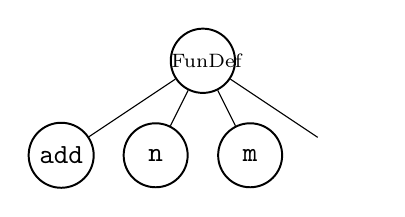
\begin{tikzpicture}[
    level distance=1.2cm,
    level 1/.style={sibling distance=1.2cm},
]
  \node [arn_u] {\scriptsize FunDef}
  child{
    node [arn_u] {\code{add}}
  }
  child{
    node [arn_u] {\code{n}}
  }
  child{
    node [arn_u] {\code{m}}
  }
  child{
    node [arn_w] {}
  };
\end{tikzpicture}
\end{center}

The root of the tree is the symbol FunDef, which explains that this tree
represents a function definition. The tree has four children: \code{add},
\code{n}, \code{m}, and the body expression. We do not know how to draw the tree
representing the body expression yet.

The body expression is an addition expression. It has two components: the
operands of the addition.

\begin{center}
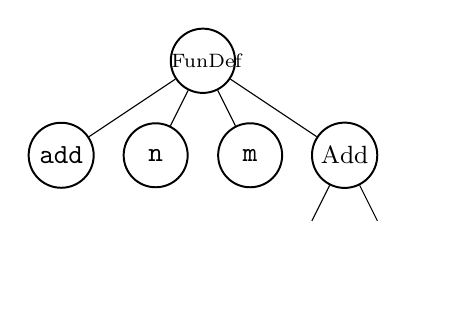
\begin{tikzpicture}[
    level distance=1.2cm,
    level 1/.style={sibling distance=1.2cm},
    level 2/.style={sibling distance=1.2cm}
]
  \node [arn_u] {\scriptsize FunDef}
  child{
    node [arn_u] {\code{add}}
  }
  child{
    node [arn_u] {\code{n}}
  }
  child{
    node [arn_u] {\code{m}}
  }
  child{
    node [arn_u] {\small Add}
    child{
      node [arn_w] {}
    }
    child{
      node [arn_w] {}
    }
  };
\end{tikzpicture}
\end{center}

The root of the tree is Add as the expression is addition. It has two
children: the operand expressions.

The first operand expression consists of a single component: \code{n}.

\begin{center}
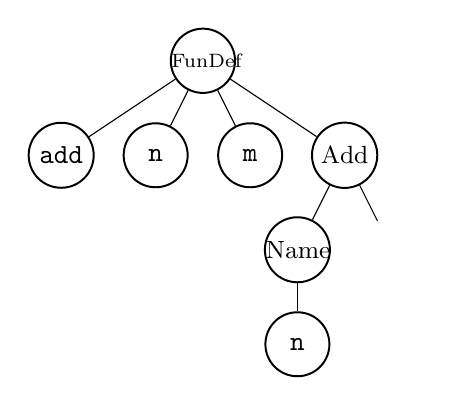
\begin{tikzpicture}[
    level distance=1.2cm,
    level 1/.style={sibling distance=1.2cm},
    level 2/.style={sibling distance=1.2cm}
]
  \node [arn_u] {\scriptsize FunDef}
  child{
    node [arn_u] {\code{add}}
  }
  child{
    node [arn_u] {\code{n}}
  }
  child{
    node [arn_u] {\code{m}}
  }
  child{
    node [arn_u] {\small Add}
    child{
      node [arn_u] {\small Name}
      child{
        node [arn_u] {\code{n}}
      }
    }
    child{
      node [arn_w] {}
    }
  };
\end{tikzpicture}
\end{center}

The root of the tree is Name, since the expression is just a name. The
only child is \code{n}.

The second operand expression can be similarly represented as a tree.

\begin{center}
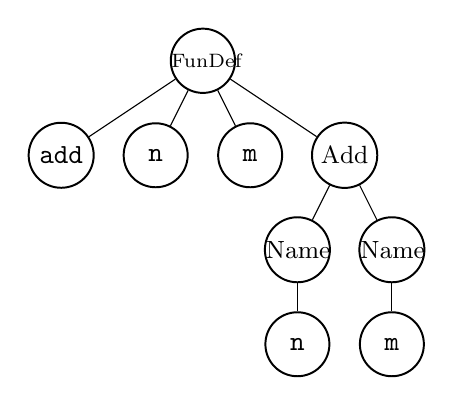
\begin{tikzpicture}[
    level distance=1.2cm,
    level 1/.style={sibling distance=1.2cm},
    level 2/.style={sibling distance=1.2cm}
]
  \node [arn_u] {\scriptsize FunDef}
  child{
    node [arn_u] {\code{add}}
  }
  child{
    node [arn_u] {\code{n}}
  }
  child{
    node [arn_u] {\code{m}}
  }
  child{
    node [arn_u] {\small Add}
    child{
      node [arn_u] {\small Name}
      child{
        node [arn_u] {\code{n}}
      }
    }
    child{
      node [arn_u] {\small Name}
      child{
        node [arn_u] {\code{m}}
      }
    }
  };
\end{tikzpicture}
\end{center}

The above tree represents the structure of the function definition. It is
independent of its underlying programming language. The tree can be a Python
function definition and a JavaScript function definition at the same time. By
expressing programs with trees, we can ignore unnecessary details in strings and
focus on the structures of programs.

As abstract syntax treats programs as trees, defining the abstract syntax of a
language is to define the set of every tree that represents a program. Let us
define the abstract syntax of \lang. In \lang, every natural number is a
program. A natural number program has only one component: the natural number
itself. Therefore, the following fact is true, where $E$ denotes the set of
every program:

\begin{center}
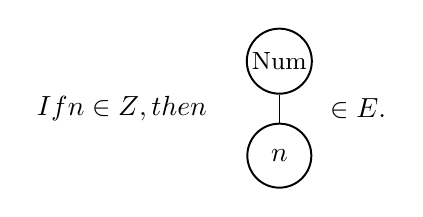
\begin{tikzpicture}[
    level distance=1.2cm,
    level 1/.style={sibling distance=1.2cm},
]
  \node at (-2,-0.6) {$\text{If }n\in\mathbb{Z}\text{, then}$};
  \node [arn_u] at (0,0) {\small Num}
  child{
    node [arn_u] {$n$}
  };
  \node at (1,-0.6) {$\in E$.};
\end{tikzpicture}
\end{center}

Addition of two arithmetic expressions is also a program. Such a program has
two components: the left and right operands. Each operand is an arithmetic
expression and thus a program. Therefore, the following fact is true:

\begin{center}
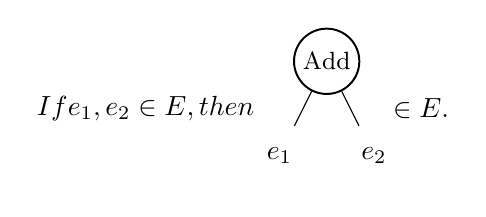
\begin{tikzpicture}[
    level distance=1.2cm,
    level 1/.style={sibling distance=1.2cm},
]
  \node at (-2.3,-0.6) {$\text{If }e_1,e_2\in E\text{, then}$};
  \node [arn_u] at (0,0) {\small Add}
  child{
    node [arn_nc] {$e_1$}
  }
  child{
    node [arn_nc] {$e_2$}
  };
  \node at (1.2,-0.6) {$\in E$.};
\end{tikzpicture}
\end{center}

Subtraction is similar.

\begin{center}
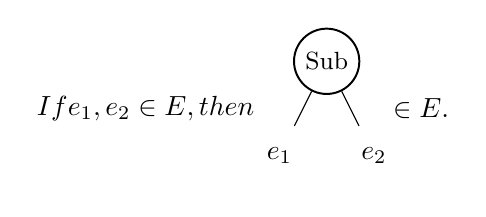
\begin{tikzpicture}[
    level distance=1.2cm,
    level 1/.style={sibling distance=1.2cm},
]
  \node at (-2.3,-0.6) {$\text{If }e_1,e_2\in E\text{, then}$};
  \node [arn_u] at (0,0) {\small Sub}
  child{
    node [arn_nc] {$e_1$}
  }
  child{
    node [arn_nc] {$e_2$}
  };
  \node at (1.2,-0.6) {$\in E$.};
\end{tikzpicture}
\end{center}

By collecting all the above facts, we can define the abstract syntax of \lang as
the smallest set $E$ satisfying the following conditions.

\begin{center}
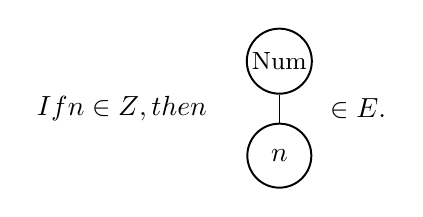
\begin{tikzpicture}[
    level distance=1.2cm,
    level 1/.style={sibling distance=1.2cm},
]
  \node at (-2,-0.6) {$\text{If }n\in\mathbb{Z}\text{, then}$};
  \node [arn_u] at (0,0) {\small Num}
  child{
    node [arn_u] {$n$}
  };
  \node at (1,-0.6) {$\in E$.};
\end{tikzpicture}
\end{center}

\begin{center}
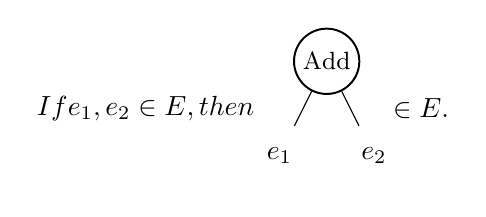
\begin{tikzpicture}[
    level distance=1.2cm,
    level 1/.style={sibling distance=1.2cm},
]
  \node at (-2.3,-0.6) {$\text{If }e_1,e_2\in E\text{, then}$};
  \node [arn_u] at (0,0) {\small Add}
  child{
    node [arn_nc] {$e_1$}
  }
  child{
    node [arn_nc] {$e_2$}
  };
  \node at (1.2,-0.6) {$\in E$.};
\end{tikzpicture}
\end{center}

\begin{center}
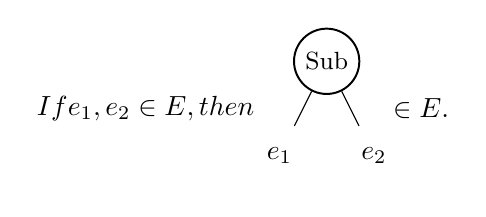
\begin{tikzpicture}[
    level distance=1.2cm,
    level 1/.style={sibling distance=1.2cm},
]
  \node at (-2.3,-0.6) {$\text{If }e_1,e_2\in E\text{, then}$};
  \node [arn_u] at (0,0) {\small Sub}
  child{
    node [arn_nc] {$e_1$}
  }
  child{
    node [arn_nc] {$e_2$}
  };
  \node at (1.2,-0.6) {$\in E$.};
\end{tikzpicture}
\end{center}

For example, the following tree represents an \lang program:

\begin{center}
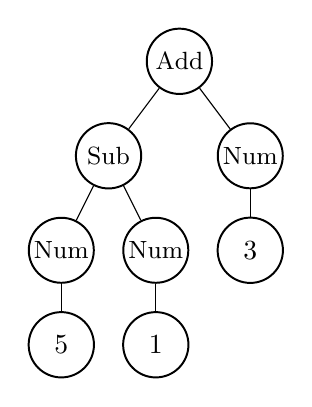
\begin{tikzpicture}[
    level distance=1.2cm,
    level 1/.style={sibling distance=1.8cm},
    level 2/.style={sibling distance=1.2cm},
]
  \node [arn_u] {\small Add}
  child{
    node [arn_u] {\small Sub}
    child{
      node [arn_u] {\small Num}
      child{
        node [arn_u] {$5$}
      }
    }
    child{
      node [arn_u] {\small Num}
      child{
        node [arn_u] {$1$}
      }
    }
  }
  child{
    node [arn_u] {\small Num}
    child{
      node [arn_u] {$3$}
    }
  };
\end{tikzpicture}
\end{center}

We call a tree that is an element of the set defined by abstract syntax an
\textit{abstract syntax tree}\index{abstract syntax tree} (\acrshort{astLabel}).

Abstract syntax can be easily implemented with ADTs in Scala. The following code
implements the abstract syntax of \lang:

\begin{verbatim}
sealed trait AE
case class Num(value: Int) extends AE
case class Add(left: AE, right: AE) extends AE
case class Sub(left: AE, right: AE) extends AE
\end{verbatim}

\code{Num($n$)} corresponds to

\begin{center}
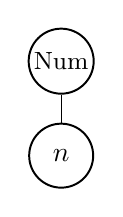
\begin{tikzpicture}[
    level distance=1.2cm,
    level 1/.style={sibling distance=1.2cm},
]
  \node [arn_u] {\small Num}
  child{
    node [arn_u] {$n$}
  };
\end{tikzpicture}
\end{center}

\code{Add($e_1$, $e_2$)} corresponds to

\begin{center}
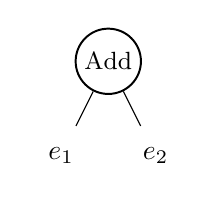
\begin{tikzpicture}[
    level distance=1.2cm,
    level 1/.style={sibling distance=1.2cm},
]
  \node [arn_u] {\small Add}
  child{
    node [arn_nc] {$e_1$}
  }
  child{
    node [arn_nc] {$e_2$}
  };
\end{tikzpicture}
\end{center}

\code{Sub($e_1$, $e_2$)} corresponds to

\begin{center}
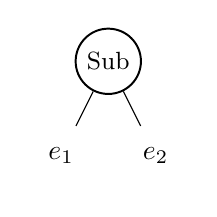
\begin{tikzpicture}[
    level distance=1.2cm,
    level 1/.style={sibling distance=1.2cm},
]
  \node [arn_u] {\small Sub}
  child{
    node [arn_nc] {$e_1$}
  }
  child{
    node [arn_nc] {$e_2$}
  };
\end{tikzpicture}
\end{center}

The previous AST can be written as \code{Add(Sub(Num(5),
Num(1)), Num(3))} in Scala.

It is inconvenient to draw a tree every time we need to express a program. For
this reason, people usually use notations that look like code to represent
trees. For example, we can simply write $n$ instead of drawing a tree whose root
is Num and only child is $n$ when it is clear that $n$ denotes an AST
from the context. Similarly, we can use $e_1+e_2$ and $e_1-e_2$
instead of trees that represent addition and subtraction, respectively. Note that
$+$ and $-$ in the notations are not the mathematical addition and subtraction
operators. They are just parts of the notations and do not have any meaning.

We can define the abstract syntax of \lang again by using the above notations.
$E$ is the smallest set satisfying the following conditions:

\begin{itemize}
  \item If $n\in\mathbb{Z}$, then $n\in E$.
  \item If $e_1,e_2\in E$, then $e_1+e_2\in E$.
  \item If $e_1,e_2\in E$, then $e_1-e_2\in E$.
\end{itemize}

Even though the notations themselves do not look like trees at all, they still
represent ASTs. Also, symbols like $+$ and $-$ do not have any meaning. It
is extremely important to keep these points in your mind. Otherwise, you will
mix abstract syntax using notations up with concrete syntax in the end.

Notations are just notations. You can define different notations and use them.
For example, one may use $\embox{ADD}\ e_1\ e_2$ instead of $e_1 + e_2$ to represent
addition. You can freely choose notations, but once you define them, you should
consistently use them not to make other people confused.

To make the definition of abstract syntax more concise, we adopt BNF to the
definition of abstract syntax. We can re-define the abstract syntax of \lang with
BNF:

\[e\ ::=\ n\ |\ e+e\ |\ e-e\]

We call each symbol that denotes a particular element in abstract syntax a
\textit{metavariable}.\index{metavariable}
It is called \textbf{meta}variable because it is a variable at a
meta-level, not the level of the defined programming language. For example, $e$
is a metavariable that ranges over programs, and $n$ is a metavariable that
ranges over integers.

We often use parentheses to express elements of abstract syntax without
ambiguity. For instance, $3-1+2$ can be interpreted in two ways:

\begin{center}
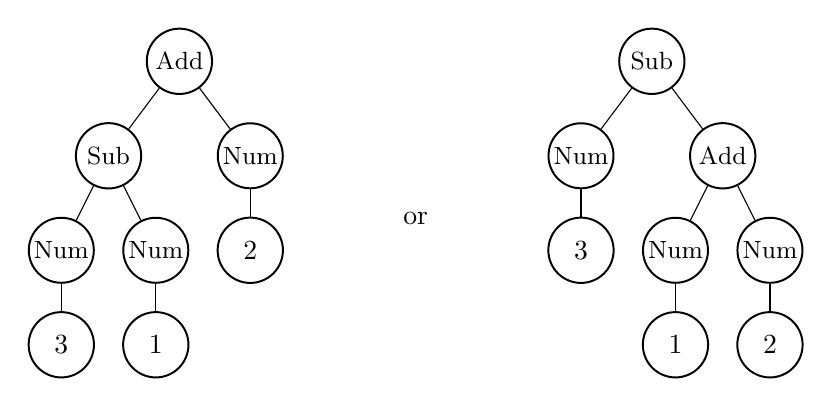
\begin{tikzpicture}[
    level distance=1.2cm,
    level 1/.style={sibling distance=1.8cm},
    level 2/.style={sibling distance=1.2cm},
]
  \node [arn_u] at (-3,0) {\small Add}
  child{
    node [arn_u] {\small Sub}
    child{
      node [arn_u] {\small Num}
      child{
        node [arn_u] {$3$}
      }
    }
    child{
      node [arn_u] {\small Num}
      child{
        node [arn_u] {$1$}
      }
    }
  }
  child{
    node [arn_u] {\small Num}
    child{
      node [arn_u] {$2$}
    }
  };
  \node at (0,-2) {or};
  \node [arn_u] at (3,0) {\small Sub}
  child{
    node [arn_u] {\small Num}
    child{
      node [arn_u] {$3$}
    }
  }
  child{
    node [arn_u] {\small Add}
    child{
      node [arn_u] {\small Num}
      child{
        node [arn_u] {$1$}
      }
    }
    child{
      node [arn_u] {\small Num}
      child{
        node [arn_u] {$2$}
      }
    }
  };
\end{tikzpicture}
\end{center}

If we write $(3-1)+2$, it is clear that it denotes the former. Otherwise, we
write $3-(1+2)$ to denote the latter.

\section{Parsing}

Concrete syntax considers programs as strings, while abstract syntax considers
programs as trees. Parsing bridges this gap. \textit{Parsing}\index{parsing} is
a process of transforming a string following concrete syntax into an AST. A
parser is a program that parses input. We can consider a parser as a partial
function from $S$ (the set of every string) to $E$ (the set of
every AST).

\[\embox{parse}: S\pto E\]

\begin{kaobox}[frametitle=Partial functions]
  A partial function from a set $A$ to a set $B$ is a function from a subset $S$ of
  $A$ to $B$. $S$ is called the domain of definition, or just domain in short, of the partial function.
  While $A\rightarrow B$ is a set of functions from $A$ to $B$, $A\pto B$ is a set
  of partial functions from $A$ to $B$.

  Let $f$ be a partial function from $A$ to $B$. Then, there can be $a\in A$ such
  that $f(a)$ is undefined. From a programmers' perspective, $f$ can be
  interpreted as a function from $A$ to \code{Option[$B$]}, where \code{None}
  means that the image is undefined and \code{Some($b$)} means that the image is
  $b$.
\end{kaobox}

The result of $\embox{parse}$
is undefined when an input does not belong to $P$ (the set of every
program). That is why $\embox{parse}$ is a partial function. When an input
belongs to $P$, $\embox{parse}$ results in its corresponding AST.

Consider the parser of \lang. The results of $\embox{parse}$ are undefined for
the following strings as they are not \lang programs:

\begin{itemize}
  \item \code{1+}
  \item \code{2*4}
  \item \code{0++3}
\end{itemize}

On the other hand, below is an example of when $\embox{parse}$ succeeds.

\begin{center}
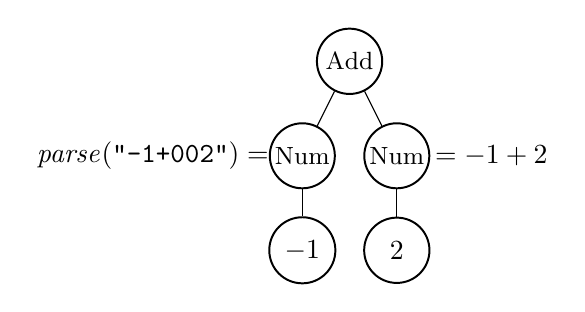
\begin{tikzpicture}[
    level distance=1.2cm,
    level 1/.style={sibling distance=1.2cm},
]
  \node at (-2.5,-1.2) {$\embox{parse}(\code{"-1+002"})=$};
  \node [arn_u] at (0,0) {\small Add}
  child{
    node [arn_u] {\small Num}
    child{
      node [arn_u] {$-1$}
    }
  }
  child{
    node [arn_u] {\small Num}
    child{
      node [arn_u] {$2$}
    }
  };
  \node at (1.8,-1.2) {$=-1+2$};
\end{tikzpicture}
\end{center}

This book does not discuss implementation of parsers.

\section{Semantics}

Syntax is an essential element of a programming language. It allows us to know
which strings are programs and what the structures of programs are. However,
syntax does not explain execution of programs. Programmers write programs to
execute them. They should know what will happen when their programs are
executed. Therefore, we need semantics in addition to syntax. Semantics is the
other essential element of a programming language. It defines the behaviors of
programs.

Let us define the semantics of \lang. Semantics is defined based on abstract
syntax. The structure of a program determines its behavior. Since abstract
syntax represents the structure, it is natural to use abstract syntax for
semantics. The semantics of \lang defines the semantics of each \lang program,
where the semantics of a program means things that happen when the program is
executed. When an \lang program is executed, it does one thing: outputs the
result of the evaluation of the arithmetic expression.
For example, $0+1$ should result
in $1$ if the semantics is defined correctly. Note that $+$ in $0+1$ does not
mean addition, and we cannot say anything about the result of $0+1$ until the
semantics is defined. To make \lang a reasonable language, we must define the
semantics of \lang so that $0+1$ results in $1$.

There are infinitely many programs. We cannot define the semantics of each
program separately. We need to utilize the structures of programs defined by the
abstract syntax. According to the abstract syntax, programs can split into three
groups: $n$, $e_1+e_2$, and $e_1-e_2$. By defining the semantics of each group
once, we can complete the semantics of infinitely many programs in a finite
method.

The simplest case is $n$. $n$ is an expression consisting of an integer. An
integer evaluates to itself. We represent this semantics as the following rule:

\semanticrule{Num}{
$n$ evaulates to $n$.
}

We can conclude the following facts by using Rule \textsc{Num}.

\begin{itemize}
  \item $1$ evaulates to $1$.
  \item $5$ evaulates to $5$.
\end{itemize}

The next case is $e_1+e_2$. As $e_1$ is an arithmetic expression, it results in
some integer. Let $n_1$ be the integer. Similarly, $e_2$ also results in some
integer. Let $n_2$ be the integer. Then, the result of $e_1+e_2$ is the sum of
$n_1$ and $n_2$. In this chapter, we use $\iadd$ instead of $+$ to denote
mathematical addition. It will help you distinguish mathematical addition from
$+$ used for the abstract syntax. Once you become familiar with syntax and
semantics, you can easily distinguish them by checking the context even if both
are denoted by $+$. From the next chapter, we will use $+$ for both abstract
syntax and mathematical addition. The following rule defines the semantics of
$e_1+e_2$.

\semanticrule{Add}{
If $e_1$ evaluates to $n_1$, and $e_2$ evaluates to $n_2$,\\
then $e_1+e_2$ evaluates to $n_1\iadd n_2$.
}

We can define the semantics of $e_1-e_2$ in a similar way. Like $\iadd$,
we use $\isub$ for mathematical subtraction in this chapter. The
following rule defines the semantics of $e_1-e_2$.

\semanticrule{Sub}{
If $e_1$ evaluates to $n_1$, and $e_2$ evaluates to $n_2$,\\
then $e_1-e_2$ evaluates to $n_1\isub n_2$.
}

These three rules are all of the semantics of \lang. We now know the behavior of
every \lang program. For example, consider $(3-1)+2$. The following steps
show why $(3-1)+2$ evaluates to $4$.

\begin{enumerate}
  \item (By Rule \textsc{Num}) $3$ evaluates to $3$.
  \item (By Rule \textsc{Num}) $1$ evaluates to $1$.
  \item (By Rule \textsc{Sub}) If $3$ evaluates to $3$ and $1$ evaluates to $1$, then $3-1$
    evaluates to $2$.
  \item (By 1, 2, and 3) $3-1$ evaluates to $2$.
  \item (By Rule \textsc{Num}) $2$ evaluates to $2$.
  \item (By Rule \textsc{Add}) If $3-1$ evaluates to $2$ and $2$ evaluates to $2$, then
    $(3-1)+2$ evaluates to $4$.
  \item (By 4, 5, and 6) $(3-1)+2$ evaluates to $4$.
\end{enumerate}

Now, let us define the semantics of \lang in a more mathematical way. The
semantics defines the result of the execution of each program. Here, the result
is an integer. We can say that semantics outputs an integer when a program is
given. Thus, the semantics can be considered as a function from a program to an
integer.

\[\embox{eval}:E\rightarrow \mathbb{Z}\]

For each $e\in E$, there should exist a unique integer $\embox{eval}(e)$. It
is obviously true in \lang. Every arithmetic expression evaluates to a unique
integer.

However, defining semantics as a function is a bad choice in other languages.
Some programs do not produce any results. Nonterminating programs are such
examples. Programs that incur run-time errors also belong to this category. You
will see programs with run-time errors in the next chapter. Moreover, there is a
program whose result is not unique. We call such programs nondeterministic
programs. For example, the behavior of a concurrent program with multiple
threads depends on how the threads are interleaved during execution. If the
threads are interleaved differently, the result may change. Programs without
results and nondeterministic programs prevent us from defining semantics as a
function. We should define semantics as a relation. Even though the semantics of
\lang can be defined as a function, we define the semantics as a relation to
make the discussion of this chapter easily extendable to other languages.

We define the semantics of \lang as $\Rightarrow$, a binary relation over $E$
and $\mathbb{Z}$.

\begin{kaobox}[frametitle=Binary relations]
A binary relation over sets $A$ and $B$ is a subset of $A\times B$,
where $A\times B=\{(a,b)\ |\ a\in A\land b\in B\}$.

Let $R$ be a binary relation over $A$ and $B$. Then, $R \subseteq A\times B$. For $a\in
A$ and $b\in B$, we write $a\ R\ b$ when $(a,b)\in R$. For example, $<$ is a
binary relation over $\mathbb{Z}$ and $\mathbb{Z}$, and we can write $1<2$ instead of
$(1,2)\in<$.
\end{kaobox}

\[\Rightarrow\subseteq E\times\mathbb{Z}\]

$(e,n)\in\Rightarrow$, i.e. $e\Rightarrow n$ implies that $e$ evaluates to $n$.

Let us define the semantics again with mathematical concepts.

\semanticrule{Num}{
$n\Rightarrow n$.
}

\vspace{-1em}

\semanticrule{Add}{
If $e_1\Rightarrow n_1$ and $e_2\Rightarrow n_2$,\\
then $e_1+e_2\Rightarrow n_1\iadd n_2$.
}

\vspace{-1em}

\semanticrule{Sub}{
If $e_1\Rightarrow n_1$ and $e_2\Rightarrow n_2$,\\
then $e_1-e_2\Rightarrow n_1\isub n_2$.
}

We use one more mathematical concept: inference rules. An \textit{inference
rule}\index{inference rule} is a rule to prove a new proposition from given
propositions. An inference rule has the following form:

\[
  \inferrule
  { \embox{premise}_1 \\ \embox{premise}_2 \\ \cdots \\ \embox{premise}_n }
  { \embox{conclusion} }
\]

It consists of a horizontal line, propositions above the line, and a proposition
below the line. We call the propositions above the line
\textit{premises}\index{premise} and the proposition below the line a
\textit{conclusion}\index{conclusion}. The rule means that if every premise is
true, then also the conclusion is true. A single inference rule can have zero or
more premises. A rule without premises implies that its conclusion is always
true. When a rule does not have any premises, we can omit the horizontal line.

Let us define the semantics of \lang with inference rules.

\[
  n\Rightarrow n
  \quad\textsc{[Num]}
\]

\[
  \inferrule
  { e_1\Rightarrow n_1 \\ e_2\Rightarrow n_2 }
  { e_1+e_2\Rightarrow n_1\iadd n_2 }
  \quad\textsc{[Add]}
\]

\[
  \inferrule
  { e_1\Rightarrow n_1 \\ e_2\Rightarrow n_2 }
  { e_1-e_2\Rightarrow n_1\isub n_2 }
  \quad\textsc{[Sub]}
\]

As you can see, the rules are much clearer and more concise than the rules
written in a natural language.

We can prove $(3-1)+2\Rightarrow4$ with the rules. We usually draw a proof tree
when we prove a proposition with inference rules. A \textit{proof
tree}\index{proof tree} is a tree whose root is the proposition to be proven.
Each node of the tree is a proposition, and the children nodes of a node are
evidences supporting that the proposition of the node is true. Unlike most trees in
computer science, we place the root of a proof tree at the bottom. Every node is
placed below its children.

The following proof tree proves $3\Rightarrow3$.

\[3\Rightarrow3\]

The tree has only the root node because Rule \textsc{Num} does not have any
premises.

Similarly, the following proof tree proves $1\Rightarrow1$.

\[1\Rightarrow1\]

We draw the following proof tree with Rule \textsc{Sub} and the above trees
to prove $3-1\Rightarrow2$.

\[
  \inferrule
  { 3\Rightarrow3 \\ 1\Rightarrow1 }
  { 3-1\Rightarrow2 }
\]

By using Rule \textsc{Num} again, we prove $2\Rightarrow2$.

\[2\Rightarrow2\]

Finally, we get the proof tree of $(3-1)+2\Rightarrow4$.

\[
  \inferrule
  {
    \inferrule
    { 3\Rightarrow3 \\ 1\Rightarrow1 }
    { 3-1\Rightarrow2 }
    \\
    2\Rightarrow2
  }
  { (3-1)+2\Rightarrow4 }
\]

To explain what proof trees are, we have drawn the proof tree from its leaf
nodes. However, we usually draw a proof tree from the root node.
We start by drawing a horizontal line and writing the program we want to evaluate.

\[
  \inferrule
  {
    \color{white}
    \inferrule
    { 3\Rightarrow3 \\ 1\Rightarrow1 }
    { 3-1\Rightarrow2 }
    \\
    \color{white}
    2\Rightarrow2
  }
  { (3-1)+2\Rightarrow{\color{white}4} }
\]

Then, we find which inference rule can be applied. In this case, we can use Rule
\textsc{Add} since the program is addition.

\[
  \inferrule
  {
    \inferrule
    { \color{white}3\Rightarrow3 \\ \color{white}1\Rightarrow1 }
    { 3-1\Rightarrow\color{white}2 }
    \\
    2\Rightarrow\color{white}2
  }
  { (3-1)+2\Rightarrow{\color{white}4} }
\]

We need to evaluate $3-1$ and $2$ respectively. Let us focus on $3-1$ first.
Since $3-1$ is subtraction, we use Rule \textsc{Sub}.

\[
  \inferrule
  {
    \inferrule
    { 3\Rightarrow\color{white}3 \\ 1\Rightarrow\color{white}1 }
    { 3-1\Rightarrow\color{white}2 }
    \\
    2\Rightarrow\color{white}2
  }
  { (3-1)+2\Rightarrow{\color{white}4} }
\]

We can conclude that $3\Rightarrow3$ from Rule \textsc{Num}.

\[
  \inferrule
  {
    \inferrule
    { 3\Rightarrow3 \\ 1\Rightarrow\color{white}1 }
    { 3-1\Rightarrow\color{white}2 }
    \\
    2\Rightarrow\color{white}2
  }
  { (3-1)+2\Rightarrow{\color{white}4} }
\]

Similarly, $1\Rightarrow1$.

\[
  \inferrule
  {
    \inferrule
    { 3\Rightarrow3 \\ 1\Rightarrow1 }
    { 3-1\Rightarrow\color{white}2 }
    \\
    2\Rightarrow\color{white}2
  }
  { (3-1)+2\Rightarrow{\color{white}4} }
\]

By subtracting $1$ from $3$, we get $2$.

\[
  \inferrule
  {
    \inferrule
    { 3\Rightarrow3 \\ 1\Rightarrow1 }
    { 3-1\Rightarrow2 }
    \\
    2\Rightarrow\color{white}2
  }
  { (3-1)+2\Rightarrow{\color{white}4} }
\]

We use Rule \textsc{Num} agian and get $2\Rightarrow2$.

\[
  \inferrule
  {
    \inferrule
    { 3\Rightarrow3 \\ 1\Rightarrow1 }
    { 3-1\Rightarrow2 }
    \\
    2\Rightarrow2
  }
  { (3-1)+2\Rightarrow{\color{white}4} }
\]

Finally, we can complete the proof tree and prove $(3-1)+2\Rightarrow4$.

\[
  \inferrule
  {
    \inferrule
    { 3\Rightarrow3 \\ 1\Rightarrow1 }
    { 3-1\Rightarrow2 }
    \\
    2\Rightarrow2
  }
  { (3-1)+2\Rightarrow4 }
\]

Sometimes, we call a proof tree proving the result of a program a
\textit{evaluation derivation}\index{evaluation derivation}
since the tree explains how the result of the program is derived.

The way of defining semantics we have seen so far is \textit{big-step
operational semantics}.\index{big-step operational semantics} It is called
``operational'' because it focuses on which \textbf{operation}s happen during execution
and ``big-step'' because it finds the result of a program by taking a single
\textbf{big} step. There are other ways to define semantics: denotational
semantics and small-step operational semantics. Most part of this book uses
big-step operational semantics. However, it will use small-step operational
semantics to deal with continuations later.

An \textit{interpreter}\index{interpreter} is a program that takes a program as
input and evaluates the program. We can easily implement an interpreter of
\lang according to its semantics. The interpreter consists of a single function
that takes an AST as an argument and returns an integer.

\begin{verbatim}
def interp(e: AE): Int = e match {
  case Num(n) => n
  case Add(l, r) => interp(l) + interp(r)
  case Sub(l, r) => interp(l) - interp(r)
}
\end{verbatim}

\section{Syntactic Sugar}

\textit{Syntactic sugar}\index{syntactic sugar} adds a new feature to a language
by defining syntactic transformation rules instead of changing the semantics.
Syntactic sugar is widely used in real-world programming languages because it
allows languages to provide useful features without increasing the burden of the
language designers too much.

Suppose that we want to add integer negation to \lang. It can be done by
modifying both syntax and semantics of \lang. First, we fix the concrete syntax
to add integer negation.

\begin{verbatim}
<expr> ::= <number> | <expr> "+" <expr>
         | <expr> "-" <expr> | "-" "(" <expr> ")"
\end{verbatim}

Similarly, we fix the abstract syntax, too.

\[e\ ::=\ n\ |\ e+e\ |\ e-e\ |\ -e\]

The parser should be changed accordingly. For example, \code{-(03+4)} is parsed
to $-(3+4)$.

Finally, we add a new rule to the semantics to handle the $-e$ case.

\semanticrule{Neg}{
If $e$ evaluates to $n$,\\
then $-e$ evaluates to $\isub n$.
}

Note that $\isub$ denotes mathematical negation.

We can express the same thing as an inference rule.

\[
  \inferrule
  { e\Rightarrow n}
  { -e\Rightarrow\isub n }
  \quad\textsc{Neg}
\]

It requires considerable amount of work as we need to fix every component of the language.

Another way to add integer negation to \lang is to add it as syntactic sugar. It
is enough to modify the concrete syntax and the parser. The change in the
concrete syntax is the same as before. Now, we fix the parser to parse \code{"-"
"(" expr ")"} to $0-e$ when \code{expr} is parsed to $e$. For example,
\code{-(03+4)} is parsed to $0-(3+4)$. Since $0\isub n=\isub n$ for any integer
$n$, we are done. It is the power of syntactic sugar. Language designers can
easily add new features by syntactically transforming them to existing features.
The procedure removing syntactic sugar by transformation is called
\textit{desugaring}\index{desugaring}.

We can find various examples of syntactic sugar in real-world languages. For
instance, for loops in Scala are supported as syntactic sugar.

\begin{quote}
  A for comprehension \code{for ($p$ <- $e$) yield $e'$} is translated to
  \code{$e$.map \{ case $p$ =>
  $e'$ \}}.\sidenote{\url{https://www.scala-lang.org/files/archive/spec/2.13/06-expressions.html\#for-comprehensions-and-for-loops}}
\end{quote}

In addition, macros in languages like C, Scala, LISP, and Rust can be considered
as user-defined syntactic sugar.

\section{Exercises}

\begin{exercise}
\labex{syntax-and-semantics-expr}

Consider the following concrete syntax:

\begin{verbatim}
<expr> ::= <num>
         | "{" "+" <expr> <expr> "}"
         | "{" "*" <expr> <expr> "}"
         | "{" "let" "{" <id> <expr> "}" <expr> "}"
         | <id>
\end{verbatim}

Describe whether each of the following is \code{expr} and why.
\code{<id>} consists of one or more latin alphabets (\code{a-z}, \code{A-Z}), and
\code{<num>} consists of one or more digits (\code{0-9}).
Assume that it is allowed to add whitespaces among terminals freely.

\begin{enumerate}
  \item \verb!{let {x 5} {+ 8 {* x 2 3}}}!
  \item \verb!{with {x 0} {with {x 7}}}!
  \item \verb!{let {3 5} {+ 8 {- x 2}}}!
  \item \verb!{let {3 y} {+ 8 {* x 2}}}!
  \item \verb!{let {x y} {+ 8 {* x 2}}}!
\end{enumerate}

\end{exercise}

\begin{exercise}
\labex{syntax-and-semantics-icecream}

Consider the following concrete syntax:

\begin{verbatim}
<ice-cream> ::= "sprinkles" "on" <ice-cream>
              | "cherry" "on" <ice-cream>
              | "scoop" "of" <flavor> "on" <ice-cream>
              | "sugar-cone"
              | "waffle-cone"
<flavor>    ::= "vanilla"
              | "lettuce"
\end{verbatim}

Assume that it is allowed to add whitespaces among terminals freely.
Describe whether each of the following is \code{<ice-cream>} and why.

\begin{enumerate}
  \item \code{sprinkles}
  \item \code{sugar-cone}
  \item \code{vanilla}
  \item \code{scoop of vanilla on waffle-cone}
  \item \code{sprinkles on lettuce on waffle-cone}
  \item \code{scoop of vanilla on sprinkles on waffle-cone}
  \item \code{cherry on scoop of lettuce on scoop of vanilla on sugar-cone}
\end{enumerate}

\end{exercise}

\begin{exercise}
\labex{syntax-and-semantics-coffee}

Consider the following concrete syntax:

\newcommand{\BNF}[1]{\code{<#1>}}
\newcommand{\coffee}{\mbox{\BNF{coffee}}}
\newcommand{\milk}{\mbox{\BNF{milk}}}
\newcommand{\flavor}{\mbox{\BNF{flavor}}}

\[
\begin{array}{ccc}
  \code{espresso} \in \coffee
  &&
  \inferrule
  { e_1 \in \milk \\ e_2 \in \coffee }
  { e_1\ \code{"on"}\ e_2 \in \coffee }
  \\[2em]
  \inferrule
  { e_1 \in \coffee \\ e_2 \in \milk }
  { e_1\ \code{"on"}\ e_2 \in \coffee }
  &&
  \inferrule
  { e_1 \in \flavor \\ e_2 \in \coffee }
  { e_1\ \code{"on"}\ e_2 \in \coffee }
  \\[2em]
  \code{"milk-foam"} \in \milk
  &&
  \code{"steamed-milk"} \in \milk
  \\[2em]
  \code{"caramel"} \in \flavor
  &&
  \code{"cinnamon"} \in \flavor
  \\[2em]
  \code{"cocoa-powder"} \in \flavor
  &&
  \code{"chocolate-syrup"} \in \flavor
\end{array}
\]

Assume that it is allowed to add whitespaces among terminals freely.
Describe whether each of the following is \code{<coffee>} and why.

\begin{enumerate}
  \item \code{caramel latte macchiato}
  \item \code{espresso}
  \item \code{steamed-milk on caramel on milk-foam on espresso}
  \item \code{chocolate-syrup on cocoa-powder on cinnamon on milk-foam on steamed-milk on espresso}
  \item \code{steamed-milk on espresso on chocolate-syrup}
  \item \code{cocoa-powder on milk-foam on steamed-milk on espresso}
\end{enumerate}

\end{exercise}

\begin{exercise}
\labex{syntax-and-semantics-pair}

This exercise extends \lang with pairs. Consider the following language:
\[
\begin{array}{rrl}
  e & ::= & \cdots\ |\ (e,e)\ |\ e\textsf{.1}\ |\ e\textsf{.2} \\
  v & ::= & \cdots\ |\ (v,v)
\end{array}
\]
The semantics is as follows:
\begin{itemize}
  \item The evaluation of $(e_1,e_2)$
    yields $(v_1,v_2)$, where $e_i$ evaluates to $v_i$.
  \item The evaluation of $e\textsf{.1}$ yields the first value of
    a pair $v$, where $e$ evalutes to $v$.
  \item The evaluation of $e\textsf{.2}$ yields the second value of
    a pair $v$, where $e$ evalutes to $v$.
\end{itemize}

\begin{enumerate}
  \item Write the operational semantics of the form \fbox{$e\Rightarrow v$}.
  \item Write the evaluation derivation of $(8,(320,42)\textsf{.1})\textsf{.2}$.
\end{enumerate}

\end{exercise}

\begin{exercise}
\labex{syntax-and-semantics-record}

This exercise extends \lang with records. A record is a value that maps labels to values.
Consider the following language:
\[
\begin{array}{rrl}
  e & ::= & \cdots\ |\ \{l:e,\cdots,l:e\}\ |\ e.l\\
  v & ::= & \cdots\ |\ \langle l:v,\cdots,l:v\rangle \\
\end{array}
\]
where $l$ ranges over labels.

The semantics is as follows:
\begin{itemize}
  \item The evaluation of $\{l_1:e_1,\cdots,l_n:e_n\}$
    yields $\langle l_1:v_1,\cdots,l_n:v_n\rangle$,
    where $e_i$ evaluates to $v_i$.
  \item The evaluation of $e.l$ yields the value of a field $l$
    in a record $v$, where $e$ evaluates to $v$.
\end{itemize}

Write the operational semantics of the form \fbox{$e\Rightarrow v$}.

\end{exercise}

\begin{exercise}
\labex{syntax-and-semantics-stlist}

This exercise extends \lang with JavaScript-like
sequencing.\sidenote{\url{https://tc39.es/ecma262/\#sec-block-runtime-semantics-evaluation}}
Consider the following language:
\[
  \begin{array}{rrl}
    e & ::= & \cdots\ |\ \textsf{()}\ |\ e;\cdots;e \\
    v & ::= & \cdots\ |\ \textsf{()} \\
  \end{array}
\]
The semantics is as follows:
\begin{itemize}
  \item
The value of $\textsf{()}$ is $\textsf{()}$.
  \item
The value of $e_1;\cdots;e_n$ is $\textsf{()}$
if every $e_i$ evaluates to $\textsf{()}$.
  \item
The value of $e_1;\cdots;e_n$
is the value of the last expression whose value is not $\textsf{()}$
if there is such an expression.
\end{itemize}
Write the operational semantics of the form \fbox{${e}\Rightarrow{v}$}.

\end{exercise}


\chapter{Identifiers}
\labch{identifiers}

\renewcommand{\plang}{\textsf{AE}\xspace}
\renewcommand{\Lang}{\textsf{VAE}\xspace}

Variables are one of the basic concepts of programming languages. A
\textit{variable}\index{variable} relates a name to a value. We use the
value of a variable by writing the name of the variable. For example, the following Scala program
prints \code{3}.

\begin{verbatim}
val x = 3
println(x)
\end{verbatim}

The program defines a variable whose name is \code{x} and value is \code{3}. At
the second line, the name \code{x} denotes the value \code{3}.

We call the names of variables identifiers. An
\textit{identifier}\index{identifier} is a name related to a
certain entity in a program. Not only the names of variables are identifiers;
there are various kinds of identifiers:

\begin{itemize}
\item Function names, which are related to functions
\item Parameter names, which are related to the values of arguments
\item Field names, which are related to values of fields
\item Method names, which are related to methods
\item Class names, which are related to classes
\end{itemize}

This chapter introduces identifiers. Identifiers in programs can split into
three groups: binding occurrences, bound occurrences, and free identifiers.
We will see what they are. This chapter discusses identifiers based on the use
of variables in programs. We will define \Lang by extending \plang of
\refch{syntax-and-semantics} with variables. Variables of \Lang are immutable.
We will deal with mutable variables in \refch{mutable-variables}.
In \Lang, the names of variables are
the only identifiers. However, as you have seen already, real-world programming
languages have many kinds of identifiers.

\section{Identifiers}

Identifiers name entities like variables and functions.
Let us discuss notions related to identifiers with the following Scala program:

\begin{verbatim}
f(0)
def f(x: Int): Int = {
  val y = 2
  x + y
}
f(1)
x - z
\end{verbatim}

In this program, \code{f}, \code{x}, \code{y}, and \code{z} are identifiers. Strictly speaking,
\code{Int} also is an identifier, but we ignore it because we do not want to take
types into account here.

A single identifier can occur multiple times in a program. For instance,
\code{f} occurs three times in the program: line 1, line 2, and line 6.
We can classify occurrences of identifiers into three categories:
binding occurrences, bound occurrences, and free identifiers.

An occurrence of an identifier is called a \textit{binding occurrence}\index{binding occurrence}
if the identifier occurs to be defined. A binding occurrence relates the
identifier to a particular entity. The program has three binding occurrences:

\begin{itemize}
  \item \code{f} at line 2

    It relates \code{f} to a function.

  \item \code{x} at line 2

    It relates \code{x} to the value of an argument given to \code{f}.

  \item \code{y} at line 3

    It relates \code{y} to the value \code{2}.
\end{itemize}

Every binding occurrence has its own scope. The \textit{scope}\index{scope} of a binding
occurrence means a code region where the identifier defined by the binding
occurrence is alive, i.e. usable. The scope of each identifier in the program is as follows:

\begin{itemize}
  \item \code{f}

    A function can be used in its body (as Scala allows recursive function
    definitions) and at the lines below its definition. The scope of
    \code{f} is from line 3 to line 7.

  \item \code{x}

    A parameter of a function can be used only in the function body. The scope of
    \code{x} is line 3 and line 4.

  \item \code{y}

    A variable can be used at the lines below its definition. The scope of
    \code{y} is line 4.
\end{itemize}

An occurrence of an identifier is called a \textit{bound occurrence}\index{bound occurrence}
if the identifier occurs to use the entity related to itself. Since an
identifier becomes related to an entity by its binding occurrence, any bound
occurrences must reside in the scope of the binding occurrence.
The program has three bound occurrences:

\begin{itemize}
  \item \code{f} at line 6

    It denotes the function defined at line 2.

  \item \code{x} at line 4

    It denotes the value of an argument passed to \code{f}.

  \item \code{y} at line 4

    It denotes the value \code{2}.
\end{itemize}

An occurrence of an identifier is called a \textit{free identifier}\index{free
identifier} if it is
neither binding nor bound. A free identifier neither introduces a new name nor
uses a name defined already. It is not in the scope of any binding occurrence of
the same identifier. The program has three free identifiers:

\begin{itemize}
  \item \code{f} at line 1

    It is outside the scope of \code{f}.

  \item \code{x} at line 7

    It is outside the scope of \code{x}.

  \item \code{z} at line 7

    The program never defines \code{z}.
\end{itemize}

We call a free identifier a \textit{free variable}\index{free variable} when it
is the name of a variable. Therefore, both \code{x} and \code{z} at line 7 are
free variables.

Now, consider a binding occurrence that resides in the scope of a binding
occurrence of the same identifier. For example, the following program has two
binding occurrences of \code{x}, and the second binding occurrence is in the
scope of the first binding occurrence.

\begin{verbatim}
def f(x: Int): Int = {
  def g(x: Int): Int =
    x
  g(x)
}
\end{verbatim}

In this case, shadowing happens. \textit{Shadowing}\index{shadowing} means that
the innermost binding occurrence \textbf{shadow}s, i.e. temporarily invalidates,
the outer binding occurrences of the same name. Therefore, \code{x} at line 2
shadows \code{x} at line 1.
\code{x} at line 3 belongs to the scope of both binding occurrences simultaneously.
It denotes the value of an argument given to \code{g}, not \code{f}, because of
shadowing. On the other hand, \code{x} at line 4 denotes the value of an
argument given to \code{f} since it belongs to the scope of only \code{x} at
line 1.

\section{Syntax}

Let us define the abstract syntax of \Lang. We do not consider concrete
syntax anymore. Therefore, the term syntax will be used to mean abstract
syntax. Also, from now on, we use the term
\textit{expressions}\index{expression} rather than
programs when we discuss languages like \Lang. For example, we say that
$1+2$ is an expression of \plang, and $1$ and $2$ are the subexpressions of
$1+2$.

Recall the example at the beginning of the chapter:

\begin{verbatim}
val x = 3
println(x)
\end{verbatim}

To add variables to \plang, we need two kinds of expressions. The first kind is
expressions defining a variable, i.e. binding an identifier. In the example,
\code{val x = 3; println(x)} is such an expression. It defines the
variable \code{x} and starts the scope of \code{x} so that \code{x} can be used
in \code{println(x)}. We can conclude that an expression defining a variable
consists of three parts: the name of the variable, an expression determining the
value of the variable, and an expression that can use the variable. These parts
are \code{x}, \code{3}, and \code{println(x)}, respectively, in the example. The
second kind is expressions using a variable, i.e. a bound occurrence. In the
example, \code{x} at the second line is such an expression. It uses the variable \code{x} to denote
the value \code{3}. Based on this observation, we can define the syntax of
\Lang.

First, we need to add a new syntactic element: identifiers. The metavariable
$x$ ranges over identifiers. Let $\embox{Id}$ be the set of every
identifier.

\[x\in\embox{Id}\]

We do not care what $\embox{Id}$ really is.

The syntax of \Lang is as follows:\footnote{We omit the common part
to \plang.}

\[e\ ::=\ \cdots\ |\ \ebind{x}{e}{e}\ |\ x\]

\begin{itemize}
  \item $\ebind{x}{e_1}{e_2}$

    It defines a new variable whose name is $x$. Therefore, the occurrence of $x$ is a
    binding occurrence. $e_1$ decides the value denoted by the variable. The
    scope of the variable includes $e_2$ but excludes $e_1$.

  \item $x$

    It uses a variable; it is either a bound occurrence of $x$ or a free identifier.
    If it belongs to the scope of a binding occurrence of the same name, then it is a
    bound occurrence and denotes the value associated with the identifier.
    Otherwise, it is a free identifier, which denotes nothing.
\end{itemize}

\section{Semantics}

To define the semantics of \Lang, we need an additional semantic element that
stores the values denoted by variables. Without such an element, we cannot know the
value of each variable. We call the element an
\textit{environment}\index{environment}. An environment is a finite partial
function.\footnote{A finite partial function is a partial function whose domain
is a finite set.} The metavariable $\sigma$ ranges over environments.

\[\embox{Env}=\embox{Id}\finto\mathbb{Z}\]
\[\sigma\in\embox{Env}\]

For example, consider an environment $\sigma$.
If $\sigma(\cx)=1$, the value of a variable named \code{x} is $1$.
An environment is a partial function because it does not have the values
related to free identifiers. If a variable named \code{y} is free in
$\sigma$, then $\sigma(\cy)$ is undefined.
In addition, it is finite since every program
defines only finitely many identifiers.

Every expression in \Lang can evaluate to an integer only under some
environment. The reason is obvious: without environments, there is no way to
find the values of variables, and thus environments are essential to evaluation.

The following rule defines the semantics of $x$:

\semanticrule{Id}{
If
  $x$ is in the domain of $\sigma$,\\
then
  \evaldn{x}{\sigma(x)}.
}

If $x$ is an element of the domain of $\sigma$, $x$ is a bound occurrence. The
environment gives us the value denoted by $x$, which is $\sigma(x)$. Then, the
result is $\sigma(x)$. Otherwise, $x$ is not in the domain and is a free
identifier. In that case, we cannot evaluate $x$. The evaluation terminates
immediately. It can be interpreted as a run-time error.

Formally, the semantics of \Lang is a
ternary relation over $\embox{Env}$, $E$, and $\mathbb{Z}$ since it must take
environments into account.

\[\Rightarrow\subseteq\embox{Env}\times E\times\mathbb{Z}\]

$(\sigma,e,n)\in\Rightarrow$ is true if and only if
$e$ evaluates to $n$ under $\sigma$.
We write $\sigma\vdash e\Rightarrow n$ instead of $(\sigma,e,n)\in\Rightarrow$.
Intuitively, $\sigma$ and $e$ are inputs, and $n$ is the corresponding output.

Rule \textsc{Id} can be formulated as the following inference rule:
\footnote{$\dom{\sigma}$ denotes the domain of $\sigma$.}

\[
  \inferrule
  { x\in\dom{\sigma} }
  { \evald{x}{\sigma(x)} }
  \quad\textsc{[Id]}
\]

When a variable is defined, the value of the variable is added to the environment.
We write $\sigma[x\mapsto n]$ to denote an environment obtained by adding the
fact that $x$ denotes $n$ to $\sigma$. Then, the following property holds:

\[
\sigma [x\mapsto n](x') =
\begin{cases}
  n & \text{if}\ x=x' \\
  \sigma(x') & \text{if}\ x\neq x'
\end{cases}
\]

The following rule defines the semantics of $\ebind{x}{e_1}{e_2}$:

\semanticrule{Val}{
If
  \evaldn{e_1}{n_1}, and
  \evaln{\sigma[x\mapsto n_1]}{e_2}{n_2},\\
then
  \evaldn{\ebind{x}{e_1}{e_2}}{n_2}.
}

To evaluate $\ebind{x}{e_1}{e_2}$, we need to determine the value of $x$ first.
It can be done by evaluating $e_1$. Since the scope of $x$ excludes $e_1$,
the evaluation proceeds under $\sigma$, which is a given environment.
The result of $e_1$ is the value of $x$, and this information must be added to
the environment. By adding the fact to $\sigma$, we get $\sigma[x\mapsto n_1]$.
As $e_2$ is the scope of $x$, $e_2$ is evaluated under $\sigma[x\mapsto n_1]$.
The result of $e_2$ is the final result.

This semantics naturally explains shadowing. Let $x$ already be in the domain of
$\sigma$. Suppose that $\sigma(x)=n$. However, $e_2$ is evaluated under
$\sigma[x\mapsto n_1]$, and $\sigma[x\mapsto n_1](x)=n_1$. When $x$ is used in
$e_2$, its value is $n_1$, not $n$. Therefore, we can say that the
innermost definition of $x$ is used for the evaluation of $e_2$. This behavior
exactly matches the concept of shadowing explained before.

Rule \textsc{Val} can be expressed as the following inference rule:

\[
\inferrule
{
  \evald{e_1}{n_1} \\
  \eval{\sigma[x\mapsto n_1]}{e_2}{n_2}
}
{ \evald{\ebind{x}{e_1}{e_2}}{n_2} }
\quad\textsc{[Val]}
\]

The remaining cases are $n$, $\eadd{e_1}{e_2}$, and $\esub{e_1}{e_2}$.
Rules for those cases are basically identical to the rules of \plang.
However, we need to additionally take environments into account.

\semanticrule{Num}{
  \evaldn{n}{n}.
}

\vspace{-1em}

\semanticrule{Add}{
If
  \evaldn{e_1}{n_1}, and \evaldn{e_2}{n_2},\\
then
  \evaldn{\eadd{e_1}{e_2}}{n_1+n_2}.
}

\vspace{-1em}

\semanticrule{Sub}{
If
  \evaldn{e_1}{n_1}, and \evaldn{e_2}{n_2},\\
then
  \evaldn{\esub{e_1}{e_2}}{n_1-n_2}.
}

Integers, addition, and subtraction never update environments.
An integer evaluates to itself. Addition and subtraction evaluates their
subexpressions under the same environment.

We can express the rules in a natural language as the following inference rules:

\[
  \evald{n}{n}\quad\textsc{[Num]}
\]

\[
  \inferrule
  { \evald{e_1}{n_1} \\ \evald{e_2}{n_2} }
  { \evald{\eadd{e_1}{e_2}}{n_1+n_2} }
  \quad\textsc{[Add]}
\]

\[
  \inferrule
  { \evald{e_1}{n_1} \\ \evald{e_2}{n_2} }
  { \evald{\esub{e_1}{e_2}}{n_1-n_2} }
  \quad\textsc{[Sub]}
\]

The following proof tree proves that $\ebind{\cx}{1}{\eadd{\cx}{\cx}}$ evaluates
to $2$ under the empty environment. Note that $[x_1\mapsto n_1,\cdots,x_m\mapsto
n_m]$ denotes an environment whose domain includes from $x_1$ to $x_m$ and each
$x_i$ is mapped to $n_i$.

\[
\inferrule
{
  \emptyset\vdash 1\Rightarrow 1 \\
  \inferrule
  {
    \inferrule
    { \cx\in\dom{[ \cx\mapsto 1]} }
    { [ \cx\mapsto 1]\vdash \cx\Rightarrow 1 } \\
    \inferrule
    { \cx\in\dom{[ \cx\mapsto 1]} }
    { [ \cx\mapsto 1]\vdash \cx\Rightarrow 1 }
  }
  {[ \cx\mapsto 1]\vdash \eadd{\cx}{\cx}\Rightarrow 2 }
}
{ \emptyset\vdash \ebind{\cx}{1}{\eadd{\cx}{\cx}}\Rightarrow 2 }
\]

\section{Interpreter}

The following Scala code implements the abstract syntax of \Lang:

\begin{verbatim}
sealed trait Expr
case class Num(n: Int) extends Expr
case class Add(l: Expr, r: Expr) extends Expr
case class Sub(l: Expr, r: Expr) extends Expr
case class Val(x: String, i: Expr, b: Expr) extends Expr
case class Id(x: String) extends Expr
\end{verbatim}

An identifier is an arbitrary string.
\code{Val($x$, $e_1$, $e_2$)} corresponds to $\ebind{x}{e_1}{e_2}$;
\code{Id($x$)} corresponds to $x$.

We use a map to represent an environment. The type of an environment is
\code{Map[String, Int]}.

\begin{verbatim}
type Env = Map[String, Int]
\end{verbatim}

We can add a pair of a key and a value to a map with the \code{+} operator.
For example,
where \code{m} is \code{Map(1 -> "one")}, \code{m + (2 -> "two")} is the same as
\code{Map(1 -> "one", 2 -> "two")}.

\begin{verbatim}
def interp(e: Expr, env: Env): Int = e match {
  case Num(n) => n
  case Add(l, r) => interp(l, env) + interp(r, env)
  case Sub(l, r) => interp(l, env) - interp(r, env)
  case Val(x, i, b) => interp(b, env + (x -> interp(i, env)))
  case Id(x) => env(x)
}
\end{verbatim}

Since the structure of the code is almost identical to the semantics rules, there
is nothing much to explain. In the \code{Id} case, when \code{x} is a key in
\code{env}, the corresponding value becomes the result of \code{interp}.
Otherwise, an exception is thrown, and the execution
terminates without producing any results.

\section{Exercises}

\begin{exercise}
\labex{identifiers-arrow}

For each of the following expression:
\begin{itemize}
  \item $\ebind{\cx}{(\ebind{\cx}{3}{\esub{5}{\cx}})}{\eadd{1}{\cx}}$
  \item $\ebind{\cx}{3}{\ebind{\cy}{5}{\eadd{1}{\cx}}}$
  \item $\ebind{\cx}{3}{\ebind{\cx}{5}{\eadd{1}{\cx}}}$
\end{itemize}
\begin{enumerate}
  \item Draw arrows from each bound occurrence to its binding occurrence.
  \item Draw dotted arrows from each shadowing variable to its shadowed variable.
\end{enumerate}

\end{exercise}

\begin{exercise}
\labex{identifiers-shadowing-impl}

This exercise asks you to implement the \code{shadowing} function, which
takes a \Lang expression as an argument and returns the set of every
identifier that becomes shadowed at least once in the expression. For
example, \code{shadowing($e$)} equals \code{Set("x")} where $e$ denotes
$\ebind{\cx}{\cy}{\ebind{\cx}{1}{\cz}}$.  The \code{shadowing} function
calls the \code{helper} function, which tracks the set of every identifier
defined already to detect shadowing.

Complete the following implementation:

\begin{verbatim}
def shadowing(e: Expr): Set[String] = helper(e, Set())

def helper(e: Expr, env: Set[String]): Set[String] =
  e match {
    case Num(n) => ???
    case Add(l, r) => ???
    case Id(x) => ???
    case Val(x, e, b) => ???
  }
\end{verbatim}

\end{exercise}

\setchapterpreamble[u]{\margintoc}
\chapter{First-Order Functions}
\labch{first-order-functions}

\renewcommand{\plang}{\textsf{VAE}\xspace}
\renewcommand{\lang}{\textsf{F1VAE}\xspace}

A function is one of the most important concepts in programming languages.
It is the key feature of functional languages, as the term functional
implies. Even in imperative languages, functions are important and widely-used.
This chapter focuses on first-order functions. \textit{First-order functions}
\index{first-order function} are functions that cannot take or return functions.
They are much restrictive than first-class functions but still very useful.

Consider the following Scala program:

\begin{verbatim}
def twice(x: Int): Int = x + x

println(twice(3) + twice(5))
\end{verbatim}

It defines a function, \code{double}. The functions takes one argument and
returns the twice of the argument. The program can call the function whenever we want.
\code{twice(3)} passes \code{3} as an argument to \code{twice}. Its result is
\code{6}, which is the twice of \code{3}. Similarly, \code{twice(5)} results in
\code{10}. Therefore, the program prints \code{16}.

This chapter defines \lang by adding first-order functions to \plang.
Every function in \lang is top-level. It means that a function definition cannot
be a part of an expression. We assume that a \lang program is a single expression
that is evaluated under an environment and a list of function definitions. This
design prevents us from exploring interesting topics like closures but enables us
to focus on the semantics of function calls. The next chapter will introduce
first-class functions and closures, which make functions more expressive.

\section{Syntax}

We can figure out the components of a function definition from the above
example. If we ignore the type annotations, the definition consists of three
parts: \code{twice}, \code{x}, and \code{x + x}. \code{twice} is the name of the
function; \code{x} is the parameter of the function; \code{x + x} is the body
of the function. Therefore, we can define the syntax of a function definition as
follows:

\[ d\ ::=\ \fundef{x}{x}{e} \]

The metavariable $d$ ranges over function definitions. Let $\embox{FunDef}$
denote the set of every function definition. A function definition
$\fundef{x_1}{x_2}{e}$ defines a function whose name is $x_1$, parameter is
$x_2$, and body is $e$. Both $x_1$ and $x_2$ are binding occurrences.
The scope of $x_1$ is the entire program; the scope of $x_2$ is $e$.
In many real-world languages, a function have zero or
more parameters. However, our syntax restricts a function to have one and only
one parameter. We adopt this design to make the semantics simple. Once you
understand a function with a single parameter, you can easily extend the concept
to a function with multiple parameters.

Using a function is to call the function. If we never call a function, the
function is useless. We need to add a new kind of expressions to the language:
function call expressions. The following is the syntax of \lang:
\sidenote{We omit the common part to \plang.}

\[ e\ ::=\ \cdots\ |\ \eappfo{x}{e} \]

$x(e)$ is a function call expression. It calls a function named $x$. $e$
determines the value of the argument of the call. Here, $x$ is a bound
occurrence. A function call always has only one argument since every function in
\lang has only one parameter.

\section{Semantics}

Like that we have introduced environments to store the values of variables,
we need a new semantic element that associates functions with their names.
Let us call it a function environment, which is a finite partial function from
identifiers to function definitions.

\[\embox{FEnv}=\embox{Id}\finto\embox{FunDef}\]
\[\Lambda\in\embox{FEnv}\]

The metavariable $\Lambda$ ranges over function environments.

Evaluation of an expression requires not only an environment but also a function
environment to handle function calls properly.
Therefore, the semantics is a relation over $\embox{Env}$,
$\embox{FEnv}$, $E$, and $\mathbb{Z}$.

\[\Rightarrow\subseteq\embox{Env}\times\embox{FEnv}\times E\times\mathbb{Z}\]

$(\sigma,\Lambda,e,n)\in\Rightarrow$ is true if and only if $e$ evalautes to $n$
under $\sigma$ and $\Lambda$. We write $\eval{\sigma,\Lambda}{e}{n}$
instead of $(\sigma,\Lambda,e,n)\in\Rightarrow$.

The following rule describes the semantics of function calls:

\semanticrule{Call}{
\begin{tabular}{@{\hskip0pt}l@{\hskip0pt}l}
  If \\
  & \evaln{\sigma\tand\Lambda}{e}{n'},\\
  & $x$ is in the domain of $\Lambda$,\\
  & $\Lambda(x)$ is $\fundef{x}{x'}{e'}$, and\\
  & \evaln{[x'\mapsto n']\tand\Lambda}{e'}{n},\\
  then \\
  & \evaln{\sigma\tand\Lambda}{\eappfo{x}{e}}{n}.
\end{tabular}
}

To evaluate $\eappfo{x}{e}$, we need to evalaute $e$ first to decide the value
of the argument. Then, we search for a function from the function environment
with a given function name, $x$. $x$ must be in the domain of the function
environment. Otherwise, $x$ is a free identifier, and a run-time error happens.
When $x$ is in the domain, we can get the corresponding function definition.
The function definition gives us the name of the parameter and the body. Since
every function is top-level, the body of each function does not belong to the
scope of any local variables. It can use no more than its own parameter. Thus,
the body should be evaluated under $[x'\mapsto n']$, not $\sigma[x'\mapsto n']$.
At the same time, since function calls do not affect function environments, the
same function environment is used for the evaluation of the body. The result of
the body is the result of the function call.

We can formulate the semantics as the following inference rule:

\[
  \inferrule
  {
    \eval{\sigma,\Lambda}{e}{n'} \\
    f\in\dom{\Lambda} \\
    \Lambda(x)=\fundef{x}{x'}{e'} \\
    \eval{[x'\mapsto n'],\Lambda}{e'}{n}
  }
  { \eval{\sigma,\Lambda}{\eappfo{x}{e}}{n} }
  \quad\textsc{[Call]}
\]

The other rules should be revised to consider function environments.
No expression modifies a function environment.

\semanticrule{Num}{
  \evaln{\sigma\tand\Lambda}{n}{n}.
}

\vspace{-1em}

\semanticrule{Add}{
If
  \evaln{\sigma\tand\Lambda}{e_1}{n_1}, and
  \evaln{\sigma\tand\Lambda}{e_2}{n_2},\\
then
  \evaln{\sigma\tand\Lambda}{\eadd{e_1}{e_2}}{n_1+n_2}.
}

\vspace{-1em}

\semanticrule{Sub}{
If
  \evaln{\sigma\tand\Lambda}{e_1}{n_1}, and
  \evaln{\sigma\tand\Lambda}{e_2}{n_2},\\
then
  \evaln{\sigma\tand\Lambda}{\esub{e_1}{e_2}}{n_1-n_2}.
}

\vspace{-1em}

\semanticrule{Val}{
If
  \evaln{\sigma\tand\Lambda}{e_1}{n_1}, and
  \evaln{\sigma[x\mapsto n_1]\tand\Lambda}{e_2}{n_2},\\
then
  \evaln{\sigma\tand\Lambda}{\ebind{x}{e_1}{e_2}}{n_2}.
}

\vspace{-1em}

\semanticrule{Id}{
If
  $x$ is in the domain of $\sigma$,\\
then
  \evaln{\sigma\tand\Lambda}{x}{\sigma(x)}.
}

We can fix the inference rules in a similar way.

\[
  \eval{\sigma,\Lambda}{n}{n}
  \quad\textsc{[Num]}
\]

\[
  \inferrule
  {
    \eval{\sigma,\Lambda}{e_1}{n_1} \\
    \eval{\sigma,\Lambda}{e_2}{n_2}
  }
  { \eval{\sigma,\Lambda}{\eadd{e_1}{e_2}}{n_1+n_2} }
  \quad\textsc{[Add]}
\]

\[
  \inferrule
  {
    \eval{\sigma,\Lambda}{e_1}{n_1} \\
    \eval{\sigma,\Lambda}{e_2}{n_2}
  }
  { \eval{\sigma,\Lambda}{\esub{e_1}{e_2}}{n_1-n_2} }
  \quad\textsc{[Sub]}
\]

\[
  \inferrule
  {
    \eval{\sigma,\Lambda}{e_1}{n_1} \\
    \eval{\sigma[x\mapsto n_1],\Lambda}{e_2}{n_2}
  }
  { \eval{\sigma,\Lambda}{\ebind{x}{e_1}{e_2}}{n_2} }
  \quad\textsc{[Val]}
\]

\[
  \inferrule
  { x\in\dom{\sigma} }
  { \eval{\sigma,\Lambda}{x}{\sigma(x)} }
  \quad\textsc{[Id]}
\]

\section{Interpreter}

The following Scala code expresses the abstract syntax of \lang:
\sidenote{We omit the common part to \plang.}

\begin{verbatim}
case class FunDef(f: String, x: String, b: Expr)

sealed trait Expr
...
case class Call(f: String, a: Expr) extends Expr
\end{verbatim}

Just like environments, function environments can be expressed as maps.
The type of a function environment is \code{Map[String, FunDef]} as it maps an
identifier to a function definition.

\begin{verbatim}
type FEnv = Map[String, FunDef]
\end{verbatim}

The following function evaluates a given expression under a given environment
and a given function environment.

\begin{verbatim}
def interp(e: Expr, env: Env, fEnv: FEnv): Int = e match {
  case Num(n) => n
  case Add(l, r) =>
    interp(l, env, fEnv) + interp(r, env, fEnv)
  case Sub(l, r) =>
    interp(l, env, fEnv) - interp(r, env, fEnv)
  case Val(x, i, b) =>
    interp(b, env + (x -> interp(i, env, fEnv)), fEnv)
  case Id(x) => env(x)
  case Call(f, a) =>
    val (x, e) = fEnv(f)
    interp(e, Map(x -> interp(a, env, fEnv)), fEnv)
}
\end{verbatim}

The implementation reflects the semantics exactly. You can easily check its
correctness with the case-wise comparison.

\section{Scope}

The current semantics is called static scope. Static scope allows the scope of a
binding occurrence to be determined statically, i.e. only by looking the code,
without executing it. In other words, a function body can use only variables
that has been defined already when the function is defined.
For example, consider the following code:

\[
  \fundef{\code{f}}{\cx}{\eadd{\cx}{\cy}}
\]

Since every function is top-level, while variables are local in \lang, \code{y}
does not belong to the scope of any binding occurrence of \code{y}. No variable
can be defined before the function. Therefore,
\code{y} is a free variable, and calling the function \code{f} must incur a
run-time error. It is true under the current semantics. The current function
call semantics evaluates the body of a function under the environment that has
only the value of the parameter. The environments at function call-sites never
affect the environment used for the evaluation of the body.

The opposite of static scope is dynamic scope, which makes every information in
the environment at each call-site available to the function body. The behavior
of a function depends on not only its argument but also its call-site.
An identifier in the body of a function becomes associated with a different
entity for each function call. It implies that the scope of a binding identifier
cannot be determined statically; it is determined at run time, i.e. dynamically.

For example, the following expression evaluates to $3$ when we assume the same
definition of \code{f} as before:

\[
  \eadd{(\ebind{\cy}{1}{\eappfo{\code{f}}{0})}}{(\ebind{\cy}{2}{\eappfo{\code{f}}{0})}}
\]

During the first function call, \code{y} in \code{f} is bound to the first
\code{y} and denotes $1$. However, during the second function call, it is
bound to the second one and denotes $2$. The scope of the first \code{y}
includes not only $\eappfo{\code{f}}{0}$, which is normal, but also the body of
\code{f}. It is the same for the second \code{y}. As you can see, under dynamic
scope, the scope of a binding identifier is not fixed; it becomes extended at
run time due to function calls.

To adopt dynamic scope to \lang, we need to change the function call semantics
as follows:

\semanticrule{Call-Dyn}{
\begin{tabular}{@{\hskip0pt}l@{\hskip0pt}l}
  If \\
  & \evaln{\sigma\tand\Lambda}{e}{n'},\\
  & $x$ is in the domain of $\Lambda$,\\
  & $\Lambda(x)$ is $\fundef{x}{x'}{e'}$, and\\
  & \evaln{\sigma[x'\mapsto n']\tand\Lambda}{e'}{n},\\
  then \\
  & \evaln{\sigma\tand\Lambda}{\eappfo{x}{e}}{n}.
\end{tabular}
}

It is equivalent to the following inference rule:

\[
  \inferrule
  {
    \eval{\sigma,\Lambda}{e}{n'} \\
    f\in\dom{\Lambda} \\
    \Lambda(x)=\fundef{x}{x'}{e'} \\
    \eval{\sigma[x'\mapsto n'],\Lambda}{e'}{n}
  }
  { \eval{\sigma,\Lambda}{\eappfo{x}{e}}{n} }
  \quad\textsc{[Call-Dyn]}
\]

The interpreter can be fixed like below.

\begin{verbatim}
case Call(f, a) =>
  val (x, e) = fEnv(f)
  interp(e, env + (x -> interp(a, env, fEnv)), fEnv)
\end{verbatim}

Dynamic scope prevents programs from being modular. The environment at each call-site
affects the behavior of a function. It hinders programmers from reasoning about
the semantics of a function based on the definition. They need to additionally consider
every possible call-site. It implies that different parts of a program unexpectedly
interfere with each other. Therefore, dynamic scope makes programs error-prone.
Because of the harmfulness of dynamic scope, most modern languages adopt static
scope.

\section{Exercises}

\begin{enumerate}
\item With the following list of function definitions in \lang:

$
\begin{array}{l}
  \fundef{\code{twice}}{\cx}{\eadd{\cx}{\cx}} \\
  \fundef{\code{x}}{\code{y}}{\code{y}} \\
  \fundef{\code{f}}{\code{x}}{\eadd{\cx}{1}} \\
  \fundef{\code{g}}{\code{g}}{\code{g}} \\
\end{array}
$

Show the results of evaluating the following expressions under the empty environment.
When it is an error, describe which error it is.
\begin{enumerate}
  \item $\eappfo{\code{twice}}{\code{twice}}$
  \item $\ebind{\cx}{5}{\eappfo{\cx}{\cx}}$
  \item $\eappfo{\code{g}}{3}$
  \item $\eappfo{\code{g}}{\code{f}}$
  \item $\eappfo{\code{g}}{\code{g}}$
\end{enumerate}
\end{enumerate}

\setchapterpreamble[u]{\margintoc}
\chapter{First-Class Functions}
\labch{first-class-functions}

\renewcommand{\plang}{\textsf{VAE}\xspace}
\renewcommand{\lang}{\textsf{FVAE}\xspace}

\textit{First-class functions}\index{first-class function} are functions that
can be used as values. They are much more expressive than first-order functions,
which are the topic of the previous chapter. This chapter explains the semantics
of first-class functions. We need to introduce the notion of a closure to make
first-class functions work properly. We will see what closures are and why they
are necessary.

This chapter defines \lang by extending \plang with first-class functions.
The only way to create a function in \lang is to make an \textit{anonymous
function}\index{anonymous function}, which is a function without a name.
However, we can add named functions as syntactic sugar. In addition,
we will see that even variable definitions can be considered as syntactic sugar.

\section{Syntax}

Consider an anonymous function in Scala:

\begin{verbatim}
(x: Int) => x + x
\end{verbatim}

If we ignore its type annotation, it consists of two parts: \code{x} and \code{x
+ x}. \code{x} is the parameter of the function; \code{x + x} is the body of the
function. This observation lets us know that an anonymous function consists of
its name and parameter.

In \textsf{F1VAE}, the sytnax of a function call is $\eappfo{x}{e}$. To call a
function, the name of the function should be given. However, it is not true in
languages with first-class functions. Let us see some function calls in Scala.

\begin{verbatim}
def twice(x: Int): Int = x + x
twice(1)
\end{verbatim}

\code{twice(1)} is a function call, and it designates a function by its name.

\begin{verbatim}
def makeAdder(x: Int): Int => Int =
  (y: Int) => x + y
makeAdder(3)(5)
\end{verbatim}

\code{makeAdder} is a function that returns a function. \code{makeAdder(3)} is a
function call, and its result is a function. Therefore, we can call the
resulting function again. \code{makeAdder(3)(5)} is an expression that calls
\code{makeAdder(3)}. It designates a function by an expression, rather than just
a name. We can conclude that the syntax of a function call in \lang should be
more general than \textsf{F1VAE} because of the presence of first-class
functions. In \lang, a function call consists of two expressions: one determines
the function to be called and the other determines the value of the argument.

We have used the term function call so far. In the context of functional
programming, we use the term \textit{function application}\index{function
application} more frequently. When we see \code{f(1)}, we say ``\code{f} is
applied to \code{1}'' instead of ``\code{f} is called with the argument
\code{1}.'' Applications sound more natural than calls especially when we are
talking about first-class functions. For example, we usually say
``\code{makeAdder(3)} is applied to \code{5}'' rather than ``\code{makeAdder(3)}
is called with the argument \code{5}.''

From the above observation on anonymous functions and function applications,
we can define the syntax of \lang. The following is the syntax of \lang:
\sidenote{We omit the common part to \plang.}

\[ e\ ::=\ \cdots\ |\ \efun{x}{e}\ |\ \eapp{e}{e} \]

\begin{itemize}
  \item $\efun{x}{e}$

    It is called an anonymous function or a \textit{lambda abstraction}.
    \index{lambda abstraction}
    It denotes a function whose parameter is $x$ and body is $e$. $x$ is a
    binding occurrence, and its scope is $e$.
    A function has zero or more parameters in many real-world languages,
    but we restrict a function in \lang to have one and only one parameter for
    simplicity as before.

  \item $\eapp{e_1}{e_2}$

    It is a function application, or just an application in short.
    $e_1$ denotes the function; $e_2$ denotes the argument.
\end{itemize}

\section{Semantics}

Integers are the only values in \plang. It is not true in \lang. Since
first-class functions are values, a value of \lang is either an integer or a
function. Thus, we define a new kind of semantic element, the value. The
metavariable $v$ ranges over values. Also, let $V$ be the set of every value.

\[ v\ ::=\ n\ |\ \clov{x}{e}{\sigma} \]

A value is either an integer or a closure. A \textit{closure}\index{closure}, which is a
function as a value, has the form $\clov{x}{e}{\sigma}$.
It is a pair of a lambda abstraction and an environment.
A lambda abstraction in a closure may have free identifiers,
but the environment of the closure can store the values denoted by the
free identifiers.

To discuss the necessity of closures, consider the following expression:

\[\eapp{\eapp{(\efun{\cx}{\efun{\cy}{\eadd{\cx}{\cy}}})}{1}}{2}\]

It is equivalent to \code{((x: Int) => (y: Int) => x + y)(1)(2)} in Scala.
The function $\efun{\cx}{\efun{\cy}{\eadd{\cx}{\cy}}}$ does not have any free
identifiers. The scope of \code{x} is ${\efun{\cy}{\eadd{\cx}{\cy}}}$; the scope
of \code{y} is ${\eadd{\cx}{\cy}}$. Therefore, both \code{x} and \code{y} in
$\eadd{\cx}{\cy}$ are bound occurrences. The whole expression must result in $3$,
which equals $1+2$, without a run-time error. You can check it by running the
equivalent Scala program.

If we consider a function value as just a lambda abstraction, not a closure,
evaluation of the above expression becomes problematic.
When the expression is evaluated, $\efun{\cx}{\efun{\cy}{\eadd{\cx}{\cy}}}$ is
applied to $1$ first. The result is a function value, which is a lambda
abstraction: $\efun{\cy}{\eadd{\cx}{\cy}}$. Next, $\efun{\cy}{\eadd{\cx}{\cy}}$
is applied to $2$. The result of the application can be computed by evaluating
$\eadd{\cx}{\cy}$ under the environment containing that $\cy$ denotes $2$.
However, there is no way to find the value of $\cx$. $\cx$ has become free
identifier although it was not in the beginning.

We adopt the notion of a closure to resolve the problem. When a lambda
expression evaluates to a function value, which is a closure, it captures the
environment. Since $\efun{\cy}{\eadd{\cx}{\cy}}$ is evaluated under the
environment containing that $\cx$ denotes $1$, its result is
$\clov{\cy}{\eadd{\cx}{\cy}}{[\cx\mapsto1]}$. The captured environment of the
closure records that $\cx$ is not a free identifier and denotes $1$.
When the closure is applied to $2$, its body ${\eadd{\cx}{\cy}}$ is evaluated
under $[\cx\mapsto1,\cy\mapsto2]$, not $[\cy\mapsto2]$. The addition
successfully results in $3$.

In summary, we need closures to retain the static scope semantics. First-class
functions can appear at any places expecting expressions.
However, the environments used for the
evaluation of their bodies must be determined statically. In other words,
the denotation of identifiers in the bodies of functions must be determined when
the functions are defined, not used. Therefore, each closure captures the surrounding
environment when it is created.

Now, let us define the semantics of \lang. Most things are the same as the
semantics of \plang, but we should be aware of that values now include not only
integers but also closures.

An environment is a finite partial function from identifiers to values.

\[ \embox{Env}=\embox{Id}\finto V \]

The semantics of \lang is a ternay relation over $\embox{Env}$, $E$, and $V$.

\[\Rightarrow\subseteq\embox{Env}\times E\times V\]

$\evald{e}{v}$ is true if and only if $e$ evaluates to $v$ under $\sigma$.

A lambda abstraction creates a closure containing the current environment.

\semanticrule{Fun}{
  \evaldn{\efun{x}{e}}{\clov{x}{e}{\sigma}}.
}

\vspace{-1em}

\[
  \evald{\efun{x}{e}}{\clov{x}{e}{\sigma}}
  \quad\textsc{[Fun]}
\]

A function application evaluates its both subexpressions. Then, it evaluates the
body of the closure under the environment obtained by adding the value of the
argument to the environment of the closure.

\semanticrule{App}{
  \begin{tabular}{@{\hskip0pt}l@{\hskip0pt}l}
    If \\
    & \evaldn{e_1}{\clov{x}{e}{\sigma'}}, \\
    & \evaldn{e_2}{v'}, and \\
    & \evaln{\sigma'[x\mapsto v']}{e}{v}, \\
    then \\
    & \evaldn{\eapp{e_1}{e_2}}{v}.
  \end{tabular}
}

\vspace{-1em}

\[
  \inferrule
  {
    \evald{e_1}{\clov{x}{e}{\sigma'}} \\
    \evald{e_2}{v'} \\
    \eval{\sigma'[x\mapsto v']}{e}{v}
  }
  { \evald{\eapp{e_1}{e_2}}{v} }
  \quad\textsc{[App]}
\]

We can reuse Rule \textsc{Num}, Rule \textsc{Add}, Rule \textsc{Sub}, and Rule \textsc{Id} of
\plang. However, it is important to note that \lang has more
cases that evaluation can fail than \plang. For example, consider Rule \textsc{Add}.

\semanticrule{Add}{
If
  \evaldn{e_1}{n_1}, and
  \evaldn{e_2}{n_2},\\
then
  \evaldn{\eadd{e_1}{e_2}}{n_1+n_2}.
}

\vspace{-1em}

\[
  \inferrule
  {
    \evald{e_1}{n_1} \\
    \evald{e_2}{n_2}
  }
  { \evald{\eadd{e_1}{e_2}}{n_1+n_2} }
  \quad\textsc{[Add]}
\]

The rule assumes the results of $e_1$ and $e_2$ to be integers. If the
assumption is violated, a run-time error happens. For example,
$\eadd{(\efun{\cx}{\cx})}{1}$ incurs a run-time error becuase the left operand
is a closure, not an integer.

We need to revise Rule \textsc{Val} of \plang a bit.
Since every value is an integer in \plang, a variable of \plang can denote only
an integer. In \lang, a variable should be able to denote a general value, not
only an integer.

\semanticrule{Val}{
If
  \evaldn{e_1}{v_1}, and
  \evaln{\sigma[x\mapsto v_1]}{e_2}{v_2},\\
then
  \evaldn{\ebind{x}{e_1}{e_2}}{v_2}.
}

\vspace{-1em}

\[
  \inferrule
  {
    \evald{e_1}{v_1} \\
    \eval{\sigma[x\mapsto v_1]}{e_2}{v_2}
  }
  { \evald{\ebind{x}{e_1}{e_2}}{v_2} }
  \quad\textsc{[Val]}
\]

Now, a variable can denote a value, not only an integer.

The following proof trees prove that
$\eapp{\eapp{(\efun{\cx}{\efun{\cy}{\eadd{\cx}{\cy}}})}{1}}{2}$
evaluates to $3$ under the empty environment.
The proof splits into three trees for readability.
Suppose that $\sigma_1=[\cx\mapsto1]$ and $\sigma_2=[\cx\mapsto1,\cy\mapsto2]$.

\[
  \inferrule
  {
    \eval{\emptyset}{
      \efun{\cx}{\efun{\cy}{\eadd{\cx}{\cy}}}
    }{\clov{\cx}{\efun{\cy}{\eadd{\cx}{\cy}}}{\emptyset}}
    \\
    \eval{\emptyset}{1}{1}
    \\
    \eval{\sigma_1}{
      \efun{\cy}{\eadd{\cx}{\cy}}
    }{\clov{\cy}{\eadd{\cx}{\cy}}{\sigma_1}}
  }
  { \eval{\emptyset}{
      \eapp{(\efun{\cx}{\efun{\cy}{\eadd{\cx}{\cy}}})}{1}
    }{\clov{\cy}{\eadd{\cx}{\cy}}{\sigma_1}}
  }
\]

\[
  \inferrule
  {
    \inferrule
    { \cx\in\dom{\sigma_2} }
    { \eval{\sigma_2}{\cx}{1} }
    \\
    \inferrule
    { \cy\in\dom{\sigma_2} }
    { \eval{\sigma_2}{\cy}{2} }
  }
  { \eval{\sigma_2}{\eadd{\cx}{\cy}}{3} }
\]

\[
\inferrule
{
  \eval{\emptyset}{
      \eapp{(\efun{\cx}{\efun{\cy}{\eadd{\cx}{\cy}}})}{1}
    }{\clov{\cy}{\eadd{\cx}{\cy}}{\sigma_1}}
  \\
  \emptyset\vdash2\Rightarrow 2
  \\
  \eval{\sigma_2}{\eadd{\cx}{\cy}}{3}
}
{ \eval{\emptyset}{
    \eapp{\eapp{(\efun{\cx}{\efun{\cy}{\eadd{\cx}{\cy}}})}{1}}{2}
  }{3}
}
\]

\section{Interpreter}

The following Scala code implements the syntax of \lang:
\sidenote{We omit the common part to \plang.}

\begin{verbatim}
sealed trait Expr
...
case class Fun(x: String, b: Expr) extends Expr
case class App(f: Expr, a: Expr) extends Expr
\end{verbatim}

\code{Fun($x$, $e$)} represents $\efun{x}{e}$; \code{App($e_1$, $e_2$)}
represents $\eapp{e_1}{e_2}$.

A value of \lang is either an integer or a closure. Thus, we represent a value
as an ADT.

\begin{verbatim}
sealed trait Value
case class NumV(n: Int) extends Value
case class CloV(p: String, b: Expr, e: Env) extends Value
\end{verbatim}

\code{NumV($n$)} represents $n$; \code{CloV($x$, $e$, $\sigma$)} represents
$\clov{x}{e}{\sigma}$.

An environment is a finite partial function from identifiers to values.
Therefore, the type of an environment is \code{Map[String, Value]}.

\begin{verbatim}
type Env = Map[String, Value]
\end{verbatim}

The following function evaluates a given expression under a given environment:

\begin{verbatim}
def interp(e: Expr, env: Env): Value = e match {
  case Num(n) => NumV(n)
  case Add(l, r) =>
    val NumV(n) = interp(l, env)
    val NumV(m) = interp(r, env)
    NumV(n + m)
  case Sub(l, r) =>
    val NumV(n) = interp(l, env)
    val NumV(m) = interp(r, env)
    NumV(n - m)
  case Id(x) => env(x)
  case Fun(x, b) => CloV(x, b, env)
  case App(f, a) =>
    val CloV(x, b, fEnv) = interp(f, env)
    interp(b, fEnv + (x -> interp(a, env)))
}
\end{verbatim}

In the \code{Num} case, the return value is \code{NumV(n)}, not \code{n},
since the function must return a value of the type \code{Value}.

In the
\code{Add} and \code{Sub} cases, we cannot assume that the operands are integers
any longer. We use pattern matching to discriminate integers from closures. If
both operands are integers, addition or subtraction succeeds. Otherwise, at
least one of them is a closure, and the interpreter crashes due to a pattern
matching failure. Note that this code is equivalent to the following code:

\begin{verbatim}
case Add(l, r) =>
  interp(l, env) match {
    case NumV(n) => interp(r, env) match {
      case NumV(m) => NumV(n + m)
      case _ => error("not an integer")
    }
    case _ => error("not an integer")
  }
\end{verbatim}

Similarly, in the \code{App} case, we use pattern matching to discriminate
closures from integers. The first expression of \code{App} must yield a clsoure,
not an integer, to make the execution succeed.

\section{Syntactic Sugar}
\labsec{fae}

We can add named local functions to \lang with the following change in the
syntax:

\[
  e\ ::=\ \cdots\ |\ \erec{x}{x}{e}{e}
\]

$\erec{x_1}{x_2}{e_1}{e_2}$ defines a function whose name is $x_1$, parameter is
$x_2$, and body is $e_1$. The scope of $x_1$ is $e_2$, and thus the function
does not allow recursion.

Instead of changing the semantics, \lang can provide named local functions as
syntactic sugar. Let $s$ be a string transformed into $\erec{x_1}{x_2}{e_1}{e_2}$
by the parser of \lang with named local functions embeded in the semantics.
To treat named local functions as syntactic sugar, the parser should transform
$s$ into $\ebind{x_1}{\efun{x_2}{e_1}}{e_2}$.

Variable definitions can be considered as syntactic sugar as well.
Let $s$ be a string transformed into $\ebind{x}{e_1}{e_2}$.
To make variable definitions syntactic sugar, the parser can transform $s$ into
$\eapp{(\efun{x}{e_2})}{e_1}$. The evaluation of $\eapp{(\efun{x}{e_2})}{e_1}$
evaluates $e_1$ first. Then, $e_2$ is evaluated under the environment that $x$ denotes
the result of $e_1$. This semantics is exactly the same as that of
$\ebind{x}{e_1}{e_2}$. Therefore, we can say that variable definitions are just
syntactic sugar in \lang.

Hereafter, we remove variable definitions from \lang and call the language
\textsf{FAE}. However, we may still use variable definitions in examples. It is
completely fine because they are considered as syntactic sugar.

Furthermore, we can treat even integers, addition, and subtraction as syntactic
sugar. The only things we need are variables, lambda abstractions, and function
applications. We can write any programs with these three kinds of expressions.
The \textit{lambda calculus}\index{lambda calculus} is a language that provides
only the three features. This book does not discuss how integers, addition, and
subtraction can be desugared into the lambda calculus.

\section{Exercises}

\begin{enumerate}
\item Consider the following expression:

\[
\ebind{\cx}{5}{
    \ebind{\code{f}}{\efun{\cy}{\eadd{\cy}{\cx}}}{
        \eapp{(\efun{\code{g}}{\eapp{\code{f}}{(\eapp{\code{g}}{1})}})}
        {(\efun{\cx}{\cx})}
    }
}
\]
Describe a trace of the evalaution in terms of arguments to the \code{interp}
function for every call. (There will be 16 calls.) The \code{interp} function
takes two arguments---an expression and an environment---so show both for each call.
For \code{Num}, \code{Id}, and \code{Fun} expressions, show their result values, which
are immediate. You can use the following abbreviations and possibly more abbreviations:

\begin{center}
\begin{tabular}{lcl}
$E_0$ & = & the whole expression \\
$E_1$ & = & $\efun{\cy}{\eadd{\cy}{\cx}}$ \\
$E_2$ & = & $\efun{\code{g}}{\eapp{\code{f}}{(\eapp{\code{g}}{1})}}$ \\
$E_3$ & = & $\efun{\cx}{\cx}$ \\
$E_4$ & = & $\ebind{\code{f}}{E_1}{\eapp{E_2}{E_3}}$
\end{tabular}
\end{center}

\item This exercise examines differences between semantics by changing scope.
The following code is an implementation of an interpreter:

\begin{verbatim}
def interp(e: Expr, env: Env): Value = e match {
  case Num(n) => NumV(n)
  case Add(l, r) =>
    val NumV(n) = interp(l, env)
    val NumV(m) = interp(r, env)
    NumV(n + m)
  case Sub(l, r) =>
    val NumV(n) = interp(l, env)
    val NumV(m) = interp(r, env)
    NumV(n - m)
  case Id(x) => lookup(x, env)
  case Fun(x, b) => CloV(x, b, env)
  case App(f, a) =>
    val CloV(x, b, fEnv) = interp(f, env)
    interp(b, __________ + (x -> interp(a, env)))
}
\end{verbatim}

Describe the semantics of the \code{App} case in prose
when we use each of the following for the blank above:
\begin{itemize}
  \item \code{env}
  \item \code{Map()}
  \item \code{fEnv}
\end{itemize}

\item This exercise extends \lang to support multiple parameters.
Consider the following language:
\[
\begin{array}{lrrl}
  \text{Expression}& e & ::= & \cdots\ |\ \efun{x\cdots x}{e}\ |\
  \eappfo{e}{e,\cdots,e}\\
  \text{Value}& v & ::= & \cdots\ |\ \clov{x\cdots x}{e}{\sigma} \\
\end{array}
\]
The semantics of some constructs are as follows:
\begin{itemize}
  \item Evaluating $\lambda x_1\ \cdots\ x_n. e$ under $\sigma$
      yields a closure $\langle \lambda x_1 \cdots\ x_n.e,\sigma \rangle$.
  \item If
    \begin{itemize}
    \item evaluating $e_0$ under $\sigma$ yields a closure $\langle \lambda x_1
      \cdots\ x_n.e,\sigma' \rangle$,
    \item evaluating $e_i$ under $\sigma$ yields $v_i$ for each $1 \leq i \leq
      n$, and
    \item evaluating $e$ under $\sigma'[x_1 \mapsto v_1, \cdots, x_n \mapsto
      v_n]$ yields $v$,
    \end{itemize}
\item[] then evaluating $\eappfo{e}{e,\cdots,e}$ under $\sigma$ yields $v$.
\end{itemize}

\begin{enumerate}
  \item Write the operational semantics of the form \fbox{$\sigma\vdash e \Rightarrow v$} for the expressions.
  \item Write the evaluation derivation of the following expression:
\[
\inferrule
{ \hspace*{0.8\textwidth} }
{
  \eval{\emptyset}{
    \eappfo{(\efun{\code{f}\
    \code{m}}{\eappfo{\code{f}}{\code{m}}})}{\efun{\cx}{\cx},8}
  }{~~~~~~~~~~}
}
\]
\end{enumerate}

\item Rewrite the following \lang expression to an \textsf{FAE} expression.
  You should not ``evaluate'' it. Consider the approach of \refsec{fae}.

\[
  \ebind{\cx}{\efun{\cy}{\eadd{8}{\cy}}}{\efun{\cy}\eapp{\eapp{\cx}{(\esub{10}{\cy})}}}
\]

\item This exercise modifies \lang to check body expressions when evaluating
  function expressions.
Consider we extend the value of \lang to include a special value $\uparrow$
to represent an error during function body checking.
Write the operational semantics of the form
\fbox{$\evald{e}{v}$} for a function expression
$\efun{x}{e}$, when its semantics  changes as follows:
\begin{itemize}
\item If every free identifier of $e$ is in the domain of $\sigma$ or is $x$,
  then evaluation of $\efun{x}{e}$ under $\sigma$ yields a closure
  containing the function expression and the environment.
\item Otherwise, evaluation of $\efun{x}{e}$ under $\sigma$ yields $\uparrow$.
\end{itemize}
You may use the semantic function \embox{fv}, which takes an
expression and returns the set of every free identifier in the expression.
For example, $\embox{fv}(\efun{\cx}{\eapp{\cy}{\cx}}) = \{ \cy \}$.

\item This exercise extends \lang with records.
  Consider the following language:
\[
\begin{array}{lrrl}
  \text{Field} & f & \in & \textit{Field} \\
  \text{Record} & \rho & \in & \embox{Record} = \embox{Field} \finto \embox{Value} \\
  \text{Expression}& e & ::= & \cdots\ |\ \{f\ e,\ \ldots,\ f\ e\}\ |\ e.f\ |\
  e;e \\
  \text{Value} & v & ::= & \cdots\ |\ \rho \\
\end{array}
\]

The semantics of some constructs are as follows:
\begin{itemize}
  \item The evaluation of $\{f_1\ e_1,\ \cdots,\ f_k\ e_k\}$
    under $\sigma$ yields a finite map $\rho$,
which maps $f_i \in \{f_1\ \cdots,\ f_k\}$
to the value $v_i$ which is evaluated from the expression $e_i$ under $\sigma$.
  \item The evaluation of $e.f$ under $\sigma$ yields the value of the field $f$ in the record $\rho$,
      where evaluation $e$ under $\sigma$ yields $\rho$.
  \item If evaluation of $e_1$ yields some value under $\sigma$, and evaluation
    of $e_2$ yields $v$ under $\sigma$,
      then evaluation of $e_1; e_2$ yields $v$ under $\sigma$.
\end{itemize}

Write the operational semantics of the form
$\boxed{\sigma \vdash e \Rightarrow v}$

\item This exercise extends \lang with pairs. Consider the following language:
\[
\begin{array}{lrrl}
  \text{Expression}& e & ::= & \cdots\ |\ (e,e)\ |\ e\textsf{.1}\ |\ e\textsf{.2} \\
  \text{Value} & v & ::= & \cdots\ |\ \fbox{ (a) }
\end{array}
\]

\begin{enumerate}
  \item Write the syntax of a pair value in \fbox{ (a) } and
    the operational semantics of the form \fbox{$\evald{e}{v}$} for the expressions.
  \item Write the evaluation derivation of the following expression:
    \[
      \inferrule
      {\hspace*{0.8\textwidth}}
      { \eval{\emptyset}{(8,(320,42)\textsf{.1})\textsf{.2}}{~~~~~} }
    \]
\end{enumerate}

\item This exercise replaces the environment-based semantics of \lang with 
a substitution-based semantics.
Consider the following implementation:
\begin{verbatim}
trait Expr
trait Value extends Expr
case class Num(n: Int) extends Expr with Value
case class Add(l: Expr, r: Expr) extends Expr
case class Sub(l: Expr, r: Expr) extends Expr
case class Val(x: String, e: Expr, b: Expr) extends Expr
case class Id(x: String) extends Expr
case class Fun(x: String, b: Expr) extends Expr with Value
case class App(f: Expr, a: Expr) extends Expr

def subst(e: Expr, x: String, v: Value): Expr = e match {
  case Num(n) => e
  case Add(l, r) =>
    Add(subst(l, x, v), subst(r, x, v))
  case Sub(l, r) =>
    Sub(subst(l, x, v), subst(r, x, v))
  case Val(y, i, b) =>
    val nb = if (y == x) b else subst(b, x, v)
    Val(y, subst(i, x, v), nb)
  case Id(name) =>
    if (name == x) v else e
  case Fun(y, b) =>
    Fun(y, if (y == x) b else subst(b, x, v))
  case App(f, a) =>
    App(subst(f, x, v), subst(a, x, v))
}

def interp(e: Expr): Value = e match {
  case Num(n) => Num(n)
  case Add(l, r) =>
    val Num(n) = interp(l)
    val Num(m) = interp(r)
    Num(n + m)
  case Sub(l, r) =>
    val Num(n) = interp(l)
    val Num(m) = interp(r)
    Num(n + m)
  case Val(x, i, b) =>
    interp(subst(b, x, interp(i)))
  case Id(x) => error("free identifier")
  case Fun(x, b) => Fun(x, b)
  case App(f, a) =>
    val Fun(x, b) = interp(f)
    interp(subst(b, x, interp(a)))
}
\end{verbatim}

In this implementation, a value is either an integer or a lambda abstraction:

\[ v\ ::=\ n\ |\ \efun{x}{e} \]

\begin{enumerate}
  \item
    Write the operational semantics of the above implementation
    of the form \fbox{$e \Rightarrow v$}
    where $e[x/v]$ denotes \code{subst($e$, $x$, $v$)}.

  \item Write the definition of the substitution $e[x/v]$
    of the form \fbox{$e[x/v]=e$}:

  \item Consider the following expression:
\[
\ebind{\code{z}}{\efun{\cx}{\esub{\cx}{\cy}}}{
    \ebind{\cy}{10}{
        (\eapp{\code{z}}{32})
    }
}
\]

\begin{enumerate}
\item What is the result of evaluating the expression under the empty
  environment in substitution-based \lang?
\item What is the result of evaluating the expression under the empty
  environment in environment-based \lang?
\item Why are the results different?
  \sidenote{We can make the semantics of substitution-based \lang equivalent to
    environment-based \lang by modifying \code{subst} function.}
\end{enumerate}
\end{enumerate}

\item Consider the following language:
\[
  \begin{array}{lrrl}
  \text{Expression}& e & ::= & n\ |\ x\ |\ \efun{x\cdots x}{e}\ |\
  \eappfo{e}{e,\cdots,e}\ |\ \textsf{get}\ e \\
  \text{Value}& v & ::= & n\ |\ \textsf{undefined}\ |\ \clov{x\cdots x}{e}{\sigma} \\
  \end{array}
\]
The semantics of some constructs are as follows:
\begin{itemize}
  \item The value of a function expression $\efun{x_1\cdots x_n}{e}$
    at an environment $\sigma$ is a closure $\clov{x_1\cdots x_n}{e}{\sigma}$.
  \item A function application $\eappfo{e_0}{e_1,\cdots,e_n}$ is evaluated as follows:
    \begin{itemize}
      \item Evaluate the subexpressions in order.
        The value of $e_0$ should be a closure
        $\clov{x_1\cdots x_m}{e}{\sigma}$
        that has $m$ parameters.
      \item Create an array $\alpha$ of size $n$ and
        initialize the $i$-th value of the array with the value of $e_{i+1}$
        where $0 \le i \le n-1$.
      \item Evaluate the closure body $e$ under the environment $\sigma$
        extended as follows:
        \begin{itemize}
          \item The value of the $i$-th parameter is the value of $e_i$
            where $1 \le i \le m \le n$.
          \item The value of the $j$-th parameter is the \textsf{undefined}
            value where $n < j \le m$.
        \end{itemize}
        and the array $\alpha$.
    \end{itemize}
  \item The value of $\textsf{get}\ e$ is the $n$-th value of the array $\alpha$
    where $n$ is the value of $e$ and the array indices start from $0$.
\end{itemize}

For example,
$\eappfo{(\efun{\cx\cy}{\cy})}{4}$
evaluates to \textsf{undefined}, and
$\eappfo{(\efun{\cx}{\textsf{get}\ 0})}{5}$
evaluate to $5$.

\begin{enumerate}
  \item Write the operational semantics of the form
    \fbox{$\eval{\sigma,\alpha}{e}{v}$}.
  \item Write the evaluation derivation of the following expression:
  \[
    \inferrule
    {\hspace*{0.8\textwidth}}
    {\eval{\emptyset,\emptyset}{\eappfo{(\efun{\cx\ \cy}{\textsf{get}\ x})}{2,19,141}}{~~~~~}}
  \]
\end{enumerate}

\item The following quote describes the JavaScript sequencing semantics:
\sidenote{\url{https://tc39.es/ecma262/\#sec-block-runtime-semantics-evaluation}}

\begin{quote}
The value of a \embox{StatementList} is the value of the last
value-producing item in the \embox{StatementList}.  For example, the
following calls to the \verb!eval! function all return the value 1:
\begin{verbatim}
eval("1;;;;;")
eval("1;()")
eval("1;var a;")
\end{verbatim}
\end{quote}
Consider the following language:
\[
  \begin{array}{lrrl}
    \text{Expression} & e & ::= & \textsf{()}\ |\ x\ |\ \efun{x}{e}\ |\ \eapp{e}{e}\ |\
    e;\cdots;e \\
    \text{Value} & v & ::= & \textsf{()}\ |\ \clov{x}{e}{\sigma} \\
  \end{array}
\]
The value of the sequence expression $e_1;\cdots;e_n$
is the value of the last expression whose value is not $\textsf{()}$.
If the values of all the expressions $e_1,\cdots,e_n$ are $\textsf{()}$,
the value of the sequence expression is $\textsf{()}$.
Write the operational semantics of each expression of the form
\fbox{$\evald{e}{v}$}.

\item Consider the following language:
\[
\begin{array}{rll}
e ::= & a& \text{atomic expression}\\
\mid& e\ a& \text{function application}\\
\mid& \textsf{fn}\ m& \text{function expression}\\
a ::= & n & \text{number}\\
\mid&x & \text{identifier}\\
m ::= & p\ \leadsto\ e & \text{pattern matching}\\
\mid& p\ \leadsto\ e\ \verb!|!\ m & \text{pattern matching sequence}\\
p ::= & \verb!_! & \text{wildcard pattern}\\
\mid&n& \text{number pattern}\\
\mid&x& \text{identifier pattern}
\end{array}
\]
where a value of the language $v$ is either a number $n$ or a closure $\langle m, \sigma\rangle$,
a result of evaluation $r$ is either a value $v$ or a failure in pattern matching $\uparrow$,
which is different from run-time errors,
and an environment $\sigma$ maps identifiers to their values.

The operational semantics rules for expressions and atomic expressions are as follows:

\fbox{$\sigma\vdash e \Rightarrow r$}
\[
\begin{array}{c}
  \inferrule
  {\sigma \vdash a \hookrightarrow v}
  {\sigma \vdash a \Rightarrow v}
  \qquad
  \inferrule
  {\sigma \vdash e \Rightarrow \uparrow}
  {\sigma \vdash e\ a \Rightarrow \uparrow}
  \qquad
  \sigma \vdash \textsf{fn}\ m \Rightarrow \langle m, \sigma \rangle
  \\[1.5em]
  \inferrule
  {
    \sigma \vdash e \Rightarrow \langle m, \sigma' \rangle \\
    \sigma \vdash a \Rightarrow v \\
    (\sigma', v) \vdash m \Rightarrow v'
  }
  {\sigma \vdash e\ a \Rightarrow v'}
  \\[1.5em]
  \inferrule
  {
    \sigma \vdash e \Rightarrow \langle m, \sigma' \rangle \\
    \sigma \vdash a \Rightarrow v \\
    (\sigma', v) \vdash m \Rightarrow \uparrow
  }
  {\sigma \vdash e\ a \Rightarrow \uparrow}
\end{array}
\]

\fbox{$\sigma\vdash a \hookrightarrow v$}
\[
\begin{array}{c}
  \sigma \vdash n \hookrightarrow n
  \qquad\qquad
  \inferrule
  {x \in \dom{\sigma}}
  {\sigma \vdash x \hookrightarrow \sigma(x)}
\end{array}
\]

The semantics of pattern matching $m$ and pattern $p$ are as follows:
\begin{itemize}
\item Evaluation of $p\ \leadsto\ e$ under $(\sigma, v)$ has two possibilities.
First, when evaluation of $p$ results in a new environment $\sigma'$,
the result of this pattern matching is the result of evaluation of $e$ under $\sigma+\sigma'$,
where $\sigma+\sigma'$ is a disjoint union of $\sigma$ and $\sigma'$.
Second, when evaluation of $p$ produces $\uparrow$,
the evaluation of this pattern matching produces $\uparrow$ as well.
\item Evaluation of ``$p\ \leadsto\ e\ \verb!|!\ m$'' under $(\sigma, v)$
also has two possibilities.
First, when evaluation of $p\ \leadsto\ e$ succeeds with a value $v'$,
the value of this pattern matching sequence is $v'$.
Second, when evaluation of $p\ \leadsto\ e$ fails,
the result of evaluation of this pattern matching sequence is
the result of evaluation of $m$.
\item Evaluation of the wildcard pattern \verb!_! under $(\sigma, v)$
produces the empty environment.
\item Evaluation of the number pattern $n$ under $(\sigma, v)$ has two possibilities.
If $v=n$,
it produces the empty environment.  Otherwise, it produces $\uparrow$.
\item Evaluation of the identifier pattern $x$ under $(\sigma, v)$
produces a singleton environment $\{x \mapsto v\}$
if $x$ is not in the domain of $\sigma$.
\end{itemize}
Write the operational semantics for $m$ and $p$
of the forms \fbox{$(\sigma, v)\vdash m \Rightarrow r$} and
\fbox{$(\sigma, v)\vdash p \Rightarrow \sigma/\uparrow$}, respectively,
where \fbox{$(\sigma, v)\vdash p \Rightarrow \sigma/\uparrow$} denotes
\fbox{$(\sigma, v)\vdash p \Rightarrow \sigma$} or
\fbox{$(\sigma, v)\vdash p \Rightarrow \uparrow$}.
Remember that the operational semantics do not specify run-time errors.
\end{enumerate}

% \setchapterpreamble[u]{\margintoc}
\chapter{Lambda Calculus}
\labch{lambda-calculus}

\term{Lambda calculus} is a language featuring only variables, lambda
abstractions, and function applications. The article discusses how much lambda
calculus can express.

\section{Syntax}

The following is the abstract syntax of lambda calculus:

\[
\begin{array}{lrcl}
\text{Variable} & x & \in & \textit{Id} \\
\text{Expression} & e & ::= & x \\
&& | & \lambda x.e \\
&& | & e\ e \\
\text{Value} & v & ::= & \langle \lambda x.e,\sigma \rangle \\
\text{Environment} & \sigma & \in & \textit{Id}\hookrightarrow\text{Value}
\end{array}
\]

Unlike FAE, lambda calculus lacks integers, sums, and differences. An expression
is a variable, a lambda abstraction, or a function application. A value is a
closure but not an integer.

\section{Semantics}

The semantics of lambda calculus follows that of FAE.

\[\Rightarrow\subseteq\text{Environment}\times\text{Expression}\times\text{Value}\]

\[
\inferrule
{ x\in\mathit{Domain}(\sigma) }
{ \sigma\vdash x\Rightarrow \sigma(x)}
\]

\[
\sigma\vdash \lambda x.e\Rightarrow \langle\lambda x.e,\sigma\rangle
\]

\[
\inferrule
{ \sigma\vdash e_1\Rightarrow\langle\lambda x.e,\sigma'\rangle \\
  \sigma\vdash e_2\Rightarrow v' \\
  \sigma'\lbrack x\mapsto v'\rbrack\vdash e\Rightarrow v }
{ \sigma\vdash e_1\ e_2\Rightarrow v }
\]

\section{Church Numerals}

\term{Church numerals} encode numbers and operations treating number, such as
addition and multiplication, with lambda calculus. The following encode natural
numbers with lambda calculus:

\[
\begin{array}{rcl}
\mathit{encode}(0)&=&\lambda f.\lambda x.x \\
\mathit{encode}(1)&=&\lambda f.\lambda x.f\ x \\
\mathit{encode}(2)&=&\lambda f.\lambda x.f\ (f\ x) \\
\mathit{encode}(3)&=&\lambda f.\lambda x.f\ (f\ (f\ x)) \\
&\cdots&
\end{array}
\]

Intuitively, natural number \(n\) is a function that takes a function as an
argument and returns a function applying the argument \(n\) times:
\(\mathit{encode}(n)=f\mapsto f^n\). For any natural number \(n\) and any
function \(f\), \(n\ f\) equals \(f^n\).

The encoding of sums shows why the above encoding makes sense.

\[
\begin{array}{rcl}
+&\equiv&\lambda n.\lambda m.\lambda f.\lambda x.n\ f\ (m\ f\ x) \\
\mathit{encode}(e_1+e_2)&=&\lambda f.\lambda x.\mathit{encode}(e_1)\ f\
(\mathit{encode}(e_2)\ f\ x)
\end{array}
\]

For any natural number \(n\) and \(m\) and any function \(f\), \( (n+m)\ f\)
equals \(\lambda x.n\ f\ (m\ f\ x)\). Since \(n\ f\) equals \(f^n\), and \(m\ f\)
equals \(f^m\), it is \(\lambda x.f^n\ (f^m\ x)\) and equals \(\lambda x.f^{n+m}\
x\), or \(f^{n+m}\). Therefore, \(n+m\) equals \(f\mapsto f^{n+m}\), and the
\(\mathit{encode}\) function correctly encodes sums.

The following encodes products:

\[
\begin{array}{rcl}
\times&\equiv&\lambda n.\lambda m.\lambda f.\lambda x.n\ (m\ f)\ x \\
\mathit{encode}(e_1\times e_2)&=&\lambda f.\lambda x.\mathit{encode}(e_1)\
(\mathit{encode}(e_2)\ f)\ x
\end{array}
\]

For any natural number \(n\) and \(m\) and any function \(f\), \( (n\times m)\
f\) equals \(\lambda x.n\ (m\ f)\ x)\). Since \(m\ f\) equals \(f^m\), it is
\(\lambda x.n\ f^m\ x\). As \(n\ f\) is \(f^n\), \(n\ f^m\) is \( (f^m )^n\).
Hence, \(n\times m\) equals \(f\mapsto f^{n\times m}\), and the
\(\mathit{encode}\) function correctly encodes products.

Lambda calculus can encode differences and ratios as well. Moreover, it can
encode integers, rational numbers, and operations for them. They are beyond the
scope of the article.

\section{Church Booleans}

\term{Church Booleans} encode true, false, conditional expressions, logical sums,
logical products, and other logical language features. The hitherto defined
languages lack Boolean values. The section defines BAE by adding true, false, and
conditional expressions to AE.

\[
\begin{array}{lrcl}
\text{Boolean} & b & ::= & true \\
&& | & false \\
\text{Expression} & e & ::= & \cdots \\
&& | & b \\
&& | & \textsf{if}\ e\ e\ e \\
\text{Value} & v & ::= & \cdots \\
&& | & b
\end{array}
\]

It shows only features missed by AE. Metavariable \(b\) ranges over Boolean
values.

A conditional expression contains three subexpressions: the first one is its
condition; the second one is its true branch; the last one is its false branch.

\[
\vdash b\Rightarrow b
\]

\[
\inferrule
{ \vdash e_1\Rightarrow true \\ \vdash e_2\Rightarrow v }
{ \vdash \textsf{if}\ e_1\ e_2\ e_3\Rightarrow v}
\]

\[
\inferrule
{ \vdash e_1\Rightarrow false \\ \vdash e_3\Rightarrow v }
{ \vdash \textsf{if}\ e_1\ e_2\ e_3\Rightarrow v}
\]

If the condition of an expression is true, the true branch is evaluated, but the
false branch is not. Otherwise, the false branch is evaluated, but the true
branch is not.

The following encode true and false:

\[
\begin{array}{rcl}
\mathit{encode}(true)&=&\lambda a.\lambda b.a\ \_ \\
\mathit{encode}(false)&=&\lambda a.\lambda b.b\ \_ \\
\end{array}
\]

The underscore denotes an arbitrary expression. It implies that the value of an
argument is needless. It is possible to consider the underscore as any
expression, such as \(\lambda x.x\).

As the encoding of sums and products helps to understand the encoding of natural
number, the encoding of conditional expressions helps to understand the encoding
of true and false.

\[
\begin{array}{rcl}
\mathit{encode}(\textsf{if}\ e_1\ e_2\ e_3)&=&
\mathit{encode}(e_1)\ (\lambda\_ .\mathit{encode}(e_2))\ (\lambda\_
.\mathit{encode}(e_3))
\end{array}
\]

The underscore implies that a body does not refer to a parameter. Any parameter
name, such as \(x\), can replace the underscore. Assume that \(e_1\) denotes
true. The whole expression equals \( (\lambda a.\lambda b.a \_ )\ (\lambda\_
.\mathit{encode}(e_2))\ (\lambda\_ .\mathit{encode}(e_3))\), which is \(
(\lambda\_ .\mathit{encode}(e_2))\ \_ \). It denotes the same value as
\(\mathit{encode}(e_2)\) does. The evaluation of \(\mathit{encode}(e_3)\) is
unnecessary. If \(e_1\) denotes false, the expression denotes the same value as
\(\mathit{encode}(e_3)\) does, and the evaluation of \(\mathit{encode}(e_2)\) is
unnecessary.

Consider the following encoding:

\[
\begin{array}{rcl}
\mathit{encode}(true)&=&\lambda a.\lambda b.a \\
\mathit{encode}(false)&=&\lambda a.\lambda b.b \\
\textsf{if}&\equiv&\lambda c.\lambda a.\lambda b.c\ a\ b \\
\mathit{encode}(\textsf{if}\ e_1\ e_2\ e_3)&=&\mathit{encode}(e_1)\
\mathit{encode}(e_2)\ \mathit{encode}(e_3)
\end{array}
\]

It is simpler than the previous encoding but always evaluates both true and false
branches. Lambda calculus defined by the article uses eager evaluation, but
lambda calculus with lazy evaluation allows using the latter encoding without
computing needlessly. Later articles discuss lazy evaluation.

\section{Expressivity}

How expressive is lambda calculus? \term{Lambda computable} functions are
functions encodable with lambda calculus. Similarly, \term{Turing computable}
functions are functions implementable with \term{Turing machines}. Lambda
computable functions are Turing computable; Turing computable functions are
lambda computable. The set of every lambda computable function equals the set of
every Turing computable function; lambda calculus is \term{Turing complete}.
Computation doable with Turing machines almost equals that with real computers.
The only difference is that the tapes of Turing machines are infinite, while the
memories of computers are finite. Therefore, lambda calculus expresses everything
whom computers compute. Lambda calculus is 'the only' programming language.

\section{Exercises}

\setchapterpreamble[u]{\margintoc}
\chapter{Recursion}
\labch{recursion}

The article defines RFAE featuring recursive functions.

\section{CFAE}

CFAE adds conditional expressions to FAE.

\subsection{Syntax}

The below is the abstract syntax of CFAE. It shows a conditional expression,
which is the only new feature.

\[
\begin{array}{lrcl}
\text{Expression} & e & ::= & \cdots \\
&& | & \textsf{if0}\ e\ e\ e
\end{array}
\]

\(\textsf{if0}\) is similar to \(\textsf{if}\) of BAE, defined by the last
article, but its condition can be any value since CFAE lacks Boolean values. If a
condition is zero, the true branch is evaluated; otherwise, the false branch is
evaluated.

\subsection{Semantics}

The following define the semantics of conditional expressions:

\[
\inferrule
{ \sigma\vdash e_1\Rightarrow 0 \\ \sigma\vdash e_2\Rightarrow v }
{ \sigma\vdash \textsf{if0}\ e_1\ e_2\ e_3\Rightarrow v}
\]

\[
\inferrule
{ \sigma\vdash e_1\Rightarrow v' \\ v'\not=0 \\ \sigma\vdash e_3\Rightarrow v }
{ \sigma\vdash \textsf{if0}\ e_1\ e_2\ e_3\Rightarrow v}
\]

The semantics is similar to that of \(\textsf{if}\). Always one of the true and
false branches are evaluated, but not both.

\section{Recursion}

Is it possible to implement a factorial function with CFAE? Assume that CFAE
features multiplications. Firstly, consider a factorial function written
functionally. The following Scala function calculates factorials:

\begin{verbatim}
def factorial(n: Int): Int =
  if (n == 0) 1
  else n * factorial(n – 1)
\end{verbatim}

It seems the following CFAE expression is equivalent to the above code:

\[\textsf{val}\ factorial=\lambda n.\textsf{if0}\ n\ 1\ (n\times(factorial\
(n-1)))\ \textsf{in}\ \cdots\]

However, it is wrong since the scope of the binding occurrence of \(factorial\)
includes \(\cdots\) but excludes the lambda abstraction. Identifier \(factorial\)
in the lambda expression is free. CFAE disallows defining recursive functions.

\section{RFAE}

RFAE adds recursive functions to CFAE.

\subsection{Syntax}

The below is the abstract syntax of RFAE. It omits features common to CFAE.

\[
\begin{array}{lrcl}
\text{Expression} & e & ::= & \cdots \\
&& | & \textsf{def}\ x(x)=e\ \textsf{in}\ e
\end{array}
\]

\(\textsf{def}\ x_1(x_2)=e_1\ \textsf{in}\ e_2\) defines a recursive function. \(x_1\)
is the name of a function, and both \(e_1\) and \(e_2\) can refer to \(x_1\). For
example, the following is a factorial function:

\[\textsf{def}\ factorial(n)=\textsf{if0}\ n\ 1\ (n\times(factorial\ (n-1)))
\ \textsf{in}\ factorial\ 10\]

\subsection{Semantics}

The following defines the semantics of recursive functions:

\[
\inferrule
{ \sigma'=\sigma\lbrack x_1\mapsto\langle\lambda x_2.e_1,\sigma'\rangle\rbrack \\
  \sigma'\vdash e_2\Rightarrow v
}
{ \sigma\vdash \textsf{def}\ x_1(x_2)=e_1\ \textsf{in}\ e_2\Rightarrow v}
\]

The closure of a recursive function is similar to that of a lambda abstraction
but does not store the environment of the moment. Instead, it stores an
environment obtained by adding that the name of the function denotes the closure
to the environment. Calling a closure evaluates the body of the closure under the
environment of the closure so that recursive calls are valid.

The below proof trees prove that the factorial of one is one. The proof splits
into three trees for readability.

\[
\begin{array}{rcl}
\sigma_1&=&\lbrack f\mapsto\langle\lambda n.\textsf{if0}\ n\ 1\ (n\times(f\
(n-1))),\sigma_1\rangle\rbrack \\
\sigma_2&=&\sigma_1\lbrack n\mapsto 1\rbrack \\
&=&\lbrack f\mapsto\langle\lambda n.\textsf{if0}\ n\ 1\ (n\times(f\
(n-1))),\sigma_1\rangle,n\mapsto 1\rbrack \\
\sigma_3&=&\sigma_1\lbrack n\mapsto 0\rbrack \\
&=&\lbrack f\mapsto\langle\lambda n.\textsf{if0}\ n\ 1\ (n\times(f\
(n-1))),\sigma_1\rangle,n\mapsto 0\rbrack \\
\end{array}
\]

Assume the above.

\[
\inferrule
{
  \inferrule
  { f\in\mathit{Domain}(\sigma_2) }
  { \sigma_2\vdash f\Rightarrow \langle\lambda n.\textsf{if0}\ n\ 1\ (n\times(f\
(n-1))),\sigma_1\rangle }
  \\
  \inferrule
  {
    \inferrule
    { n\in\mathit{Domain}(\sigma_2) }
   { \sigma_2\vdash n\Rightarrow 1 } \\
    \sigma_2\vdash 1\Rightarrow 1
  }
  { \sigma_2\vdash n-1\Rightarrow 0 } \\
  \inferrule
  {
    \inferrule
    { n\in\mathit{Domain}(\sigma_3) }
    { \sigma_3\vdash n\Rightarrow 0 } \\
    \sigma_3\vdash 1\Rightarrow 1
  }
  { \sigma_3\vdash \textsf{if0}\ n\ 1\ (n\times(f\ (n-1))) \Rightarrow 1 }
}
{ \sigma_2\vdash f\ (n-1)\Rightarrow 1 }
\]

\[
\inferrule
{
  \inferrule
  { f\in\mathit{Domain}(\sigma_1)}
  { \sigma_1\vdash f\Rightarrow\langle\lambda n.\textsf{if0}\ n\ 1\ (n\times(f\
(n-1))),\sigma_1\rangle }
  \\
  {\sigma_1\vdash 1\Rightarrow 1}
  \\
  \inferrule
  {
    \inferrule
    { n\in\mathit{Domain}(\sigma_2) }
    { \sigma_2\vdash n\Rightarrow 1 } \\
    \inferrule
    {
      \inferrule
      { n\in\mathit{Domain}(\sigma_2) }
      { \sigma_2\vdash n\Rightarrow 1 } \\
      \sigma_2\vdash f\ (n-1)\Rightarrow 1
    }
    { \sigma_2\vdash (n\times(f\ (n-1)))\Rightarrow 1 }
  }
  {\sigma_2\vdash\textsf{if0}\ n\ 1\ (n\times(f\ (n-1)))\Rightarrow 1 }
}
{ \sigma_1\vdash f\ 1\Rightarrow 1 }
\]

\[
\inferrule
{
  \sigma_1=\lbrack f\mapsto\langle\lambda n.\textsf{if0}\ n\ 1\ (n\times(f\
(n-1))),\sigma_1\rangle\rbrack
  \\
  \sigma_1\vdash f\ 1\Rightarrow 1
}
{\emptyset\vdash
\textsf{def}\ f(n)=\textsf{if0}\ n\ 1\ (n\times(f\ (n-1)))\ \textsf{in}\ f\ 1
\Rightarrow 1
}
\]

\subsection{Implementing an Interpreter}

The following Scala code implements the abstract syntax and environments of RFAE:

\begin{verbatim}
sealed trait Expr
case class Num(n: Int) extends Expr
case class Add(l: Expr, r: Expr) extends Expr
case class Sub(l: Expr, r: Expr) extends Expr
case class Mul(l: Expr, r: Expr) extends Expr
case class Id(x: String) extends Expr
case class Fun(x: String, b: Expr) extends Expr
case class App(f: Expr, a: Expr) extends Expr
case class If0(c: Expr, t: Expr, f: Expr) extends Expr
case class Rec(f: String, x: String, b: Expr, e: Expr) extends Expr

sealed trait Value
case class NumV(n: Int) extends Value
case class CloV(p: String, b: Expr, var e: Env) extends Value

type Env = Map[String, Value]
def lookup(x: String, env: Env): Value =
  env.getOrElse(x, throw new Exception)
\end{verbatim}

\verb!If0! instnaces corresponds to conditional expressions; \verb!Rec! instances
corresponds to recursive functions. \verb!CloV! instances, which are closures,
have mutable environments because adding themselves to the environments requires
the environments mutable.

\begin{verbatim}
def interp(e: Expr, env: Env): Value = e match {
  case Num(n) => NumV(n)
  case Add(l, r) =>
    val NumV(n) = interp(l, env)
    val NumV(m) = interp(r, env)
    NumV(n + m)
  case Sub(l, r) =>
    val NumV(n) = interp(l, env)
    val NumV(m) = interp(r, env)
    NumV(n - m)
  case Mul(l, r) =>
    val NumV(n) = interp(l, env)
    val NumV(m) = interp(r, env)
    NumV(n * m)
  case Id(x) => lookup(x, env)
  case Fun(x, b) => CloV(x, b, env)
  case App(f, a) =>
    val CloV(x, b, fEnv) = interp(f, env)
    interp(b, fEnv + (x -> interp(a, env)))
  case If0(c, t, f) =>
    interp(
      if (interp(c, env) == NumV(0)) t else f,
      env
    )
  case Rec(f, x, b, e) =>
    val cloV = CloV(x, b, env)
    val nenv = env + (f -> cloV)
    cloV.e = nenv
    interp(e, nenv)
}
\end{verbatim}

The \verb!If0! case evaluates the true branch if the condition equals
\verb!NumV(0)! and the false branch otherwise. The \verb!Rec! case constructs a
closure and adds the closure to the environment of the closure.

The following calculates the factorial of three by calling the \verb!interp!
function:

\begin{verbatim}
// def f(n) = if0 n 1 (n * (f (n-1))) in f(3)
interp(
  Rec(
    "f", "n",
    If0(Id("n"),
        Num(1),
        Mul(
          Id("n"),
          App(Id("f"), Sub(Id("n"), Num(1)))
        )
    ),
    App(Id("f"), Num(3))
  ),
  Map.empty
)
// NumV(6)
\end{verbatim}

\section{Encoding Recursive Functions
}

As lambda calculus is Turing complete, recursive functions are encodable with
lambda calculus. Since both FAE and CFAE subsume the features of lambda calculus,
recursive functions are encodable with them as well.

\[
\begin{array}{rcl}
Z&\equiv&\lambda f.(\lambda x.f\ \lambda v.x\ x\ v)\ (\lambda x.f\ \lambda v.x\
x\ v)\\
\mathit{encode}(\textsf{def}\ x_1(x_2)=e_1\ \textsf{in}\ e_2)&=&
(\lambda x_1.e_2)\ (Z\ \lambda x_1.\lambda x_2.e_1)
\end{array}
\]

\(Z\) is a \term{fixed point combinator}; it calculates a fixed point of a given
function. A fixed point of a function is a value that makes the function yield
itself: a fixed point of function \(f\) is any \(x\) satisfying \(f(x)=x\). If an
argument given to \(Z\) is a function whose fixed point is a particular recursive
function, the result of applying \(Z\) to the function is the recursive function.
Consider \(\lambda f.\lambda x.\textsf{if0}\ x\ 1\ (x\times(f\ (x-1)))\). If
\(f\) is a factorial function, then \(\lambda x.\textsf{if0}\ x\ 1\ (x\times(f\
(x-1)))\) also is. Thus, the factorial function is a fixed point of \(\lambda
f.\lambda x.\textsf{if0}\ x\ 1\ (x\times(f\ (x-1)))\), and \(Z\ \lambda f.\lambda
x.\textsf{if0}\ x\ 1\ (x\times(f\ (x-1)))\) also is a factorial function.

How does the fixed point combinator work? \(Z\ \lambda f.\lambda x.\textsf{if0}\
x\ 1\ (x\times(f\ (x-1)))\) equals \( (\lambda x.f\ \lambda v.x\ x\ v)\ (\lambda
x.f\ \lambda v.x\ x\ v)\) if \(f\) denotes \(\lambda f.\lambda x.\textsf{if0}\ x\
1\ (x\times(f\ (x-1)))\). It equals \(f\ \lambda v.(\lambda x.f\ \lambda v.x\ x\
v)\ (\lambda x.f\ \lambda v.x\ x\ v)\ v\). Applying \(f\) to the argument results
in \(\lambda x.\textsf{if0}\ x\ 1\ (x\times(f\ (\lambda v.(\lambda x.f\ \lambda
v.x\ x\ v)\ (\lambda x.f\ \lambda v.x\ x\ v)\ v)\ (x-1)))\). Applying the
function to \(0\) yields \(1\) since \(x\) is \(0\). On the other hand, applying
the function to a nonzero value leads to \(x\times((\lambda v.(\lambda x.f\
\lambda v.x\ x\ v)\ (\lambda x.f\ \lambda v.x\ x\ v)\ v)\ (x-1))\). Then,
\(\lambda v.(\lambda x.f\ \lambda v.x\ x\ v)\ (\lambda x.f\ \lambda v.x\ x\ v)\
v\) has reappeared, but its argument has decreased by one. It successfully
simulates a recursive call and calculates factorials.

The following shows how to get the factorial of one:

\[
\begin{array}{rll}
& Z\ (\lambda f.\lambda x.\textsf{if0}\ x\ 1\ (x\times(f\ (x-1))))\ 1 \\
=&
(\lambda f.(\lambda x.f\ \lambda v.x\ x\ v)\ (\lambda x.f\ \lambda v.x\ x\ v))\
(\lambda f.\lambda x.\textsf{if0}\ x\ 1\ (x\times(f\ (x-1))))\ 1 \\
&& (f\leftarrow\lambda f.\lambda x.\textsf{if0}\ x\ 1\ (x\times(f\ (x-1)))) \\
\rightarrow &
(\lambda x.f\ \lambda v.x\ x\ v)\ (\lambda x.f\ \lambda v.x\ x\ v)\ 1 &
(f=\lambda f.\lambda x.\textsf{if0}\ x\ 1\ (x\times(f\ (x-1)))) \\
&& (x\leftarrow\lambda x.f\ \lambda v.x\ x\ v) \\
\rightarrow &
f\ (\lambda v.(\lambda x.f\ \lambda v.x\ x\ v)\ (\lambda x.f\ \lambda v.x\ x\ v)\
v)\ 1 \\
= &
(\lambda f.\lambda x.\textsf{if0}\ x\ 1\ (x\times(f\ (x-1))))\ (\lambda
v.(\lambda x.f\ \lambda v.x\ x\ v)\ (\lambda x.f\ \lambda v.x\ x\ v)\ v)\ 1\\
&& (f\leftarrow\lambda v.(\lambda x.f\ \lambda v.x\ x\ v)\ (\lambda x.f\ \lambda
v.x\ x\ v)\ v) \\
\rightarrow &
(\lambda x.\textsf{if0}\ x\ 1\ (x\times((\lambda v.(\lambda x.f\ \lambda v.x\ x\
v)\ (\lambda x.f\ \lambda v.x\ x\ v)\ v)\ (x-1))))\ 1 \\
&& (x\leftarrow 1) \\
\rightarrow &
1\times((\lambda v.(\lambda x.f\ \lambda v.x\ x\ v)\ (\lambda x.f\ \lambda v.x\
x\ v)\ v)\ 0)
\end{array}
\]

Via the fixed point combinator, a factorial function is implementable without
using a recursive function of RFAE.

\begin{verbatim}
// lambda f.(lambda x.f lambda v.x x v) (lambda x.f lambda v.x x v)
val Z =
  Fun("f",
    App(
      Fun("x",
        App(
          Id("f"),
          Fun("v", App(App(Id("x"), Id("x")), Id("v")))
        )
      ),
      Fun("x",
        App(
          Id("f"),
          Fun("v", App(App(Id("x"), Id("x")), Id("v")))
        )
      )
    )
  )

// (Z lambda f.lambda n.if0 n 1 (n * (f (n-1)))) 3
interp(
  App(
    App(
      Z,
      Fun("f", Fun("n",
        If0(Id("n"),
            Num(1),
            Mul(
              Id("n"),
              App(Id("f"), Sub(Id("n"), Num(1)))
            )
        )
      ))
    ),
    Num(3)
  ),
  Map.empty
)
// NumV(6)
\end{verbatim}

\setchapterpreamble[u]{\margintoc}
\chapter{Mutable Boxes}
\labch{mutable-boxes}

The article defines BFAE, a language with \term{boxes}, which are mutable spaces
storing data.

\section{Syntax
}

The below is the abstract syntax of BFAE. It shows only parts not in FAE.

\[
\begin{array}{lrcl}
\text{Expression} & e & ::= & \cdots \\
&& | & \textsf{ref}\ e \\
&& | & e:=e \\
&& | & !e \\
&& | & e;e
\end{array}
\]

\(\textsf{ref}\) creates a new box. \(\textsf{ref}\ e\) evaluates \(e\), creates
a new box, and stores the result of \(e\) in the box. The whole expression
denotes the box. A \term{low-level} interpretation of a box is a memory address
where its value exists. \(\textsf{ref}\) is similar to \verb!malloc! of C or
\verb!new! of object-oriented languages because it allocates spaces whom
programmers can use in a memory. For example, rewriting \(\textsf{ref}\ 1\) in C
yields \verb!int \term{p = (int }) malloc(sizeof(int)); *p = 1; return p;!.

\(:=\) modifies the content of a box. \(e_1:=e_2\) evaluates \(e_1\) and then
\(e_2\) and puts a value denoted by \(e_2\) in a box denoted by \(e_1\). The
result of the whole expression equals the value. If \(e_1\) does not denote a
box, a run-time error occurs. The expression directly modifies the memory. It is
similar to an assignment statement whose left-hand side is a pointer
\term{dereference} in C. For example, if \(x\) denotes a box or a pointer,
\(x:=2\) equals \(*x=2\).

\(!\) opens a box. If \(e\) results in a box, \(!e\) results in the content of
the box. It is similar to a pointer dereference not at the left-hand side of an
assignment statement in C. \(!x\) equals \(*x\).

\(e_1;e_2\) is an expression obtained by \term{sequencing} \(e_1\) and \(e_2\).
It evaluates \(e_1\) and then \(e_2\). The whole expression denotes a value
denoted by \(e_2\). Languages covered by the previous articles lack expression
sequencing since it is meaningless. The result of the former expression is always
discarded without being used by the latter expression. On the other hand, in the
case of BFAE, the former expression can create a box or modify the content of a
box and is therefore meaningful although its result is ignored. Most languages
allow programmers to write sequences of multiple statements or expressions
separated by commas or line breaks. Expression sequencing of BFAE equals them.

\section{Semantics
}

Unlike the previous languages, BFAE is not a purely functional language but
provides mutable boxes. Like imperative languages, execution of a BFAE program
mutates a state. Despite mutability, the semantics of BFAE retains the functional
viewpoint, which interprets an expression as a program and executes the program
by finding a value denoted by the expression.

Defining a mutable memory is crucial to define the semantics of BFAE. The article
calls such memories \term{stores}. A store saves values in boxes existing during
execution of a program. Boxes are distinguishable as they have distinct names.
The article calls the names \term{addresses}. Let \(Addr\) be the set of every
possible address. A store is a partial function from an address to a value. A
value mapped from the address of a box by a store is the content of the box.

\[
\begin{array}{lrcl}
\text{Address} & a & \in & \mathit{Addr} \\
\text{Store} & M & \in & \text{Address}\hookrightarrow\text{Value}
\end{array}
\]

Metavariable \(a\) ranges over addresses; \(M\) ranges over stores.

The semantics does not require a concrete definition of a box. Since the address
of a box determines the meaning of the box, addresses are enough for the
semantics. The result of evaluating an expression denoting a box is an address.
For example, \(\textsf{ref}\ e\) yields an address. The previous languages allow
only integers and closures to be values, but BFAE additionally allows addresses
to be values.

\[
\begin{array}{lrcl}
\text{Value} & e & ::= & \cdots \\
&& | & a
\end{array}
\]

Note that the remaining part of the article keeps using the concept of a box.
Even though the semantics abstracts boxes with addresses, in the programmers'
perspective, boxes do exist. Besides, boxes are more intuitive than addresses for
explanations.

Evaluating \(!e\) needs not only an environment but also a store. If \(e\)
denotes a box, the store has a value stored in the box. Hence, evaluating an
expression requires a store, and \(\Rightarrow\) must be a relation over
environments, stores, expressions, and values.

Evaluating \(\textsf{ref}\ e\) creates a new box; evaluating \(e_1:=e_2\) changes
the content of a box. Both modify stores. Modifying a store differs from
extending an environment with a new variable. Evaluating \(\textsf{val}\ x=e_1\
\textsf{in}\ e_2\) adds \(x\) to the environment, but only \(e_2\) uses the
extended environment because the scope of the binding occurrence of \(x\) is
\(e_2\) but nowhere else. For instance, let \(e\) denote the expression, then
both \(e'\) and addition of \(e+e'\) do not require the extended one. On the
other hand, the modified store is unnecessary for the subexpressions of an
expression that creates or modifies a box while other parts of the program need
the modified one. Consider \(x:=2;!x\) as an example. \(!x\) must know that
\(x:=2\) has changed the content of a box denoted by \(x\) into \(2\). Therefore,
how stores change due to expressions is important. If an expression contains two
subexpressions, a store obtained by evaluating the first subexpression has to be
passed to the evaluation of the second expressions. Since the semantics needs to
yield both of the resulting value and a new store, the final correct definition
of \(\Rightarrow\) is a relation over environments, stores, expressions, values,
and stores. Evaluation reads the former store and creates the second store.


\[\Rightarrow\subseteq\text{Environment}\times\text{Store}\times\text{Expression}\times\text{Value}\times\text{Store}\]

\(\sigma,M\vdash e\Rightarrow v,M'\) implies that evaluating \(e\) under
\(\sigma\) and \(M\) results in \(v\) and creates \(M'\). The semantics uses the
\term{store passing style}. The style allows defining BFAE, featuring mutable
boxes, without any mutable concepts.

The order among subexpressions matters as the subexpressions can modify stores.
Suppose that \(x\) denotes a box, and the box contains \(1\). \( (x:=2)+(!x) \)
yields \(4\) if \(x:=2\) comes first so that \(!x\) equals \(2\). In contrast, \(
(x:=2)+(!x) \) yields \(3\) if \(!x\) comes first so that \(!x\) equals \(1\).
Inference rules naturally set orders by passing stores.

The inference rules for integers, variables, lambda abstractions equal those of
FAE but additionally require stores. They maintain the contents of given stores.

\[
\sigma,M\vdash n\Rightarrow n,M
\]

\[
\inferrule
{ x\in\mathit{Domain}(\sigma) }
{ \sigma,M\vdash x\Rightarrow \sigma(x),M }
\]

\[
\sigma,M\vdash \lambda x.e\Rightarrow \langle\lambda x.e,\sigma\rangle,M
\]

A sequenced expression per se cannot modify a given store, but its subexpressions
can. The left subexpression comes before the right one. The evaluation of the
right considers any modifications of the store made by the left.

\[
\inferrule
{ \sigma,M\vdash e_1\Rightarrow v_1,M_1 \\
  \sigma,M_1\vdash e_2\Rightarrow v_2,M_2 }
{ \sigma,M\vdash e_1;e_2\Rightarrow v_2,M_2 }
\]

The rule passes \(M_1\), obtained by evaluating the left, to the evaluation of
the right and discards the result of the left. The final result equals the result
of the right.

Sums, differences, and function applications are similar to sequenced
expressions. They cannot modify stores, but their subexpressions can. The
evaluation orders are the same as those of sequenced expressions. BFAE chooses
the left-to-right order for every expression, but orders vary with languages.

\[
\inferrule
{ \sigma,M\vdash e_1\Rightarrow n_1,M_1 \\
  \sigma,M_1\vdash e_2\Rightarrow n_2,M_2 }
{ \sigma,M\vdash e_1+e_2\Rightarrow n_1+n_2,M_2 }
\]

\[
\inferrule
{ \sigma,M\vdash e_1\Rightarrow n_1,M_1 \\
  \sigma,M_1\vdash e_2\Rightarrow n_2,M_2 }
{ \sigma,M\vdash e_1-e_2\Rightarrow n_1-n_2,M_2 }
\]

\[
\inferrule
{ \sigma,M\vdash e_1\Rightarrow \langle\lambda x.e,\sigma'\rangle,M_1 \\
  \sigma,M_1\vdash e_2\Rightarrow v_1,M_2 \\
  \sigma'\lbrack x\mapsto v_1\rbrack,M_2\vdash e\Rightarrow v_2,M_3 }
{ \sigma,M\vdash e_1\ e_2\Rightarrow v_2,M_3 }
\]

Note that the evaluation of the body of a closure can modify the store as well.

The remaining, creating a box, modifying a box, and opening a box, change or read
stores directly.

\[
\inferrule
{ \sigma,M\vdash e\Rightarrow v,M' \\
  a\not\in \mathit{Domain}(M') }
{ \sigma,M\vdash \textsf{ref}\ e\Rightarrow a,M'\lbrack a\mapsto v\rbrack }
\]

When a box is created, the address of the box must not belong to the domain of a
store attained by evaluating the subexpression. The result contains the address
and the store plus a mapping from the address to the value of the subexpression.

\[
\inferrule
{ \sigma,M\vdash e_1\Rightarrow a,M_1 \\
  \sigma,M_1\vdash e_2\Rightarrow v,M_2 }
{ \sigma,M\vdash e_1:=e_2\Rightarrow v,M_2\lbrack a\mapsto v\rbrack }
\]

Like other expressions, an expression modifying a box uses the left-to-right
order. If the left subexpression results in an address, a value associated with
the address in the store changes into the value of the right subexpression. The
whole expression denotes the value.

\[
\inferrule
{ \sigma,M\vdash e\Rightarrow a,M' \\
  a\in \mathit{Domain}(M') }
{ \sigma,M\vdash !e\Rightarrow M'(a),M' }
\]

The subexpression of an expression opening a box has to yield an address. A value
denoted by the expression is a value at the address in the store. The store
differs from a given store but is the outcome of evaluating the subexpression.
For example, \(!(\textsf{ref}\ 1)\) correctly results in \(1\) only if the
opening uses the store given by \(\textsf{ref}\ 1\).

\section{Implementing an Interpreter
}

The following Scala code implements the abstract syntax, environments, and stores
of BFAE:

\begin{verbatim}
sealed trait Expr
case class Num(n: Int) extends Expr
case class Add(l: Expr, r: Expr) extends Expr
case class Sub(l: Expr, r: Expr) extends Expr
case class Id(x: String) extends Expr
case class Fun(x: String, b: Expr) extends Expr
case class App(f: Expr, a: Expr) extends Expr
case class NewBox(e: Expr) extends Expr
case class SetBox(b: Expr, e: Expr) extends Expr
case class OpenBox(b: Expr) extends Expr
case class Seqn(l: Expr, r: Expr) extends Expr

sealed trait Value
case class NumV(n: Int) extends Value
case class CloV(p: String, b: Expr, e: Env) extends Value
case class BoxV(a: Addr) extends Value

type Env = Map[String, Value]
def lookup(x: String, env: Env): Value =
  env.getOrElse(x, throw new Exception)

type Addr = Int
type Sto = Map[Addr, Value]
def storeLookup(a: Addr, sto: Sto): Value =
  sto.getOrElse(a, throw new Exception)
def malloc(sto: Sto): Addr =
  sto.keys.maxOption.getOrElse(0) + 1
\end{verbatim}

The \verb!NewBox! class corresponds to creating a box; the \verb!SetBox! class
corresponds to modifying a box; the \verb!OpenBox! class corresponds to opening a
box; the \verb!Seqn! class corresponds to sequencing expressions. \verb!BoxV!
instances model values that are addresses. \verb!Addr! denotes the type of an
address and is \verb!Int!. \verb!Sto! is the type of a store and is a map from
\verb!Addr! to \verb!Value!. The \verb!lookup! function finds a value from a
given environment; the \verb!storeLookup! function finds from a given store. The
\verb!malloc! function computes an address unused by a given store.

\verb!interp! takes an expression, an environment, and a store as arguments and
returns the pair of a value and a store.

\begin{verbatim}
def interp(e: Expr, env: Env, sto: Sto): (Value, Sto) = e match { ... }
\end{verbatim}

I discuss the cases of the pattern matching in the same order as the inference
rules.

\begin{verbatim}
case Num(n) => (NumV(n), sto)
case Id(x) => (lookup(x, env), sto)
case Fun(x, b) => (CloV(x, b, env), sto)
\end{verbatim}

The \verb!Num!, \verb!Id!, and \verb!Fun! cases use given stores as the results.

\begin{verbatim}
case Seqn(l, r) =>
  val (_, ls) = interp(l, env, sto)
  interp(r, env, ls)
case Add(l, r) =>
  val (NumV(n), ls) = interp(l, env, sto)
  val (NumV(m), rs) = interp(r, env, ls)
  (NumV(n + m), rs)
case Sub(l, r) =>
  val (NumV(n), ls) = interp(l, env, sto)
  val (NumV(m), rs) = interp(r, env, ls)
  (NumV(n - m), rs)
case App(f, a) =>
  val (CloV(x, b, fEnv), ls) = interp(f, env, sto)
  val (v, rs) = interp(a, env, ls)
  interp(b, fEnv + (x -> v), rs)
\end{verbatim}

The \verb!Seqn!, \verb!Add!, \verb!Sub!, and \verb!App! cases do not directly
modify or read stores, but pass stores returned from the recursive calls to the
other recursive calls or use them as the results.

\begin{verbatim}
case NewBox(e) =>
  val (v, s) = interp(e, env, sto)
  val a = malloc(s)
  (BoxV(a), s + (a -> v))
\end{verbatim}

The \verb!NewBox! case calls \verb!malloc! to compute an unused address after
evaluating the subexpression. The result contains the address and the extended
store.

\begin{verbatim}
case SetBox(b, e) =>
  val (BoxV(a), bs) = interp(b, env, sto)
  val (v, es) = interp(e, env, bs)
  (v, es + (a -> v))
\end{verbatim}

The \verb!SetBox! case evaluates the two subexpressions and modifies a given
store. The result contains the result of the second subexpression and the
modified store.

\begin{verbatim}
case OpenBox(e) =>
  val (BoxV(a), s) = interp(e, env, sto)
  (storeLookup(a, s), s)
\end{verbatim}

The \verb!OpenBox! case finds a value corresponding to an address denoted by the
subexpression in a given store. The store remains unchanged.

I have covered all the cases. The following shows the whole code at once:

\begin{verbatim}
sealed trait Expr
case class Num(n: Int) extends Expr
case class Add(l: Expr, r: Expr) extends Expr
case class Sub(l: Expr, r: Expr) extends Expr
case class Id(x: String) extends Expr
case class Fun(x: String, b: Expr) extends Expr
case class App(f: Expr, a: Expr) extends Expr
case class NewBox(e: Expr) extends Expr
case class SetBox(b: Expr, e: Expr) extends Expr
case class OpenBox(b: Expr) extends Expr
case class Seqn(l: Expr, r: Expr) extends Expr

sealed trait Value
case class NumV(n: Int) extends Value
case class CloV(p: String, b: Expr, e: Env) extends Value
case class BoxV(a: Addr) extends Value

type Env = Map[String, Value]
def lookup(x: String, env: Env): Value =
  env.getOrElse(x, throw new Exception)

type Addr = Int
type Sto = Map[Addr, Value]
def storeLookup(a: Addr, sto: Sto): Value =
  sto.getOrElse(a, throw new Exception)
def malloc(sto: Sto): Addr =
  sto.keys.maxOption.getOrElse(0) + 1

def interp(e: Expr, env: Env, sto: Sto): (Value, Sto) = e match {
  case Num(n) => (NumV(n), sto)
  case Id(x) => (lookup(x, env), sto)
  case Fun(x, b) => (CloV(x, b, env), sto)
  case Seqn(l, r) =>
    val (_, ls) = interp(l, env, sto)
    interp(r, env, ls)
  case Add(l, r) =>
    val (NumV(n), ls) = interp(l, env, sto)
    val (NumV(m), rs) = interp(r, env, ls)
    (NumV(n + m), rs)
  case Sub(l, r) =>
    val (NumV(n), ls) = interp(l, env, sto)
    val (NumV(m), rs) = interp(r, env, ls)
    (NumV(n - m), rs)
  case App(f, a) =>
    val (CloV(x, b, fEnv), ls) = interp(f, env, sto)
    val (v, rs) = interp(a, env, ls)
    interp(b, fEnv + (x -> v), rs)
  case NewBox(e) =>
    val (v, s) = interp(e, env, sto)
    val a = malloc(s)
    (BoxV(a), s + (a -> v))
  case SetBox(b, e) =>
    val (BoxV(a), bs) = interp(b, env, sto)
    val (v, es) = interp(e, env, bs)
    (v, es + (a -> v))
  case OpenBox(e) =>
    val (BoxV(a), s) = interp(e, env, sto)
    (storeLookup(a, s), s)
}
\end{verbatim}

The below code evaluates \( (\lambda x.(x:=1);!x)\ (\textsf{ref}\ 2) \). The
result is \(1\), and the final store has a single box whose content is \(1\).

\begin{verbatim}
// (lambda x.(x:=1); !x) (ref 2)
interp(
  App(
    Fun("x",
      Seqn(
        SetBox(Id("x"), Num(1)),
        OpenBox(Id("x"))
      )
    ),
    NewBox(Num(2))
  ),
  Map.empty,
  Map.empty
)
// (NumV(1), Map(1 -> NumV(1)))
\end{verbatim}

\section{Exercises}

\begin{enumerate}
\item Given the following expression:

\begin{verbatim}
(lambda b1. ((lambda b2. b1 := 8; !b2) b1)) (ref 7)
\end{verbatim}

write out the arguments to and results of \texttt{interp} each time it is called during
the evaluation of a program.  Write them out in the order in which the calls to \texttt{interp}
occur during evaluation.  Use the \texttt{interp} code at the end.

Write down the environments and stores using the \verb+{}+ notation,
not using the more verbose data constructors.
Also, use an arrow notation for both the store and the environment.

An example, if the first call to \texttt{interp} were:

\begin{verbatim}
interp(Add(Id("x"), Id("y")),
       Map("x" -> NumV(3), "y" -> NumV(4)),
       Map.empty)
\end{verbatim}

then a model solution would be:

\begin{verbatim}
exp: x + y
env: {x -> NumV(3), y -> NumV(4)}
sto: {}
ans: NumV(7) {}

exp: x
env: {x -> NumV(3), y -> NumV(4)}
sto: {}
ans: NumV(3) {}

exp: y
env: {x -> NumV(3), y -> NumV(4)}
sto: {}
ans: NumV(4) {}
\end{verbatim}

Note that the environment and store read in order from left to right.

\end{enumerate}

\setchapterpreamble[u]{\margintoc}
\chapter{Mutable Variables}
\labch{mutable-variables}

\renewcommand{\plang}{\textsf{FAE}\xspace}
\newcommand{\bfae}{\textsf{BFAE}\xspace}
\renewcommand{\lang}{\textsf{MFAE}\xspace}

\bfae of the previous chatper provides boxes. Boxes are good abstraction
of mutable objects and data structures but do not explain mutable variables
well. Boxes, mutable objects, mutable data structures are values, while mutable
variables are names. Mutable variables allow the values associated with
names to change. We can find the notion of a mutable variable in many
real-world languages except a few functional languages including OCaml and
Haskell.

The semantics of mutable variables seem trivial. We can change the values of
mutable variables. However, if we use mutable variables with closures, we can do
many interesting things. Consider the following Scala program:

\begin{verbatim}
def makeCounter(): () => Int = {
  var x = 0
  def counter(): Int = {
    x += 1
    x
  }
  counter
}

val counter1 = makeCounter()
val counter2 = makeCounter()

println(counter1())
println(counter2())
println(counter1())
println(counter2())
\end{verbatim}

The program defines the function \code{makeCounter}. The function has a mutable
variable \code{x} whose initial value is \code{0}. Also, it defines and returns the function
\code{counter}. \code{counter} increases the value of \code{x} by
one every time it is called. We make two counters by calling \code{makeCounter}
twice. Then, we call each counter in turn and print the return value.
What does the program print? The first value will be \code{1} since
\code{counter1} will increase \code{x} by one from zero and return \code{x}.
However, predicting the other ones is difficult. We need the exact semantics of
mutable variables to answer the question.

This chapter defines \lang by extending \plang with mutable variables.
We will see the semantics of mutable variables. Addition of mutable
variables gives us a chance to explore a different design of the function
application semantics. We will see what is the call-by-reference semantics and how
it differs from the call-by-value semantics.

\section{Syntax}

As variables are mutable in \lang, we need to add expressions that change the
values of variables. The following is the abstract syntax of \lang:
\sidenote{We omit the common part to \plang.}

\[ e\ ::=\ \cdots\ |\ \eset{x}{e} \]

$\eset{x}{e}$ is an expression changing the value of a variable. $x$ is the
variable to be updated; $e$ determines the new value of the variable. Unlike
$\eset{e_1}{e_2}$ in \bfae, the left-hand-side of an assignment is restricted to
a variable. The reason is that variables are not values. We cannot get a
variable by evaluating an expression. The only way to designate a variable is
to write the name of the variable, and the syntax reflects this point.

Note that \lang lacks sequencing expressions, which exist in \bfae. Actually, it
is not problematic at all. We can desugar sequencing expressions into
lambda abstractions and function applications: transform $\eseq{e_1}{e_2}$ into
$\eapp{(\efun{x}{e_2})}{e_1}$, where $x$ is not free in $e_2$. The semantics of
$\eseq{e_1}{e_2}$ is that evaluating $e_1$ first and then $e_2$. The evaluation
of $\eapp{(\efun{x}{e_2})}{e_1}$ is the same. First, $\efun{x}{e_2}$ evaluates
to a closure, which means that $e_2$ is not evaluated. Then, the argument,
$e_1$, is evaluated. Finally, the body of the closure, $e_2$, is evaluated. Therefore,
$e_1$ is evaluated before $e_2$. Also, since $x$ is not a free identifier in
$e_2$, the result of $e_1$ is never used even though it is passed to the
function as an argument. Thus, we can conclude that the desugaring is correct.
We may use sequencing expressions in examples as they can be easily desugared.

\section{Semantics}

Since \lang provides mutation, its semantics uses store-passing just like \bfae.
Therefore, a store is a finite partial function from addresses to values.

\[ \embox{Sto} = \embox{Addr}\finto V \]
\[ M \in \embox{Sto} \]

The semantics is a
relation over $\embox{Env}$, $\embox{Sto}$, $E$, $V$, and $\embox{Sto}$.

\[\Rightarrow\subseteq\embox{Env}\times\embox{Sto}\times E\times V\times\embox{Sto}\]

Like \plang, a value of \lang is either an integer or a closure. It is different
from \bfae, which allows addresses to be values. \bfae treats addresses as
values because expressions creating boxes evaluate to addresses. However, there
are mutable variables instead of boxes in \lang. \lang has addresses to support
mutation, but they are used only for tracking the value of each variable. Addresses
are not exposed to programmers as values.

An environment of \lang is a finite partial function from identifiers to addresses,
but not values.

\[ \embox{Env}=\embox{Id}\finto\embox{Addr} \]
\[ \sigma \in \embox{Env} \]

The semantics needs environments to find the value denoted by
a variable. \plang, whose variables are immutable, is
satisfied with environments that take identifiers as input and return values.
However, variables of \lang are mutable. Evaluation outputs a value and a store.
Environments are not the output of evaluation. Therefore, we cannot use
environments to record changes in the values of variables. On the other hand, we
can use stores to record the changes as stores are output of evaluation.
It implies that stores must contain the values of variables to make variables
mutable. Since the value of a certain variable is stored at a particular address
of a store, an environment must know the address of each variable.

One may ask if we can remove environments from the semantics and consider a
store as a partial function from identifiers to values. However, in fact,
removing environments from the semantics prevents use of static scope.
Assume that the semantics lacks environments, and a store is a partial
function from an identifier to a value.
Consider $\eseq{(\eapp{(\efun{\cx}{\eset{\cx}{1}})}{0})}{\cx}$.
To evaluate the function application, the value of the argument should be
recorded in the store. After evaluating the function body, the store will
be passed to the evaluation of $\cx$. Then, $\cx$ evaluates to $1$
without a run-time error since $\cx$ is in the store.
On the contrary, under static scope, the scope of $\cx$ includes only $x:=1$.
The expression should result in a run-time error because $\cx$ outside the
function is a free identifier. Environments are essential for resolving this
problem. Environments enable static scope, and stores make variables mutable.
The semantics must have both.

Because of the change in the definition of an environment, the semantics of
identifiers need to be revised. An environment has the address of a given
identifier, and a store has the value at a given address. Therefore,
we need two steps to find the value of a variable: find the address of a variable
from the environment and find the value at the address from the store.

\semanticrule{Id}{
  \begin{tabular}{@{\hskip0pt}l@{\hskip-10pt}l}
    If \\
    & x is in the domain of $\sigma$, and \\
    & $\sigma(x)$ is in the domain of $M$,\\
    then \\
    & \sevaldn{}{x}{M(\sigma(x))}{}.
  \end{tabular}
}

\vspace{-1em}

\[
  \inferrule
  {
    x\in\dom{\sigma} \\
    \sigma(x)\in\dom{M}
  }
  { \sevald{}{x}{M(\sigma(x))}{} }
  \quad\textsc{[Id]}
\]

Like boxes in \bfae, each variable of \lang has its own address. New variables
can be defined only by function applications. Hence,
function applications are the only expressions that create new addresses.
Let us see the semantics of function applications.

\semanticrule{App}{
  \begin{tabular}{@{\hskip0pt}l@{\hskip-10pt}l}
    If \\
    & \sevaldn{}{e_1}{\clov{x}{e}{\sigma'}}{1}, \\
    & \sevaldn{1}{e_2}{v'}{2}, \\
    & $a$ is not in the domain of $M_2$, and \\
    & \sevaln{\sigma'[x\mapsto a]}{M_2[a\mapsto v']}{e}{v}{M_3}, \\
    then \\
    & \sevaldn{}{\eapp{e_1}{e_2}}{v}{3}.
  \end{tabular}
}

\vspace{-1em}

\[
  \inferrule
  {
    \sevald{}{e_1}{\clov{x}{e}{\sigma'}}{1} \\
    \sevald{1}{e_2}{v'}{2} \\
    a\not\in \dom{M_2} \\
    \seval{\sigma'[x\mapsto a]}{M_2[a\mapsto v']}{e}{v}{M_3}
  }
  { \sevald{}{\eapp{e_1}{e_2}}{v}{3} }
  \quad\textsc{[App]}
\]

The evaluation of the subexpressions is the same as \bfae. However, the remaining
procedure is different. We cannot store the value of the argument in the
environment. It should go into the store. To put the value into the store, we
need a fresh address. The name of the parameter becomes associated with the
address in the environment; the address becomes associated with the value of the
argument in the store. Finally, the function body is evaluated.

Changing the value of a variable is similar to changing the value of a box of
\bfae. However, we have to evaluate an expression to find the address of the box
to be updated in \bfae. On the other hand, we can find the address of the
variable to be updated from the environment by using its name in \lang.

\semanticrule{Set}{
  \begin{tabular}{@{\hskip0pt}l@{\hskip-10pt}l}
    If \\
    & $x$ is in the domain of $\sigma$, and \\
    & \sevaldn{}{e}{v}{1}, \\
    then \\
    & \sevaln{\sigma}{M}{\eset{x}{e}}{v}{M_1[\sigma(x)\mapsto v]}.
  \end{tabular}
}

\vspace{-1em}

\[
  \inferrule
  {
    x\in\dom{\sigma} \\
    \sevald{}{e}{v}{1}
  }
  { \seval{\sigma}{M}{\eset{x}{e}}{v}{M_1[\sigma(x)\mapsto v]} }
  \quad\textsc{[Set]}
\]

We can reuse the rules of \bfae for the other expressions.

Now, we can answer the question in the beginning of the chapter. At each call to
\code{makeCounter}, a new address is allocated to store the value of \code{x}.
Therefore, \code{x} of \code{counter1} uses a different address from \code{x} of
\code{counter2}. Both of the first two lines of \code{println} print \code{1}.
Also, each address is permanent throughout the execution. When
a call to \code{counter1} updates the value of \code{x}, the change remains
until the next call to \code{counter1}. Thus, both of the last two lines of
\code{println} print \code{2}.

\section{Interpreter}

The following Scala code implements the syntax of \lang:
\sidenote{We omit the common part to \plang.}

\begin{verbatim}
sealed trait Expr
...
case class Set(x: String, e: Expr) extends Expr
\end{verbatim}

\code{Set($x$, $e$)} represents $\eset{x}{e}$.

The types of an address and a store can be defined as in \bfae.

\begin{verbatim}
type Addr = Int
type Sto = Map[Addr, Value]
\end{verbatim}

We need to change the type of an environment.

\begin{verbatim}
type Env = Map[String, Addr]
\end{verbatim}

As in \bfae, \code{interp} takes an expression, an environment, and a store as
arguments and returns a pair of a value and a store.
\sidenote{We omit the common part to \bfae.}

\begin{verbatim}
def interp(e: Expr, env: Env, sto: Sto): (Value, Sto) =
  e match {
    ...
    case Id(x) => (sto(env(x)), sto)
    case App(f, a) =>
      val (CloV(x, b, fEnv), ls) = interp(f, env, sto)
      val (v, rs) = interp(a, env, ls)
      val addr = rs.keys.maxOption.getOrElse(0) + 1
      interp(b, fEnv + (x -> addr), rs + (addr -> v))
    case Set(x, e) =>
      val (v, s) = interp(e, env, sto)
      (v, s + (env(x) -> v))
  }
\end{verbatim}

In the \code{Id} case, the function finds the address of the variable first and
then the value at the address.

In the \code{App} case, we use the same strategy to
the interpreter of \bfae to compute a new address. The body of the function is
evaluated under the extended environment and the extended store.

The \code{Set} case uses the environment to find the address of the variable.
Then, it updates the store to change the value of the variable.

\section{Call-by-Reference}

Novices in programming often implement a swap function incorrectly. For example,
consider the following C++ program:

\begin{verbatim}
void swap(int x, int y) {
    int tmp = x;
    x = y;
    y = tmp;
}

int a = 1, b = 2;
swap(a, b);
std::cout << a << " " << b << std::endl;
\end{verbatim}

They expect the program to print \code{2 1} as \code{swap} has been called.
On the contrary, their expectation is wrong. The result is \code{1 2}.
We can explain the reason based on
the content of this chapter. When \code{swap} is called, two new fresh addresses
are allocated for \code{x} and \code{y}. The values of \code{a} and \code{b} are
copied and stored in the addresses, respectively. The function affects only the values in
the addresses of \code{x} and \code{y}. It never touches the addresses of
\code{a} and \code{b}. As a consequence, while the values of \code{x} and
\code{y} are swapped, the values of \code{a} and \code{b} are not.

This is the usual semantics of function applications. The values of arguments are
copied and saved at fresh addresses. This semantics is called
\textit{call-by-value}\index{call-by-value} (\acrshort{cbvLabel})
as function calls pass the values of arguments.

People have explored another semantics for function applications to implement
functions like \code{swap} easily. The semantics is called
\textit{call-by-reference}\index{call-by-reference} (\acrshort{cbrLabel}).
In this semantics, function calls pass the references, i.e. addresses,
when variables are used as arguments.

The following rule defines the semantics of a function application using CBR when its
argument is a variable:

\semanticrule{App-Cbr}{
  \begin{tabular}{@{\hskip0pt}l@{\hskip-10pt}l}
    If \\
    & \sevaldn{}{e_1}{\clov{x'}{e'}{\sigma'}}{1}, \\
    & $x$ is in the domain of $\sigma$, and \\
    & \sevaln{\sigma'[x'\mapsto\sigma(x)]}{M_1}{e'}{v}{M_2}, \\
    then \\
    & \sevaldn{}{\eapp{e}{x}}{v}{2}.
  \end{tabular}
}

\vspace{-1em}

\[
  \inferrule
  {
    \sevald{}{e_1}{\clov{x'}{e'}{\sigma'}}{1} \\
    x\in \dom{\sigma} \\
    \seval{\sigma'[x'\mapsto\sigma(x)]}{M_1}{e'}{v}{M_2}
  }
  { \sevald{}{\eapp{e}{x}}{v}{2} }
  \quad\textsc{[App-Cbr]}
\]

The rule does not evaluate the argument to get a value. It simply uses the
address of the variable. Then, the parameter of the function has the exactly
same address to the argument. Any change in the parameter that happens in the
function body affects the variable outside the function. We say that the
parameter is an \textit{alias}\index{alias} of the argument as they share the
same address.

Even if we want to adopt the CBR semantics in \lang, we cannot use it when the argument is not
a variable. We cannot get an address from an expression that is not a variable.
In such cases, we fall back to the CBV semantics. The following rule specifies
such cases:

\semanticrule{App-Cbv}{
  \begin{tabular}{@{\hskip0pt}l@{\hskip-10pt}l}
    If \\
    & \sevaldn{}{e_1}{\clov{x}{e}{\sigma'}}{1}, \\
    & $e_2$ is not an identifier, \\
    & \sevaldn{1}{e_2}{v'}{2}, \\
    & $a$ is not in the domain of $M_2$, and \\
    & \sevaln{\sigma'[x\mapsto a]}{M_2[a\mapsto v']}{e}{v}{M_3}, \\
    then \\
    & \sevaldn{}{\eapp{e_1}{e_2}}{v}{3}.
  \end{tabular}
}

\vspace{-1em}

\[
  \inferrule
  {
    \sevald{}{e_1}{\clov{x}{e}{\sigma'}}{1} \\
    e_2\not\in\embox{Id} \\
    \sevald{1}{e_2}{v'}{2} \\
    a\not\in \dom{M_2} \\
    \seval{\sigma'[x\mapsto a]}{M_2[a\mapsto v']}{e}{v}{M_3}
  }
  { \sevald{}{\eapp{e_1}{e_2}}{v}{3} }
  \quad\textsc{[App-Cbv]}
\]

It is the same as Rule \textsc{App} except that it has one more premise to
ensure that the argument is not a variable.

The interpreter needs the following change:

\begin{verbatim}
case App(f, a) =>
  val (CloV(x, b, fEnv), ls) = interp(f, env, sto)
  a match {
    case Id(y) =>
      interp(b, fEnv + (x -> env(y)), ls)
    case _ =>
      val (v, rs) = interp(a, env, ls)
      val addr = rs.keys.maxOption.getOrElse(0) + 1
      interp(b, fEnv + (x -> addr), rs + (addr -> v))
  }
\end{verbatim}

It uses pattern matching on the argument expression of a function application.
When it is an identifier, the CBR semantics can be used. Otherwise, it falls
back to the CBV semantics.

We can find a few languages that support CBR in real-world. One example is C++.
In C++, if there is an ampersand in front of the name of a parameter,
the parameter uses the CBR semantics. We can fix the function \code{swap} with
this feature.

\begin{verbatim}
void swap(int &x, int &y) {
    int tmp = x;
    x = y;
    y = tmp;
}

int a = 1, b = 2;
swap(a, b);
std::cout << a << " " << b << std::endl;
\end{verbatim}

It is enough to fix only the first line to make the parameters use CBR. When
\code{swap} is applied to \code{a} and \code{b}, the addresses of \code{a} and
\code{b} are passed. The address of \code{x} is the same as that of
\code{a}, and the address of \code{y} is the same as that of \code{b}.
Therefore, the function swaps not only the values of \code{x} and \code{y} but
also the values of \code{a} and \code{b}. The program prints \code{2 1} as
intended.

\section{Exercises}

\begin{enumerate}
\item
This exercise extends \lang with pointers.
Consider the following language:
\[
  \begin{array}{@{}r@{~}r@{~}l@{}}
    e & ::= & \cdots\ |\ \ast e \ |\ \& x\ |\ \ast\eset{e}{e} \\
    v & ::= & \cdots\ |\ a \\
  \end{array}
\]
The semantics of some constructs are as follows:
\begin{itemize}
  \item The value of $\ast e$ is the value in the store at the address denoted by
    the expression.
  \item The value of $\& x$ is the address denoted by the identifier in the environment.
  \item The evaluation of $\ast\eset{e_1}{e_2}$ evaluates $e_2$ first, which is
    the value of the whole expression. Then, it evaluates $e_1$, and it maps the
    address denoted $e_1$ to the value of $e_2$.
\end{itemize}
Write the operational semantics of the form \fbox{$\sevald{}{e}{v}{}$} for the expressions.

\item The following code is an excerpt from the implementation of the interpreter for
\lang:
\begin{verbatim}
def interp(e:Expr, env:Env, sto:Sto): (Value, Sto) =
  e match {
    ...
    case App(f, a) =>
      val (CloV(x, b, fEnv), ls) = interp(f, env, sto)
      a match {
        case Id(y) =>
          interp(b, fEnv + (x -> env(y)), ls)
        case _ =>
          val (v, rs) = interp(a, env, ls)
          val addr = rs.keys.maxOption.getOrElse(0) + 1
          interp(b, fEnv + (x -> addr), rs + (addr -> v))
      }
  }
\end{verbatim}

\begin{enumerate}
  \item What is this semantics? CBV or CBR?

    \vspace{1em}
    \hspace{-2.5em}
Consider the following expression in \lang:
\[
\ebind{\code{n}}{42}{
    \ebind{\code{f}}{\efun{\code{g}}{(\eapp{\code{g}}{\code{n}})}}{
        (\eapp{\code{f}}{(\efun{\cx}{\eadd{\cx}{8}})})
    }
}
\]
\item Show the environment and store just before evaluating addition in the CBV semantics.
\item Show the environment and store just before evaluating addition in the CBR semantics.
\end{enumerate}

\item Consider the following language:

\vspace{-1em}

\[
\begin{array}{rcl}
  e & ::= & n\ |\ x\ |\ \eadd{e}{e} \\
  c & ::= & \eskip\ |\ \eset{x}{e}\ |\ \eifz{e}{c}{c}
  \ |\ \ewhilez{e}{c}\ |\ \eseq{c}{c} \\
  v & ::= & n \\
\end{array}
\]

where $c$ ranges over commands.

Under a given environment, $e$ evaluates to a value without modifying the
environment:

\[
  \inferrule
  {}
  { \evald{n}{n} }
  \quad
  \inferrule
  { x\in\dom{\sigma} }
  { \evald{x}{\sigma(x)} }
  \quad
  \inferrule
  { \evald{e_1}{n_1} \\ \evald{e_2}{n_2} }
  { \evald{\eadd{e_1}{e_2}}{n_1+n_2} }
\]

\begin{enumerate}
  \item
    A command takes an environment as input and produces a new environment as
    output. We write $\evald{c}{\sigma'}$ if $c$ produces $\sigma'$ when
    $\sigma$ is given.
    The following sentences describe the semantics of commands:
    \begin{itemize}
      \item $\eskip$ does not change a given environment.
      \item $\eset{x}{e}$ evaluates $e$ to get a value $v$ and
        updates the value of $x$ to $v$. $x$ does not need to be in a given
        environment.
      \item $\eifz{e}{c_1}{c_2}$ evaluates $e$ to get a value $v$.
        If $v$ is $0$, $c_1$ is evaluated. Otherwise, $c_2$ is evaluated.
      \item $\ewhilez{e}{c}$ evaluates $e$ to get a value $v$.
        If $v$ is not $0$, the command terminates without changing a given
        environment. Otherwise, it evaluates $c$ and then checks the result of $e$ again
        under the new environment.
        This process repeats until the result of $e$ becomes nonzero.
      \item $\eseq{c_1}{c_2}$ evaluates $c_1$ first to get a new environment.
        Then, it evaluates $c_2$ under the new environment.
    \end{itemize}
    Write the operational semantics of commands of the form
    \fbox{$\evald{c}{\sigma}$}.

  \item
    Draw the evaluation derivation of
    $\eseq{\eset{\cx}{0}}{\eifz{\cx}{\eskip}{\eset{\cx}{1}}}$
    under the empty environment.
\end{enumerate}

\end{enumerate}

\setchapterpreamble[u]{\margintoc}
\chapter{Lazy Evaluation}
\labch{lazy-evaluation}

\renewcommand{\plang}{\textsf{FAE}\xspace}
\renewcommand{\lang}{\textsf{LFAE}\xspace}

This chapter is about lazy evaluation. \textit{Lazy evaluation}\index{lazy
evaluation} means delaying the evaluation of an expression until the result
is required. The opposite of lazy evaluation is \textit{eager
evaluation}\index{eager evaluation}, which evaluates an expression even if in
the case that it is unknown whether the result of the expression is necessary
for future computation. There are multiple features that lazy evaluation can be
applied to in programming languages. For example, arguments for function
applications can be evaluated lazily; each argument of a function application is
evaluated when the argument is used in the function body, not before the
evaluation of the function body starts. Another example is a variable
definition. The initialization of variable happens when the variable is
used for the first time, not when it is defined. Actually, as you have seen
already, local variables can be considered as syntactic sugar of function
parameters, it is enough to focus on laziness in function applications.
Therefore, this book considers lazy evaluation only on arguments of function
applications.

All the previously defined languages in the book are eager languages. They use
the CBV semantics for function applications. CBV can be considered equivalent to
eager evaluation. CBV means that every argument is passed as a value. The value
of an argument can be acquired only by evaluating the argument expression. It
implies that every argument is evaluated before the evaluation of the function
body regardless of whether the argument is used during the body evaluation.
Thus, the CBV semantics is equal to the eager evaluation semantics.\sidenote{One
may wonder whether CBR is eager or not. The best answer is that CBR is
irrelevant to distinction between eagerness and laziness. As shown in the previous chapter, CBR is
possible only when an argument is a variable, whose address is known. In that
case, there is nothing to evaluate. We have to make a choice between passing the
address (CBR) and passing the value at the address (CBV). On the other hand,
choosing one of eagerness and laziness is about a choice between evaluating the
argument and not evaluating the argument. CBR can be used in both eager and lazy
languages.}

This chapter mainly discusses \textit{call-by-name}\index{call-by-name}
(\acrshort{cbnLabel}) semantics, which is one form of lazy evaluation.
In the CBN semantics, each argument is passed as its name, i.e. the expression
itself, rather than the value denoted by the expression. Since it is passed as an
expression, there is no need to evaluate the expression to obtain its value. The
expression will be evaluated when the value is required by the function body.
As you can see, CBN delays the computation of arguments by passing them as
expressions and can be considered as lazy evaluation. We will define \lang, which
is a lazy version of \plang, in this chapter. \lang adopts the CBN semantics. In
addition, we will introduce call-by-need,\sidenote{Some people use the term lazy
evaluation to denote call-by-need only. In that sense, CBN is not considered as
lazy evaluation. However, this book views lazy evaluation as a term that can be
used broadly to mean any form of delayed computation. In this sense, both CBN
and call-by-need belong to lazy evaluation.} which is another form of lazy
evaluation, as an optimized version of CBN.

Before we discuss the CBN semantics and \lang, let us see why lazy evaluation is
valuable in practice. We can find lazy evaluation in a few real-world languages.
Haskell is well-known as treating every computation lazily by
default.\sidenote{Programmers can force evaluation if they really want.} On the
other hand, Scala is an eager language but allows programmers to selectively
apply lazy evaluation to their programs. We will see code examples in Scala as
it is the language used in this book, though Haskell is the most famous lazy
language. Consider the following Scala code:

\begin{verbatim}
def square(x: Int): Int = {
  Thread.sleep(5000)  // models some expensive computation
  x * x
}

def foo(x: Int, b: Boolean): Int =
  if (b) x else 0

val file = new java.io.File("a.txt")
foo(square(10), file.exists)
\end{verbatim}

The function \code{square} takes an integer as an argument and returns its
square. It always takes five seconds to return due to \code{Thread.sleep(5000)},
which makes the thread sleep for five seconds. Of course, no one will write
such code in practice, but it is an analogy of highly expensive computation that
takes a long time.

The function \code{foo} takes one integer and one boolean. It
returns the integer when the boolean is true and zero otherwise. Therefore, the
integer value is required only when the boolean is true.

The last line of the program applies \code{foo} to \code{square(10)} and
\code{file.exists}. The second argument is true if and only
if there exists a file named \code{a.txt}. If the file does not exist, \code{foo}
returns zero, and thus the value of \code{square(10)} is unnecessary.
However, as Scala uses eager evaluation by default, \code{square(10)} is
evaluated and spends five seconds regardless of the existence of the file.
If we modify the program not to evaluate \code{square(10)} when the file is
absent, we can save time in many cases without changing the behavior of the
program.

Lazy evaluation gives us an easy solution to this issue. If the first argument
for \code{foo} is evaluated lazily, the program will evaluate
\code{square(10)} only when the file exists. In Scala, we can make a certain
parameter use the CBN semantics by adding \code{=>} in front of the type of the
parameter. Thus, the following fix completely resolves the problem:

\begin{verbatim}
def foo(x: => Int, b: Boolean): Int =
  if (b) x else 0
\end{verbatim}

We call \code{x} a by-name parameter in Scala. Since \code{x} is a by-name
parameter, the first argument for \code{foo} is evaluated only when the value of
\code{x} is needed during the evaluation of the body.

\section{Semantics}

We do not explain the syntax of \lang as it is the same as \plang.
We can move on to the semantics immediately. The definition of an environment is
the same as \plang. Also, as in \plang, $\evald{e}{v}$ is true if and only if
\evaldn{e}{v}. We can use Rule \textsc{Num} of \lang since evaluation of
integers are not affected by lazy evaluation. Similarly, Rule \textsc{Fun} can
be reused as well. Rule \textsc{Id} also remains the same.
The value of an identifier can be found in an environment.

One that certainly requires a change is the semantics of function applications.
It is the most distinctive feature of lazy languages compared to eager
languages. In the CBV semantics, we store the values of arguments in
environments and use the environments to evaluate function bodies. We still need
to store arguments in environments in the CBN semantics. However, arguments are
passed as expressions, and expressions are not values. We need a way to put
expressions in environments. The simplest solution is to define a new kind of
values as follows:
\sidenote{We omit the common part to \plang.}

\[ v\ ::=\ \cdots\ |\ \exprv{e}{\sigma} \]

$\exprv{e}{\sigma}$ is an expression as a value; we call it an expression-value.
It denotes that the computation
of $e$ under $\sigma$ has been delayed. We must keep the environment together
with the expression since the expression can have free identifiers whose values
are available in the environment. The reason is the same as why we need the
notion of a closure, which is a function with an environment. The structure of
$\exprv{e}{\sigma}$ is quite similar to the structure of a closure,
$\clov{x}{e}{\sigma}$, except that an expression-value lacks the name of a
parameter. The similarity is not just a coincidence. Both kinds of values denote
delay of computation. The evaluation of $e$ in $\exprv{e}{\sigma}$ is postponed
until the value of the argument becomes required, and the evaluation of $e$ in
$\clov{x}{e}{\sigma}$ is postponed until the closure is applied to a value.

Because of the addition of expression-values, we need to define another form of
evaluation. We call it strict evaluation. The purpose of strict evaluation is to
force an expression-value to be a ``normal'' value, which is an integer or a
closure. Strict evaluation is required because the ability of an
expression-value is limited. It can be passed as an argument or stored in an
environment like normal values but cannot be used as an operand of an arithmetic
expression or applied to a value as a function. There must be a way to convert
an expression-value to a normal value, and strict evaluation takes this role.

Strict evaluation is defined as a binary relation over $V$ and $V$. We use
$\Downarrow$ to denote strict evaluation.

\[ \Downarrow\subseteq V\times V \]

$\stricte{v_1}{v_2}$ is true if and only if $v_1$ strictly evaluates to $v_2$.
Here, $v_1$ can be any value. However, $v_2$ cannot be an expression-value; it
must be a normal value. The reason obviously comes from the purpose of strict
evaluation: converting an expression-value to a normal value.

The following rules define strict evaluation of normal values:

\semanticrule{Strict-Num}{
  \stricten{n}{n}
}

\vspace{-1em}

\[
  \stricte{n}{n}
  \quad\textsc{[Strict-Num]}
\]

\vspace{-1em}

\semanticrule{Strict-Clo}{
  \stricten{\clov{x}{e}{\sigma}}{\clov{x}{e}{\sigma}}
}

\vspace{-1em}

\[
  \stricte{\clov{x}{e}{\sigma}}{\clov{x}{e}{\sigma}}
  \quad\textsc{[Strict-Clo]}
\]

A normal value strictly evaluates to itself since it is already a normal value.

The following rule defines strict evaluation of expression-values:

\semanticrule{Strict-Expr}{
  If \evaldn{e}{v_1}, and \stricten{v_1}{v_2},
  then \stricten{\exprv{e}{\sigma}}{v_2}.
}

\vspace{-1em}

\[
  \inferrule
  { \evald{e}{v_1} \\ \stricte{v_1}{v_2} }
  { \stricte{\exprv{e}{\sigma}}{v_2} }
  \quad\textsc{[Strict-Expr]}
\]

An expression-value $\exprv{e}{\sigma}$ is strictly evaluated by evaluating $e$
under $\sigma$. The result of $e$ can be an expression-value again, and thus we
need repeated strict evaluation until reaching a normal value.

Now, we can define the semantics of function applications by using the notions of
expression-values and strict evaluation.

\semanticrule{App}{
  \begin{tabular}{@{\hskip0pt}l@{\hskip-10pt}l}
    If \\
    & \evaldn{e_1}{v_1}, \\
    & \stricten{v_1}{\clov{x}{e}{\sigma'}}, and \\
    & \evaln{\sigma'[x\mapsto\exprv{e_2}{\sigma}]}{e}{v}, \\
    then \\
    & \evaldn{\eapp{e_1}{e_2}}{v}.
  \end{tabular}
}

\vspace{-1em}

\[
  \inferrule
  {
    \evald{e_1}{v_1} \\
    \stricte{v_1}{\clov{x}{e}{\sigma'}} \\
    \eval{\sigma'[x\mapsto\exprv{e_2}{\sigma}]}{e}{v}
  }
  { \evald{\eapp{e_1}{e_2}}{v} }
  \quad\textsc{[App]}
\]

$e_1$ evaluates to $v_1$ first. $v_1$ may be an expression-value, while we need a
closure. Therefore, we strictly evaluate $v_1$ to get a closure. On the other
hand, in the CBN semantics, the argument must not be evaluated before the
evaluation of the function body. Instead of
evaluating $e_2$, we make an expression-value with $e_2$ and $\sigma$ and then
put the value into the environment.

Let us see the semantics of addition and subtraction.

\semanticrule{Add}{
  \begin{tabular}{@{\hskip0pt}l@{\hskip-10pt}l}
    If \\
    & \evaldn{e_1}{v_1}, \\
    & \stricten{v_1}{n_1}, \\
    & \evaldn{e_2}{v_2}, and\\
    & \stricten{v_2}{n_2}, \\
    then \\
    & \evaldn{\eadd{e_1}{e_2}}{n_1+n_2}.
  \end{tabular}
}

\vspace{-1em}

\[
  \inferrule
  {
    \evald{e_1}{v_1} \\
    \stricte{v_1}{n_1} \\
    \evald{e_2}{v_2} \\
    \stricte{v_2}{n_2} \\
  }
  { \evald{\eadd{e_1}{e_2}}{n_1+n_2} }
  \quad\textsc{[Add]}
\]

\vspace{-1em}

\semanticrule{Sub}{
  \begin{tabular}{@{\hskip0pt}l@{\hskip-10pt}l}
    If \\
    & \evaldn{e_1}{v_1}, \\
    & \stricten{v_1}{n_1}, \\
    & \evaldn{e_2}{v_2}, and\\
    & \stricten{v_2}{n_2}, \\
    then \\
    & \evaldn{\esub{e_1}{e_2}}{n_1-n_2}.
  \end{tabular}
}

\vspace{-1em}

\[
  \inferrule
  {
    \evald{e_1}{v_1} \\
    \stricte{v_1}{n_1} \\
    \evald{e_2}{v_2} \\
    \stricte{v_2}{n_2} \\
  }
  { \evald{\esub{e_1}{e_2}}{n_1-n_2} }
  \quad\textsc{[Sub]}
\]

There is nothing difficult. They are similar to the rules of \plang but
additionally require strict evaluation since addition and subtraction are
possible only by using integers, not expression-values.

The semantics is a correct instance of CBN but has a flaw from a practical
perspective. Consider $\eapp{(\efun{\cx}{\cx})}{(\eadd{1}{1})}$. It results in
$\exprv{\eadd{1}{1}}{\emptyset}$, not $2$. Most programmers are likely to prefer
$2$ as a result. We need to apply one last strict evaluation at the end of the
evaluation to resolve the problem. It is to say that ``the result of a program
$e$ is $v$ when $\evale{e}{v'}$ and $\stricte{v'}{v}$.'' Note that it is
different from applying strict evaluation to the evaluation of every expression
in the program. Strict evaluation is applied to only the result of the whole
expression, which is the program. In this way, we can make the result of the
above expression $2$ and eliminate the flaw.\sidenote{It is not a flaw in real-world
programming languages like Haskell. A program shows its result by output operations
(e.g. to files) rather than the value of a single expression. Each output
operation applies strict evaluation to its argument (like Rule \textsc{Add},
Rule \textsc{Sub}, and Rule \textsc{App} in \lang), and the value of
each expression does not need to be a normal value.}

If evaluating an expression in the CBV semantics results in a value,
then the CBN semantics yields the same value. It is known as a corollary of the
standardization theorem of lambda calculus~\cite{theories-of-pl}.
Note that it is true only in languages without side effects.
The result of an expression with side effects varies in the order of
the evaluation. For example, if an argument is an expression changing the value
of a box, and the body of the function reads the value of the box without using
the argument, the program can behave differently in CBV and CBN. In CBV, the
read value will be the value after the update. On the other hand, in CBN, the
update never happens, and the read value will be the original value of the box.

While the CBN semantics preserves the results of the CBV semantics,
the converse is false even without mutation, i.e. there are expressions that
yield results only in CBN.
For instance, consider a function application whose argument is a nonterminating
expression. If the function returns zero without using the argument, evaluation
with CBN results in zero, while evaluation with CBV does not terminate.

\section{Interpreter}

We need to add a new variant to \code{Value} to represent expression-values.
\sidenote{We omit the common part to \plang.}

\begin{verbatim}
sealed trait Value
...
case class ExprV(e: Expr, env: Env) extends Value
\end{verbatim}

\code{ExprV($e$, $\sigma$)} represents $\exprv{e}{\sigma}$.

The following function implements strict evaluation:

\begin{verbatim}
def strict(v: Value): Value = v match {
  case ExprV(e, env) => strict(interp(e, env))
  case _ => v
}
\end{verbatim}

We can implement \code{interp} as follows:
\sidenote{We omit the common part to \plang.}

\begin{verbatim}
def interp(e: Expr, env: Env): Value = e match {
  ...
  case Add(l, r) =>
    val NumV(n) = strict(interp(l, env))
    val NumV(m) = strict(interp(r, env))
    NumV(n + m)
  case Sub(l, r) =>
    val NumV(n) = strict(interp(l, env))
    val NumV(m) = strict(interp(r, env))
    NumV(n - m)
  case App(f, a) =>
    val CloV(x, b, fEnv) = strict(interp(f, env))
    interp(b, fEnv + (x -> ExprV(a, env)))
}
\end{verbatim}

Each case matches the corresponding rule, so there is nothing difficult.

\section{Call-by-Need}

The current implementation is efficient when a parameter appears once or less in
the function body. However, using a parameter twice or more leads to redundant
calculation. Consider the following Scala program:

\begin{verbatim}
def square(x: Int): Int = {
  Thread.sleep(5000)  // models some expensive computation
  x * x
}

def bar(x: => Int, b: Boolean): Int =
  if (b) x + x else 0

val file = new java.io.File("a.txt")
bar(square(10), file.exists)
\end{verbatim}

\code{x} appears twice in the body of \code{bar}. If \code{a.txt} exists, \code{square(10)} is
evaluated twice. Actually, we do not need to evaluate \code{square(10)} twice
since its result is always the same. Since \code{square} is an expensive
function, it is desirable to reduce the number of function calls as much as possible.
If we use CBV instead of CBN, it is possible to evaluate \code{square(10)} only
once when the file exists.
However, going back to CBV is not a good choice. It will make the program
evaluate \code{square(10)} even when the file does not exist.

The way to solve this problem is to store the value of an argument and use the
value again. This strategy is as optimal as CBV when a parameter appears
multiple times; it is as optimal as CBN when a parameter is not used at all.
For programmers, it is tedious to implement such logic in their programs by
themselves. Instead, programming languages can provide the optimization. This
optimization is called \textit{call-by-need}\index{call-by-need} as each
argument is evaluated based on need for its value. It is evaluated once if
needed and is not otherwise.

Call-by-need is not different semantics from CBN in purely functional languages.
The behaviors of a program in call-by-need and CBN are completely equal.
Call-by-need is just an optimization strategy of interpreters and compilers. On
the other hand, call-by-need is different semantics from CBN in languages with
side effects. In such languages, the number of computation of a certain
expression can affect the result. For example, consider an argument that is an expression
that increases the value of the box by one. Suppose that its value is used twice
in the function body. Then, the value of the box increases by two in CBN, while
it increases by one in call-by-need.

Since \lang lacks side effects, we can adopt call-by-need to the language as
optimization of the interpreter. There is no need to newly define the call-by-need
version of the semantics.

To store the strict value of an expression-value, we add a new field to
the class \code{ExprV}.

\begin{verbatim}
case class ExprV(
  e: Expr, env: Env, var v: Option[Value]
) extends Value
\end{verbatim}

The field is declared as mutable. Initially,
the value of the expression is unknown, and \code{v} equals \code{None}. When
the value is calculated for the first time, the value is stored in \code{v}.
The fact that \code{v} equals \code{Some(a)} for some \code{a} implies that the
value of the expression is \code{a}. In the next time we need the value again,
\code{a} can be used without any redundant computation.

The function \code{strict} requires the following change:

\begin{verbatim}
def strict(v: Value): Value = v match {
  case ExprV(_, _, Some(cache)) => cache
  case ev @ ExprV(e, env, None) =>
    val cache = strict(interp(e, env))
    ev.v = Some(cache)
    cache
  case _ => v
}
\end{verbatim}

It checks whether there exists a cached value. If it is the case, the function
simply returns the cached value. Otherwise, \code{e} is evaluated under
\code{env} like before. In addition, the function stores the value in \code{v}.

The function \code{interp} needs only one fix. When a new \code{ExprV} instance
is created in the \code{App} case, one additional argument is required to
initialize the field \code{v}.

\begin{verbatim}
case App(f, a) =>
  val CloV(x, b, fEnv) = strict(interp(f, env))
  interp(b, fEnv + (x -> ExprV(a, env, None)))
\end{verbatim}

Since we do not know the value of \code{a}, the initial value of \code{v} is \code{None}.

Purely functional languages with lazy evaluation usually adopt call-by-need
because it is just optimization but not a change in their semantics. On the
other hand, impure languages cannot consider call-by-need as optimization and
often allow programmers to choose one of them at each place. For example, Scala
uses CBN for by-name parameters and call-by-need for lazy variables. We can
define lazy variables with the \code{lazy} modifier.

\begin{verbatim}
lazy val x = {
  println(1)
  1
}
val y = x + x
\end{verbatim}

The program prints \code{1} only once. By using both by-name parameter and lazy
variable, we can simulate the call-by-need semantics in Scala.

\begin{verbatim}
def bar(_x: => Int, b: Boolean): Int = {
  lazy val x = _x
  if (b) x + x else 0
}
\end{verbatim}

If \code{b} is true, the first argument is evaluated only once. Otherwise, it is
not evaluated at all.

\section{Exercises}

\begin{enumerate}
\item Which of the following produce different results in a
 CBV language and a CBN language? Both produce the
 same result if they both produce the same number or they both produce
 closures (even if they do not behave exactly the same
 when applied).

\begin{enumerate}
  \item $\eapp{(\efun{\cy}{\eapp{\cy}{3}})}{(\efun{\cx}{\eapp{1}{2}})}$
  \item
    $\eapp{(\efun{\cy}{\eapp{\cy}{\efun{\cx}{10}}})}{(\efun{\cx}{\eapp{\cx}{(\eapp{1}{2})}})}$
  \item
    $\eapp{(\efun{\cy}{\eapp{\cy}{\efun{\cx}{10}}})}{(\efun{\cx}{\eapp{1}{2}})}$
  \item
    $\eapp{(\efun{\cy}{\cy})}{(\eadd{1}{\efun{\cx}{\cx}})}$
  \item
    $\eapp{(\efun{\cy}{\eadd{1}{2}})}{(\eadd{1}{\efun{\cx}{\cx}})}$
\end{enumerate}

\item Show the results of each expression in a CBV language and a CBN language.

\begin{enumerate}
  \item $\eadd{(\efun{\cx}{8})}{10}$
  \item $\eapp{(\efun{\cx}{8})}{(\eapp{1}{2})}$
  \item $\efun{\cx}{(\eapp{(\efun{\cy}{42})}{(\eapp{9}{2})})}$
  \item
    $\eadd{1}{(\eapp{(\efun{\cx}{\eadd{\cx}{13}})}{(\eadd{1}{\efun{\cy}{7}})})}$
  \item
    $\eadd{1}{(\eapp{(\efun{\cx}{\eadd{1}{13}})}{(\eadd{1}{\efun{\cy}{7}})})}$
\end{enumerate}

\item Note that there is a recursive call in the following function:

\begin{verbatim}
def strict(v: Value): Value = v match {
  case ev @ ExprV(e, env, None) =>
    val cache = strict(interp(e, env))
    ev.v = Some(cache)
    cache
  case ExprV(_, _, Some(cache)) => cache
  case _ => v
}
\end{verbatim}

Write an example \lang expression showing the need for the recursive \code{strict} call.

\item Consider the following expression:
\[
\begin{array}{l}
  \ebind{\cf}{\efun{\cx}{\eadd{\cy}{7}}}{\\
  \ebind{\cy}{5}{\\
  \eapp{\cf}{(\eadd{42}{\efun{\cy}{3}})}
  }
  }
\end{array}
\]

Explain the result of evaluating it under the following semantics:
\begin{enumerate}
  \item Lazy evaluation with static scope
  \item Lazy evaluation with dynamic scope
  \item Eager evaluation with static scope
  \item Eager evaluation with dynamic scope
\end{enumerate}

\item For each of the following \lang expressions, show how it is evaluated and its result.

\begin{enumerate}
  \item
    $\eapp{(\efun{\cx}{\eapp{\cx}{8}})}{(\eadd{\eapp{42}}{\efun{\cy}{\esub{\cy}{\cx}}})}$
  \item
    $\eapp{(\efun{\cy}{\eapp{(\efun{\cx}{\eadd{3}{\cx}})}{\cy})}}{5}$
\end{enumerate}

\item This exercise extends \lang with \textsf{val} and \textsf{if0}.  Consider
  the following interpreter implementation:

\begin{verbatim}
sealed trait Expr
...
case class Val(x: String, e: Expr, b: Expr) extends Expr
case class If0(c: Expr, t: Expr, f: Expr) extends Expr

def strict(v: Value): Value = ...

def interp(e: Expr, env: Env): Value = e match {
  ...
  case Val(x, e, b) => ???
  case If0(c, t, f) => ???
}
\end{verbatim}

Like in \plang, the semantics of $\ebind{x}{e_1}{e_2}$ must be the same as
$\eapp{(\efun{x}{e_2})}{e_1}$.  Like in \textsf{RFAE}, $\eifz{e_1}{e_2}{e_3}$
evaluates $e_2$ when $e_1$ evaluates to $0$ and evaluates $e_3$ when $e_1$
evaluates to a nonzero integer or a closure.

Fill every \code{???} to complete the interpreter.

\item This exercise extends \lang with pairs. Consider the following interpreter
  implementation:

\begin{verbatim}
sealed trait Expr
...
case class Pair(f: Expr, s: Expr) extends Expr
case class Fst(e: Expr) extends Expr
case class Snd(e: Expr) extends Expr

sealed trait Value
...
case class PairV(???) extends Value

def strict(v: Value): Value = ...

def interp(e: Expr, env: Env): Value = e match {
  ...
  case Pair(f, s) => ???
  case Fst(e) => ???
  case Snd(e) => ???
}
\end{verbatim}

The semantics of pairs is as follows:
\begin{itemize}
  \item \code{Pair($e_1$, $e_2$)} corresponds to $(e_1, e_2)$, which is an
    expression that creates a new pair.
  \item \code{Fst($e$)} corresponds to $e\textsf{.1}$, which is an expression
    that gives the first value of a given pair.
  \item \code{Snd($e$)} corresponds to $e\textsf{.2}$, which is an expression
    that gives the second value of a given pair.
\end{itemize}

Pairs in this language are lazy, which means that $e_1$ and $e_2$ in
$(e_1, e_2)$ are not evaluated when the pair is created.
Each of them is evaluated only when its value is needed. For example,
\begin{itemize}
  \item $(3, \eadd{(\efun{\cx}{\cx})}{4})$ does not incur a run-time error.
  \item $\eadd{(3, \eadd{(\efun{\cx}{\cx})}{4})\textsf{.1}}{5}$ does not incur a run-time error.
  \item $\eadd{(3, \eadd{(\efun{\cx}{\cx})}{4})\textsf{.2}}{5}$ incurs a run-time error.
\end{itemize}

Fill every \code{???} to complete the interpreter.

\item This exercise extends \lang with lists. Consider the following interpreter
  implementation:

\begin{verbatim}
sealed trait Expr
...
case object Nil extends Expr
case class Cons(h: Expr, t: Expr) extends Expr
case class Head(e: Expr) extends Expr
case class Tail(e: Expr) extends Expr

sealed trait Value
...
case object NilV extends Value
case class ConsV(???) extends Value

def strict(v: Value): Value = ...

def interp(e: Expr, env: Env): Value = e match {
  ...
  case Nil => ???
  case Cons(h, t) => ???
  case Head(e) => ???
  case Tail(e) => ???
}
\end{verbatim}

The semantics of lists is as follows:
\begin{itemize}
  \item \code{Nil} creates the empty list.
  \item \code{Cons($e_1$, $e_2$)} corresponds to $e_1::e_2$, which is an
    expression that creates a nonempty list. Since lists are lazy, $e_1$ and $e_2$ in
    $e_1::e_2$ are not evaluated when the list is created. Each of
    them is evaluated only when its value is needed.
  \item \code{Head($e$)} corresponds to $e\textsf{.head}$, which is an expression
    that gives the head of a list.
  \item \code{Tail($e$)} corresponds to $e\textsf{.tail}$, which is an expression
    that gives the tail of a list. The tail must be a list.
\end{itemize}
For example,
\begin{itemize}
  \item $((\eadd{0}{\textsf{Nil}})::(2::\textsf{Nil}))\textsf{.tail.head}$ does not incur a run-time error.
  \item $((\eadd{0}{\textsf{Nil}})::(2::\textsf{Nil}))\textsf{.head}$ incurs a run-time error.
  \item $(0::1)\textsf{.head}$ does not incur a run-time error.
  \item $(0::1)\textsf{.tail}$ incurs a run-time error.
\end{itemize}

Fill every \code{???} to complete the interpreter.  You may use the helper
function \verb!def isList(v: Value): Boolean!, which returns \code{true} if a
given value is \code{ConsV} or \code{NilV} and \code{false} otherwise, without
defining it.

\end{enumerate}

\setchapterpreamble[u]{\margintoc}
\chapter{Continuations}
\labch{continuations}

\renewcommand{\lang}{\textsf{FAE}\xspace}

Many real-world languages support \textit{control diverters}, which alter
\textit{control flows} of programs.\index{control diverter}\index{control flow}
For example, programmers can use \code{return} in Scala code. Consider the
following Scala program:

\begin{verbatim}
def foo(x: Int): Int = {
  val y = return x
  x + x
}

foo(3)
\end{verbatim}

Its result is \code{3}, not \code{6}. When \code{return x} is evaluated, the
value denoted by \code{x} is immediately returned by the function. \code{x + x}
is never evaluated. It shows how \code{return} is different from many other
expressions, including addition and function application. Most expressions
produce values as results. However, \code{return} changes
the control flow by making the function immediately return. We can find various
control diverters other than \code{return} in real-world languages:
\code{break}, \code{continue}, \code{goto}, \code{throw} (or \code{raise}), and
so on.

Control diverters are useful for writing programs with complex control flows.
For instance, consider a function \code{numOfWordsInFile} that takes the name of
a file and a string as arguments and returns how many times the string occurs in
the file.

\begin{verbatim}
def numOfWordsInFile(name: String, word: String): Int = ...
\end{verbatim}

If such a file does not exist, the function returns \code{-1}.
When the file is read for the first time, its content is cached, so the function
must check the cache first to reuse the cached result if available.

Assume that we have the following helper functions:

\begin{verbatim}
// checks whether a cached result exists
def cached(name: String): Boolean

// gets the cached result
def getCache(name: String): String

// checks whether a given file exists
def exists(name: String): Boolean

// reads the content of the file and caches it
def read(name: String): String

// counts the number of occurrences of `word` in `content`
def numOfWords(content: String, word: String): Int
\end{verbatim}

Then, we can implement \code{numOfWordsInFile} with the helper functions and
\code{return}.

\begin{verbatim}
def numOfWordsInFile(name: String, word: String): Int = {
  val content =
    if (cached(name))
      getCache(name)
    else if (exists(name))
      read(name)
    else
      return -1
  numOfWords(content, word)
}
\end{verbatim}

First, the function checks whether there is a cached result by calling \code{cached}.
If so, the cached result is acquired with \code{getCache} and stored in the variable
\code{content}. Otherwise, the function checks whether the file exists with
\code{exists}. The file is read with \code{read} if the file exists, and its
content is stored in \code{content}. When the file is missing, the function
immediately returns \code{-1} with \code{return -1}. Finally, the function
counts the number of \code{word} in \code{content} with \code{numOfWords} to
compute the result. Note that when both cached result and file are absent,
\code{numOfWords} is never called because \code{return -1} terminates the
function beforehand.

Without \code{return}, we need to call \code{numOfWords} in multiple places.

\begin{verbatim}
def numOfWordsInFile(name: String, word: String): Int = {
  if (cached(name))
    numOfWords(getCache(name), word)
  else if (exists(name))
    numOfWords(read(name), word)
  else
    -1
}
\end{verbatim}

The code looks fine, but we cannot directly express the idea that the function needs to
call \code{numOfWords} except one errorneous case, where both cache and file are
not found. It is not a big flaw in the current implementation of
\code{numOfWordsInFile}.
However, if we write a function with a large number of conditions, we would
prefer \code{return} (\reffig{return}) to call \code{numOfWords} multiple
times (\reffig{multiple}).

\begin{figure}[t]
\begin{verbatim}
def numOfWordsInFile(name: String, word: String): Int = {
  val content =
    if (A)
      a
    else if (B)
      b

    ...

    else if (F)
      f
    else
      return -1
  numOfWords(content, word)
}
\end{verbatim}
\caption{\code{numOfWordsInFile} with \code{return}}
\labfig{return}
\end{figure}

\begin{figure}[t]
\begin{verbatim}
def numOfWordsInFile(name: String, word: String): Int = {
  if (A)
    numOfWords(a, word)
  else if (B)
    numOfWords(b, word)

  ...

  else if (F)
    numOfWords(f, word)
  else
    -1
}
\end{verbatim}
\caption{\code{numOfWordsInFile} without \code{return}}
\labfig{multiple}
\end{figure}

Like mutation, control diverters make languages impure. In pure languages, the
order of evaluation does not matter. Each expression only produces a result;
there is no other \textit{side effect}.\index{side effect}
On the other hand, in impure languages, the order
of evaluation matters. Expressions can perform side effects, including mutation
and control flow changes. Evaluating a certain expression can change the result
of other expressions or make other expressions not evaluated. Therefore,
programs written in impure languages require global reasoning, while programs
written in pure languages require local, modular reasoning.
Mutation and control diverters make the reasoning of programs difficult despite
their usefulness. Control diverters must be used with extra care of programmers.

This chapter and the following two chapters introduce continuations, which are
the most general explanation of control flow. This chapter focuses on what
continuations are and how we can write programs and define semantics while
exposing continuations explicitly. Then, the next chapter explains how we can
add control diverters to languages based on the notion of a continuation.

\section{Redexes and Continuations}

Evaluating an expression requires one or more steps of computation.
Consider $(1+2)+(3+4)$. Evaluation of this expression consists of the following
seven steps of computation:\sidenote{Assume that we use the left-to-right order
for subexpression evaluation in this chapter.}

\begin{enumerate}
  \item Evaluate the expression $1$ to get the integer value $1$.
  \item Evaluate the expression $2$ to get the integer value $2$.
  \item Add the integer value $1$ to the integer value $2$ to get the integer
    value $3$.
  \item Evaluate the expression $3$ to get the integer value $3$.
  \item Evaluate the expression $4$ to get the integer value $4$.
  \item Add the integer value $3$ to the integer value $4$ to get the integer
    value $7$.
  \item Add the integer value $3$ to the integer value $7$ to get the integer
    value $10$.
\end{enumerate}

We can split $N$ steps of computation into two parts: the former $n$ steps and the
remaining $N-n$ steps. We call the expression evaluated by the former $n$ steps
a \textit{redex}\index{redex}\sidenote{The term redex stands for a
\textbf{red}ucible \textbf{ex}pression. However, we introduce the notion of a
redex without explaining what ``reduction'' or ``reducible'' is. The notion can
be understood without knowing what reduction is, so we do not care about the
origin of the term.} and the remaining computation described by the
latter $N-n$ steps the \textit{continuation}\index{continuation} of the redex.

For example, if we split the above steps into step 1 and steps 2-7, then the redex is
the expression $1$, and the continuation consists of the remaining steps.
The important point is that the continuation requires the result of the redex to
complete the evaluation. Without $1$, the result of step 1, the continuation
cannot proceed beyond step 3. Step 3 can be accomplished only when the result of
the redex is provided. Therefore, we can consider the continuation as an
expression with a hole that must be filled with the result of a redex.
Intuitively, the continuation of $1$ can be written as $(\square+2)+(3+4)$, where
$\square$ denotes the place in which the result of the redex is used.
Since the continuation takes the result of a redex as input and completes the
remaining computation, the continuation can be interpreted as a function.
Following this interpretation, we can express the continuation of $1$ as
$\efun{\cx}{(\cx+2)+(3+4)}$.

There are multiple ways to split the steps. The following table shows
three different ways of splitting the evaluation of $(1+2)+(3+4)$ to find a redex and the
continuation.

\begin{tabular}{|c|@{~}c|c|@{~}c@{~}|@{~}c@{~}|}
  \hline
  \multicolumn{2}{|c|}{Redex}&\multicolumn{3}{c|}{Continuation} \\
  \hline
  Steps & Expression & Steps & Hole & Function \\
  \hline
  \hline
  1 & $1$ & 2-7 & $(\square+2)+(3+4)$ & $\efun{\cx}{(\cx+2)+(3+4)}$ \\
  \hline
  1-3 & $1+2$ & 4-7 & $\square+(3+4)$ & $\efun{\cx}{\cx+(3+4)}$ \\
  \hline
  1-7 & $(1+2)+(3+4)$ & $\cdot$ & $\square$ & $\efun{\cx}{\cx}$ \\
  \hline
\end{tabular}

Note that $2$, $3$, $4$, and $3+4$ are not redexes, while $1$, $1+2$,
and $(1+2)+(3+4)$ are redexes. A redex is an expression that can be evaluated first.
Since $2$ cannot be evaluated until $1$ is evaluated, $2$ is not a redex.
Similarly, $3$, $4$, and $3+4$ cannot be evaluated until $1+2$ is evaluated, so
they are not redexes. On the other hand, $1+2$ is a redex because there is
nothing need to be done before the evaluation of $1+2$.

Since a continuation also consists of multiple steps of computation, it can
split again into a redex and the continuation of the redex. For example,
consider the continuation of $1$, which consists of steps 2-7.
If we split it into step 2 and steps 3-7, the redex is the expression
$2$, and the continuation is $(\underline{1}+\square)+(3+4)$. Here, the
line below $1$ expresses that $1$ is an integer value, not an expression.

Therefore, evaluation of an expression repeats evaluation of a redex and
application of a continuation. A given expression splits into a redex and a
continuation. The redex evaluates to a value, and the continuation is applied
to the value. Then, the continuation splits again into a redex and a
continuation, and the redex is evaluated. This process repeats until there is no
more remaining computation, i.e. the continuation becomes the identity function.

\section{Continuation-Passing Style}

\textit{Continuation-passing style}\index{continuation-passing style}
(\acrshort{cpsLabel}) is a style of programming that
passes remaining computations to function calls. In CPS, programs never
use return values; they pass continuations as arguments instead. Therefore, by
writing programs in CPS, continuations become explicit in the source code of the
programs.

Before moving on to the detail of CPS, recalling
store-passing style, used in \refch{boxes} and \refch{mutable-variables}, would help you
understand CPS. Those chapters
choose to use store passing in order to show how we can implement mutation
without mutation. The following code is part of the implementation of a
\textsf{BFAE} interpreter in \refch{boxes}.
\begin{verbatim}
def interp(e: Expr, env: Env, sto: Sto): (Value, Sto) =
  e match {
    ...
    case Add(l, r) =>
      val (NumV(n), ls) = interp(l, env, sto)
      val (NumV(m), rs) = interp(r, env, ls)
      (NumV(n + m), rs)
    case NewBox(e) =>
      val (v, s) = interp(e, env, sto)
      val a = sto.keys.maxOption.getOrElse(0) + 1
      (BoxV(a), s + (a -> v))
  }
\end{verbatim}
A store-passing interpreter passes the current store to each function call, and
each function call returns its resulting store.

If we use mutable maps, we can implement interpreters of
\textsf{BFAE} and \textsf{MFAE} without store-passing style. The following code
is part of the implementation of a \textsf{BFAE} interpreter using a mutable map.
\begin{verbatim}
type Sto = scala.collection.mutable.Map[Addr, Value]
val sto: Sto = scala.collection.mutable.Map()

def interp(e: Expr, env: Env): Value =
  e match {
    ...
    case Add(l, r) =>
      val NumV(n) = interp(l, env)
      val NumV(m) = interp(r, env)
      NumV(n + m)
    case NewBox(e) =>
      val v = interp(e, env)
      val a = sto.keys.maxOption.getOrElse(0) + 1
      sto += (a -> v)
      BoxV(a)
  }
\end{verbatim}
The variable \code{sto} denotes a mutable map. The function \code{interp}
depends on \code{sto}, instead of passing stores as an argument and a return value.
The \code{Add} case does not pass the resulting store from the evaluation of
\code{l} to the evaluation of \code{r}.
The \code{NewBox} case simply mutates \code{sto} to create a new box.
Note that \code{sto += (a -> v)} mutates the map by adding a mapping from
\code{a} to \code{v}.
Store passing is unnecessary since there is a global, mutable map, which records every update.

Two code snippets clearly compare interpreters with and without store passing.
In the former, with store passing, the current store at each point of execution
is explicit. When we see the \code{Add} case, it is clear that
\code{sto} is used for the evaluation of \code{l}, which may change the store,
and the resulting store of \code{l} is used for the evaluation of \code{r}.
However, in the latter, without store passing, the current store at each point
is implicit. The code does not reveal the fact that \code{interp(l,
env)} can change the store and, therefore, affect the result of \code{interp(r,
env)}. Implementation with store-passing style explicitly shows the use and flow of
stores by passing stores from functions to functions, while implementation
without store-passing style hides the use and flow of stores and makes the code
shorter.

CPS is similar to store-passing style. The difference is that CPS passes
continuations, while store-passing style passes stores. Like that store-passing
style exposes the store used by each function application, CPS exposes the
continuation of each function application.

This section illustrates how we can write programs in CPS by giving factorial as
an example. Consider a function calculating the factorial of a given integer.
The following function does not use CPS:
\begin{verbatim}
def factorial(n: Int): Int =
  if (n <= 1)
    1
  else
    n * factorial(n - 1)
\end{verbatim}
Since \code{factorial} does not use CPS, the continuation is implicit.
For example, in \code{factorial(5) + 1},
the continuation of \code{factorial(5)} is to add \code{1} to the
result, i.e. \code{x => x + 1}. Although the continuation of \code{factorial(5)}
does exist and is executed during the evaluation of \code{factorial(5) + 1},
we cannot find \code{x => x + 1} in the code per se. The reason is that
\code{factorial} does not use CPS.

Let us transform this function to use CPS. Since each function in CPS takes a
continuation as an argument, the first thing to do is to add a parameter to a
function. The continuation of a function application uses the return value of
certain computation.
Therefore, a continuation can be interpreted as a function that takes
the return value as input. In the case of \code{factorial}, the continuation
takes an integer as input.
On the other hand, there is no restriction on what the continuation
computes; it can do whatever it wants. In \code{factorial(5) + 1}, the
continuation of \code{factorial(5)} results in an integer. At the same time,
\code{factorial(5) + 1} results in an integer, too. In \code{120 == factorial(5)},
the continuation of \code{factorial(5)}, which is \code{x => 120 == x}, results in a boolean. The whole
expression \code{120 == factorial(5)} also results in a boolean.
Therefore, the output of a continuation can have any type,
but the type must be the same as the type of the whole expression.

Based on these observations, we can define the type of the
continuation of \code{factorial}.
It is a function type whose parameter type is \code{Int}.
The return type can be any type, but
for brevity, we fix the return type to \code{Int}.

\begin{verbatim}
type Cont = Int => Int
\end{verbatim}

Now, we can add a parameter that denotes the
continuation of a function call to \code{factorial}.
We call this new function \code{factorialCps}.

\begin{verbatim}
def factorialCps(n: Int, k: Cont): Int = ...
\end{verbatim}

\code{k} is the continuation of the function. Thus,
\code{factorialCps(n, k)} means evaluating \code{factorial(n)} where its
continuation is \code{k}. According to the definition of a continuation,
\code{k(factorial(n))} must equal \code{factorialCps(n, k)}.
The return type of \code{factorialCps} must be the same as the return type of
\code{k}. Since the return type of \code{k} is fixed to \code{Int}, the return
type of \code{factorialCps} also is \code{Int}.

% The above function is not valid in Scala because it uses an unknown type
% \code{?}. The idea we want to express is that the return type of \code{k} can be
% any type but it must be the same as the return type of \code{factorialCps}.
% We can encode the idea with parametric polymorphism of Scala. Since parametric
% polymorphism is the topic of \refch{parametric-polymorphism}, we do not explain
% the detail here.

% The type of \code{k} is \code{Int => T}. It denotes that the second
% argument for \code{factorialCps} can has any return type. Since the return type
% of \code{factorialCps} also is \code{T}, the return type of \code{k} must be the
% same as \code{factorialCps}. For example, if the second argument for
% \code{factorialCps} has the type \code{Int => Int}, \code{factorialCps} must return an
% integer. If the second argument has the type \code{Int => Boolean},
% \code{factorial} must return a boolean.

The most naïve implementation of \code{factorialCps} is as follows:

\begin{verbatim}
def factorialCps(n: Int, k: Cont): Int =
  k(factorial(n))
\end{verbatim}

Obviously, it is not the correct implementation of \code{factorialCps} because
it still depends on \code{factorial}; we want \code{factorialCps} to be
independent of \code{factorial}.
The current version is just a specification, not an implementation, of \code{factorialCps}.
However, it is a good starting point. We can replace \code{factorial(n)} with
the body of \code{factorial} to obtain the following code:

\begin{verbatim}
def factorialCps(n: Int, k: Cont): Int =
  k(
    if (n <= 1)
      1
    else
      n * factorial(n - 1)
  )
\end{verbatim}

Note that \code{f(if (e1) e2 else e3)} is the same as \code{if (e1) f(e2) else
f(e3)}. Therefore, the above code is equivalent to the following code:

\begin{verbatim}
def factorialCps(n: Int, k: Cont): Int =
  if (n <= 1)
    k(1)
  else
    k(n * factorial(n - 1))
\end{verbatim}

It looks better than before but still depends on \code{factorial}, which is not
a function written in CPS. The use of \code{factorial} must disappear. Now, the
goal is eliminating \code{factorial} in \code{k(n * factorial(n - 1))}. It is
possible by using \code{factorialCps} instead of \code{factorial}. The key
intuition to achieve the goal is to recall that \code{k(factorial(n))} equals
\code{factorialCps(n, k)}. Based on the equality, we can conclude that the following
equation is true:

$
\begin{array}{cl}
& \code{k(n * factorial(n - 1))} \\
= & \code{(x => k(n * x))(factorial(n - 1))} \\
= & \code{factorialCps(n - 1, x => k(n * x))} \\
\end{array}
$

\code{(x => k(n * x))(factorial(n - 1))} applies \code{x => k(n * x)} to the
result of \code{factorial(n - 1)} and, thus, equals \code{k(n * factorial(n -
1))}. Since \code{k(factorial(n))} equals \code{factorialCps(n, k)},
\code{(x => k(n * x))(factorial(n - 1))} equals
\code{factorialCps(n - 1, x => k(n * x))}. By utilizing the equality, we attain
the following code:

\begin{verbatim}
def factorialCps(n: Int, k: Cont): Int =
  if (n <= 1)
    k(1)
  else
    factorialCps(n - 1, x => k(n * x))
\end{verbatim}

The function uses CPS because its recursive call explicitly passes the
continuation as an argument. When \code{n} is greater than one,
\code{factorialCps(n, k)} computes $(\code{n}-1)!$, multiplies the result by
\code{n}, and applies \code{k} to the result of the multiplication. The first
step, computing $(\code{n}-1)!$, is done by calling \code{factorialCps} itself.
The subsequent two steps are the continuation of the recursive call. In the
implementation, the continuation is \code{x => k(n * x)}. It exactly coincides
with the aforementioned steps: multiplying the result by \code{n} and applying
\code{k}.

Now, we can compute $5!$ with \code{factorialCps} by writing
\code{factorialCps(5, x => x)}.
The continuation is \code{x => x} because there is nothing more to do with
$5!$, which is the desired result. In \code{factorial(5)}, the continuation is
implicit since \code{x => x} is not written in the code. On the other hand,
\code{x => x} is explicitly written in \code{factorialCps(5, x => x)}, which
clearly illustrates the main characteristic of CPS.
Similarly, to compute $5!+1$, we can write \code{factorialCps(5, x => x + 1)}
instead of \code{factorial(5) + 1}. To obtain $5!+1$ from $5!$, the only thing
to do is adding $1$. Therefore, the continuation is \code{x => x + 1}. Just like
before, the code with \code{factorialCps} directly shows the continuation,
while the code with \code{factorial} does not.

Since the output type of a continuation is \code{T}, any code using
\code{factorial} can be rewritten with \code{factorialCps}. For example,
\code{factorial(5) \% 2 == 0} checks whether $5!$ is an even integer. It is
equivalent to \code{factorialCps(5, x => x \% 2 == 0)}, which explicitly shows
the continuation. Similarly, \code{println(factorial(5))} prints \code{120},
which is $5!$. It is the same as \code{factorialCps(5, println)}, which also
reveals the continuation.

The code written in CPS has the following characteristics:
\begin{itemize}
  \item Each function takes a continuation as an argument, and each function
    application passes a continuation as an argument.
  \item A continuation is used---called or passed to another function---
    once and at most once in a function body.
  \item The return value of every function application is never used.
  \item Every function call is a tail call.
  \item Every function ends with a function call.
\end{itemize}
These are not individual ones; they are connected and express the same idea.
Since a continuation is given as an argument, the only way to finish a
computation is calling the continuation. Therefore, a continuation is used
once and at most once in a function body. Also, there is no need to do additional
computation with the return value of a function application.
The continuation does every additional
computation with the return value, so return values are not used at all.
Since we do not use return
values, every call is a tail call. Once a function calls another
function, the result of the callee is the result of caller. Moreover, there is no
way of returning from a function without calling any function. If the function
is the last step of a computation, it must call its continuation. Otherwise,
it needs to call another function to proceed the computation. Therefore, every
function ends with a function call.

% Writing functions with an arbitrary type \code{T} helps us check whether CPS is
% correctly used. In the body of \code{def factorialCps[T](n: Int, k: Int => T):
% T}, the only way of obtaining the value of \code{T} is using \code{k}. Since
% \code{T} is an arbitrary type, a value of the type \code{T} cannot be
% constructed without \code{k}. For example, the following function, which does
% not use CPS correclty, is rejected by type checking:

% \begin{verbatim}
% def factorialCps[T](n: Int, k: Int => T): T =
%   if (n <= 1)
%     k(1)
%   else
%     factorialCps(n - 1, x => n * x)
% \end{verbatim}

% The last line does not apply the continuation by mistake.
% For this reason, the type of the last line is \code{Int}, not \code{T}, and the
% mistake can be detected by the compiler.
% The use of \code{T} as the return type of \code{factorialCps}
% enforces the function to use \code{k}.

% While using \code{T} helps us to check the correctness, \code{T} can be replaced
% with any concrete type without breaking the code. For example, if
% \code{factorialCps} uses CPS correctly, we can change its signature to
% \code{def factorialCps(n: Int, k: Int => Int): Int} without changing the
% behavior of \code{factorialCps}. Note that the change may another part of the
% program that uses \code{factorialCps} becomes problematic despite its harmless
% to \code{factorialCps} itself. If there is an expression \code{factorialCps(5,
% println)}, it will not work after the change because \code{println} returns
% \code{Unit}, not \code{Int}. Using a concrete type instead of \code{T} in
% \code{factorialCps} makes the function less general but never makes the function
% wrong.

While CPS may seem to be needlessly complex, it is useful in various cases.
If we compare \code{factorial} and \code{factorialCps}, the former looks more concise.
It is difficult to implement programs correctly in CPS. One benefit of CPS is
that it makes every function call be a tail call. If implementation languages
support tail-call optimization, CPS can be used to avoid stack overflow.
However, this book uses Scala, which optimizes only tail-recursive calls.
Scala programs written in CPS can suffer from stack overflow despite the use of
CPS. Then, why does this section introduce CPS? The first reason is to help
readers understand the notion of a continuation. The other reason is that
the characteristic of CPS, passing a continuation explicitly as a value, is
sometimes useful. The next chapter shows such an example: an interpreter of a
language with first-class continuations. We will see how CPS can
contribute to the implementation of an interpreter in the next chapter.

\section{Interpreter in CPS}

Let us implement an interpreter of \lang in CPS. As explained already, there is
no reason to implement an interperter of \lang in CPS. However, CPS is an appropriate
implementation strategy for the interpreter of the next chapter, and this
section is preparation for the next chapter.

First, recall the previous implementation:

\begin{verbatim}
def interp(e: Expr, env: Env): Value = e match {
  case Num(n) => NumV(n)
  case Add(l, r) =>
    val v1 = interp(l, env)
    val v2 = interp(r, env)
    val NumV(n) = v1
    val NumV(m) = v2
    NumV(n + m)
  case Sub(l, r) =>
    val v1 = interp(l, env)
    val v2 = interp(r, env)
    val NumV(n) = v1
    val NumV(m) = v2
    NumV(n - m)
  case Id(x) => env(x)
  case Fun(x, b) => CloV(x, b, env)
  case App(f, a) =>
    val fv = interp(f, env)
    val av = interp(a, env)
    val CloV(x, b, fEnv) = fv
    interp(b, fEnv + (x -> av))
}
\end{verbatim}

To re-implement the interpreter in CPS, we should add the type of a
continuation.

\begin{verbatim}
type Cont = Value => Value
\end{verbatim}

A continuation takes a value of \code{Value} as input because \code{interp}
returns a value of \code{Value}. The return type of a continuation can be any
type, but like before, we choose \code{Value} just for brevity.

The following function, \code{interpCps}, is the CPS version of \code{interp}:

\begin{verbatim}
def interpCps(e: Expr, env: Env, k: Cont): Value = e match {
  ...
}
\end{verbatim}

For any \code{e}, \code{env}, and \code{k}, \code{interpCps(e, env, k)} must equal
\code{k(interp(e, env))}.

Now, we need to implement each case of the pattern matching. First, consider the
\code{Num} case. \code{interp(Num(n), env)} equals \code{NumV(n)}. Hence,
\code{k(interp(Num(n), env))} equals \code{k(NumV(n))}. Since
\code{interpCps(Num(n), env, k)} must also equal \code{k(NumV(n))}, the
\code{Num} case can be implemented as follows:

\begin{verbatim}
case Num(n) => k(NumV(n))
\end{verbatim}

It is similar to \code{k(1)} of \code{factorialCps} when \code{n} is less than
or equal to one. Since there is no need of a recursive call, the function simply
passes \code{NumV(n)} to the continuation.

The \code{Id} and \code{Fun} cases are similar to the \code{Num} case.

\begin{verbatim}
case Id(x) => k(env(x))
case Fun(x, b) => k(CloV(x, b, env))
\end{verbatim}

The remaining cases are \code{Add}, \code{Sub}, and \code{App}. They are similar
in the sense that each sort of expression consists of two subexpressions, so if you
understand one of them, the others are straightforward. Let us consider the \code{Add} case
first. The previous implementation is as follows:

\begin{verbatim}
val v1 = interp(l, env)
val v2 = interp(r, env)
add(v1, v2)
\end{verbatim}

where \code{add(v1, v2)} denotes \code{val NumV(n) = v1; val NumV(m) = v2; NumV(n
+ m)}.
Since \code{interpCps(e, env, k)} equals \code{k(interp(e, env))}, we can start
from the following code:

\begin{verbatim}
val v1 = interp(l, env)
val v2 = interp(r, env)
k(add(v1, v2))
\end{verbatim}

By desugaring variable definitions into an anonymous function and a function
application, we can find the continuation of \code{interp(l, env)}.
Recall that \code{val x = e1; e2} is equivalent to \code{(x => e2)(e1)} as shown
in \refch{first-class-functions}. Desugaring yields the following code:

\begin{verbatim}
(v1 => {
  val v2 = interp(r, env)
  k(add(v1, v2))
})(interp(l, env))
\end{verbatim}

The function applied to \code{interp(l, env)} is the continuation of
\code{interp(l, env)}. Then, \code{interp} can be replaced with
\code{interpCps} because \code{k(interp(e, env))} is the same as
\code{interpCps(e, env, k)}.

\begin{verbatim}
interpCps(l, env, v1 => {
  val v2 = interp(r, env)
  k(add(v1, v2))
})
\end{verbatim}

Now, let us focus on the body of the continuation.

\begin{verbatim}
val v2 = interp(r, env)
k(add(v1, v2))
\end{verbatim}

In a similary way, desugaring reveals the continuation of \code{interp(r, env)}.

\begin{verbatim}
(v2 =>
  k(add(v1, v2))
)(interp(r, env))
\end{verbatim}

Just like before, \code{interp} can be replaced with \code{interpCps}.

\begin{verbatim}
interpCps(r, env, v2 =>
  k(add(v1, v2))
)
\end{verbatim}

Then, we can use this new expression as the body of the continuation.

\begin{verbatim}
interpCps(l, env, v1 =>
  interpCps(r, env, v2 =>
    k(add(v1, v2))
  )
)
\end{verbatim}

Finally, we obtain the complete implementation of the \code{Add} case by
replacing \code{add} with its definition.

\begin{verbatim}
case Add(l, r) =>
  interpCps(l, env, v1 =>
    interpCps(r, env, v2 => {
      val NumV(n) = v1
      val NumV(m) = v2
      k(NumV(n + m))
    })
  )
\end{verbatim}

The code explicitly shows the continuation of each function application.
The first function application evaluates \code{l} under \code{env}. Its
continuation is \code{v1 => interpCps(r, env, v2 => k(add(v1, v2)))}.
Therefore, we can say that \code{r} is evaluated after the evaluation of
\code{l}. In \code{k(add(v1, v2))},
\code{v1} denotes the result of \code{l}. The second function application
evaluates \code{r}. Its continuation
is \code{v2 => k(add(v1, v2))}. In \code{k(add(v1, v2))}, \code{v2}
denotes the result of \code{r}. \code{k(add(v1, v2))} makes \code{NumV(n + m)}
from \code{v1} and \code{v2} and passes \code{NumV(n + m)} to \code{k}, the
continuation of evaluating \code{Add(l, r)}.

The \code{Sub} case is similar to the \code{Add} case.

\begin{verbatim}
case Sub(l, r) =>
  interpCps(l, env, v1 =>
    interpCps(r, env, v2 => {
      val NumV(n) = v1
      val NumV(m) = v2
      k(NumV(n - m))
    })
  )
\end{verbatim}

The \code{App} case is also similar but needs extra care.
The previous implementation is as follows:

\begin{verbatim}
val fv = interp(f, env)
val av = interp(a, env)
val CloV(x, b, fEnv) = fv
k(interp(b, fEnv + (x -> av)))
\end{verbatim}

By applying the same strategy, we attain the following code:

\begin{verbatim}
interpCps(f, env, fv =>
  interpCps(a, env, av => {
    val CloV(x, b, fEnv) = fv
    k(interp(b, fEnv + (x -> av)))
  })
)
\end{verbatim}

Unlike \code{Add} and \code{Sub}, an \code{interp} function call still exists.
It is not CPS because the result of the function call is used by being passed to
\code{k}. Replacing \code{interp} with \code{interpCps} resolves the problem.

\begin{verbatim}
case App(f, a) =>
  interpCps(f, env, fv =>
    interpCps(a, env, av => {
      val CloV(x, b, fEnv) = fv
      interpCps(b, fEnv + (x -> av), k)
    })
  )
\end{verbatim}

The code does not directly call \code{k}. Instead of calling \code{k}, it passes
\code{k} as an argument. Look at \code{interpCps(b, fEnv + (x -> av), k)}.
\code{k} is passed to \code{interpCps} and, therefore, eventually called.

\section{Small-Step Operational Semantics}

This section defines semantics that explicitly shows continuations for \lang.
Previous chapters define semantics in a big-step style. Big-step semantics is
intuitive, and its inference rules give nice clues to interpreter implementers.
A single rule usually corresponds to a single case of pattern matching in
an interpreter, so it is straightforward to implement an interpreter based on
the big-step semantics and write semantics rules based on the implementation of
an interpreter.

However, it is difficult to formalize continuations in big-step semantics.
The problem is that an inference rule of big-step semantics describes the result
of an expression instead of one step of computation.
For instance, consider the following rule:

\[
  \inferrule
  { \evald{e_1}{n_1}\\
    \evald{e_2}{n_2} }
  { \evald{e_1+e_2}{n_1+n_2} }
\]

The rule implies that the value of $e_1+e_2$ is $n_1+n_2$. It does not explain
how $e_1$ evaluates to $n_1$ and $e_2$ evaluates to $n_2$. Therefore, the rule does
not describe steps that evaluate $e_1$ to $n_1$ and $e_2$ to $n_2$.
The only step the rule describes is the last step: adding $n_1$ and $n_2$.

Another problem is that rules of big-step semantics do not specify
the order of computation. Consider the above rule again. The rule does not
decide the order between $e_1$ and $e_2$. The only two things the rule requires
are that $e_1$ evaluates to $n_1$ and that $e_2$ evaluates to $n_2$.
The evaluation of $e_1$ may precede that of $e_2$, and vice versa.

These two characteristics of big-step semantics hamper us from formalizing
continuations. Continuations highly rely on precise steps of computation whose
order is fixed. Big-step semantics neither shows all the steps nor specifies the
order. Therefore, we do not use big-step semantics in this section.

\textit{Small-step operational semantics}\index{small-step operational semantics}
is another way of defining the semantics of a language. While big-step semantics
defines a relation over expressions and values, small-step semantics
defines a relation between states and states.
If one step of computation transfers a program from state $A$ to state $B$,
$A$ and $B$ are related by the relation. Such one step of computation is called
\textit{reduction}\index{reduction}. If reduction from $A$ to $B$ is possible,
we say that $A$ is reducible and reduced to $B$. On the other
hand, if a state cannot be reduced to any state, the state is irreducible.
In small-step semantics, the definition
of a state varies. One possible definition of a state is an expression.
For example, $1+2$ and $3$ are states, and $1+2$ is reduced to $3$ by one step
of computation. However, this section's small-step semantics does not use an
expression as a state. We will introduce the definition of a state soon.
The execution of a program is defined as repeated reduction. The execution
starts from an initial state, and the state becomes reduced if possible. When
no further reduction is possible, the execution stops, and the final state is
the result.

Small-step semantics fits formalizing continuations. Since execution is a
sequence of multiple reduction steps, every step of computation can be
identified. The order between the steps naturally arises. By splitting the steps
into two parts, we can formally describe a redex and a continuation.

Now, let us define states of \lang.
A state of \lang is a pair of a computation stack and a value stack.
The following defines computation and value stacks:

\[
\begin{array}{rrl}
k & ::= & \mtk
  \ |\  \evalk{\sigma}{e} k
  \ |\  \addk k
  \ |\  \subk k
  \ |\  \appk k \\
s & ::= & \mts
  \ |\ \conss{v} s
\end{array}
\]

where the metavariable $k$ ranges over computation stacks and the metavariable $s$
ranges over value stacks. Let $S_{\text{Comp}}$ be the set of every
computation stack and $S_{\text{Val}}$ be the set of every value stack.
We write $k\ ||\ s$ to denote a state that consists of
a computation stack $k$ and a value stack $s$. $k$ includes remaining steps
of computation, and $s$ includes values used by those steps.

A computation stack is a stack containing remaining steps of computation.
The white square, $\mtk$, denotes the empty computation stack, which
implies that there is nothing more to do.\sidenote{Note that $\mtk$ has no
relation to $\square$ used to represent continuations intuitively. In the
continuation $\square+1$, $\square$ means a hole, which should be filled by
the result of a redex. On the other hand, in the small-step semantics,
$\mtk$ is the empty computation stack. The overlapped use of $\square$ is
just coincidence.} If the computation stack of a state is
$\mtk$, no further reduction is possible, and the evaluation ends.
There are four kinds of computation: $\sigma\vdash e$, $(+)$, $(-)$, and $(@)$.
Their detailed descriptions and formal definitions will be provided soon.
The computation at the top of the stack is the first step of computation. After
finishing the step, the corresponding computation in the stack is popped.
For example, $\evalk{\emptyset}{1}\mtk$ has one step of compuation:
$\emptyset\vdash1$. After finishing the step, the stack becomes $\mtk$, and the
evaluation finishes.

A value stack is a stack containing values. The black square, $\mts$, denotes the empty
value stack. Therefore, $\conss{1}\conss{2}\mts$ is a stack that contains $1$
and $2$. $1$ is at the top of the stack. Since a value stack is a stack, the
only possible operations are push and pop. If we push $0$ onto
$\conss{1}\conss{2}\mts$, we obtain $\conss{0}\conss{1}\conss{2}\mts$.
If we pop the top element from $\conss{1}\conss{2}\mts$, we obtain
$\conss{2}\mts$.

Before moving on to the formal defintion of reduction, let us see the high-level
idea of reduction first.
Each reduction step pops the element at the top of the computation stack and
manipluates the computation and value stacks depending on the popped computation.
$\sigma\vdash e$ is the only kind that pushes a value onto the value stack.
It evaluates $e$ under $\sigma$ and pushes the result of $e$ onto the value stack.
Therefore, if the current state is $\evalk{\sigma}{e}k\ ||\ s$, then the redex
is $e$, and the continuation is $k\ ||\ s$. Applying the continuation to a value is done by
pushing the value onto the value stack. Therefore, if $e$ evaluates to $v$, the
continuation is applied to $v$, so the state becomes $k\ ||\ \conss{v}s$.
For example, $\evalk{\emptyset}{1}k\ ||\ s$ is reduced to $k\ ||\ \conss{1}s$.
On the other hand, the other kinds of computation consume values in the value stack.
$(+)$ pops two values from the
value stack and then pushes the sum of the values onto the value stack.
For instance, $\addk k\ ||\ \conss{2}\conss{1}s$ is reduced to $k\ ||\ \conss{3}s$.
$(-)$ and $(@)$ are similar to $(+)$. $(-)$ performs subtraction and $(@)$
performs function application.

It becomes clear that each kind of a computation step coincides with our intuitive
notion of a computation step when we see an example. Consider the evaluation of
$1+2$ under the empty environment. The evaluation consists of three steps:
\begin{enumerate}
  \item Evaluate the expression $1$ to get the integer value $1$.
  \item Evaluate the expression $2$ to get the integer value $2$.
  \item Add the integer value $1$ to the integer value $2$ to get the integer
    value $3$.
\end{enumerate}
Steps 1 and 2 can be represented by $\emptyset\vdash1$ and $\emptyset\vdash2$,
respectively. $\emptyset\vdash1$ evaluates $1$ to get $1$ and pushes $1$ onto the
value stack for the continuation. Similarly, $\emptyset\vdash2$ evaluates $2$ to
get $2$ and pushes $2$ onto the value stack for the continuation. Finally,
step 3, which can be represented by $(+)$, pops both values and computes the sum.
The sum, $3$, is pushed onto the value stack and becomes the result of the
execution. Therefore, the evaluation of $1+2$ can be decomposed into three steps
in the computation stack:
$\evalk{\emptyset}{1} \evalk{\emptyset}{2} \addk \mtk$.

Now, we formally define reduction.
Reduction is a relation over $S_{\text{Comp}}$, $S_{\text{Val}}$,
$S_{\text{Comp}}$, and $S_{\text{Val}}$.

\[\rightarrow\subseteq S_{\text{Comp}}\times S_{\text{Val}}\times
S_{\text{Comp}} \times S_{\text{Val}}\]

We write $k_1\ ||\ s_1\rightarrow k_2\ ||\ s_2$ if $k_1\ ||\ s_1$ is reduced to
$k_2\ ||\ s_2$. For example, we write
$\evalk{\emptyset}{1}\mtk\ ||\ \mts\rightarrow \mtk\ ||\ \conss{1}\mts$

As mentioned already, execution of a program is to repeat reduction until no
more reduction is possible. When the state cannot be reduced any longer, the
execution terminates, and the state represents the result. To formalize the
notion of execution, we define the repeated reduction as the reflexive,
transitive closure of the reduction relation.

\begin{kaobox}[frametitle=Reflexive relations]
Let $A$ be a set and $R$ be a binary relation over $A$ and $A$.

If $(a,a)\in R$ for every $a\in A$, $R$ is reflexive.
\end{kaobox}

\begin{kaobox}[frametitle=Transitive relations]
Let $A$ be a set and $R$ be a binary relation over $A$ and $A$.

If $(a,b),(b,c)\in R$ implies $(a,c)\in R$ for every $a,b,c\in A$, $R$ is
transitive.
\end{kaobox}

\begin{kaobox}[frametitle={Reflexive, transitive closures}]
Let $A$ be a set and $R$ be a binary relation over $A$ and $A$.

The reflexive, transitive closure of $R$ is the smallest set $S$ such that $R\subseteq
  S\subseteq A\times A$ and $S$ is reflexive and transitive.
\end{kaobox}

$\rightarrow^\ast$ denotes repeated reduction. $k_1\ ||\ s_1\rightarrow^\ast k_n\
||\ s_n$ implies $k_1\ ||\ s_1\rightarrow k_2\ ||\ s_2$, $k_2\ ||\ s_2\rightarrow
k_3\ ||\ s_3$, …, and $k_{n-1}\ ||\ s_{n-1}\rightarrow k_n\ ||\ s_n$. The
following rules formalize the relation:

\[k\ ||\ s\rightarrow^{\ast}k\ ||\ s\]

\[
\inferrule
{ k_1\ ||\ s_1\rightarrow^{\ast}k_2 \ ||\ s_2 \\
  k_2 \ ||\ s_2 \rightarrow k_3\ ||\ s_3 }
{ k_1\ ||\ s_1\rightarrow^{\ast}k_3\ ||\ s_3 }
\]

By definition, $\rightarrow^\ast$ is indeed the reflexive, transitive
closure of $\rightarrow$. Intuitively,
$k_1\ ||\ s_1\rightarrow^{\ast}k_2\ ||\ s_2$ implies that $k_2\ ||\ s_2$
can be reached from $k_1\ ||\ s_1$ by zero or more steps of reduction.

Note that $\rightarrow^\ast$ does not require the resulting state to be
irreducible. It just denotes zero or more steps of reduction.
When $k_1\ ||\ s_1\rightarrow k_2\ ||\ s_2$ and $k_2\ ||\ s_2\rightarrow k_3\
||\ s_3$,
all of $k_1\ ||\ s_1\rightarrow^\ast k_1\
||\ s_1$, $k_1\ ||\ s_1\rightarrow^\ast k_2\ ||\ s_2$, and $k_1\ ||\
s_1\rightarrow^\ast k_3\ ||\ s_3$ are true.
Therefore, we cannot say a program that starts with $k_1\ ||\ s_1$ terminates with
$k_2\ ||\ s_2$ even if we know $k_1\ ||\ s_1\rightarrow^\ast k_2\ ||\ s_2$. $k_2\ ||\ s_2$
might not be the final state. To say that the program terminates with $k_2\ ||\
s_2$, we need an additional condition: $k_2\ ||\ s_2$ is irreducible.

In small-step
semantics, there are two kinds of termination. One kind is normal
termination, which produces a value as a result. The execution terminates
normally when the computation stack is empty. Since each reduction step pops a
computation step, reduction is impossible when the stack is empty. The empty
stack implies that there is no remaining computation, so this kind of
termination is intended. The other kind is abnormal termination, i.e.
termination due to a run-time error. It happens when the value stack contains
values that cannot be used by the current computation step. For example,
if a popped value is not an integer, both addition or subtraction are
impossible, so reduction cannot happen when the popped computation is $(+)$ or
$(-)$. It prevents further reduction even when
there is remaining computation. Therefore, such termination is considered
erroneous and harmful.

When evaluation according to the small-step semantics succesfully produces a
value, we can reach the same conclusion using the big-step semantics.
Recall that $\sigma\vdash e\Rightarrow v$ implies that $e$ evaluates to $v$
under $\sigma$. In small-step semantics, evaluation of $e$ under $\sigma$ starts
with $\evalk{\sigma}{e}\mtk\ ||\ \mts$. The redex and the continuation of the
state are $e$ and the identity function, respectively, so the state does evaluate
$e$. If the evaluation results in $v$, the final state is
$\mtk\ ||\ \conss{v}\mts$. The computation stack is empty, and the value stack
contains only $v$, which is the result. Thus, the following proposition is true.

$\forall \sigma.\forall e.\forall v.(\sigma\vdash e\Rightarrow
v)\leftrightarrow(\sigma\vdash e:: \mtk\ ||\
\mts\rightarrow^\ast\mtk\ ||\ v::\mts)$

More generally, the following statement is true:

$\forall \sigma.\forall e.\forall v.\forall k.\forall s.(\sigma\vdash
e\Rightarrow v)\leftrightarrow(\sigma\vdash e::k\ ||\
s\rightarrow^\ast k\ ||\ v::s)$

Now, we define the rules for reduction based on the interpreter implementation
of the previous section. Consider the \code{Num} case first.

\begin{verbatim}
case Num(n) => k(NumV(n))
\end{verbatim}

When $n$ is the redex and \code{k} is the continuation, the evaluation proceeds
by applying \code{k} to $n$. This state is represented by $\evalkd{n}k\
||\ s$, where the continuation \code{k} is represented by $k\ ||\ s$.
Applying $k\ ||\ s$ to $n$ is to evaluate $k\ ||\ \conss{n}s$. Therefore, we
define the following reduction rule:

\[
  \evalkd{n}k\ ||\ s\rightarrow k\ ||\ \conss{n}s
  \quad\textsc{[Red-Num]}
\]

The rule also matches our high-level intuition on reduction.
$\sigma\vdash n$ evaluates $n$ and gets $n$. After the reduction, the
computation step is removed from the computation stack, and the result is pushed
onto the value stack.

In a similar manner, we can define the rules for the \code{Id} and \code{Fun}
cases.

\begin{verbatim}
case Id(x) => k(env(x))
case Fun(x, b) => k(CloV(x, b, env))
\end{verbatim}

\[
  \evalkd{x}k\ ||\ s\rightarrow k\ ||\ \conss{\sigma(x)}s
  \quad\textsc{[Red-Id]}
\]

\[
  \evalkd{\efun{x}{e}}k\ ||\ s\rightarrow k\ ||\ \conss{\clov{x}{e}{\sigma}}s
  \quad\textsc{[Red-Fun]}
\]

Now, let us consider the \code{Add} case.

\begin{verbatim}
case Add(l, r) =>
  interpCps(l, env, v1 =>
    interpCps(r, env, v2 =>
      k(add(v1, v2))
    )
  )
\end{verbatim}

When $e_1+e_2$ is the redex, the evaluation splits into three parts:
\begin{enumerate}
  \item Evaluate $e_1$ to get $v_1$. (\code{interpCps(l, env, v1 =>})
  \item Evaluate $e_2$ to get $v_2$. (\code{interpCps(r, env, v2 =>})
  \item If both $v_1$ and $v_2$ are integers, add $v_1$ and $v_2$ to get $v_1+v_2$,
    and apply the continuation to $v_1+v_2$. (\code{k(add(v1, v2))})
\end{enumerate}
Steps 1 and 2 can be represented by $\sigma\vdash e_1$ and $\sigma\vdash e_2$,
respectively. First, $\sigma\vdash e_1$ pushes the result of $e_1$ onto the value
stack, and then $\sigma\vdash e_2$ pushes the result of $e_2$ onto the value
stack. Step 3 can be represented by $(+)$ since it pops two values from the
value stack and adds them.
From this observation, we define the following rules:

\[
  \evalkd{e_1+e_2}k\ ||\ s\rightarrow \evalkd{e_1}\evalkd{e_2}\addk k\ ||\ s
  \quad\textsc{[Red-Add1]}
\]

\[
  \addk k\ ||\ \conss{n_2}\conss{n_1}s\rightarrow k\ ||\ \conss{n_1+n_2}s
  \quad\textsc{[Red-Add2]}
\]

Rule \textsc{Red-Add1} splits the evaluation of $e_1+e_2$ into aforementioned
three parts. Then, the subsequent reduction steps evaluate $e_1$ and $e_2$ and
push their results onto the value stack. After the evaluation of $e_2$, $(+)$
is at the top of the computation stack. One more reduction step, which is
defined by Rule \textsc{Red-Add2}, pops the values
from the value stack and pushes their sum to the value stack. The following
figure summarizes this process:

\[
\begin{array}{lrcr}
& \sigma\vdash e_1+e_2::k & || & s \\
\rightarrow & \sigma\vdash e_1::\sigma\vdash e_2::\addk k & || & s \\
\rightarrow^\ast & \sigma\vdash e_2::\addk k & || & n_1::s \\
\rightarrow^\ast & \addk k & || & n_2::n_1::s \\
\rightarrow & k & || & n_1+n_2::s
\end{array}
\]

We can define the rules for the \code{Sub} case in a similar way:

\[
  \evalkd{e_1-e_2}k\ ||\ s\rightarrow \evalkd{e_1}\evalkd{e_2}\subk k\ ||\ s
  \quad\textsc{[Red-Sub1]}
\]

\[
  \subk k\ ||\ \conss{n_2}\conss{n_1}s\rightarrow k\ ||\ \conss{n_1-n_2}s
  \quad\textsc{[Red-Sub2]}
\]

The only remaining case is \code{App}.

\begin{verbatim}
case App(f, a) =>
  interpCps(f, env, fv =>
    interpCps(a, env, av => {
      val CloV(x, b, fEnv) = fv
      interpCps(b, fEnv + (x -> av), k)
    })
  )
\end{verbatim}

When $e_1\ e_2$ is the redex, the evaluation splits into three parts:
\begin{enumerate}
  \item Evaluate $e_1$ to get $v_1$. (\code{interpCps(f, env, fv =>})
  \item Evaluate $e_2$ to get $v_2$. (\code{interpCps(a, env, av =>})
  \item If $v_1$ is $\clov{x}{e}{\sigma'}$,
    evaluate $e$ under $\sigma'[x\mapsto v_2]$ with the given continuation.
    (\code{interpCps(b, fEnv + (x -> av), k)})
\end{enumerate}

The first two steps are the same as those of \code{Add} and \code{Sub}.
Therefore, we define the following rule:

\[
  \evalkd{e_1\ e_2}k\ ||\ s\rightarrow \evalkd{e_1}\evalkd{e_2}\appk k\ ||\ s
  \quad\textsc{[Red-App1]}
\]

However, the last step is a bit different. In \code{Add} and \code{Sub}, the
last step applies the continuation to a certain value, which is obtained by
addition or subtraction. In \code{App}, the body of the function must be
evaluated. Thus, we define the rule to evaluate the body with the same
continuation instead of directly applying the continuation to a particular
value.

\[
  \appk k\ ||\ \conss{v}\conss{\clov{x}{e}{\sigma}}s\rightarrow
  \evalk{\sigma\lbrack x\mapsto v\rbrack}{e}k\ ||\ s
  \quad\textsc{[Red-App2]}
\]

The following figure summarizes the evaluation of \code{App}:

\[
\begin{array}{lrcr}
  & \sigma\vdash e_1\ e_2::k & || & s \\
  \rightarrow & \sigma\vdash e_1::\sigma\vdash e_2::\appk k & || & s \\
  \rightarrow^\ast & \sigma\vdash e_2::\appk k & || & \clov{x}{e}{\sigma'}::s \\
  \rightarrow^\ast & \appk k & || & v_2::\clov{x}{e}{\sigma'}::s \\
  \rightarrow & \evalk{\sigma'[x\mapsto v_2]}{e}k & || & s \\
  \rightarrow^\ast & k & || & v::s
\end{array}
\]

The following shows the reduction steps of $(1+2)-(3+4)$ as an example:

\[
\begin{array}{lrcr}
& \emptyset\vdash(1+2)-(3+4)::\mtk &||& \mts \\
\rightarrow & \emptyset\vdash1+2::\emptyset\vdash3+4::\subk \mtk &||&
\mts \\
\rightarrow &
\emptyset\vdash1::\emptyset\vdash2::\addk \emptyset\vdash3+4::\subk \mtk &||&
\mts \\
\rightarrow & \emptyset\vdash2::\addk \emptyset\vdash3+4::\subk \mtk &||&
1::\mts \\
\rightarrow & \addk \emptyset\vdash3+4::\subk \mtk &||& 2::1::\mts \\
\rightarrow & \emptyset\vdash3+4::\subk \mtk &||& 3::\mts \\
\rightarrow & \emptyset\vdash3::\emptyset\vdash4::\addk \subk \mtk &||&
3::\mts \\
\rightarrow & \emptyset\vdash4::\addk \subk \mtk &||& 3::3::\mts \\
\rightarrow & \addk \subk \mtk &||& 4::3::3::\mts \\
\rightarrow & \subk \mtk &||& 7::3::\mts \\
\rightarrow & \mtk &||& -4::\mts \\
\end{array}
\]

The following shows the reduction steps of
$(\efun{\cx}{\efun{\cy}{\cx+\cy}})\ 1\ 2$ as an example:

\[
\begin{array}{lrcr}
              & \evalke{e\ 1\ 2} \mtk &||& \mts \\
  \rightarrow & \evalke{e\ 1} \evalke{2} \appk \mtk &||& \mts \\
  \rightarrow & \evalke{e} \evalke{1} \appk \evalke{2} \appk \mtk &||& \mts \\
  \rightarrow & \evalke{1} \appk \evalke{2} \appk \mtk &||& \conss{\langle e,\emptyset\rangle}\mts \\
  \rightarrow & \appk \evalke{2} \appk \mtk &||& \conss{1}\conss{\langle e,\emptyset\rangle}\mts \\
  \rightarrow & \evalk{\sigma_1}{\lambda \cy.\cx+\cy} \evalke{2} \appk \mtk &||& \mts \\
  \rightarrow & \evalke{2} \appk \mtk &||& \conss{\clov{\cy}{\cx+\cy}{\sigma_1}}\mts \\
  \rightarrow & \appk \mtk &||& \conss{2}\conss{\clov{\cy}{\cx+\cy}{\sigma_1}}\mts \\
  \rightarrow & \evalk{\sigma_2}{\cx+\cy} \mtk &||& \mts \\
  \rightarrow & \evalk{\sigma_2}{\cx} \evalk{\sigma_2}{\cy} \addk \mtk &||& \mts \\
  \rightarrow & \evalk{\sigma_2}{\cy} \addk \mtk &||& \conss{1}\mts \\
  \rightarrow & \addk \mtk &||& \conss{2}\conss{1}\mts \\
  \rightarrow & \mtk &||& 3::\mts \\
\end{array}
\]

where

$
\begin{array}{@{}r@{~}c@{~}l}
  e&=&\efun{\cx}{\efun{\cy}{\cx+\cy}}\\
  \sigma_1&=&[\cx\mapsto1]\\
  \sigma_2&=&[\cx\mapsto1,\cy\mapsto2]\\
\end{array}
$

\section{Exercises}

\begin{exercise}
\labex{continuations-lfae}

Complete the following \textsf{LFAE} interpreter in CPS by filling every
  \code{???}:

\begin{verbatim}
def strict(v: Value, k: Cont): Value = v match {
  case ExprV(e, env) => ???
  case _ => k(v)
}

def interp(e: Expr, env: Env, k: Cont): Value = e match {
  case Num(n) => k(NumV(n))
  case Id(x) => k(env(x))
  case Fun(x, b) => k(CloV(x, b, env))
  case Add(l, r) => ???
  case App(f, a) => ???
}
\end{verbatim}

If $\evald{e}{v}$, then \code{interp($e$, $\sigma$, $f$)} must evaluate to $f(v)$.

\end{exercise}

\setchapterpreamble[u]{\margintoc}
\chapter{First-Class Continuations}
\labch{first-class-continuations}

The article defines KFAE by extending FAE with first-class continuations. The
last article defined the small-step semantics of FAE to explain continuations
formally and implemented the interpreter of FAE with continuation-passing style.
Programmers writing programs in FAE cannot utilize continuation directly.
Continuations just exist during evaluation.

A first-class entity of a certain programming language is an entity treated as a
value. Since it is a value, it can be the value of a variable, an argument for a
function call, and the return value of a function. For example, first-class
functions are functions used as values.

First-class continuations are continuations used as values. If a language
features first-class continuations, continuations can be the value of a variable,
an argument for a function call, or the return value of a function. A
continuation can be considered as a function since it takes a value and produces
a value. Programmers can call a continuation as they call a function. However, a
continuation differs from a function. The current continuation at some point is
all of the remaining computation. Once a continuation is called and evaluated,
the execution finishes. On the other hand, a function call returns a value, and
the execution continues with the value. Calling a continuation changes the
current continuation to the called one. It changes the control flow of the
execution. First-class continuations allow programmers to express complex
computation concisely.

The article defines KFAE and then implements an interpreter of KFAE. It also
shows use of first-class continuations.

\section{Syntax}

The following is the abstract syntax of KFAE. It shows an expression not existing
in FAE.

\[
\begin{array}{lrcl}
\text{Expression} & e & ::= & \cdots \\
&& | & \textsf{vcc}\ x\ \textsf{in}\ e \\
\end{array}
\]

Expression $\textsf{vcc}\ x\ \textsf{in}\ e$ evaluates $e$ while $x$ denotes the
current continuation. The term '$\textsf{cc}$' of $\textsf{vcc}$ means the
*current c*ontinuation, which is the continuation of $\textsf{vcc}\ x\
\textsf{in}\ e$. The scope of $x$ equals $e$. When a continuation denoted by $x$
is called, the continuation replaces the continuation of that point.

Consider $1+(((\lambda v.1+v)\ 2)+3)$. $\lambda v.1+v$ is a function that takes
an argument and returns the argument increased by $1$. Calling the function never
affects the continuation. The continuation remains the same and takes the result
of the function call as an argument to continue the evaluation. The continuation
of $(\lambda v.1+v)\ 2$ is $\lambda v.1+(v+3)$. The result of the function call
is $3$. Applying the continuation yields $1+(3+3)$. The final result is $7$.

This time, consider $1+(\textsf{vcc}\ x\ \textsf{in}\ (x\ 2)+3)$. The
continuation of $\textsf{vcc}\ x\ \textsf{in}\ (x\ 2)+3$ is adding the result to
$1$. The function form is $\lambda v.1+v$. The continuation is the value of $x$.
Even though a lambda abstraction can represent a continuation, a first-class
continuation differs from a function. Since $x$ is a continuation, calling $x$
changes the continuation of the calling expression to a continuation that is the
value of $x$. $x\ 2$ makes $\lambda v.1+(v+3)$, the continuation, disappears. The
only remaining computation is $(\lambda v.1+v)\ 2$. Evaluating $1+2$ produces the
final result: $3$.

The following tables compare the evaluations of two expressions:

\[
\begin{array}{ccccc}
&\text{Expression being Evaluated} & \text{Redex} & \text{Continuation} &
\text{Result of Redex} \\
& 1+(((\lambda v.1+v)\ 2)+3) & ((\lambda v.1+v)\ 2) & \lambda v.1+(v+3) & 1+2 \\
\rightarrow& 1+((1+2)+3) & 1+2 & \lambda v.1+(v+3) & 3 \\
\rightarrow&1+(3+3) & 3+3 & \lambda v.1+v & 6 \\
\rightarrow& 1+6 & 1+6 & \lambda v.v & 7
\end{array}
\]

\[
\begin{array}{cccccc}
&\text{Expression being Evaluated} & \text{Redex} & \text{Continuation} &
\text{Result of Redex} & \text{First-Class Continuation} \\
& 1+(\textsf{vcc}\ x\ \textsf{in}\ (x\ 2)+3) & \textsf{vcc}\ x\ \textsf{in}\ (x\
2)+3 & \lambda v.1+v & (x\ 2)+3 &        x=\lambda v.1+v \\
\rightarrow& 1+((x\ 2)+3) & (x\ 2) & \lambda v.1+(v+3) & \text{The continuation
changes}  \\
\rightarrow& x\ 2 & 2 & x & 2 \\
\equiv & x\ 2 & 2 & \lambda v.1+v & 2 \\
\rightarrow& 1+2 & 1+2 & \lambda v.v & 3
\end{array}
\]

$\equiv$ means no evaluation happens during the line break. It shows that the
continuation changes and what the new continuation is.

The following gives another example:

\[
\begin{array}{cccccc}
&\text{Expression being Evaluated} & \text{Redex} & \text{Continuation} &
\text{Result of Redex} & \text{First-Class Continuation} \\
& \small{\textsf{vcc}\ x\ \textsf{in}\ (\textsf{vcc}\ y\ \textsf{in}\
x(1+(\textsf{vcc}\ z\ \textsf{in}\ y\ z)))3}
& \small{\textsf{vcc}\ x\ \textsf{in}\ (\textsf{vcc}\ y\ \textsf{in}\
x(1+(\textsf{vcc}\ z\ \textsf{in}\ y\ z)))3}
& \lambda v.v
& \small{(\textsf{vcc}\ y\ \textsf{in}\ x(1+(\textsf{vcc}\ z\ \textsf{in}\ y\
z)))3}
& x=\lambda v.v \\
\rightarrow & (\textsf{vcc}\ y\ \textsf{in}\ x(1+(\textsf{vcc}\ z\ \textsf{in}\
y\ z)))3
& \textsf{vcc}\ y\ \textsf{in}\ x(1+(\textsf{vcc}\ z\ \textsf{in}\ y\ z))
& \lambda v.v\ 3
& x(1+(\textsf{vcc}\ z\ \textsf{in}\ y\ z))
& y=\lambda v.v\ 3 \\
\rightarrow & x(1+(\textsf{vcc}\ z\ \textsf{in}\ y\ z))3
& \textsf{vcc}\ z\ \textsf{in}\ y\ z
& \lambda v.x(1+v)3
& y\ z
& z=\lambda v.x(1+v)3 \\
\rightarrow & x(1+(y\ z))3 & y\ z & \lambda v.x(1+v)3 & \text{The continuation
changes} \\
\rightarrow & y\ z & z & y & z \\
\equiv & y\ z & z & \lambda v.v\ 3 & z \\
\rightarrow & z\ 3 & 3 & z & 3 \\
\equiv & z\ 3 & 3 & \lambda v.x(1+v)3 & 3 \\
\rightarrow & x\ (1+3)\ 3 & 1+3 & \lambda v.x\ v\ 3 & 4\\
\rightarrow & x\ 4\ 3 & x\ 4 & \lambda v.v\ 3 & \text{The continuation changes }
\\
\rightarrow & x\ 4 & 4 & x & 4\\
\equiv & x\ 4 & 4 & \lambda v.v & 4 \\
\end{array}
\]

$\textsf{vcc}\ x\ \textsf{in}\ (\textsf{vcc}\ y\ \textsf{in}\ x(1+(\textsf{vcc}\
z\ \textsf{in}\ y\ z)))3$ results in $4$.

The following summarizes the evaluations by showing only the expression being
evaluated at each step.

\[
\begin{array}{cl}
& 1+(\textsf{vcc}\ x\ \textsf{in}\ (x\ 2)+3) \\
\rightarrow& 1+((x\ 2)+3)  \\
\rightarrow& x\ 2 \\
\rightarrow& 1+2 \\
\rightarrow& 3 \\
\end{array}
\]

\[
\begin{array}{cl}
& \textsf{vcc}\ x\ \textsf{in}\ (\textsf{vcc}\ y\ \textsf{in}\ x\
(1+(\textsf{vcc}\ z\ \textsf{in}\ y\ z)))\ 3 \\
\rightarrow & (\textsf{vcc}\ y\ \textsf{in}\ x\ (1+(\textsf{vcc}\ z\ \textsf{in}\
y\ z)))\ 3\\
\rightarrow & x\ (1+(\textsf{vcc}\ z\ \textsf{in}\ y\ z))\ 3\\
\rightarrow & x\ (1+(y\ z))\ 3 \\
\rightarrow & y\ z\\
\rightarrow & z\ 3 \\
\rightarrow & x\ (1+3)\ 3 \\
\rightarrow & x\ 4\ 3 \\
\rightarrow & x\ 4\\
\rightarrow & 4 \\
\end{array}
\]

Two important facts exist. First, $\textsf{vcc}$ itself computes nothing. It
creates a first-class continuation from the continuation and evaluates the body.
Its computation equals its body's computation. Since evaluating $\textsf{vcc}\ x\
\textsf{in}\ (x\ 2)+3$ is evaluating $(x\ 2)+3$, $1+(\textsf{vcc}\ x\
\textsf{in}\ (x\ 2)+3)$ is equivalent to $1+((x\ 2)+3)$. Second, calling a
continuation removes anything other than the continuation and the argument. In
$1+((x\ 2)+3)$, because $x$ is a continuation, it becomes $x\ 2$. In $x\ (1+(y\
z))\ 3$, $y$ is a continuation so that it becomes $y\ z$. Changing the current
continuation to a called continuation corresponds to deleting everything except
the call from the current expression.

\section{Semantics}

The article defines the semantics of KFAE in small-step style as the last article
does.

\[
\begin{array}{lrcl}
\text{Value} & v & ::= & \cdots \\
&& | & \langle k,s\rangle \\
\end{array}
\]

Since the language supports first-class continuations, a value is either a
number, a closure, or a continuation. A continuation is a pair of a computation
stack and a value stack. $\langle k,s\rangle$ denotes a continuation as a value.
Its function form is $\lambda v.\mathit{eval}(k\ ||\ v::s)$ where
$\mathit{eval}(k\ ||\ v::s)$ denotes $v'$ that makes $k\ ||\
v::s\rightarrow^\ast\square\ ||\ v'::\blacksquare$ true. Applying $\langle
k,s\rangle$ to value $v$ reduces the state to $k\ ||\ v::s$.

KFAE can use rules defining the semantics of FAE but needs two more rules. One is
for expression $\textsf{vcc}\ x\ \textsf{in}\ e$, and the other is for $(@)$ when
a value stack contains a continuation.

\[
\sigma\vdash\textsf{vcc}\ x\ \textsf{in}\ e::k\ ||\ s\rightarrow
\sigma[x\mapsto\langle k,s\rangle]\vdash e::k\ ||\ s
\]

Expression $\textsf{vcc}\ x\ \textsf{in}\ e$ evaluates $e$ where $x$ denotes the
current continuation. If the current state is $\sigma\vdash\textsf{vcc}\ x\
\textsf{in}\ e::k\ ||\ s$, a redex is $\textsf{vcc}\ x\ \textsf{in}\ e$, and the
continuation is $\langle k,s\rangle$. Reducing the state changes the top of the
computation stack to $\sigma[x\mapsto\langle k,s\rangle]\vdash e$.

To define a rule applying a continuation to a value, check the existing rule for
a function application.

\[
(@)::k\ ||\ v::\langle\lambda x.e,\sigma\rangle::s\rightarrow
\sigma[x\mapsto v]\vdash e::k\ ||\ s
\]

Let a continuation reside in the value stack. The current state is $(@)::k\ ||\
v::\langle k',s'\rangle::s$. The continuation in the value stack is $\langle
k,s\rangle$. $v$ is the argument. The function form of the continuation is
$\lambda v.\mathit{eval}(k'\ ||\ v::s')$. Reduction results in state $k'\ ||\
v::s'$.

\[
(@)::k\ ||\ v::\langle k',s'\rangle::s\rightarrow
k'\ ||\ v::s'
\]

The current continuation, $k\ ||\ s$, completely disappears.

The following reduces a previously shown example according to the semantics. Let
$\sigma$ be $\lbrack x\mapsto\langle(+)::\square\ ||\
1::\blacksquare\rangle\rbrack$.

\[
\begin{array}{lrcr}
& \emptyset\vdash 1+(\textsf{vcc}\ x\ \textsf{in}\ ((x\ 2)+3))::\square &||&
\blacksquare \\
\rightarrow & \emptyset\vdash 1::\emptyset\vdash \textsf{vcc}\ x\ \textsf{in}\
((x\ 2)+3)::(+)::\square &||& \blacksquare \\
\rightarrow & \emptyset\vdash \textsf{vcc}\ x\ \textsf{in}\ ((x\
2)+3)::(+)::\square &||& 1::\blacksquare \\
\rightarrow & \sigma\vdash (x\ 2)+3::(+)::\square &||& 1::\blacksquare \\
\rightarrow & \sigma\vdash x\ 2::\sigma\vdash 3::(+)::(+)::\square &||&
1::\blacksquare \\
\rightarrow & \sigma\vdash x::\sigma\vdash 2::(@)::\sigma\vdash
3::(+)::(+)::\square &||& 1::\blacksquare \\
\rightarrow & \sigma\vdash 2::(@)::\sigma\vdash 3::(+)::(+)::\square &||&
\langle(+)::\square \ ||\  1::\blacksquare\rangle:: 1::           \blacksquare \\
\rightarrow & (@)::\sigma\vdash 3::(+)::(+)::\square &||& 2::\langle(+)::\square
\ ||\  1::\blacksquare\rangle::1::           \blacksquare \\
\rightarrow & (+)::\square &||& 2::1::\blacksquare \\
\rightarrow & \square &||& 3::\blacksquare \\
\end{array}
\]

Two steps of reduction use the new rules.

\[\begin{array}{lrcr}
& \emptyset\vdash \textsf{vcc}\ x\ \textsf{in}\ ((x\ 2)+3)::(+)::\square &||&
1::\blacksquare \\
\rightarrow & \lbrack x\mapsto\langle(+)::\square\ ||\
1::\blacksquare\rangle\rbrack\vdash (x\ 2)+3::(+)::\square &||& 1::
\blacksquare \\
\end{array}\]

The top of the computation stack changes to compute the body of the
$\textsf{vcc}$ expression. Note that the environment contains
$\langle(+)::\square\ ||\ 1::\blacksquare\rangle$, which is a continuation.

\[\begin{array}{lrcr}
&(@)::\sigma\vdash 3::(+)::(+)::\square &||& 2::\langle(+)::\square \ ||\
1::\blacksquare\rangle::1::\blacksquare \\
\rightarrow & (+)::\square &||& 2::1::\blacksquare \\
\end{array}\]

The original continuation, $\sigma\vdash 3::(+)::(+)::\square\ ||\
1::\blacksquare$, vanishes. Since continuation $\langle(+)::\square\ ||\
1::\blacksquare\rangle$ is called, the result of the reduction is $(+)::\square\
||\ 2::1::\blacksquare$.

Recall that $x$ denotes $\langle(+)::\square\ ||\ 1::\blacksquare\rangle$.
Applying $x$ to value $v$ makes the following true:

\[\begin{array}{lrcr}
& (+)::\square &||&  v::1::\blacksquare \\
\rightarrow & \square &||&  1+v::\blacksquare \\
\end{array}\]

It coincides with the first section, which mentions that $x$ equals $\lambda
v.1+v$.

The following shows another example:

\[
\begin{array}{rcl}
v_1&=&\langle\square,\blacksquare\rangle\\
v_2&=&\langle\sigma_1\vdash3::(@)::\square,\blacksquare\rangle\\

v_3&=&\langle(+)::(@)::\sigma_1\vdash3::(@)::\square,1::v_1::\blacksquare\rangle\\
\sigma_1&=&[x\mapsto v_1] \\
\sigma_2&=&\sigma_1[y\mapsto v_2] \\
\sigma_3&=&\sigma_2[z\mapsto v_3]
\end{array}
\]

\[
\begin{array}{lrcr}
& \emptyset\vdash\textsf{vcc}\ x\ \textsf{in}\ (\textsf{vcc}\ y\ \textsf{in}\
x(1+(\textsf{vcc}\ z\ \textsf{in}\ y\     z)))3
::\square &||& \blacksquare \\
\rightarrow& \sigma_1\vdash(\textsf{vcc}\ y\ \textsf{in}\ x(1+(\textsf{vcc}\ z\
\textsf{in}\ y\ z)))3
::\square &||& \blacksquare \\
\rightarrow& \sigma_1\vdash\textsf{vcc}\ y\ \textsf{in}\ x(1+(\textsf{vcc}\ z\
\textsf{in}\ y\ z))::\sigma_1\vdash3::(@)
::\square &||& \blacksquare \\
\rightarrow& \sigma_2\vdash x(1+(\textsf{vcc}\ z\ \textsf{in}\ y\
z))::\sigma_1\vdash3::(@)
::\square &||& \blacksquare \\
\rightarrow& \sigma_2\vdash x::\sigma_2\vdash 1+(\textsf{vcc}\ z\ \textsf{in}\ y\
z)::(@)::\sigma_1\vdash3::(@)
::\square &||& \blacksquare \\
\rightarrow& \sigma_2\vdash 1+(\textsf{vcc}\ z\ \textsf{in}\ y\
z)::(@)::\sigma_1\vdash3::(@)
::\square &||& v_1::\blacksquare \\
\rightarrow& \sigma_2\vdash 1::\sigma_2\vdash\textsf{vcc}\ z\ \textsf{in}\ y\
z::(+)::(@)::\sigma_1\vdash3::(@)
::\square &||& v_1::\blacksquare \\
\rightarrow& \sigma_2\vdash\textsf{vcc}\ z\ \textsf{in}\ y\
z::(+)::(@)::\sigma_1\vdash3::(@)
::\square &||& 1::v_1::\blacksquare \\
\rightarrow& \sigma_3\vdash y\ z::(+)::(@)::\sigma_1\vdash3::(@)
::\square &||& 1::v_1::\blacksquare \\
\rightarrow& \sigma_3\vdash y::\sigma_3\vdash
z::(@)::(+)::(@)::\sigma_1\vdash3::(@)
::\square &||& 1::v_1::\blacksquare \\
\rightarrow& \sigma_3\vdash z::(@)::(+)::(@)::\sigma_1\vdash3::(@)
::\square &||& v_2::1::v_1::\blacksquare \\
\rightarrow& (@)::(+)::(@)::\sigma_1\vdash3::(@)
::\square &||& v_3::v_2::1::v_1::\blacksquare \\
\rightarrow& \sigma_1\vdash3::(@)
::\square &||& v_3::\blacksquare \\
\rightarrow& (@)
::\square &||& 3::v_3::\blacksquare \\
\rightarrow& (+)::(@)::\sigma_1\vdash3::(@)
::\square &||& 3::1::v_1::\blacksquare \\
\rightarrow& (@)::\sigma_1\vdash3::(@)
::\square &||& 4::v_1::\blacksquare \\
\rightarrow& \square &||& 4::\blacksquare \\
\end{array}
\]

$x$ denotes $\langle\square,\blacksquare\rangle$. It coincides $x=\lambda v.v$.

$y$ denotes $\langle\sigma_1\vdash3::(@)::\square,\blacksquare\rangle$. Applying
$y$ to value $v$ makes the following true:

\[\begin{array}{lrcr}
& \sigma_1\vdash3::(@)::\square &||&  v::\blacksquare \\
\rightarrow & (@)::\square &||&  3::v::\blacksquare
\end{array}\]

It coincides $y=\lambda v.v\ 3$.

$z$ denotes
$\langle(+)::(@)::\sigma_1\vdash3::(@)::\square,1::v_1::\blacksquare\rangle$.
Applying $z$ to value $v$ makes the following true:

\[\begin{array}{lrcr}
& (+)::(@)::\sigma_1\vdash3::(@)::\square &||& v::1::v_1::\blacksquare\\
\rightarrow & (@)::\sigma_1\vdash3::(@)::\square &||& 1+v::v_1::\blacksquare\\
\end{array}\]

It coincides $z=\lambda v.x\ (1+v)\ 3$ because $x$ equals $v_1$.

\section{Implementing an Interpreter}

The following Scala code implements the abstract syntax of KFAE:

\begin{verbatim}
sealed trait Expr
case class Num(n: Int) extends Expr
case class Add(l: Expr, r: Expr) extends Expr
case class Sub(l: Expr, r: Expr) extends Expr
case class Id(x: String) extends Expr
case class Fun(x: String, b: Expr) extends Expr
case class App(f: Expr, a: Expr) extends Expr
case class Vcc(x: String, b: Expr) extends Expr

sealed trait Value
case class NumV(n: Int) extends Value
case class CloV(p: String, b: Expr, e: Env) extends Value
case class ContV(k: Cont) extends Value

type Env = Map[String, Value]
def lookup(x: String, env: Env): Value =
  env.getOrElse(x, throw new Exception)

type Cont = Value => Value

def numVAdd(v1: Value, v2: Value): Value = {
  val NumV(n1) = v1
  val NumV(n2) = v2
  NumV(n1 + n2)
}
def numVSub(v1: Value, v2: Value): Value = {
  val NumV(n1) = v1
  val NumV(n2) = v2
  NumV(n1 - n2)
}
\end{verbatim}

An \code{Vcc} instance expresses a $\textsf{vcc}$ expression. A \code{ContV}
instance is a first-class continuation. Since the interpreter treats a
continuation as a Scala function, a \code{ContV} instance has a single field
whose type is \code{Cont}, the type of a function from a KFAE value to a KFAE
value.

The \code{interp} function needs the \code{Vcc} case.

\begin{verbatim}
case Vcc(x, b) =>
  interp(b, env + (x -> ContV(k)), k)
\end{verbatim}

It follows the rule:

\[
\sigma\vdash\textsf{vcc}\ x\ \textsf{in}\ e::k\ ||\ s\rightarrow
\sigma[x\mapsto\langle k,s\rangle]\vdash e::k\ ||\ s
\]

The continuation remains the same; the environment for the body contains the
continuation.

The \code{interp} function must handle continuation applications in the
\code{App} case.

\begin{verbatim}
case App(e1, e2) =>
  interp(e1, env, v1 =>
    interp(e2, env, v2 => v1 match {
      case CloV(xv1, ev1, sigmav1) =>
        interp(ev1, sigmav1 + (xv1 -> v2), k)
      case ContV(k) => k(v2)
    })
  )
\end{verbatim}

Recall the rule for such cases.

\[
(@)::k\ ||\ v::\langle k',s'\rangle::s\rightarrow
k'\ ||\ v::s'
\]

When \code{v1} is a \code{CloV} instance, nothing changes. If \code{v1} is a
\code{ContV} instance, the expression calls a continuation. The called
continuation is the field of $v1$. $v2$ is the argument for the continuation.
Since a Scala function expresses a continuation, calling the Scala function, the
field of $v1$, is enough. There is no \code{interp} call. It follows that the
rule never adds $\sigma\vdash e$ to the computation stack.

The following is the entire code of the \code{interp} function.

\begin{verbatim}
def interp(e: Expr, env: Env, k: Cont): Value = e match {
  case Num(n) => k(NumV(n))
  case Id(x) => k(lookup(x, env))
  case Fun(x, b) => k(CloV(x, b, env))
  case Add(e1, e2) =>
    interp(e1, env, v1 =>
      interp(e2, env, v2 =>
        k(numVAdd(v1, v2))))
  case Sub(e1, e2) =>
    interp(e1, env, v1 =>
      interp(e2, env, v2 =>
        k(numVSub(v1, v2))))
  case App(e1, e2) =>
    interp(e1, env, v1 =>
      interp(e2, env, v2 => v1 match {
        case CloV(xv1, ev1, sigmav1) =>
          interp(ev1, sigmav1 + (xv1 -> v2), k)
        case ContV(k) => k(v2)
      })
    )
  case Vcc(x, b) =>
    interp(b, env + (x -> ContV(k)), k)
}
\end{verbatim}

The following code uses the function to evaluate KFAE expressions:

\begin{verbatim}
// 1 + (vcc x in ((x 2) + 3))
interp(
  Add(
    Num(1),
    Vcc("x",
      Add(
       App(Id("x"), Num(2)),
       Num(3)
      )
    )
  ),
  Map.empty,
  x => x
)
// 3

// vcc x in
//   (vcc y in
//     x (1 + (vcc z in y z))
//   ) 3
interp(
  Vcc("x",
    App(
      Vcc("y",
        App(
          Id("x"),
          Add(
            Num(1),
            Vcc("z",
              App(Id("y"), Id("z"))
            )
          )
        )
      ),
      Num(3)
    )
  ),
  Map.empty,
  x => x
)
// 4
\end{verbatim}

\section{Use of First-Class Continuations}

A continuation represents the flow of a program. The current continuation at some
point is the remaining computation. Changing the current continuation makes the
program compute different things. It changes the flow of the program. Imperative
languages feature control statements, such as \code{return}, \code{break}, and
\code{continue}, to allow programmers to change the flow. However, languages,
such as FAE, from the articles do not.

Programmers can change the flow with first-class continuations of KFAE.
Programmers change the continuation freely by calling a first-class continuation.
It is an arbitrary change of the flow. Statements like \code{return} change the
flow in a fixed way according to their semantics. On the other hand, programmers
using KFAE can make continuations with $\textsf{vcc}$ and call them at any
points. Expressivity of first-class continuations surpasses that of control
statements. They can encode all the control statements.

Consider the \code{return} statement. Let $e$ use $return$ where $e$ is the body
of $\lambda x.e$. $return$ takes one argument. Applying $return$ to a value makes
the function return the value immediately.

\[
\textit{encode}(\lambda x.e)=
\lambda x.\textsf{vcc}\ return\ \textsf{in}\ \textit{encode}(e)
\]

Computation after the end of the function call is computation after the
evaluation of the function body. It is the continuation of $e$, the function
body. Calling $return$ makes the program to jump to the point right after the
evaluation of the body. The jump coincides with calling the continuation. Since
$e$ is the body of $\textsf{vcc}\ return\ \textsf{in}\ \textit{encode}(e)$, the
value of $return$ is the continuation. The encoding is correct.

The following examples uses $return$:

\[
\textit{encode}(((\lambda x.(return\ 1)+x)\ 2) + 3)=
((\lambda x.\textsf{vcc}\ return\ \textsf{in}\ (return\ 1)+x) 2)+3
\]

Since $return\ 1$ precedes the addition of $x$, the result of the function call
is $1$. The final result equals $4$. The interpreter provides the same result:

\begin{verbatim}
interp(
  Add(
    App(
      Fun("x", Vcc("return",
        Add(
          App(Id("return"), Num(1)),
          Id("x")
        )
      )),
      Num(2)
    ),
    Num(3)
  ),
  Map.empty,
  x => x
)
// 4
\end{verbatim}

\begin{verbatim}
run(
  Add(
    App(
      Fun("x", Vcc("return",
        Add(
          App(Id("return"), Num(1)),
          Id("x")
        )
      )),
      Num(2)
    ),
    Num(3)
  )
)
\end{verbatim}

The value of $return$ is $\square+3$. It represents the remaining computation,
which uses the returned value, after the function call.

The semantics gives the same result:

\[
\begin{array}{rcl}
v1&=&\langle\lambda x.\textsf{vcc}\ return\ \textsf{in}\ (return\
1)+x,\emptyset\rangle\\
v2&=&
\langle
\emptyset\vdash 3::(+)
::\square, \blacksquare\rangle
\end{array}
\]

\[
\begin{array}{lrcr}
& \emptyset\vdash((\lambda x.\textsf{vcc}\ return\ \textsf{in}\ (return\ 1)+x)
2)+3
::\square &||& \blacksquare \\
\rightarrow& \emptyset\vdash(\lambda x.\textsf{vcc}\ return\ \textsf{in}\
(return\ 1)+x) 2
::\emptyset\vdash 3::(+)
::\square &||& \blacksquare \\
\rightarrow& \emptyset\vdash\lambda x.\textsf{vcc}\ return\ \textsf{in}\ (return\
1)+x
::\emptyset\vdash 2::(@)
::\emptyset\vdash 3::(+)
::\square &||& \blacksquare \\
\rightarrow& \emptyset\vdash 2::(@)
::\emptyset\vdash 3::(+)
::\square &||&
v1
::\blacksquare \\
\rightarrow& (@)::\emptyset\vdash 3::(+)
::\square &||&
2::v1
::\blacksquare \\
\rightarrow&
\lbrack x\mapsto 2\rbrack\vdash \textsf{vcc}\ return\ \textsf{in}\ (return\
1)+x::
\emptyset\vdash 3::(+)
::\square &||& \blacksquare \\
\rightarrow&
\lbrack x\mapsto 2,return\mapsto v2\rbrack\vdash (return\ 1)+x::
\emptyset\vdash 3::(+)
::\square &||& \blacksquare \\
\rightarrow&
\lbrack x\mapsto 2,return\mapsto v2\rbrack\vdash return\ 1::
\lbrack x\mapsto 2,return\mapsto v2\rbrack\vdash x::(+)::
\emptyset\vdash 3::(+)
::\square &||& \blacksquare \\
\rightarrow&
\lbrack x\mapsto 2,return\mapsto v2\rbrack\vdash return::
\lbrack x\mapsto 2,return\mapsto v2\rbrack\vdash 1::(@)
\lbrack x\mapsto 2,return\mapsto v2\rbrack\vdash x::(+)::
\emptyset\vdash 3::(+)
::\square &||& \blacksquare \\
\rightarrow&
\lbrack x\mapsto 2,return\mapsto v2\rbrack\vdash 1::(@)
\lbrack x\mapsto 2,return\mapsto v2\rbrack\vdash x::(+)::
\emptyset\vdash 3::(+)
::\square &||& v2::\blacksquare \\
\rightarrow&
(@)::\lbrack x\mapsto 2,return\mapsto v2\rbrack\vdash x::(+)::
\emptyset\vdash 3::(+)
::\square &||& 1::v2::\blacksquare \\
\rightarrow&
\emptyset\vdash 3::(+)
::\square &||& 1::\blacksquare \\
\rightarrow&
(+)
::\square &||& 3::1::\blacksquare \\
\rightarrow&
\square &||& 4::\blacksquare
\end{array}
\]

Now, consider the \code{break} and \code{continue} statements. Since KFAE lacks
loops, such as \code{while}, the article introduces them briefly.

Suppose that $\textsf{while}\ e_1\ e_2$ evaluates $e_2$ repeatedly while $e_1$
equals $true$. When the evaluation terminates, the result is $()$, which contains
zero information. The only \code{Unit} type value, \code{()}, in Scala is
analogous. Let $e_2$ use $break$ and $continue$. They do not take any arguments.

\[
\textit{encode}(\textsf{while}\ e_1\ e_2)=
\textsf{vcc}\ break\ \textsf{in}\
(\textsf{while}\ e_1\
(\textsf{vcc}\ continue\ \textsf{in}\
\lbrack (break\ ())/break\rbrack\lbrack (continue\
())/continue\rbrack\mathit{encode}(e_2)))
\]

$break$ terminates the surrounding loop. Computation after the termination equals
the continuation of the whole loop. The body of $\textsf{vcc}$ is the whole loop,
and the value of $break$ is the continuation.

$continue$ skips the current iteration. It makes the program jump to the
condition expression. It is the continuation of the body of the loop. The body of
$\textsf{vcc}$ is the body of the loop, and the value of $continue$ is the
continuation.

$break$ and $continue$ in code written by programmers lack arguments. However,
calling a continuation requires an argument. Since the result of a loop always is
$()$, they need to take $()$ as arguments. For this purpose, the
$\mathit{encode}$ function respectively substitutes $break$ and $continue$ with
$break\ ()$ and $continue\ ()$ in the body of the loop.

Consider the following example:

\[
\textit{encode}(\textsf{while}\ \textsf{true}\ break)=
\textsf{vcc}\ break\ \textsf{in}\
(\textsf{while}\ \textsf{true}\
break\ ())
\]

The encoding omits $continue$. The value of $break$ is a continuation doing
nothing. Even though the condition always equals true, the evaluation of $break\
()$ makes the final result of the program $()$ and the program terminate.

\section{Exercises}

\begin{enumerate}
\item In the KFAE language, what is the value of the following expression:

{
\begin{verbatim}
{withcc result
    {{withcc escape
         {result {+ 2 {withcc k
                          {escape k}}}}}
     8}}
\end{verbatim}
}
%==> 10

\item Consider the following KCFAE expression:
\[
\!\!\!\!\!\!\!\!
\begin{array}{l@{}l@{}l@{}l}
\begin{array}{rrl}
  e & ::= & n\\
        & | & e + e\\
        & | & x\\
        & | & \lambda x.\ e\\
        & | & e\ e\\
        & | & \mbox{\code{withcc}}\ x\ e\\
\end{array}
&
\!\!\!\!
\begin{array}{rcll}
  \kappa & ::= & \square &\\
        & | & \sigma \vdash e :: \kappa &\mbox{interpretation}\\
        & | & \mtt{(+)} :: \kappa &\mbox{addition}\\
        & | & \mtt{(@)} :: \kappa &\mbox{application}\\
s      & ::= &  \blacksquare &\mbox{}\\
        & | & v :: s &\mbox{}\\
\end{array}
&
\begin{array}{rl@{}c@{}l}
  n \in& \mathbb{Z} &&\\
  x \in& \mbox{Var} &&\\
  e \in& \mbox{Expr}&&\\
  \kappa \in& \mbox{Cont} &&\\
 s \in&\mbox{Stack}\\\\
\end{array}
&
\!\!\!\!
\begin{array}{r@{}l@{}c@{}l}
  v \in& \mbox{Val} = \mathbb{Z} + \mbox{Clo} + \mbox{Continuation}\\
\langle\lambda x. e,\ \sigma\rangle \in& \mbox{Clo} = \mbox{Var} \times \mbox{Expr} \times \mbox{Env}\\
  \sigma \in& \mbox{Env} = \finmap{\mbox{Var}}{\mbox{Val}}\\
\langle \kappa, s\rangle \in&\mbox{Continuation} = \mbox{Cont} \times \mbox{Stack}\\\\\\
\end{array}
\end{array}
\]

\begin{itemize}
  \item[a)] Fill in the missing five cases of the small-step operational semantics of KCFAE
of the form \fbox{$\kappa \; || \; s \; \rightarrow \; \kappa \; || \; s$}.

{
\[
\begin{array}{rcl}
\sigma \vdash n :: \kappa \; || \; s \; &\rightarrow& \kappa \; || \; n :: s\\[2em]
\sigma \vdash e_1 \; \mtt{+}\; e_2 :: \kappa \; || \; s &\rightarrow& \sigma \vdash e_1 :: \sigma \vdash e_2 :: \mtt{(+)} :: \kappa \; || \; s\\[1em]
\mtt{(+)} :: \kappa \; || \; n_2 :: n_1 :: s &\rightarrow& \kappa \; || \; n_1 + n_2 :: s\\[2em]
\sigma \vdash x :: \kappa \; || \; s \; &\rightarrow& \kappa \; || \; \sigma(x) :: s\\[2em]
\sigma \vdash \lambda x.\, e :: \kappa \; || \; s \; 
&\rightarrow& \\[3em]
\sigma \vdash e_1 \; e_2 :: \kappa \; || \; s &\rightarrow&\\[3em]
\mtt{(@)} :: \kappa \; || \; v :: \langle \lambda x.\,e, \sigma \rangle :: s &\rightarrow&\\[3em]
\mtt{(@)} :: \kappa \; || \; v :: \langle \kappa', s'\rangle :: s
& \rightarrow & \\[3em]
\sigma \vdash \mbox{\texttt{withcc}} \; x \; e :: \kappa \; || \; s
& \rightarrow & 
\end{array}
\]
}

  \item[b)] Show the interpretation steps of the expression
\( (\mbox{\texttt{withcc}} \; x \; (42 \; \mtt{+} \; (x \; 2))) \; \mtt{+} \; 8 \)
where the value of a parenthesized expression $(e)$ is the value of $e$.
\end{itemize}

{
\[
\hspace*{-5em}
\begin{array}{rlcl}
  & \varnothing \vdash (\mbox{\texttt{withcc}} \; x \; (42 \; \mtt{+} \; (x \; 2))) \; \mtt{+} \; 8 :: \square
\qquad\qquad
 & || & \blacksquare\\
  \rightarrow
  & \\
\end{array}
\]
}

\item Consider the following language:
\[
\begin{array}{rllrllr@{\hskip3pt}l}
e::= & n &\qquad& \kappa ::= & \square
&\qquad& n\in & \mathbb{Z} \\
\mid& e\verb!+!e &&\mid&\sigma\vdash e::\kappa
&& x\in & \mathit{Id} \\
\mid& x &&\mid&\verb!(+)!::\kappa
&& v\in & \mathit{Val} \\
\mid& \lambda x\verb+.+e &\qquad&\mid&\verb!(@)!::\kappa
&& \sigma\in & \mathit{Id}\rightarrow\mathit{Val} \\
\mid& e\ e &&s::=& \blacksquare \\
v::=& n &&\mid&v::s\\
\mid& \langle \lambda x.e, \sigma \rangle\\
\end{array}
\]
with the following small-step semantics:
\[
\begin{array}{rcl}
\sigma\vdash n::\kappa\ ||\ s&\rightarrow&\kappa\ ||\ n::s \\
\sigma\vdash x::\kappa\ ||\ s&\rightarrow&\kappa\ ||\ \sigma(x)::s \\
\sigma\vdash \lambda x\code{.}e::\kappa\ ||\ s
&\rightarrow&\kappa\ ||\ \langle\lambda x.e,\sigma\rangle::s \\
\end{array}
\]

\begin{itemize}
\item[a)] Complete the small-step semantics
of the form \fbox{$\kappa\ ||\ s\rightarrow\kappa\ ||\ s$}
by filling the blanks:
\end{itemize}

\[
\begin{array}{rcl}
\sigma\vdash e_1\code{+}e_2::\kappa\ ||\ s
&\rightarrow& \mblank\\[20pt]
\code{(+)}::\kappa\ ||\ n_2::n_1::s
&\rightarrow& \mblank\\[20pt]
\sigma\vdash e_1\ e_2::\kappa\ ||\ s
&\rightarrow& \mblank\\[20pt]
\code{(@)}::\kappa\ ||\ v::\langle\lambda x.e,\sigma\rangle::s
&\rightarrow& \mblank\\[20pt]
\end{array}
\]

Now, we extend the language to feature exceptions:
\[
\begin{array}{rl}
e::= & \cdots \\
\mid&\verb+throw+ \\
\mid&\verb+try +e\verb+ catch +e \\
\end{array}
\]

A \code{throw} expression raises an exception. The exception is propagated to
expressions containing the \code{throw} expression. For example, evaluation of
\code{1 + throw} results in an exception since it contains \code{throw} as
a subexpression. If the left subexpression of an expression raises an exception,
then the right subexpression is never evaluated. It holds for additions and
applications. For instance, \code{throw+(($\lambda$x.x x) ($\lambda$x.x x))}
results in an exception, while \code{(($\lambda$x.x x) ($\lambda$x.x x))+throw}
does not produce any results as the evaluation does not terminate.

A \code{try-catch} expression
handles an exception. If evaluation of $e_1$ results in an exception, then
the result of \code{try $e_1$ catch $e_2$} equals the result of
$e_2$. On the other hand, if evaluation of $e_1$ yields value $v$, then
$e_2$ is not evaluated, and the result of the whole expression is $v$.
For example, \code{try throw catch 2} yields \code{2}, while
\code{try 1 catch 2} yields \code{1}.

The revised definition of continuations follows:
\[
\begin{array}{rllrll}
\kappa ::= & \square &\qquad& H::= & \cdot \\
\mid& \sigma,H\vdash e::\kappa &&\mid& \langle \kappa\ |\ s\rangle \\
\mid& \verb!(+)!::\kappa \\
\mid& \verb+(@)+::\kappa \\
\end{array}
\]

Continuation $\sigma,H\vdash e$ denotes evaluation of $e$ under
environment $\sigma$ and exception handler $H$.
A handler is either $\cdot$ or $\langle \kappa\ |\ s\rangle$.
The former, $\cdot$, denotes that there is no handler.
The latter, $\langle \kappa\ |\ s\rangle$, denotes that the evaluation
continues at continuation $\kappa$ and stack $s$ when
an exception raises.

\begin{itemize}
\item[b)] Complete the small-step semantics
of the form \fbox{$\kappa\ ||\ s\rightarrow\kappa\ ||\ s$}
by filling the blanks:

\end{itemize}
\[
\begin{array}{rcl}
\sigma,\langle\kappa'\ |\ s'\rangle\vdash \code{throw}::\kappa\ ||\ s
&\rightarrow& \mblank\\[20pt]
\sigma,H\vdash \code{try }e_1\code{ catch }e_2::\kappa\ ||\ s
&\rightarrow& \mblank\\[20pt]
\end{array}
\]

We want to define the type system of the langauge.
The typing and subtyping rules of the language are given as the following:
\[
\begin{array}{ccccccc}
\begin{array}{rllr@{\hskip3pt}l}
\tau::= & \verb+num+&\qquad&\tau\in&\mathit{Type} \\
\mid& \tau\rightarrow\tau &&\Gamma\in&\mathit{Id}\rightarrow\mathit{Type}\\
\mid& \verb+Bottom+ \\
\end{array} &\qquad&
\begin{array}{c}
{\tau}<:{\tau} \\[5pt]
{\code{Bottom}}<:{\tau} 
\end{array}&\qquad&
\newinfrule
{ \typed{e}{\tau'} \rulesep {\tau'}<:{\tau} }
{ \typed{e}{\tau} }
\end{array}
\]

The omitted typing rules are conventional.

\begin{itemize}
\item[c)] Complete the following typing rules
of the form \fbox{$\typed{e}{\tau}$}
by filling the blanks:
\end{itemize}

{
\[
\newinfrule
{ \lblank }
{ \typed{\code{throw}}{\sblank} }
\]
\[
\newinfrule
{ \lblank }
{ \typed{\code{try }e_1\code{ catch }e_2}{\sblank} }
\]
}


\end{enumerate}

\chapter{First-Order Representation of Continuations}
\labch{first-order-representation-of-continuations}

\renewcommand{\Lang}{\textsf{KFAE}\xspace}

The previous chapter implements an interpreter of \Lang with first-class
functions in Scala. The interpreter treats
continuations as Scala functions. Since the interpreter uses CPS, continuations
are passed from functions to functions. In addition, continuations sometimes need to be
stored in \code{ContV} because \Lang supports first-class continuations.
\code{ContV} instances are stored inside environments or returned from
\code{interp}. Therefore, the interpreter relies on the fact that Scala provides
first-class functions. Since functions are values in Scala, the interpreter can
represent continuations with functions and uses them as values.

The use of first-class functions is problematic for some cases. First, low-level languages, such
as C, lack first-class functions.\footnote{C provides function pointers but not
closures. Closures are necessary to represent continuations.} There must be
another way to implement an interpreter of \Lang for those who use low-level languages.
Second, functions do not give useful information. The only ability of functions
is being applied to arguments. However, in particular programs like debuggers, it
is necessary to figure out what a given first-class continuation does. The
current implementation disallows such analysis on continuations. On the other
hand, a \code{CloV} instance, which represents a closure, can give the exact
information about the parameter, body, and environment of the closure. Alas,
\code{ContV} instances do not have such capabilities.

This chapter shows how we can represent continuations without
first-class functions. By avoiding first-class functions, an interpreter of a
language with first-class continuations can be written in low-level languages. In
addition, if continuations are not functions and have specific structures
instead, debuggers can analyze what a given continuation denotes.

\section{First-Order Representation of Continuations}

The following code shows the \Lang interpreter implemented in the previous
chapter:\footnote{Since the \code{Sub} case is similar to the \code{Add} case,
this chapter omits the \code{Sub} case.}

\begin{verbatim}
def interp(e: Expr, env: Env, k: Cont): Value = e match {
  case Num(n) => k(NumV(n))
  case Id(x) => k(lookup(x, env))
  case Fun(x, b) => k(CloV(x, b, env))
  case Add(e1, e2) =>
    interp(e1, env, v1 =>
      interp(e2, env, v2 =>
        k(add(v1, v2))
      )
    )
  case App(e1, e2) =>
    interp(e1, env, v1 =>
      interp(e2, env, v2 => v1 match {
        case CloV(x, e, fenv) =>
          interp(e, fenv + (x -> v2), k)
        case ContV(nk) => nk(v2)
      })
    )
  case Vcc(x, b) =>
    interp(b, env + (x -> ContV(k)), k)
}
\end{verbatim}

We can change the implementation a bit by replacing
\code{k(v)} with \code{continue(k, v)}.

\begin{verbatim}
def continue(k: Cont, v: Value): Value = k(v)

def interp(e: Expr, env: Env, k: Cont): Value = e match {
  case Num(n) => continue(k, NumV(n))
  case Id(x) => continue(k, lookup(x, env))
  case Fun(x, b) => continue(k, CloV(x, b, env))
  case Add(e1, e2) =>
    interp(e1, env, v1 =>
      interp(e2, env, v2 =>
        continue(k, add(v1, v2))
      )
    )
  case App(e1, e2) =>
    interp(e1, env, v1 =>
      interp(e2, env, v2 => v1 match {
        case CloV(x, e, fenv) =>
          interp(e, fenv + (x -> v2), k)
        case ContV(nk) => continue(nk, v2)
      })
    )
  case Vcc(x, b) =>
    interp(b, env + (x -> ContV(k)), k)
}
\end{verbatim}

Since evaluating \code{k(v)} is everything \code{continue(k, v)} does, the new
implementation behaves the same as the previous implementation.
For now, the change seems needless, but it will become useful soon.

We need to know which continuations are used in the original interpreter to
define values representing continuations. There are four sorts of continuations
in the interpreter:

\begin{itemize}
  \item \code{v1 => interp(e2, env, v2 => continue(k, add(v1, v2)))}
  \item \code{v2 => continue(k, add(v1, v2))}
  \item \code{v1 => interp(e2, env, v2 => v1 match ...)}
  \item \code{v2 => v1 match ...}
\end{itemize}

The first continuation, \code{v1 => interp(e2, env, v2 => continue(k, add(v1,
v2)))}, is used after the evaluation of the left operand of addition. It
evaluates the right operand, calculates the sum, and passes the sum to the
continuation of the entire addition. The parameter \code{v1} denotes the value of
the left operand. The function body contains three free variables: \code{e2},
\code{env}, and \code{k}. \code{e2} is the right operand; \code{env} is the
current environment; \code{k} is the continuation of the addition.
If the values of the free variables are determined, the
behavior of the continuation is also determined. Therefore, \code{(e2, env, k)},
which is a triple of an expression, an environment, and a continuation,
can represent the continuation.

Currently, \code{continue} continues the evaluation with a given function, which
represents the continuation. Since the continuation is a Scala function, it can be
directly applied to a given value. However, if we use a triple to represent the
continuation instead of a function, it cannot be applied to a value. We need a new
way to continue evaluation when a continuation and a value are given. The clue
already exists---look at the body of the function representing a continuation.
When the function is applied to \code{v1}, the result is \code{interp(e2, env,
v2 => continue(k, add(v1, v2)))}. Now, \code{(e2, env, k)} and \code{v1} are
provided instead of the function and \code{v1}. It is enough to evaluate
\code{interp(e2, env, v2 => continue(k, add(v1, v2)))} with \code{v1},
\code{e2}, \code{env}, and \code{k}. It evaluates the same thing as the
original function application.

Below compare the previous and current strategies:

\begin{itemize}
  \item Previous: \code{v1 => interp(e2, env, v2 => continue(k ,add(v1, v2)))} and
  \code{v1} are given. Then, evaluate \code{interp(e2, env, v2 => continue(k,
  add(v1, v2)))} by applying \code{v1 => interp(e2, env, v2 => continue(k
  ,add(v1, v2)))} to \code{v1}.
  \item Current: \code{(e2, env, k)} and \code{v1} are given. Then, evaluate
  \code{interp(e2, env, v2 => continue(k, add(v1, v2)))} with \code{e2},
  \code{env}, \code{k}, and \code{v1}.
\end{itemize}

Both strategies evaluate \code{interp(e2, env, v2 => continue(k, add(v1,
v2)))} in the end. While the previous strategy represents continuations with
functions, the current strategy represents continuations with triples.

Once you understand the first sort of continuations, the remaining ones are
straightforward. The second continuation, \code{v2 => continue(k, add(v1,
v2))}, is used after the evaluation of the right operand of addition. It
calculates the sum of the operands and passes the sum to the continuation of the
addition. The parameter \code{v2} denotes the value of the right operand. The
function body contains two free variables: \code{k} and \code{v1}. \code{k} is
the continuation of the addition; \code{v1} is the value of the left operand. In
a similar fashion, \code{v1} and \code{k} are enough to determine what the
continuation does. Therefore, \code{(v1, k)}, a pair of a value and a
continuation, can represent the continuation. To continue the evaluation when
\code{(v1, k)} and \code{v2} are given, \code{continue(k, add(v1, v2))} needs
to be evaluated.

\begin{itemize}
  \item Previous: \code{v2 => continue(k, add(v1, v2))} and \code{v2} are given.
  Then, evaluate \code{continue(k, add(v1, v2))} by applying \code{v2 =>
  continue(k, add(v1, v2))} to \code{v2}.
  \item Current: \code{(v1, k)} and \code{v2} are given. Then, evaluate
  \code{continue(k, add(v1, v2))} with \code{v1}, \code{k}, and \code{v2}.
\end{itemize}

The third continuation, \code{v1 => interp(e2, env, v2 => v1 match ...)}, is
used after the evaluation of the expression at the function position of
a function application. It evaluates an argument and applies a function (or
a continuation) to the argument.
\code{v1} denotes the value of the expression at the function position. The body
of the function representing the continuation contains three free variables:
\code{e2}, \code{env}, and \code{k}.\footnote{\code{k} is in \code{...}.}
\code{e2} is the expression at the argument
position; \code{env} is the current environment; \code{k} is the continuation of
the application. Therefore, \code{e2}, \code{env},
and \code{k} determine what the continuation does, and \code{(e2, env, k)}, a
triple of an expression, an environment, and a continuation, can represent the
continuation. Continuing the evaluation is evaluating \code{interp(e2, env, v2 =>
v1 match ...)}, which can be done with \code{(e2, env, k)} and \code{v1}.

\begin{itemize}
  \item Previous: \code{v1 => interp(e2, env, v2 => v1 match ...)} and \code{v1}
  are given. Then, evaluate \code{interp(e2, env, v2 => v1 match ...)} by
  applying \code{v1 => interp(e2, env, v2 => v1 match ...)} to \code{v1}.
  \item Current: \code{(e2, env, k)} and \code{v1} are given. Then, evaluate
  \code{interp(e2, env, v2 => v1 match ...)} with \code{e2}, \code{env},
  \code{k}, and \code{v1}.
\end{itemize}

The fourth continuation, \code{v2 => v1 match ...}, is used after the
evaluation of the argument of a function application. It applies a function (or
a continuation) to the argument.
\code{v2} denotes the value of the argument. The body of the function
representing the continuation contains two free variables: \code{v1} and
\code{k}.\footnote{\code{k} is in \code{...}.}
\code{v1} is the value of the expression at the function position;
\code{k} is the continuation of the application. Therefore, \code{(v1, k)},
a pair of a value and a continuation, can represent
the continuation. Continuing the evaluation is evaluating \code{v1 match ...}
with \code{(v1, k)} and \code{v2}.

\begin{itemize}
  \item Previous: \code{v2 => v1 match ...} and \code{v2} are given. Then, evaluate
  \code{v1 match ...} by applying \code{v2 => v1 match ...} to \code{v2}.
  \item Current: \code{(v1, k)} and \code{v2} are given. Then, evaluate \code{v1 match
  ...} with \code{v1}, \code{k}, and \code{v2}.
\end{itemize}

In fact, there is one more continuation, which does not appear in the implementation of
\code{interp}. It is the one that is represented as the identity function and is
passed to \code{interp} in the beginning. The identity function returns a given
argument without any changes. No additional information is necessary to determine the
behavior of the continuation. Therefore, \code{()}, the zero-length tuple (the
\code{Unit} value in Scala) can represent the continuation. To continue the
evaluation with the continuation and a value \code{v}, it is enough to give
\code{v} as the result.

\begin{itemize}
  \item Previous: An identity function and \code{v} are given. Then, evaluate \code{v}
  by applying the identity function to \code{v}.
  \item Current: \code{()} and \code{v} are given. Then, evaluate \code{v} with
  \code{v}.
\end{itemize}

In summary, the \Lang interpreter uses continuations of the following five
sorts:

\begin{itemize}
  \item \code{(e2: Expr, env: Env, k: Cont)}
  \item \code{(v1: Value, k: Cont)}
  \item \code{(e2: Expr, env: Env, k: Cont)}
  \item \code{(v1: Value, k: Cont)}
  \item \code{()}
\end{itemize}

Note that the first and the third are different even though they look the same.
The first continuation computes \code{interp(e2, env, v2 => continue(k,
add(v1, v2)))} with its data, while the third continuation computes
\code{interp(e2, env, v2 => v1 match ...)} with its data. Similarly, the
second and the fourth are diffent as well. The second computes \code{continue(k,
add(v1, v2))}, while the fourth computes \code{v1 match ...}.

As explained in \refch{pattern-matching}, an ADT is the best way to implement a
type that consists of values of various shapes.
Thus, \code{Cont} can be newly defined with a \code{sealed trait} and \code{case
class}es as follows:

\begin{verbatim}
sealed trait Cont
case class AddSecondK(e2: Expr, env: Env, k: Cont) extends Cont
case class DoAddK(v1: Value, k: Cont) extends Cont
case class AppArgK(e2: Expr, env: Env, k: Cont) extends Cont
case class DoAppK(v1: Value, k: Cont) extends Cont
case object MtK extends Cont
\end{verbatim}

The names of the classes do not matter, though they are named carefully so that
the names can reflect what they are for. The important things are data carried by
each continuation. Following the Scala convention, the last sort, which can be
represented by the empty tuple, is now represented by a singleton object. One
may use \code{case class MtK() extends Cont} instead without changing the semantics,
but the singleton object is more efficient than the case class from the
implementation perspective. Now, the implementation of continuations does not
require first-class functions.

Now, we need to revise the \code{continue} function. The previous implementation
is \code{def continue(k: Cont, v: Value): Value = k(v)}. It works because
\code{Cont} is a function type before our change. However, \code{Cont} is not a
function now, and
\code{continue} needs a fix. In fact, we already know everything to make a
correct fix. Previously, \code{continue} applies \code{k} to \code{v} when \code{k}
and \code{v} are given. Now, it should check \code{k} and do the correct
computation according to the data in \code{k}. Below is the repetition of the
previous explanations, but with the names of the case classes and object.

\begin{itemize}
  \item \code{AddSecondK(e2, env, k)} and \code{v1} are given. Then, evaluate \code{interp(e2,
  env, v2 => continue(k, add(v1, v2)))} with \code{e2}, \code{env}, \code{k},
  and \code{v1}.
  \item \code{DoAddK(v1, k)} and \code{v2} are given. Then, evaluate \code{continue(k,
  add(v1, v2))} with \code{v1}, \code{k}, and \code{v2}.
  \item \code{AppArgK(e2, env, k)} and \code{v1} are given. Then, evaluate \code{interp(e2,
  env, v2 => v1 match ...)} with \code{e2}, \code{env}, \code{k}, and
  \code{v1}.
  \item \code{DoAppK(v1, k)} and \code{v2} are given. Then, evaluate \code{v1 match ...}
  with \code{v1}, \code{k}, and \code{v2}.
  \item \code{MtK} and \code{v} are given. Then, evaluate \code{v} with \code{v}.
\end{itemize}

The first and third explanations still pass functions to \code{interp} even
though continuations are not functions anymore. They need small changes. Now,
\code{DoAddK(v1, k)} represents \code{v2 => continue(k, add(v1, v2))}, and
\code{DoAppK(v1, k)} represents \code{v2 => v1 match ...}.

\begin{itemize}
  \item \code{AddSecondK(e2, env, k)} and \code{v1} are given. Then, evaluate \code{interp(e2,
  env, DoAddK(v1, k))} with \code{e2}, \code{env}, \code{k}, and \code{v1}.
  \item \code{AppArgK(e2, env, k)} and \code{v1} are given. Then, evaluate \code{interp(e2,
  env, DoAppK(v1, k))} with \code{e2}, \code{env}, \code{k}, and \code{v1}.
\end{itemize}

The new implementation of \code{continue} is as follows:

\begin{verbatim}
def continue(k: Cont, v: Value): Value = k match {
  case AddSecondK(e2, env, k) => interp(e2, env, DoAddK(v, k))
  case DoAddK(v1, k) => continue(k, add(v1, v))
  case AppArgK(e2, env, k) => interp(e2, env, DoAppK(v, k))
  case DoAppK(v1, k) => v1 match {
    case CloV(x, e, fenv) =>
      interp(e, fenv + (x -> v), k)
    case ContV(nk) => continue(nk, v)
  }
  case MtK => v
}
\end{verbatim}

The code is straightforward since it is exactly the same as the explanation.

The \code{interp} function also needs a fix to follow the new definition of
\code{Cont}:

\begin{verbatim}
def interp(e: Expr, env: Env, k: Cont): Value = e match {
  case Num(n) => continue(k, NumV(n))
  case Id(x) => continue(k, lookup(x, env))
  case Fun(x, b) => continue(k, CloV(x, b, env))
  case Add(e1, e2) => interp(e1, env, AddSecondK(e2, env, k))
  case App(e1, e2) => interp(e1, env, AppArgK(e2, env, k))
  case Vcc(x, b) => interp(b, env + (x -> ContV(k)), k)
}
\end{verbatim}

Only the \code{Add} and \code{App} cases are different from before. The \code{Add} case
uses \code{AddSecondK(e2, env, k)} to represent \code{v1 => interp(e2, env, v2 =>
continue(k, add(v1, v2)))}; the \code{App} case uses \code{AppArgK(e2, env,
k)} to represent \code{v1 => interp(e2, env, v2 => v1 match ...)}.

Note that \code{MtK} does not appear in \code{interp}. \code{MtK} is used to
call \code{interp} in the beginning. One should write \code{interp($e$, Map(),
MtK)} to evaluate $e$.

\section{Big-Step Semantics of \Lang}

Representing continuations without first-class functions additionally gives us a clue to
define the big-step semantics of \Lang. This section defines
the big-step semantics of \Lang from the new interpreter implementation.

First, we can define continuations inductively.
It is straightforward from the implementation.

\begin{verbatim}
sealed trait Cont
case class AddSecondK(e2: Expr, env: Env, k: Cont) extends Cont
case class DoAddK(v1: Value, k: Cont) extends Cont
case class AppArgK(e2: Expr, env: Env, k: Cont) extends Cont
case class DoAppK(v1: Value, k: Cont) extends Cont
case object MtK extends Cont
\end{verbatim}

The above ADT can be formalized as below:

\[
\kappa\ ::=\ [\square+(e,\sigma)]::\kappa
\ |\ [v+\square]::\kappa
\ |\ [\square\ (e,\sigma)]::\kappa
\ |\ [v\ \square]::\kappa
\ |\ [\square]
\]

where the metavariable $\kappa$ ranges over continuations.
Note that $\square$ in the definition is different from $\square$ used by the
small-step semantics. While $\square$ denotes the empty computation stack in the
small-step semantics, $\square$ in the above definition is just a part of the
notation. It does not have any formal meaning but conceptually represents a hole
in an intuitive way.

Previous chapters define only one sort of a proposition for the big-step
semantics because their interpreters have only \code{interp}. On the other hand,
the interpreter of this chapter has both \code{interp} and \code{continue}, and
each of them has a different role from the other. Therefore, we formalize each
function with a different sort of a proposition. The first sort is
$\sigma,\kappa\vdash e\Rightarrow v$, which denotes that the result of
\code{interp($e$, $\sigma$, $\kappa$)} is $v$. The other is
$v_1\mapsto\kappa\Downarrow v_2$, which denotes that the result of
\code{continue($\kappa$, $v_1$)} is $v_2$.

Let us define inference rules related to \code{interp} first.

\begin{verbatim}
def interp(e: Expr, env: Env, k: Cont): Value = e match {
  case Num(n) => continue(k, NumV(n))
  case Id(x) => continue(k, lookup(x, env))
  case Fun(x, b) => continue(k, CloV(x, b, env))
  case Add(e1, e2) => interp(e1, env, AddSecondK(e2, env, k))
  case App(e1, e2) => interp(e1, env, AppArgK(e2, env, k))
  case Vcc(x, b) => interp(b, env + (x -> ContV(k)), k)
}
\end{verbatim}

Each case of the \code{interp} function produces a single inference rule.

\[
  \inferrule
  { n\mapsto\kappa\Downarrow v }
  { \sigma,\kappa\vdash n\Rightarrow v }
  \quad\textsc{[Interp-Num]}
\]

The conclusion, $\sigma,\kappa\vdash n\Rightarrow v$, denotes that the result of
\code{interp($n$, $\sigma$, $\kappa$)} is $v$. The result of \code{interp($n$,
$\sigma$, $\kappa$)} is the same as that of \code{continue($\kappa$, NumV($n$))}.
$n\mapsto\kappa\Downarrow v$ denotes that the result of \code{continue($\kappa$,
NumV($n$))} is $v$.

\[
  \inferrule
  { x\in\dom{\sigma} \\ \sigma(x)\mapsto\kappa\Downarrow v }
  { \sigma,\kappa\vdash x\Rightarrow v }
  \quad\textsc{[Interp-Id]}
\]

\[
  \inferrule
  { \langle\lambda x.e,\sigma\rangle\mapsto\kappa\Downarrow v }
  { \sigma,\kappa\vdash \lambda x.e\Rightarrow v }
  \quad\textsc{[Interp-Fun]}
\]

The rules for variables and functions are similar to the rule for integers.

\[
  \inferrule
  { \sigma,[\square+(e_2,\sigma)]::\kappa\vdash e_1\Rightarrow v }
  { \sigma,\kappa\vdash e_1+e_2\Rightarrow v }
  \quad\textsc{[Interp-Add]}
\]

The conclusion, $\sigma,\kappa\vdash e_1+e_2\Rightarrow v$, denotes that the
result of \code{interp(Add($e_1$,$e_2$), $\sigma$, $\kappa$)} is $v$. The result
of \code{interp(Add($e_1$,$e_2$), $\sigma$, $\kappa$)} is the same as that of
\code{interp($e_1$, $\sigma$, AddSecondK($e_2$, $\sigma$, $\kappa$))}. Note that
$[\square+(e_2,\sigma)]::\kappa$ denotes \code{AddSecondK($e_2$, $\sigma$,
$\kappa$)}.
$\sigma,\kappa'\vdash e_1\Rightarrow v$ denotes that the result of
\code{interp($e_1$, $\sigma$, $\kappa'$)} is $v$, where $\kappa'$ is
$[\square+(e_2,\sigma)]::\kappa$.

\[
  \inferrule
  { \sigma,[\square\ (e_2,\sigma)]::\kappa\vdash e_1\Rightarrow v }
  { \sigma,\kappa\vdash e_1\ e_2\Rightarrow v }
  \quad\textsc{[Interp-App]}
\]

The rule for function application is similar to the rule for addition.

\[
  \inferrule
  { \sigma[x\mapsto\kappa],\kappa\vdash e\Rightarrow v }
  { \sigma,\kappa\vdash \textsf{vcc}\ x;\ e\Rightarrow v }
  \quad\textsc{[Interp-Vcc]}
\]

The conclusion, $\sigma,\kappa\vdash \textsf{vcc}\ x;\ e\Rightarrow v$, denotes that
the result of \code{interp(Vcc($x$, $e$), $\sigma$, $\kappa$)} is $v$. The result
of \code{interp(Vcc($x$, $e$), $\sigma$, $\kappa$)} is the same as that of
\code{interp($e$, $\sigma[x\mapsto\kappa]$, $\kappa$)}. $\sigma[x\mapsto\kappa],\kappa\vdash
e\Rightarrow v$ denotes that the result of \code{interp($e$,
$\sigma[x\mapsto\kappa]$, $\kappa$)} is $v$.

Now, we define inference rules related to \code{continue}.

\begin{verbatim}
def continue(k: Cont, v: Value): Value = k match {
  case AddSecondK(e2, env, k) => interp(e2, env, DoAddK(v, k))
  case DoAddK(v1, k) => continue(k, add(v1, v))
  case AppArgK(e2, env, k) => interp(e2, env, DoAppK(v, k))
  case DoAppK(v1, k) => v1 match {
    case CloV(xv1, ev1, sigmav1) =>
      interp(ev1, sigmav1 + (xv1 -> v), k)
    case ContV(k) => continue(k, v)
  }
  case MtK => v
}
\end{verbatim}

Each case of the \code{continue} function also produces a single inference rule.
The only exception is the \code{DoAppK} case because it requires two rules: one
for the \code{CloV} case and the other for the \code{ContV} case.

\[
  \inferrule
  { \sigma,[v_1+\square]::\kappa\vdash e_2\Rightarrow v_2 }
  { v_1\mapsto[\square+(e_2,\sigma)]::\kappa\Downarrow v_2 }
  \quad\textsc{[Continue-AddSecondK]}
\]

The conclusion, $v_1\mapsto[\square+(e_2,\sigma)]::\kappa\Downarrow v_2$, denotes
that the result of \code{continue(AddSecondK($e_2$, $\sigma$, $\kappa$), $v_1$)}
is $v_2$. The result of \code{continue(AddSecondK($e_2$, $\sigma$, $\kappa$),
$v_1$)} is the same as that of \code{interp($e_2$, $\sigma$, DoAddK($v_1$,
$\kappa$))}. Note that $[v_1+\square]$ denotes \code{DoAddK($v_1$, $\kappa$)}.
$\sigma,\kappa'\vdash e_2\Rightarrow v_2$ denotes that the result of
\code{interp($e_2$, $\sigma$, $\kappa'$)} is $v_2$ where $\kappa'$ is $[v_1+\square]$.

\[
  \inferrule
  { n_1+n_2\mapsto\kappa\Downarrow v }
  { n_2\mapsto[n_1+\square]::\kappa\Downarrow v }
  \quad\textsc{[Continue-DoAddK]}
\]

The conclusion, $n_2\mapsto[n_1+\square]::\kappa\Downarrow v$, denotes that the
result of \code{continue(DoAddK(NumV($n_1$), $\kappa$),
NumV($n_2$))} is $v$. The result of \code{continue(DoAddK(NumV($n_1$),
$\kappa$), NumV($n_2$))} is the same as that of \code{continue($\kappa$,
add(NumV($n_1$), NumV($n_2$)))}. Note that \code{add(NumV($n_1$),
NumV($n_2$))} equals \code{NumV($n_1+n_2$)}.

$n_1+n_2\mapsto\kappa\Downarrow v$ denotes that the result of
\code{continue($\kappa$, NumV($n_1+n_2$))} is $v$.

\[
  \inferrule
  { \sigma,[v_1\ \square]::\kappa\vdash e\Rightarrow v_2 }
  { v_1\mapsto[\square\ (e,\sigma)]::\kappa\Downarrow v_2 }
  \quad\textsc{[Continue-AppArgK]}
\]

This rule is similar to the rule when the continuation is
$[\square+(e_2,\sigma)]$.

\[
  \inferrule
  { \sigma[x\mapsto v_2],\kappa\vdash e\Rightarrow v }
  { v_2\mapsto[\langle\lambda x.e,\sigma\rangle\ \square]::\kappa\Downarrow v }
  \quad\textsc{[Continue-DoAppK-CloV]}
\]

The conclusion, $v_2\mapsto[\langle\lambda x.e,\sigma\rangle\
\square]::\kappa\Downarrow v$, denotes that the result of
\code{continue(DoAppK(CloV($x$, $e$, $\sigma$), $\kappa$), $v_2$)} is $v$. The result of
\code{continue(DoAppK(CloV($x$, $e$, $\sigma$), $\kappa$), $v_2$)} is the same as that
of \code{interp($e$, $\sigma[x\mapsto v_2]$, $\kappa$)}. $\sigma[x\mapsto
v_2],\kappa\vdash e\Rightarrow v$ denotes that the result of \code{interp($e$,
$\sigma[x\mapsto v_2]$, $\kappa$)} is $v$.

\[
  \inferrule
  { v_2\mapsto\kappa_1\Downarrow v }
  { v_2\mapsto[\kappa_1\ \square]::\kappa\Downarrow v }
  \quad\textsc{[Continue-DoAppK-ContV]}
\]

The conclusion, $v_2\mapsto[\kappa_1\ \square]::\kappa\Downarrow v$, denotes that
the result of \code{continue(DoAppK(ContV($\kappa_1$), $\kappa$), $v_2$)}
is $v$. The result of \code{continue(DoAppK(ContV($\kappa_1$),
$\kappa$), $v_2$)} is the same as that of \code{continue($\kappa_1$, $v_2$)}.
$v_2\mapsto\kappa_1\Downarrow v$ denotes that the result of
\code{continue($\kappa_1$, $v_2$)} is $v$.

\[
  v\mapsto[\square]\Downarrow v
  \quad\textsc{[Continue-MtK]}
\]

The conclusion, $v\mapsto[\square]\Downarrow v$, denotes that the result of
\code{continue(MtK, $v$)} is $v$. The result of \code{continue(MtK, $v$)} is
actually $v$.

\section{Exercises}

\begin{exercise}
\labex{first-order-representation-of-continuations-val}

This exercise asks you to implement an interpreter of \textsf{FAE}
with \textsf{val} and \textsf{if0} in CPS without first-class functions.
Complete the following implementation:

\begin{verbatim}
sealed trait Expr
...
case class Val(x: String, e: Expr, b: Expr) extends Expr
case class If0(c: Expr, t: Expr, f: Expr) extends Expr

sealed trait Cont
...
case class ValSecondK(???) extends Cont
case class If0SecondK(???) extends Cont

def continue(k: Cont, v: Value): Value = k match {
  ...
  case ValSecondK(???) => ???
  case If0SecondK(???) => ???
}

def interp(e: Expr, env: Env, k: Cont): Value = e match {
  ...
  case Val(x, e, b) => ???
  case If0(c, t, f) => ???
}
\end{verbatim}

\end{exercise}

\begin{exercise}
\labex{first-order-representation-of-continuations-pair}

This exercise asks you to implement an interpreter of \textsf{FAE}
with pairs in CPS without first-class functions.
Complete the following implementation:

\begin{verbatim}
sealed trait Expr
...
case class Pair(f: Expr, s: Expr) extends Expr
case class Fst(p: Expr) extends Expr
case class Snd(p: Expr) extends Expr

sealed trait Value
...
case class PairV(f: Value, s: Value) extends Value

sealed trait Cont
...
case class PairSecondK(???) extends Cont
case class DoPairK(???) extends Cont
case class DoFstK(???) extends Cont
case class DoSndK(???) extends Cont

def continue(k: Cont, v: Value): Value = k match {
  ...
  case PairSecondK(???) => ???
  case DoPairK(???) => ???
  case DoFstK(???) => ???
  case DoSndK(???) => ???
}

def interp(e: Expr, env: Env, k: Cont): Value = e match {
  ...
  case Pair(f, s) => ???
  case Fst(p) => ???
  case Snd(p) => ???
}
\end{verbatim}

\code{Pair(e1, e2)} creates a new pair; \code{Fst(e)} gives the first value of a
pair; \code{Snd(e)} gives the second value of a pair.

\end{exercise}

\setchapterpreamble[u]{\margintoc}
\chapter{Nameless Representation of Expressions}
\labch{nameless-representation-of-expressions}

\renewcommand{\lang}{\textsf{FAE}\xspace}

In previous chapters, languages distinguish different variables by naming them
with different identifiers. For
example, $\lambda \cx.\lambda \cy.\cx$ is a function that takes an
argument twice and returns the first argument. Since two parameters have different
names, one can easily conclude that the first argument is the result. The first
parameter is named $\cx$, and the second parameter is named $\cy$. Therefore,
$\cx$ in the function body denotes the first parameter.

Naming variables is an intuitive and practically useful way to represent
variables. However, it becomes problematic in some cases like formalizing the
semantics of languages and implementing interpreters and compilers, which take
source code as input.

First, two variables may not be distinguished when their names are the same.
Environments can easily deal with variables of the same name well, but
substitution is often used instead of environments to define the semantics of
languages. For instance, defining the semantics of function applications with
substitutions is as follows: evaluating $(\lambda \cx.\cx + \cx)\ 1$
is the same as evaluating $1+1$, which is obtained by substituting $\cx$ with
$1$ in the function body $\cx+\cx$.\sidenote{Since the main purpose of mentioning
substitutions is explaining the problem of naming, we do not formally
define substitutions. To find more about substitution, see \refex{first-class-functions-subst}.}
In fact, it is difficult to define the semantics correctly
with substitutions. Consider the expression $(\lambda \cf.\lambda \cx.\cf)\ \lambda \cy.\cx$.
By applying the same principle, evaluating
the expression is the same as evaluating $\lambda \cx.\lambda \cy.\cx$,
which is obtained by substituting $\cf$ with $\lambda \cy.\cx$ in
$\lambda \cx.\cf$. Alas, it is wrong. $\cx$ in the original argument
$\lambda \cy.\cx$ is a free identifier, while $\cx$ in $\lambda \cx.\lambda \cy.\cx$
is a bound occurrence. The meaning of $\cx$
before and after the substitution is completely different. This example shows
that the current semantics is incorrect, and the root cause of the problem is
two different variables of the same name $\cx$.

% Such naming conflicts can be found even in type systems. The “Algebraic Data
% Types” and “Parametric Polymorphism” articles explained various sources of
% unsoundness in TVFAE and TPFAE. One of the sources was that the type systems
% allowed defining types of the same names, and it was resolved by revising the
% typing rules to disallow such types. Since names are used to distinguish
% different types, different types can be incorrectly considered as the same one
% when their names are the same.

Second, names hinder us from checking the semantic equivalence of expressions.
For example, both $\lambda \cx.\cx$ and $\lambda \cy.\cy$ are
identity functions. However, a naïve syntactic check cannot prove the semantic
equivalence of them, i.e. that their behaviors are the same, because the first
expression names the parameter $\cx$, while the second expression names the
parameter $\cy$. The ability to check semantic equivalence is valuable in many
places. Consider optimization of expressions.

\[
\begin{array}{l}
\textsf{val}\ \cf=\lambda \cx.\cx; \\
\textsf{val}\ \code{g}=\lambda \cy.\cy; \\
(\cf\ 1)+(\code{g}\ 2) \\
\end{array}
\]

The above expression defined the functions $\cf$ and $\code{g}$ and, then,
evaluate $(\cf\ 1)+(\code{g}\ 2)$. $\cf$ and $\code{g}$ are semantically
equivalent, but the names of their parameters are different. If a compiler is
aware of their equivalence, it can reduce the size of the program by
modifying the expression like below:

\[
\begin{array}{l}
\textsf{val}\ \cf=\lambda \cx.\cx; \\
(\cf\ 1)+(\cf\ 2) \\
\end{array}
\]

% In languages with parametric polymorphism, the names of type parameters make the
% comparison of types difficult. Consider TPFAE. Both
% $\forall\alpha.\alpha\rightarrow\alpha$ and $\forall\beta.\beta\rightarrow\beta$
% are the types of a polymorphic identity function. Therefore, an expression of the
% type $\forall\beta.\beta\rightarrow\beta$ should be able to appear where an
% expression of the type $\forall\alpha.\alpha\rightarrow\alpha$ is required.
% Sadly, a naïve syntactic comparison of types cannot achieve the goal.

As the example shows, comparing the semantic equivalence of expressions is an
important problem, but naming variables is not a good way for this purpose.

For these reasons, names are often problematic in programming languages.
Multiple solutions have been proposed to resolve the issue. This chapter introduces
de Bruijn indices, which are one of those solutions. \textit{De Bruijn indices}
\index{de Bruijn index} represent variables with indices, not names.
This chapter shows how de Bruijn indices can be used in \lang. Note that \lang
is just one possible use case of de Bruijn indices.
De Bruijn indices can be used anywhere names lead to a problem.

\section{De Bruijn Indices}

De Bruijn indices represent variables with indices, which are natural numbers.
The number of $\lambda$ between a bound occurrence and the corresponding binding
occurrence represents the binding occurrence. For instance,
$\lambda.\underline{0}$ is the nameless version of $\lambda \cx.\cx$.
$\lambda.\underline{0}$ is a function with one parameter. Its body is
$\underline{0}$, which differs from a natural number $0$. $\underline{0}$ denotes
a variable whose distance from its definition is zero. The distance means the
number of $\lambda$. Therefore, the parameter of $\lambda.\underline{0}$ is the
one that $\underline{0}$ is bound to. In a similar fashion,
$\lambda.\lambda.\underline{1}$ is the nameless version of $\lambda \cx
.\lambda\cy.\cx$. $\lambda.\lambda.\underline{1}$ is a function with
one parameter and the body expression $\lambda.\underline{1}$.
$\lambda.\underline{1}$ also is a function with one parameter. Its body is
$\underline{1}$, which is a variable whose distance from the definition is one.
Thus, the parameter of $\lambda.\underline{1}$ cannot be denoted by
$\underline{1}$. There is no $\lambda$ between the parameter and $\underline{1}$.
$\underline{1}$ denotes the parameter of $\lambda.\lambda.\underline{1}$ because
there is one $\lambda$ in between. The following table shows various examples of de
Bruijn indices.

\[
\begin{array}{c|c}
\text{With names} & \text{Without names} \\ \hline
\lambda \cx.\cx & \lambda.\underline{0} \\
\lambda \cx.\lambda \cy.\cx  & \lambda.\lambda.\underline{1} \\
\lambda \cx.\lambda \cy.\cy & \lambda.\lambda.\underline{0} \\
\lambda \cx.\lambda \cy.\cx+\cy & \lambda.\lambda.\underline{1}+\underline{0} \\
\lambda \cx.\lambda \cy.\cx+\cy+42 & \lambda.\lambda.\underline{1}+\underline{0}+42 \\
\lambda \cx.(\cx\ \lambda \cy.(\cx\ \cy)) & \lambda.(\underline{0}\ \lambda.(\underline{1}\ \underline{0})) \\
\lambda \cx.((\lambda \cy.\cx)\ (\lambda \cz.\cx)) & \lambda.((\lambda.\underline{1})\ (\lambda.\underline{1}))
\end{array}
\]

It is important to notice that different indices can denote the same variable,
and the same indices can denote different variables. Consider the second example
from the bottom. The first $\underline{0}$ in $\lambda.(\underline{0}\
\lambda.(\underline{1}\ \underline{0}))$ denotes $\cx$ of the original
expression. At the same time, $\underline{1}$ also denotes $\cx$ of the
original expression. On the other hand, the second $\underline{0}$ denotes
$\cy$ of the original expression. The distance from the definition depends on the
location of a variable. Since de Bruijn indices represent variables with their
distances, the indices of a single variable can vary among places.

Note that expressions should be treated as trees, not strings, to calculate the
distances. Consider the last example. There are two $\lambda$’s between the last
$\cx$ and its definition when the expression is written as a string. However,
when the abstract syntax tree representing the expression is considered, there is
only one $\lambda$ in between. Therefore, the index of the last $\cx$ is
$\underline{1}$, not $\underline{2}$. We usually write expressions as strings for
convenience, but they always have tree structures in fact.

De Bruijn indices successfully resolve the issues arising from names. Consider
the comparison of expressions. $\lambda \cx.\cx$ and $\lambda \cy.\cy$
are semantically equivalent but syntactically different expressions.
Both become $\lambda.\underline{0}$ when de Bruijn indices are used. By the help
of de Bruijn indices, a simple syntactic check will find out that two expressions
are equal.

Now, let us define the procedure that transforms named expressions into nameless
expressions. It helps readers understand de Bruijn indices. At the same time, the
procedure is practically valuable. Use of names is the best way to denote
variables for programmers. Therefore, expressions written by programmers have
names. On the other hand, programs like interpreters and compilers sometimes need
to use de Bruijn indices to represent variables. In such cases, the procedure is
a part of the interpreter/compiler implementation.

First, we define indices as follows:

\[ i \in \mathbb{N} \]

where the metavariable $i$ ranges over indices.

Then, we can define nameless expressions as follows:
\sidenote{This chapter uses $e$ to denote both named expressions and nameless
expressions. Strictly speaking, two different metavariables should be introduced
to denote each sort of an expression separately. However, for brevity, we abuse
the notation and use $e$ for both sorts of an expression.}

\[
e\ ::= \ \underline{i}
\ |\ \lambda.e
\ |\ e\ e
\ |\ n
\ |\ e+e
\]

In nameless expressions, natural numbers represent variables. Those numbers have
underlines and, therefore, cannot be confused with integers. A lambda
abstraction $\lambda.e$ lacks the name of its parameter. Note that
$\lambda.e$ does have a single parameter. It is not a function with zero
parameters.

A context, which is a finite partial function from names to natural
numbers, takes an important role during the transformation. A context gives the
distance between a variable and its definition.

\[\chi\in\embox{Id}\finto\mathbb{N}\]

The metavariable $\chi$ ranges over contexts.

Let $[e]\chi$ be a nameless expression representing $e$ under a context $\chi$.
The definition of $[e]\chi$ is as follows:

\[
  \begin{array}{r@{~}c@{~}l}
  \lbrack x\rbrack \chi &=& \underline{i}\ \ \text{if}\ \chi(x)=i \\
  \lbrack \lambda x.e\rbrack \chi &=& \lambda.\lbrack e\rbrack {\chi'}\ \ \text{where}\
  \chi'=(\uparrow\chi)\lbrack x\mapsto 0\rbrack  \\
  \lbrack e_1\ e_2\rbrack \chi &=& \lbrack e_1\rbrack \chi\ \lbrack e_2\rbrack \chi \\
  \lbrack n\rbrack \chi &=& n \\
  \lbrack e_1+e_2\rbrack \chi &=& \lbrack e_1\rbrack \chi+\lbrack e_2\rbrack \chi \\
  \end{array}
\]

$[x]\chi$ is the result of transforming $x$. A natural number represents a
variable, and the natural number can be found in $\chi$. Therefore, when
$\chi(x)$ is $i$, $x$ is transformed into $\underline{i}$.

$[\lambda x.e]\chi$ is the result of transforming $\lambda x.e$ and should look
like $\lambda.e$. However, $e$ uses names and, thus, needs to be transformed.
$\chi$ is not the correct context for the transformation of $e$. First, it lacks
the information of $x$. If $x$ appears in $e$ without any function definitions,
there is no $\lambda$ between the use and the definition. The context must know
that the index of $x$ is 0. In addition, indices in $\chi$ need changes. Suppose
that $x'$ is in $\chi$ and its index is 0. If $x'$ occurs in $e$, its index is
not 0 anymore. Since $e$ is the body of $\lambda x.e$, there is one $\lambda$
between $x'$ and its definition. During the transformation of $e$, the index of
$x'$ is 1, not 0. Similarly, if there is a variable whose index is 1 in $\chi$,
its index must be 2 during the transformation of $e$. In conclusion, every index
in $\chi$ has to increase by one. $\uparrow\chi$ denotes the context same as
$\chi$ but whose indices are one larger. The context used during the
transformation of $e$ is $(\uparrow\chi)[x\mapsto0]$. $[\lambda x.e]\chi$ is
$\lambda.[e]{\chi'}$ where $\chi'$ is $(\uparrow\chi)[x\mapsto0]$.

The remaining cases are straightforward. The transformations of $e_1\ e_2$ and
$e_1+e_2$ are recursively defined. Since $n$ does not contain variables, $n$
itself is the result.

Below shows how $\lambda \cx.\lambda \cy.\cx+\cy$ is transformed
by the procedure. In the beginning, the context is empty because there is no
variable yet.

\[
\begin{array}{cl}
& [\lambda \cx.\lambda \cy.\cx+\cy]\emptyset \\
= & \lambda.[\lambda \cy.\cx+\cy][\cx\mapsto 0] \\
= & \lambda.\lambda.[\cx+\cy][\cx\mapsto 1,\cy\mapsto 0] \\
= & \lambda.\lambda.[\cx][\cx\mapsto 1,\cy\mapsto 0]+[\cy][\cx
\mapsto 1,\cy\mapsto 0] \\
= & \lambda.\lambda.\underline{1}+[\cy][\cx\mapsto 1,\cy\mapsto 0] \\
= & \lambda.\lambda.\underline{1}+\underline{0} \\
\end{array}
\]

Now, let us implement the procedure in Scala. For named expressions, we can
reuse the previous implementation. The following code defines nameless
expressions:

\begin{verbatim}
object Nameless {
  sealed trait Expr
  case class Num(n: Int) extends Expr
  case class Add(l: Expr, r: Expr) extends Expr
  case class Id(i: Int) extends Expr
  case class Fun(e: Expr) extends Expr
  case class App(f: Expr, a: Expr) extends Expr
}
\end{verbatim}

\code{Id($i$)} represents $\underline{i}$, and
\code{Fun($e$)} represent $\lambda.e$.

Note that nameless expressions are defined in the \code{Nameless} singleton object.
Therefore, outside the object, \code{Expr} denotes the type of named
expressions, while \code{Nameless.Expr} denotes the type of nameless
expressions. Similarly, \code{Id} represents a variable represented by a name,
while \code{Nameless.Id} represents a variable represented by an index.

\begin{verbatim}
type Ctx = Map[String, Int]
\end{verbatim}

\code{Ctx}, the type of a context, is a map from strings to integers.

The following \code{transform} function recursively transforms a named expression
into a nameless expression:

\begin{verbatim}
def transform(e: Expr, ctx: Ctx): Nameless.Expr = e match {
  case Id(x) => Nameless.Id(ctx(x))
  case Fun(x, e) =>
    val nctx = ctx.map{ case (x, i) => x -> (i + 1) } + (x -> 0)
    Nameless.Fun(transform(e, nctx))
  case App(f, a) =>
    Nameless.App(transform(f, ctx), transform(a, ctx))
  case Num(n) => Nameless.Num(n)
  case Add(l, r) =>
    Nameless.Add(transform(l, ctx), transform(r, ctx))
}
\end{verbatim}

The function exactly looks like its mathematical definition, so it is easy to
understand the code.

Lists can replace maps in the implementation. A context is a list of names, and
the index of a name is the location of the name in the list. Lists simplify the
implementation. When a name is added to a context, its index is always zero. It
means that the name is the head of the list. Adding a name is the same as making
the head of the list be the name. Increasing every index by one is the same as
moving each name backward by one slot. Therefore, if a context is a list,
prepending a new name in front of the list does everything we need to extend
the context. For
example, consider a context containing $\cx$ and $\cy$. Let the indices of
$\cx$ and $\cy$, respectively, be 0 and 1. The context is represented by
\code{List("x", "y")}. It is enough to prepend $\cz$ to the list to add
$\cz$ to the context. The resulting list is \code{List("z", "x", "y")}---$\cz$ at
index 0, $\cx$ at index 1, and $\cy$ at index 2. Since $\cz$ is the new
name, its index should be 0. At the same time, the indices of $\cx$ and $\cy$
should be greater by one than before. The new list does represent the new context
well.

To use lists instead, we change the definition of \code{Ctx}.

\begin{verbatim}
type Ctx = List[String]
\end{verbatim}

Now, \code{Ctx} is a list of strings. Then, we can revise \code{transform}
accordingly.

\begin{verbatim}
def transform(e: Expr, ctx: Ctx): Nameless.Expr = e match {
  case Id(x) => Nameless.Id(locate(x, ctx))
  case Fun(x, e) => Nameless.Fun(transform(e, x :: ctx))
  case App(f, a) =>
    Nameless.App(transform(f, ctx), transform(a, ctx))
  case Num(n) => Nameless.Num(n)
  case Add(l, r) =>
    Nameless.Add(transform(l, ctx), transform(r, ctx))
}

def locate(x: String, ctx: Ctx): Int = ctx match {
  case Nil => error()
  case h :: t => if (h == x) 0 else 1 + locate(x, t)
}
\end{verbatim}

The \code{Id} case needs to calculate the location of a given variable in a
given context. For this purpose, we define \code{locate}. In the \code{Fun}
case, \code{x :: ctx} is everything we need to add \code{x} to \code{ctx}.

\section{Evaluation of Nameless Expressions}

Evaluation of nameless expressions is similar to evaluation of named
expressions. The definition of a value has a minor difference:

\[
  v\ ::=\ n\ |\ \langle\lambda.e,\sigma\rangle
\]

As lambda abstractions lack parameter names, closures also lack parameter names.

The definition of an environment also has an insignificant difference:

\[
  \sigma \in \mathbb{N}\finto V
\]

Environments are finite partial functions from indices, which are natural numbers, to
values.

Now, let us define the inference rules.

\semanticrule{Id}{
If
  $i$ is in the domain of $\sigma$,\\
then
  \evaldn{\underline{i}}{\sigma(i)}.
}

\vspace{-1em}

\[
  \inferrule
  { i\in\dom{\sigma} }
  { \sigma\vdash\underline{i}\Rightarrow\sigma(i) }
  \quad\textsc{[Id]}
\]

The value of a variable can be found in a given environment.

\semanticrule{Fun}{
  \evaldn{\lambda.e}{\langle\lambda.e,\sigma\rangle}.
}

\vspace{-1em}

\[
  \sigma\vdash\lambda.e\Rightarrow\langle\lambda.e,\sigma\rangle
  \quad\textsc{[Fun]}
\]

A lambda abstraction evaluates to a closure without evaluating anything.

\semanticrule{App}{
  \begin{tabular}{@{\hskip0pt}l@{\hskip0pt}l}
    If \\
    & \evaldn{e_1}{\langle\lambda.e,\sigma'\rangle}, \\
    & \evaldn{e_2}{v_2}, and \\
    & \evaln{(\uparrow\sigma')[0\mapsto v_2]}{e}{v}, \\
    then \\
    & \evaldn{\eapp{e_1}{e_2}}{v}.
  \end{tabular}
}

\vspace{-1em}

\[
  \inferrule
  {
    \sigma\vdash e_1\Rightarrow\langle\lambda.e,\sigma'\rangle \\
    \sigma\vdash e_2\Rightarrow v_2 \\
    (\uparrow\sigma')[0\mapsto v_2]\vdash e\Rightarrow v
  }
  { \sigma\vdash e_1\ e_2\Rightarrow v }
  \quad\textsc{[App]}
\]

Evaluation of $e_1\ e_2$ evaluates both $e_1$ and $e_2$. Then, the body of the
closure is evaluated under the environment captured by the closure with the value
of the argument. If the parameter is used in the body, there is no $\lambda$
between the use and the definition. Its index is 0. Therefore, the value of the
argument has the index 0 in the new environment. In addition, every index in the
environment of the closure needs a change. Let a value $v$ correspond to the
index 0. The value is not the value of the argument, so it cannot correspond to
the index 0 anymore. As $\lambda$ from the closure exists between the use and the
definition, the index should increase by one. By the same principle, every index
in the environment increases by one. Since $\uparrow\sigma'$ denotes the
environment
same as $\sigma'$ but whose indices are one larger, the body of the closure
is evaluated under $(\uparrow\sigma')[0\mapsto v_2]$.

The rules for integers and addition are omitted because they are the same as those
of \lang.

This new semantics for nameless expressions is equivalent to the previous
semantics for named expressions.
Let $e$ be a named expression. The result of evaluating $e$ is the same as
evaluating $e'$ where $e'$ is the nameless expression obtained by transforming $e$.
\sidenote{Assume that the equality of closures is defined properly.}
Mathematically, the following proposition is true:

$\forall e.\forall v.(\emptyset\vdash e\Rightarrow
v)\leftrightarrow(\emptyset\vdash[e]\emptyset\Rightarrow v)$.

Let us implement an interpreter of nameless expressions in Scala.
Below is the definitions of values and environments.\sidenote{At this point, we
do not consider named expressions, so we omit the \code{Nameless} singleton
object.}

\begin{verbatim}
type Env = List[Value]

sealed trait Value
case class NumV(n: Int) extends Value
case class CloV(e: Expr, env: Env) extends Value
\end{verbatim}

An environment is a list of values. As shown by the implementation of
\code{transform}, lists are simpler than maps from integers to values.

\begin{verbatim}
def interp(e: Expr, env: Env): Value = e match {
  case Id(i) => env(i)
  case Fun(e) => CloV(e, env)
  case App(f, a) =>
    val CloV(b, fenv) = interp(f, env)
    interp(b, interp(a, env) :: fenv)
  case Num(n) => NumV(n)
  case Add(l, r) =>
    val NumV(n) = interp(l, env)
    val NumV(m) = interp(r, env)
    NumV(n + m)
}
\end{verbatim}

The \code{App} case is the only interesting case. The others are the same as
before. Since a closure lacks its parameter name and an environment does not need
the name, it is enough to prepend the value of the argument in front of the list.

\section{Exercises}

\begin{exercise}
\labex{nameless-representation-of-expressions-trans}

Write the nameless representation of the following expression:
\[
  \eapp{\eapp{\eapp{(\efun{\cx}{\efun{\cy}{\efun{\cz}{\eadd{(\esub{\cz}{\cx})}{\cy}}}})}{42}}{0}}{10}
\]

\end{exercise}

\begin{exercise}
\labex{nameless-representation-of-expressions-detrans}

Write an expression whose nameless representation is as follows:
\[
  \efun{}{\efun{}{\efun{}{\eapp{\eapp{\underline{0}}{\underline{1}}}{\underline{0}}}}}
\]

\end{exercise}


\pagelayout{wide} % No margins
\addpart{Typed Languages}
\pagelayout{margin} % Restore margins

\setchapterpreamble[u]{\margintoc}
\chapter{Type Systems}
\labch{type-systems}

\renewcommand{\plang}{\textsf{FAE}\xspace}
\renewcommand{\lang}{\textsf{TFAE}\xspace}

This chapter is the first chapter about typed languages. This chapter explains
the motivation of type checking and introduces a simple type
system by defining \lang, a typed variant of \plang.

\section{Run-Time Errors}

In \plang, expressions can be classified into three groups according to their
behaviors. Let us see what those three groups are. Note that in most languages,
expressions can be classified into three groups in the same manner. Thus, the
discussion of this section can be applied to various real-world languages. Just
for brevity, this section uses \plang.

The first group includes every expression that evaluates to a value. For example,
$(1+2)-3$ and $(\lambda \cx.\lambda \cy.\cx+\cy)\ 1\ 2$ belong to the first
group because $(1+2)-3$ evalutes to $0$, and $(\lambda \cx.\lambda \cy.\cx+\cy)\
1\ 2$ evaluates to $3$. Expressions in this group correspond to programs that
terminate without any problem. When we write a program, the program
usually belongs to the first group.

The second group includes every expression that never teminates. For instance,
$(\lambda \cx.\cx\ \cx)\ (\lambda \cx.\cx\ \cx)$ belongs to the second group.
The expression is function application. The first $\lambda \cx.\cx\ \cx$ is a
function, and the seceond $\lambda \cx.\cx\ \cx$ is an argument. To evaluate the
function application, the body, $\cx\ \cx$, is evaluated under the environment
that maps $\cx$ to $\lambda \cx.\cx\ \cx$. Following the content of the
environment, evaluating $\cx\ \cx$ is equivalent to evaluating $(\lambda
\cx.\cx\ \cx)\ (\lambda \cx.\cx\ \cx)$, which is the original expression. Thus,
we can say that the evaluation of $(\lambda \cx.\cx\ \cx)\ (\lambda \cx.\cx\
\cx)$ leads to the evaluation of the exactly same expression. The evaluation
runs forever and never terminates. There are many nonterminating programs in
real world. If a language support recursive functions or loops, writing
nonterminating programs becomes much easier. Some of them are created by
programmers' mistakes. Wrong use of recursive functions or loops makes programs
run forever, contrary to the expectation of the programmers. However,
programmers sometimes intentionally write nonterminating programs.
Consider operating systems, web servers, and shells. They do not finish their
execution unless the user inputs a termination command. If an operating system
terminates although the user has not given any commands, such a behavior should
be considered as a bug. These examples clearly show the necessity of writing
nonterminating programs.

The third group includes every expression that terminates but fails to produce
a result. For example, $(\lambda \cx.\cx)+1$, $1\ 0$, and $2-\cx$
belong to the third group. The first example, $(\lambda \cx.\cx)+1$
adds a function to an integer. Since such addition is impossible, the evaluation
cannot proceed beyond the addition. Thus, the evaluation terminates at the
middle of the computation rather than reaching the final stage and producing a
result. The second example, $1\ 0$, applies an integer to a value. Functions can
be applied to values, but intgers cannot. Such an application expression also
makes the evaluation terminates abnormally. In the last example, $\cx$ is a free
identifier. Its value is unknown, so there is no way to subtract the value of
$\cx$ from $2$. Expressions in this group correspond to programs that incur
\textit{run-time errors}.\index{run-time error}

Run-time errors are always unintentional. The only reason to write expressions
that incur run-time errors is programmers' mistakes. Run-time errors terminate
programs abnormally before the programs produce meaningful results. Programmers
write programs to achieve their goals: getting particular results or performing
certain tasks forever. Run-time errors hinder programmers from achieving the
goals. Run-time errors are problematic not only to programmers, but also to other
people. In commercial software, run-time errors are unpleasant experiences for users
and harm the profits and reputations of the company. Moreover,
people use programs for various purposes these days, so run-time errors can
cause much more serious problems. Programs control cars, airplanes, and medical
devices. Improper operations of such devices may kill or hurt people. A device
will operate in a weird way if the program controlling the device terminates suddenly.
Programmers surely need a way to check the existence of run-time errors before
they deploy programs.

\section{Detecting Run-Time Errors}

The simplest way to detect run-time errors is to run a program. This strategy is
called \textit{dynamic analysis}.\index{dynamic analysis} The term dynamic
means ``with execution'' (or ``during exeuction''). In general, analysis of a
program means to determine whether the program satisfies a certain property. In
this chapter, we are interested in existence of run-time errors, so analysis
means to detect run-time errors.
It is straightforward to find run-time errors in a
program with dynamic analysis. If execution finishes due to a
run-time error, the program needs revision. Otherwise, the program is usable
without any problems.

However, dynamic analysis often fails. Execution can take
a long time or run forever. Programmers want to deploy their programs; they
cannot wait the execution forever to finish. The dynamic analysis must stop at some point.
It makes complete prevention of run-time errors impossible. Even though a
program runs one hundred hours without any run-time errors, it can incur
a run-time error after one more hour of execution. Moreover, most
programs take inputs from users, and there are infinitely many possible inputs.
Dynamic analysis cannot cover all the cases. Even if a program runs fine for every input
being tried, the program can result in a run-time error for another input.
In addition, some programs are nondeterministic. For example, multithreaded
programs can produce different results among multiple runs because execution of
threads are interleaved arbitrarily. Even when run-time errors are not found
during a few trials, the absence of run-time errors cannot be guaranteed.
Dynamic analysis is a simple and popular way to find run-time errors but cannot ensure
the nonexistence of run-time errors. To rule out run-time errors in programs, we
need a better way than dynamic analysis.

Since executing programs cannot prove the absence of run-time errors, we should
explore a way to detect run-time errors without executing programs. This
approach is called \textit{static analysis}.\index{static analysis} The term
static means ``without execution'' (or ``before execution''). We want to make
a program that automatically checks whether a given program can cause a run-time
error.
More precisly, we want a program $P$ that satisfies the following conditions:
\begin{itemize}
  \item For any program $I$ given as an input, $P$ outputs $\textsf{OK}$ or
    $\textsf{NOT OK}$ in a finite time.
  \item If $I$ never incurs run-time errors,
    $P(I)=\textsf{OK}$.\sidenote{$P(I)$ denotes the output of $P$ when $I$ is
    an input.}
  \item If $I$ can incur a run-time error, $P(I)=\textsf{NOT OK}$.
\end{itemize}
The first property implies that $P$ always terminates, which is different from
dynamic analysis.
The second property is called \textit{completeness},\index{completeness}
which implies that $P$ never detects run-time errors by mistake, i.e. there is
no false positive---a \textit{false positive}\index{false positive}
is to incorrectly say $\textsf{OK}$.
If $P(I)$ is $\textsf{NOT OK}$, $I$ must be able to incur a run-time
error.\sidenote{It is the contrapositive of the second property.}
The third property is called \textit{soundness},\index{soundness}
which implies that $P$ never misses run-time errors, i.e. there is no false
negative---a \textit{false negative}\index{false negative}
is to incorrectly say $\textsf{NOT OK}$.
If $P(I)$ is $\textsf{OK}$, $I$ must be free from run-time
errors.\sidenote{It is the contrapositive of the third property.}
$P$ can liberate programmers from the burden of detecting run-time errors.
If $P$ says $\textsf{OK}$, then the programmers do not need to worry about run-time
errors at all. If $P$ says $\textsf{NOT OK}$, then the program is certainly wrong, and
the programmers should fix the problem.

Alas, such a program $P$ does not exist. It has not existed so far and will
not exist in the future as well. In other words, the problem of deciding whether
a certain program can incur a run-time error is proven to be undecidable. The
undecidability can be proved in a similar fashion to the Turing's proof of the
undecidability of the halting problem. We do not explain the proof because the proof
is outside the scope of this book.

% The proof is a proof by contradiction. Assume that $check$, which is complete and
% sound, exists. The definition of program $A$ follows:

% \[
% A(X) =
% \textsf{if}\ (\mathit{check}(X, X)=\textsf{OK})\ 1\ 1\
% \textsf{else}\ 0
% \]

% $X$ is the input for $A$. If $check(X,X)$ is $\textsf{OK}$, $A$ evaluates $1\ 1$.
% Evaluation of $1\ 1$ causes a type error since $1$ is not a function. It happens
% only if $X$ is free from type errors when $X$ itself is input. On the other hand,
% if $check(X,X)$ is $\textsf{NOT OK}$, $A$ returns $0$. It happens only if
% executing $X$ with input $X$ terminates with a type error.

% Consider $check(A,A)$. Since $check$ works for any pair $(P,I)$, $check(A,A)$
% equals either $\textsf{OK}$ or $\textsf{NOT OK}$. First, assume that the result
% is $\textsf{OK}$. It implies that $A(A)$ does not result in a type error. Because
% of the assumption, evaluation of $A(A)$ leads to evaluation of $1\ 1$, which
% causes a type error. It contradicts the assumption. Therefore, the result cannot
% be $\textsf{OK}$. Second, assume that the result is $\textsf{NOT OK}$. It implies
% that $A(A)$ results in a type error. By the assumption, $A(A)$ returns $0$
% without any type errors. It contradicts the assumption. Thus, the result cannot
% be $\textsf{NOT OK}$ either. The fact that neither $\textsf{OK}$ nor $\textsf{NOT
% OK}$ contradicts the property of $check$. The contradiction comes from assuming
% the existence of $check$. In conclusion, $check$ does not exist.

Fortunately, there is a tolerable solution. If we give up either completenss or
soundness, we can find such a program $P$. The most common choice is to forgo
completeness. Dynamic analysis is complete because a run-time error found
during execution always indicates a real bug. Dynamic analysis does not suffer
from false positives. The limitation of dynamic analysis is its unsoundness; it
can miss run-time errors. It would be better to design static analysis as a
complementary technique. $P$, which performs static analysis, should be sound at
the cost of losing completeness. Now, $P$ satisfies the following conditions:
\begin{itemize}
  \item For any given program $I$ as an input, $P$ outputs $\textsf{OK}$ or
    $\textsf{NOT OK}$ in a finite time.
  \item If $I$ never incurs run-time errors,
    both $P(I)=\textsf{OK}$ and $P(I)=\textsf{NOT OK}$ are possible.
  \item If $I$ can incur a run-time error, $P(I)=\textsf{NOT OK}$.
\end{itemize}
If $P$ says $\textsf{OK}$, it still guarantees the absence of run-time errors;
there is no false negative. However, if $P$ says $\textsf{NOT OK}$, we cannot
get any information. False positives are possible, so $P$ can say $\textsf{NOT
OK}$ even when a given program never causes a run-time error in fact.

After giving up completness, $P$ should satisfy two more conditions in order to
be practically useful. First, the number of false positives must be minimized. If not,
programmers cannot get useful information from $P$. For example, we can design
$P$ to output $\textsf{NOT OK}$ in any case. Such $P$ surely satisfies the above
conditions because producing $\textsf{NOT OK}$ is allowed when a given program
never incurs run-time errors. Of course, programmers cannot get any help from
such $P$. Therefore, the number of false positives must be modest. Second, when
$P$ says $\textsf{NOT OK}$, it must provide additional information to let
programmers know why it says so. The information can help programmers decide
whether $\textsf{NOT OK}$ is a false positive or not.

Sadly, it is difficult to make $P$ that satisfies the original three conditions
and the new two conditions. It is still possible but extremely challenging.
Therefore, people forgo the detection of all the run-time errors and try to
catch a subset of them. They
classify run-time errors into two categories: type errors and the
others. \textit{Type errors}\index{type error} are run-time errors due to use of
values of wrong types. The other run-time errors are irrelevant to types.
Now, the goal of $P$ is to detect every type error. $P$ satisfies the following
conditions:
\begin{itemize}
  \item For any given program $I$ as an input, $P$ outputs $\textsf{OK}$ or
    $\textsf{NOT OK}$ in a finite time.
  \item If $I$ never incurs type errors,
    both $P(I)=\textsf{OK}$ and $P(I)=\textsf{NOT OK}$ are possible.
  \item If $I$ can incur a type error, $P(I)=\textsf{NOT OK}$.
  \item The number of false positives is modest.
  \item When $P(I)=\textsf{NOT OK}$, $P$ provides additional information about
    its decision.
\end{itemize}
Currently, there is no notion of a type. To distinguish type errors from the
others, we first need to define what a type is.

\section{Type Errors}

A \textit{type}\index{type}
is a set of values. We use types to categorize values according to their
ability and structures. Values with the same ability and structure belong to the
same type, and values with different ability or structures belong to different
types. There are various values in each programming language, and each value has its
own ability and structure. For instance, integers can be used for addition and
subtraction, while functions can be applied to values. Thus, it is natural to
classify values according to their characteristics. In \lang, the easiest way to
categorize values is to split them into numbers and functions. For example, $1$,
$42$, $0$, and $-1$ are numbers and belong to the type $\tnum$.
On the other hand, $\lambda \cx.\cx$, $\lambda \cx.\cx+\cx$, and $\lambda \cx.\cx\ 1$
are functions and belong to the type $\tfun$. Actually, this classification is
too coarse, and we will refine it later. For now, $\tnum$ and $\tfun$ are quite
enough to introduce the notion of a type.

Now, we can explain what a type error is. When a value of an unexpected type
appears, a type error happens. More precisely, if a value of the $\tfun$ type
appears where a value of the $\tnum$ type is required, or vice versa, then a
type error happens. Consider $(\lambda \cx.\cx)+1$. The first operand belongs
to $\tfun$, and the second operand belongs to $\tnum$. Addition expects both
operands to be $\tnum$. Since a value of $\tfun$ appears where a value of
$\tnum$ is expected, evaluation of the expression incurs a type error.
As another example, consider $1\ 0$. The first operand belongs to $\tnum$.
However, function application expects the first operand to be $\tfun$. A type
error happens during the evalutaion because a value of $\tnum$ appears where a
value of $\tfun$ is expected.

Sometimes, it is unclear to determine whether a certain run-time error is a type error
or not. The definition of a type error can vary among people. For example,
recall the expression $2-\cx$. The expression incurs a run-time error because
$\cx$ is a free identifier. One may say this error is irrelevant to types. From
this perspective, such an error is just a free identifier error, not a type
error. However, another may say the error is relevant to types because
$\cx$, whose value is unknown, cannot belong to any type and, therefore, is not a
value of $\tnum$ although subtraction requires both operand to be $\tnum$.
From this perspective, free identifiers are just a subset of type errors. There is
no single correct answer; both perspectives make sense. This book follows the
latter, i.e. that free identifiers are type errors, because it fits the purpose
of our discussion better.

Even if we classify free identifier errors as type errors, not all run-time
errors are type errors. Some run-time errors happen even when the types of
values are correct, so they cannot be classified as type errors. We cannot find
such examples in \plang. Type errors are all of possible run-time errors in
\plang. However, in many real-world languages, which provide various features
\plang excludes, we can find run-time errors irrelevant to types. One of the
most famous examples is the \code{NullPointerException} of Java. In Java,
\code{null} is a value that belongs to any type.\sidenote{In fact, Java
classifies types into primitive types and reference types, and \code{null} is a
value of any reference type.} Thus, \code{null} is a value of the \code{String}
type. Java strings provide various methods, including \code{length}, which
computes the length of the string. However, the following code incurs
\code{NullPointerException}, which is one sort of a run-time error in Java,
because computing the length of \code{null} is impossible:

\begin{verbatim}
String s = null;
s.length();
\end{verbatim}

\code{NullPointerException} is not a type error since a value of \code{String} is
expected in front of \code{.length()}, and \code{s}, which denotes \code{null},
does belong to \code{String}.

\section{Type Checking}

$P$, which detects type errors in a given program, is called a \textit{type
checker}\index{type checker}. A type error happens when a value of an unexpected
type occurs. Therefore, to find type errors, a type checker predicts the type
of the result of an expression and compares the predicted type with the expected
type.

For example, consider $e_1+e_2$. To evaluate $e_1+e_2$
without type errors, the following conditions must be satisfied:
\begin{itemize}
  \item $e_1$ does not incur a type error.
  \item $e_1$ evaluates to a value of $\tnum$ or does not terminate.
  \item $e_2$ does not incur a type error.
  \item $e_2$ evaluates to a value of $\tnum$ or does not terminate.
\end{itemize}
When the conditions are true, not only the absence of type errors in $e_1+e_2$
is guaranteed, but also we can predict the result of $e_1+e_2$:
it evaluates to a value of $\tnum$ or does not terminate.

Now, let us say that ``the type of $e$ is $\tau$'' when the following conditions
are true:
\begin{itemize}
  \item $e$ does not incur a type error.
  \item $e$ evaluates to a value of $\tau$ or does not terminate.
\end{itemize}
where metavariable $\tau$ ranges over types. Then, we can restate the finding of
the above paragraph: when the type of $e_1$ is $\tnum$ and the type of $e_2$ is
$\tnum$, the type of $e_1+e_2$ is $\tnum$.

This example shows what a type checker does. A type checker computes the type of
an expression. When the type is successfully computed, it ensures that the
expression does not incur type errors. In this case, we say that the expression
is \textit{well-typed}\index{well-typed}.
Then, the type can be used to check
whether an expression containing the previously checked expression can cause
type errors. This process is repeated until the whole program is checked. We
call this process \textit{type checking}\index{type checking}.

A type checker requires different strategies to predict the types of different
sorts of an expression. In the above example, addition requires both
subexpressions to have $\tnum$ as their types. However, it is clear that function
application requires different types. It requires the first subexpression to
have $\tfun$ as its type because only functions can be applied to values. These
examples show that a type checker needs a separate rule for each sort of an
expression to predict the type. We call such rules
\textit{typing rules}\index{typing rule}.

There are multiple typing rules in a
single language, and we call the collection of all the typing rules in a language the
\textit{type system}\index{type system} of the language.
\textit{Static semantics}\index{static
semantics} is another name of a type system since type systems explain the
behaviors of expressions by predicting their types without execution. To
distinguish the semantics so far, which explains the behaviors of expressions by
defining their values from execution, from static semantics, we use the term
\textit{dynamic semantics}\index{dynamic semantics}.

The following table compares dynamic semantics and static semantics:

\begin{tabular}{@{~}c@{~}||@{~}c@{~}|@{~}c@{~}}
  & Dynamic semantics & Static semantics \\ \hline
  What it is for & Evaluation & Type checking \\
  Which program implements it & Interpreter & Type checker \\
  Result & Value & Type \\
\end{tabular}

Dynamic semantics defines how expressions are evaluated. By evaluation,
expressions result in values. An interpreter is a program that takes an
expression and computes its result. Static semantics defines how expressions are
type-checked. By type checking, the types of expressions are computed. A type
checker is a program that takes an expresion, predicts its type, and checks
whether run-time errors are possible. We can consider static semantics as
overapproximation of dynamic semantics. For example, dynamic semantics let us
know that $1+2$ results in $3$, while static semantics let us know that $1+2$
results in an integer without any run-time errors or does not terminate.

As mentioned before, the goal of a type checker, $P$, is soundness. Therefore,
the most important property of type system is \textit{type soundness}\index{type
soundness}, or simply, just soundness. If a type checker says $\textsf{OK}$ for
a given program, then the program must never incur type errors. In this
case, we say that the program passes type checking or that the type checker accepts
the program. On the other hand, if a type checker says $\textsf{NOT OK}$ for a
given program, we cannot conclude anything, but the program might incur a type
error. In this case, we say that the type checker rejects the program.

It is nontrivial to design a sound type system for a given language. Proving the
soundness of a type system is more challenging. Proofs of type soundness is
beyond the scope of this book. This book introduces various type systems whose
type soundness has been proved by researchers already.

Since designing a type system and implementing a type checker are
difficult tasks, those tasks are the jobs of language designers, not languages
users in most cases. Some languages come out with type systems. We call such languages
\textit{typed languages}\index{typed language} or \textit{statically typed
languages}\index{statically typed language}. The terms imply that the languages
has the notion of a type whose correct use is verified statically.
In such languages, only programs
that pass type checking can be executed. Programs rejected by the type checker
are disallowed to be exectued because their safety is not ensured. Therefore,
any execution is guaranteed to be type error free. Java, Scala,
and Rust are well-known statically typed languages in real world.

On the other hand, some languages do not provide type systems. We call such
languages \textit{untyped languages}\index{untyped language} or
\textit{dynamically typed languages}\index{dynamically typed language}.
The term untyped languages implies that they do not have type checking.
The term dynamically typed languages implies that they have the notion of a type
only at run time. Note that a type is a natural concept that exists anywhere
because values can be classified according to their characteristics in any
languages. However, types exist only during execution since there are no static
type checking. In such languages, programs may incur type errors during execution.
Python and JavaScript are well-known dynamically typed languages in real world.

Statically typed languages and dynamically typed languages have their own pros
and cons. Statically typed languages have the following advantages:
\begin{itemize}
  \item
Errors can detected early. Programmers can find errors before execution.
  \item
    Static type checking
gives type information to compilers, and the compilers can optimize programs
with the information. For these reasons, programs in statically typed languages
usually overperform programs in dynamically typed languages.
  \item
    Some statically typed languages require programmers to write types explicitly
    on the source code. Such types on the code are called \textit{type
    annotations}\index{type annotation}. Type checkers verify the correctness of
    the type annotations. Thus, type annotations are automatically verified comments, which never
    become outdated, and help programmers understand the programs easily.
\end{itemize}
On the other hand, statically typed languages have the following disadvantages:
\begin{itemize}
  \item
Statically typed languages attain type soundness by giving up completeness.
Type checkers may reject programs that never incur type errors.
Therefore, programmers often waste their time in making type
checkers agree that given programs do not result in type errors.
  \item
Type annotations make code unnecessarily verbose despite their usefulness.
In addition, programmers spend their time on writing correct type annotations.
\end{itemize}

Due to these characteristics, statically typed languages are attractive when we
write complex programs whose error detection is difficult. In addition, programs
that have to be highly trustworthy or require high performance are typical use
cases of statically typed languages. Programs that need long-term maintenance
also are good clients of statically typed languages.

The characteristics of dynamically typed languages are the opposite of
statically typed languages. Due to the lack of static type checking, errors
are discovered during execution, and programs lose some chances of optimization.
However, inconvenience due to the incompleteness of type systems disappears.
Dynamically typed languages liberate programmers from the burden of fighting
against type checking and allow them to save their time.

Therefore, dynamically-typed languages are ideal for the early stage of
development. Programmers can easily make a prototype of their program and try
various changes in the prototype. They do not waste their time to argue with type
checkers. Also, programs that are very small and used only a few times are where
dynamically typed languages should be used. In such applications, the advantages
of statically typed languages are worthless.

\section{\lang}

This section defines \lang, a statically typed version of \plang.

\subsection{Syntax}

The syntax of \lang is as follows:

\[
e\ ::=\ n
\ |\ e + e
\ |\ e - e
\ |\ x
\ |\ \efunt{x}{\tau}{e}
\ |\ e\ e
\]

The only difference from \plang is the type annotation of a lambda abstraction.
$\efunt{x}{\tau}{e}$ is a function whose parameter is $x$, parameter type is
$\tau$, and body is $e$. The parameter type annotation is required during
type checking, which will be explained soon.

Now, we need to define types. Classifying values into $\tnum$ and $\tfun$ like so
far is too imprecise. We need more fine-grained types for functions for a few
reasons. First, functions require arguments to belong to specific types.
Consider $\lambda\cx.\cx+\cx$. When the function is applied to a value, the
value must be a number to avoid a type error. If a function is given as an
argument, the evaluation of the body incurs a type error. Each function has its
own requirement. Therefore, the type of a function must describe the type of an
argument expected by the function. Second, different functions return different
values. Some functions returns numbers, while others return functions. To
predict the type of a function application expression, the type checker must be
able to predict the type of the return value. Thus, the type of a function must
describe the type of the return value as well.

Based on the above observations, we define types as follows:

\[
\tau\ ::=\ \tnum\ |\ \tarrow{\tau}{\tau}
\]

The type $\tnum$ is the type of every number. A type
$\tarrow{\tau_1}{\tau_2}$ is the type of a function that takes a value of
$\tau_1$ as an argument and returns a value of $\tau_2$. For example,
$\efunt{\cx}{\tnum}{\cx}$ takes a value of $\tnum$ and returns the
value. Its type is $\tarrow{\tnum}{\tnum}$.
$\efunt{\cx}{\tnum}{\efunt{\cy}{\tnum}{\cx+\cy}}$ takes a value of
$\tnum$ and returns ${\efunt{\cy}{\tnum}{\cx+\cy}}$.
${\efunt{\cy}{\tnum}{\cx+\cy}}$ also takes a value of $\tnum$. Since both $\cx$
and $\cy$ are numbers, $\cx+\cy$ also is a number, whose type is $\tnum$.
Therefore, the type of ${\efunt{\cy}{\tnum}{\cx+\cy}}$ is
$\tarrow{\tnum}{\tnum}$, and the type of
$\efunt{\cx}{\tnum}{\efunt{\cy}{\tnum}{\cx+\cy}}$ is
$\tarrow{\tnum}{(\tarrow{\tnum}{\tnum})}$. Because arrows in
function types are right associative, we can write
$\tarrow{\tnum}{\tarrow{\tnum}{\tnum}}$ instead.

A type is either $\tnum$ or $\tau_1\rightarrow\tau_2$ for some $\tau_1$
and $\tau_2$. Every value belongs to at most one type. No value is an integer and a
function at the same time. No function takes an integer as an argument and a
function as an argument at the same time. In this chapter, every value has at most
one type, and, therefore, every expression has at most one type as well. However, in some type
systems, a single value or a single expression can have multiple types.
\refch{subtype-polymorphism} shows such an example.

\subsection{Dynamic Semantics}

The dynamic semantics of \lang is similar to that of \plang. The only difference is
type annotations in lambda abstractions. Since type annotations are used only
for type checking and do not have any role at run time, they are simply ignored
when closures are constructed.

\semanticrule{Fun}{
  \evaldn{\efunt{x}{\tau}{e}}{\clov{x}{e}{\sigma}}.
}

\vspace{-1em}

\[
  \evald{\efunt{x}{\tau}{e}}{\clov{x}{e}{\sigma}}
  \quad\textsc{[Fun]}
\]

\subsection{Interpreter}

An interpreter of \plang is similar to that of \plang. Since lambda abstractions
have type annotations, the \code{Fun} case class needs a change.

\begin{verbatim}
sealed trait Expr
...
case class Fun(x: String, t: Type, b: Expr) extends Expr
\end{verbatim}

\code{Fun($x$, $\tau$, $e$)} represents $\efunt{x}{\tau}{e}$.

In addition, we define types as an ADT.

\begin{verbatim}
sealed trait Type
case object NumT extends Type
case class ArrowT(p: Type, r: Type) extends Type
\end{verbatim}

\code{NumT} represents $\tnum$, and \code{ArrowT($\tau_1$, $\tau_2$)} represents
$\tarrow{\tau_1}{\tau_2}$.

The \code{interp} function needs only one fix in the \code{Fun} case.

\begin{verbatim}
case Fun(x, _, b) => CloV(x, b, env)
\end{verbatim}

Type annotations are ignored.

\subsection{Static Semantics}

Now, we define the static semantics of \lang. One naïve approach is to define
the static semantics as a relation over expressions and types because static
semantics defines the type of each expression. However, this approach does not
work. Recall that the dynamic semantics is a
relation over environments, expressions, and values. An environment stores the
values of variables. Since variables exist both before and at run time, the static
semantics needs information about variables. While the dynamic semantics requires the
values of variables, the static semantics requires the types of variables.
To fulfill this requirement,
we introduce a type environment, which is a finite partial function from identifiers to types.
Let $T$ be the set of every type and $\embox{TEnv}$ be the set of every type
environment.

\[ \embox{TEnv} = \embox{Id}\finto\text{T} \]
\[ \Gamma \in \embox{TEnv} \]

Metavariable $\Gamma$ ranges over type environments.

The static semantics defines a relation over type environments, expressions, and types.

\[:\subseteq\embox{TEnv}\times E\times T\]

$\Gamma\vdash e:\tau$ denotes that the type of an expression $e$ under a type
environment $\Gamma$ is $\tau$. If $\emptyset\vdash e:\tau$ is true for some $\tau$,
then $e$ is well-typed, and the type system accepts the expression. If
$\emptyset\vdash e:\tau$ is false for every $\tau$, then $e$ is
\textit{ill-typed}\index{ill-typed}, i.e. not well-typed, and
the type system rejects the expression.

Let us define the typing rule for each sort of an expression.

\typerule{Typ-Num}{
  \typeofdnc{n}{\tnum}.
}

\vspace{-1em}

\[
  \typeofd{n}{\tnum}
  \quad\textsc{[Typ-Num]}
\]

The type of a number is $\tnum$.

\typerule{Typ-Add}{
  If
  \typeofdn{e_1}{\tnum} and \typeofdn{e_2}{\tnum},\\
  then
  \typeofdn{e_1+e_2}{\tnum}.
}

\vspace{-1em}

\[
  \inferrule
  { \typeofd{e_1}{\tnum} \\ \typeofd{e_2}{\tnum} }
  { \typeofd{e_1+e_2}{\tnum} }
  \quad\textsc{[Typ-Add]}
\]

If the types of $e_1$ and $e_2$ are both $\tnum$, then the type of
$e_1+e_2$ is $\tnum$.

\typerule{Typ-Sub}{
  If
  \typeofdn{e_1}{\tnum} and \typeofdn{e_2}{\tnum},\\
  then
  \typeofdn{e_1-e_2}{\tnum}.
}

\vspace{-1em}

\[
  \inferrule
  { \typeofd{e_1}{\tnum} \\ \typeofd{e_2}{\tnum} }
  { \typeofd{e_1-e_2}{\tnum} }
  \quad\textsc{[Typ-Sub]}
\]

The rule for subtraction is similar to that for addition.

\typerule{Typ-Id}{
  If $x$ is in the domain of $\Gamma$, \\
  then \typeofdn{x}{\Gamma(x)}.
}

\vspace{-1em}

\[
  \inferrule
  { x\in\dom{\Gamma} }
  { \typeofd{x}{\Gamma(x)} }
  \quad\textsc{[Typ-Id]}
\]

The dynamic semantics finds the value of a variable from an environment.
Similarly, the static semantics
finds the type of a variable from a type environment. This rule allows the
type system to detect free identifier errors.

\typerule{Typ-Fun}{
  If
  \typeofn{\Gamma[x:\tau_1]}{e}{\tau_2},\sidenote{
    Since $\mapsto$ looks similar to arrows in types, we use $:$ instead of
    $\mapsto$ to prevent confusion.} \\
  then
  \typeofdn{\efunt{x}{\tau_1}{e}}{\tarrow{\tau_1}{\tau_2}}.
}

\vspace{-1em}

\[
  \inferrule
  { \typeof{\Gamma[x:\tau_1]}{e}{\tau_2} }
  { \typeofd{\efunt{x}{\tau_1}{e}}{\tarrow{\tau_1}{\tau_2}} }
  \quad\textsc{[Typ-Fun]}
\]

The rule for a lambda abstraction needs to compute the type of a closure created
by the lambda abstraction. The type of an argument is given as $\tau_1$ by the
type annotation. The rule should determine the type of the return value of the function
as well. The return type equals the type of $e$, the function body. The value of an
argument is unknown, but the type is known as $\tau_1$. It shows why
a lambda abstraction needs a parameter type annotation. It gives information to
compute the type of the body. Since a closure captures
the environment when it is created, evaluation of its body can use variables in
the environment. Thus, computation of the type of $e$ needs every information in
$\Gamma$ and that the type of $x$ is $\tau_1$. The computation uses
$\Gamma[x:\tau_1]$. If the type of $e$ is $\tau_2$, the return type of
the function also is $\tau_2$. Finally, the type of the lambda abstraction becomes
$\tarrow{\tau_1}{\tau_2}$.

\typerule{Typ-App}{
  If
  \typeofdn{e_1}{\tarrow{\tau_1}{\tau_2}} and
  \typeofdn{e_2}{\tau_1}, \\
  then
  \typeofdn{e_1\ e_2}{\tau_2}.
}

\vspace{-1em}

\[
  \inferrule
  { \typeofd{e_1}{\tarrow{\tau_1}{\tau_2}} \\
    \typeofd{e_2}{\tau_1} }
  { \typeofd{e_1\ e_2}{\tau_2} }
  \quad\textsc{[Typ-App]}
\]

A function application expression $e_1\ e_2$ is well-typed only if $e_1$ is a function. Let
the type of $e_1$ be $\tarrow{\tau_1}{\tau_2}$. The type of the argument, $e_2$
must be $\tau_1$. The type of the return value is $\tau_2$, so the type of
$e_1\ e_2$ is $\tau_2$.

The following proof tree proves that the type of
$(\efunt{\cx}{\tnum}{\efunt{\cy}{\tnum}{\cx+\cy}})\ 1\ 2$ is $\tnum$:

\[
  \inferrule
  {
    \inferrule
    {
      \inferrule
      {
        \inferrule
        {
          \inferrule
          {
            \inferrule
            { \cx\in\dom{\Gamma_2} }
            { \typeof{\Gamma_2}{\cx}{\tnum} } \\
            \inferrule
            { \cy\in\dom{\Gamma_2} }
            { \typeof{\Gamma_2}{\cy}{\tnum} } \\
          }
          { \typeof{\Gamma_2}{\cx+\cy}{\tnum} }
        }
        { \typeof{\Gamma_1}{\efunt{\cy}{\tnum}{\cx+\cy}}{\tarrow{\tnum}{\tnum}} }
      }
      { \typeofe{e}{\tarrow{\tnum}{\tarrow{\tnum}{\tnum}}} } \\
      \typeofe{1}{\tnum}
    }
    { \typeofe{e\ 1}{\tarrow{\tnum}{\tnum}} } \\
    \typeofe{2}{\tnum}
  }
  { \typeofe{e\ 1\ 2}{
    \tnum} } \\
\]

where

$
\begin{array}{@{}r@{~}c@{~}l@{}}
  e&=&\efunt{\cx}{\tnum}{\efunt{\cy}{\tnum}{\cx+\cy}} \\
  \Gamma_1&=&[\cx:\tnum] \\
  \Gamma_2&=&[\cx:\tnum,\cy:\tnum] \\
\end{array}
$

We call a proof tree that proves the type of an expression a
\textit{type derivation}\index{type derivation}.

This type system is sound; it rejects every expression producing a
type error. For example, consider $(\efunt{\cx}{\tarrow{\tnum}{\tnum}}{\cx\ 1})\ 1$.
Evaluation of the expression results in evaluation of $1\ 1$, which causes a
type error. Since the type of $\cx\ 1$ is $\tnum$, the type of the function is
$\tarrow{(\tarrow{\tnum}{\tnum})}{\tnum}$. The function
takes an argument of type $\tarrow{\tnum}{\tnum}$. However, $1$,
the argument, has the type $\tnum$, which differs from
$\tarrow{\tnum}{\tnum}$. Therefore, the type checker rejects the expression,
which is a correct decision.

Any sound type system is incomplete. Therefore, this type system is
incomplete. The type system can reject a type-error-free expression.
Various such expressions exist. Consider
$(\efunt{\cx}{\tnum}{\cx})\ (\efunt{\cx}{\tnum}{\cx})$. The expression evaluates
to $\clov{\cx}{\cx}{\emptyset}$ without any type error. However, the type system
rejects the expression. $\efunt{\cx}{\tnum}{\cx}$
takes an argument of the type $\tnum$. However, $\efunt{\cx}{\tnum}{\cx}$,
the argument, has the type $\tarrow{\tnum}{\tnum}$,
which differs from $\tnum$. As a result, the type system incorrectly rejects the
expression.

\subsection{Type Checker}

To implement a type checker of \lang, we first define the \code{TEnv} type,
which is the type of a type environment.

\begin{verbatim}
type TEnv = Map[String, Type]
\end{verbatim}

\code{TEnv} is a map from strings to \lang types.

The following \code{mustSame} function compares given two types:

\begin{verbatim}
def mustSame(t1: Type, t2: Type): Unit =
  if (t1 != t2)
    throw new Exception
\end{verbatim}

If the types are different, it throws an exception.

The following \code{typeCheck} function type-checks a given expression under a
given type environment.

\begin{verbatim}
def typeCheck(e: Expr, env: TEnv): Type = e match {
  case Num(n) => NumT
  case Add(l, r) =>
    mustSame(typeCheck(l, env), NumT)
    mustSame(typeCheck(r, env), NumT)
    NumT
  case Sub(l, r) =>
    mustSame(typeCheck(l, env), NumT)
    mustSame(typeCheck(r, env), NumT)
    NumT
  case Id(x) => env(x)
  case Fun(x, t, b) =>
    ArrowT(t, typeCheck(b, env + (x -> t)))
  case App(f, a) =>
    val ArrowT(t1, t2) = typeCheck(f, env)
    mustSame(t1, typeCheck(a, env))
    t2
}
\end{verbatim}

If type checking succeeds,
the function returns the type of the expression. Otherwise, it throws an exception.
Therefore, if the function throws an exception for a given expression, the
expression is ill-typed. If the function terminates without throwing an
exception, the expression is well-typed.

Each case of the pattern matching coincides with the corresponding typing rule. In the
\code{Num} case, the type is \code{NumT}. In the \code{Add} and \code{Sub} cases,
the subexpressions of the expression must have the type \code{NumT}. The type of
the expression also is \code{NumT}. The \code{Fun} case checks the type of the
function body under the extended type environment. The type of the function is
a function type. The parameter type is the same as the type annotation, and the
return type is the type of the body. The \code{App} case
checks the types of the function and the argument. The parameter type of the
function must equal the type of the argument. The type of the application expression
is the return type of the function.

% \section{Type Erasure}

% According to the dynamic semantics of \lang, parameter type annotations in lambda
% abstractions take no role at run time. They are necessary only for static type
% checking. Therefore, it is possible to erase type annotations in order to make
% code used at run time, while type annotations exist at compile time. Type
% erasure denotes such semantics, which removes type annotations from code used at
% run time.

% The following shows how to make an \plang counterpart of a \lang expression via type
% erasure. $\embox{erase}$ is a function from a \lang expression to an \plang
% expression.

% \[
% \begin{array}{rcl}
% \mathit{erase}(n) &=& n \\
% \mathit{erase}(e_1+e_2) &=& \mathit{erase}(e_1)+\mathit{erase}(e_2) \\
% \mathit{erase}(e_1-e_2) &=& \mathit{erase}(e_1)-\mathit{erase}(e_2) \\
% \mathit{erase}(x) &=& x \\
% \mathit{erase}(\lambda x:\tau.e) &=& \lambda x.\mathit{erase}(e) \\
% \mathit{erase}(e_1\ e_2) &=& \mathit{erase}(e_1)\ \mathit{erase}(e_2)
% \end{array}
% \]

% The only changes happen in lambda abstractions: removal of parameter type
% annotations. Integers and variables remain the same. The function is defined
% recursively for addition, subtraction, and function application.

% The following Scala code implements type erasure:

% \begin{verbatim}
% object FAE {
%   sealed trait Expr
%   case class Num(n: Int) extends Expr
%   case class Add(l: Expr, r: Expr) extends Expr
%   case class Sub(l: Expr, r: Expr) extends Expr
%   case class Id(x: String) extends Expr
%   case class Fun(x: String, b: Expr) extends Expr
%   case class App(f: Expr, a: Expr) extends Expr
% }

% def erase(e: Expr): FAE.Expr = e match {
%   case Num(n) => FAE.Num(n)
%   case Add(l, r) =>
%     FAE.Add(erase(l), erase(r))
%   case Sub(l, r) =>
%     FAE.Sub(erase(l), erase(r))
%   case Id(x) => FAE.Id(x)
%   case Fun(x, _, b) => FAE.Fun(x, erase(b))
%   case App(f, a) =>
%     FAE.App(erase(f), erase(a))
% }
% \end{verbatim}

% Since the classes represeting \lang expressions have the same names as the
% classes represeting \plang expressions, the \code{\plang} singleton object contains the
% classes for
% \plang expressions.

% \begin{verbatim}
% object FAE {
%   ...

%   sealed trait Value
%   case class NumV(n: Int) extends Value
%   case class CloV(p: String, b: FAE, e: Env) extends Value

%   type Env = Map[String, Value]

%   def interp(e: FAE, env: Env): Value = e match {
%     case Num(n) => NumV(n)
%     case Add(l, r) =>
%       val NumV(n) = interp(l, env)
%       val NumV(m) = interp(r, env)
%       NumV(n + m)
%     case Sub(l, r) =>
%       val NumV(n) = interp(l, env)
%       val NumV(m) = interp(r, env)
%       NumV(n - m)
%     case Id(x) => env(x)
%     case Fun(x, b) => CloV(x, b, env)
%     case App(f, a) =>
%       val CloV(x, b, fEnv) = interp(f, env)
%       interp(b, fEnv + (x -> interp(a, env)))
%   }
% }

% def run(e: Expr): FAE.Value = {
%   typeCheck(e, Map.empty)
%   FAE.interp(erase(e), Map.empty)
% }
% \end{verbatim}

% \code{erase} allows a \lang expression to be transformed to an \plang expression so
% that it is possible to reuse the existing \code{interp} function for \plang instead
% of
% defining a new \code{interp} function for \lang. Parameter type annotations do not
% affect the result of evaluation. The above \code{run} function is the same as the
% previous \code{run} function except that its return type is \code{\plang.Value}, not
% \code{Value}. Even though the class is different, the result represents exactly
% the
% same value. The following describes this property mathematically:

% \[
% \forall\sigma.\forall e.\forall v.
% (\sigma\vdash e\Rightarrow
% v)\leftrightarrow(\mathit{erase}(\sigma)\vdash\mathit{erase}(e)\Rightarrow\mathit{erase}(v))
% \]

% Below defines type erasure for values and environments.

% \[
% \begin{array}{rcl}
% \mathit{erase}(n) &=& n \\
% \mathit{erase}(\langle\lambda x:\tau.e,\sigma\rangle) &=& \langle\lambda
% x.\mathit{erase}(e),\mathit{erase}(\sigma)\rangle \\
% \mathit{erase}(\lbrack x_1\mapsto v_1,\cdots,x_n\mapsto v_n\rbrack) &=&\lbrack
% x_1\mapsto\mathit{erase}(v_1),\cdots,x_n\mapsto\mathit{erase}(v_n)\rbrack
% \end{array}
% \]

\section{Extending Type Systems}
\labsec{extension}

Type system designers extend type systems to enhance their usability. Type
systems can be extended in various ways. Adding new sorts of an expression or
a type is a typical way. On the other hand, it is possible to refine typing
rules without changing the syntax of a language. \refch{subtype-polymorphism}
illustrates an example of refining typing rules by adding subtyping.

There are multiple reasons to extend type systems. First, people extend type
systems to make them less incomplete. Incompleteness is an inherent limitation
of type systems. Type systems reject some expressions that do not incur type
errors. False positives cannot be eliminated completely. However, we can extend
type systems to reduce the number of false positives. By doing so, programmers
can suffer less from the misfortune that type-error-free programs are rejected.
Reducing false positives is the most common reason of extending type systems.
The subsequent four chapters show famous and practically useful type system
extensions of this kind.

Second, type systems are extended just for convenience of programmers.
Extensions of this kind do not reduce the number of false positives. However, by
adding useful language constructs, programmers become easily able to express
their high-level ideas in source code. It is the same as extensions of
dynamically typed languages
described by previous chapters. For example, it is possible to define recursive
functions in \plang. However, defining recursive functions in \plang is difficult
and complex. To resolve the problem, we define \textsf{RFAE} by extending \plang
with primitive support for recursive functions. Recursive functions can be
defined much easily in \textsf{RFAE} than \plang. Statically typed languages can
be improved in similar ways.

Third, more run-time errors can be considered as type errors by extending type
systems. In most real-world languages, some run-time errors are not type errors.
For example, recall \code{NullPointerException} of Java. Since Java does not
classify \code{NullPointerException} as a type error, the Java type checker does
not detect \code{NullPointerException}, and every Java program suffers from the
possibility of \code{NullPointerException}. \code{NullPointerException} is one
of the most commonly occuring run-time errors in Java. Kotlin introduces the
notion of an explicit null type by extending the type system of Java. In Kotlin,
\code{null} is not a value of \code{String}, and \code{NullPointerException} is
considered as a type error. If a Kotlin program passes type checking, it is free
of \code{NullPointerException}. Extending type systems to detect more run-time
errors is valuable but can increase false positives. Thus, type system designers
always consider the tradeoff between enlarging the set of type errors and reducing false
positives.

Now, let us consider two simple extensions of \lang: local variable definitions
and pairs.

\subsection{Local Variable Definitions}

Local variable definitions (\textsf{val} expressions)
are the second kind of an extension. Even without
local variable definitions, programmers can write the equivalent code with
functions. However, local variable definitions help them write
code concisely.

The syntax and dynamic semantics of local variable definitions follow \textsf{VAE}.
The static semantics is as follows:

\typerule{Typ-Val}{
  If
    \typeofdn{e_1}{\tau_1} and
    \typeofn{\Gamma[x:\tau_1]}{e_2}{\tau_2}, \\
  then
    \typeofdn{\ebind{x}{e_1}{e_2}}{\tau_2}.
}

\vspace{-1em}

\[
  \inferrule
  {
    \typeofd{e_1}{\tau_1} \\
    \typeof{\Gamma[x:\tau_1]}{e_2}{\tau_2}
  }
  { \typeofd{\ebind{x}{e_1}{e_2}}{\tau_2} }
  \quad\textsc{[Typ-Val]}
\]

Note that local variable definitions do not require type annotations, while
lambda abstractions do. Therefore, local variable definitions are more
convenient then lambda abstractions for binding.

\subsection{Pairs}

Pairs are the first kind of an extension. In \plang, we can desugar pairs to
functions:
\begin{itemize}
  \item $(e_1,e_2)$, which creates a new pair, is desugared to $\efun{\cf}{\cf\ e_1\
    e_2}$.\sidenote{Strictly speaking, the correct desugaring is
    $(\efun{\cx}{\efun{\cy}{\efun{\cf}{\cf\ \cx\ \cy}}})\ e_1\ e_2$ in eager
    languages like \plang, but we use the simpler one here.}
  \item $e\textsf{.1}$, which acquires the first element of a pair,
    is desugared to $e\ \efun{\cx}{\efun{\cy}{\cx}}$.
  \item $e\textsf{.2}$, which acquires the second element of a pair,
    is desugared to $e\ \efun{\cx}{\efun{\cy}{\cy}}$.
\end{itemize}
However, such expressions are ill-typed in \lang.
When the type of $e_1$ is $\tnum$ and the type of $e_2$ is $\tarrow{\tnum}{\tnum}$,
$\efun{\cf}{\cf\ e_1\ e_2}$ is a function that returns $\tnum$ in some cases and
$\tarrow{\tnum}{\tnum}$ in some other cases. There is no way to represent the
type of such a function. Thus, programs using pairs cannot be written in \lang.

To overcome the limitation, we extend \lang to support pairs.
The syntax and dynamic semantics of pairs follow
Exercise~7 of \refch{first-class-functions}.
We add pair types as follows:

\[ \tau \ ::= \ \cdots\ | \ \tau\times\tau \]

A type $\tau_1\times\tau_2$ is the type of $(v_1,v_2)$ if the type of $v_1$ is
$\tau_1$, and the type of $v_2$ is $\tau_2$.
The following rules define the static semantics:

\typerule{Typ-Pair}{
  If
    \typeofdn{e_1}{\tau_1} and
    \typeofdn{e_2}{\tau_2}, \\
  then
    \typeofdn{(e_1,e_2)}{\tau_1\times\tau_2}.
}

\vspace{-1em}

\[
  \inferrule
  { \typeofd{e_1}{\tau_1} \\
    \typeofd{e_2}{\tau_2} }
  { \typeofd{(e_1,e_2)}{\tau_1\times\tau_2} }
  \quad\textsc{[Typ-Pair]}
\]

\typerule{Typ-Fst}{
  If \typeofdn{e}{\tau_1\times\tau_2}, \\
  then \typeofdn{e\textsf{.1}}{\tau_1}.
}

\vspace{-1em}

\[
  \inferrule
  { \typeofd{e}{\tau_1\times\tau_2} }
  { \typeofd{e\textsf{.1}}{\tau_1} }
  \quad\textsc{[Typ-Fst]}
\]

\typerule{Typ-Snd}{
  If \typeofdn{e}{\tau_1\times\tau_2}, \\
  then \typeofdn{e\textsf{.2}}{\tau_2}.
}

\vspace{-1em}

\[
  \inferrule
  { \typeofd{e}{\tau_1\times\tau_2} }
  { \typeofd{e\textsf{.2}}{\tau_2} }
  \quad\textsc{[Typ-Snd]}
\]

\section{Exercises}

\begin{enumerate}
\item This exercise extends \lang with lists.
  \[
    \begin{array}{r@{~~}r@{~~}l}
      e & ::= & \cdots
      \ |\ \textsf{nil}[\tau]
      \ |\ \textsf{cons}\ e\ e
      \ |\ \textsf{head}\ e
      \ |\ \textsf{tail}\ e \\
      \tau & ::= & \cdots\ |\ \textsf{list}\ \tau \\
    \end{array}
  \]
Write the typing rules of the added expressions.

\item This exercise extends \lang with boxes.
  \[
    \begin{array}{r@{~~}r@{~~}l}
      e & ::= & \cdots
      \ |\ \eref{e}
      \ |\ \ederef{e}
      \ |\ \eset{e}{e}
      \ |\ \eseq{e}{e} \\
      \tau & ::= & \cdots\ |\ \textsf{box}\ \tau \\
    \end{array}
  \]
      The dynamic semantics of boxes is the same as \textsf{BFAE}.
\begin{enumerate}
  \item Write the typing rules of the added expressions.
  Assignments should not change the types of the values at given locations.
  \item Draw the type derivation of the following expression:\\
  $
  \begin{array}{l}
    \ebind{\cx}{\eref{3}}{\\
    \ebind{\cy}{\ederef{\cx}+7}{\\
    \eseq{\eset{\cx}{8}}{\\
    \cy+\ederef{\cx}
    }}}
  \end{array}
  $
\end{enumerate}

\item This exercise extends \lang with mutable variables.
  \[ e\ ::=\ \cdots\ |\ \eset{x}{e} \]
    The dynamic semantic of mutable variables is the same as \textsf{MFAE}.
\begin{enumerate}
  \item Write the typing rule of the added expression.
\end{enumerate}
Now, we extend the language again with pointers.
\[
  \begin{array}{r@{~~}r@{~~}l}
    e & ::= & \cdots\ |\ \ast e \ |\ \& x\ |\ \ast\eset{e}{e} \\
    \tau & ::= & \cdots\ |\ \tau\ast
  \end{array}
\]
The dynamic semantic of pointers is the same as Exercise~1 of
\refch{mutable-variables}.
A type $\tau\ast$ denotes the address type of a type $\tau$.
For example, for a given address $a$, if the value at $a$ is a number,
then the type of $a$ is $\tnum\ast$.

\begin{enumerate}
  \setcounter{enumii}{1}
  \item Write the typing rules of the added expressions.
\end{enumerate}

% \item Consider the following language:
% \[
% \begin{array}{rllrll}
% p ::= & m^*\ e &
% \multicolumn{4}{l}{\mbox{program consists of 0 or more function declarations followed by an expression}}\\
% m ::= & \verb!fun !f \verb!(!x:\tau\verb!) = !\ e & \mbox{function declaration}\\
% e ::= & n&\mbox{number}
% &v ::= & n&\mbox{number}\\
% \mid&b&\mbox{boolean}
% &\mid&b&\mbox{boolean}\\
% \mid&e\ \verb!+!\ e&\mbox{addition}
% &\tau ::= &\verb+num+ &\mbox{type of numbers}\\
% \mid&\verb!not!\ e&\mbox{negation}
% &\mid&\verb+bool+&\mbox{type of booleans}\\
% \mid&x&\mbox{identifier}\\
% \mid&f\ e&\mbox{function application}\\
% x \in&\embox{Id} && f \in& \embox{FunctionName}\\
% n \in&\embox{Number}&& b \in& \embox{Boolean}\\
% v \in&\embox{Val} && \sigma \in& \embox{Id} \rightarrow \embox{Val}
% \end{array}
% \]
% The language supports multiple function declarations with the same name.
% The static and dynamic semantics of the language are as follows:
% \[
% \begin{array}{ccccc}
% \emptyset \vdash n : \texttt{num}
% &&
% \emptyset \vdash b : \texttt{bool}
% \\[2em]
% \newinfrule
% {\mbox{\emph{noDuplicate}}(m^*)\qquad m^*, \emptyset \vdash e \Rightarrow v}
% {\emptyset\vdash m^*\ e \Rightarrow v}
% &\qquad &
% m^*, \sigma\vdash n \Rightarrow n
% &\qquad &
% m^*, \sigma\vdash b \Rightarrow b
% \\[2em]

% \newinfrule
% {m^*, \sigma\vdash e_1 \Rightarrow v_1\qquad m^*, \sigma\vdash e_2 \Rightarrow v_2}
% {m^*, \sigma\vdash e_1\ \texttt{+}\ e_2 \Rightarrow v_1 + v_2}
% &\qquad &
% \newinfrule
% {m^*, \sigma\vdash e \Rightarrow b}
% {m^*, \sigma\vdash \texttt{not}\ e \Rightarrow \neg b}
% &\qquad &
% \newinfrule
% {x \in \mbox{\emph{Dom}}(\sigma)}
% {m^*, \sigma\vdash x \Rightarrow \sigma(x)}
% \\[3em]
% \lefteqn{
% \newinfrule
% {\begin{array}{c}
% \mbox{\emph{findDecl}}(m^*, f) = \{
% \texttt{fun}\ f \texttt{(}x_1:\tau_1 \texttt{) =}\ e_1,\ \cdots,\
% \texttt{fun}\ f \texttt{(}x_n:\tau_n \texttt{) =}\ e_n \}\\
% m^*, \sigma \vdash e \Rightarrow v\qquad
% \emptyset \vdash v : \tau\qquad
% \tau = \tau_i\qquad
% m^*, [x_i \mapsto v] \vdash e_i \Rightarrow v'
% \end{array}
% }
% {m^*, \sigma\vdash f\ e \Rightarrow v'}}
% \end{array}
% \]
% where
% $\mbox{\emph{noDuplicate}}(m^*)$ checks that any two function declarations in $m^*$
% have either different names or different parameter types, and
% $\mbox{\emph{findDecl}}(m^*, f)$ returns a set of all the function declarations among $m^*$ of the name $f$.

% Draw the semantics derivation of the following program:\\
% {
% \begin{verbatim}
% fun f(x: num) = g x
% fun g(y: bool) = not y
% fun g(z: num) = z + 42
% f 8
% \end{verbatim}
% }

\end{enumerate}

\setchapterpreamble[u]{\margintoc}
\chapter{Typing Recursive Functions}
\labch{typing-recursive-functions}

\renewcommand{\plang}{\textsf{TFAE}\xspace}
\renewcommand{\lang}{\textsf{TRFAE}\xspace}

In \textsf{FAE}, recursive functions can be considered as syntactic sugar.
For example, a function that computes the sum from one to a given integer
can be implemented as the following:

$Z\ (\efun{\cf}{\efun{\cv}{\sumbodyfv}})$

where

$
  Z=\efun{\cf}{\eapp
    {(\efun{\cx}{\eapp{\cf}{(\efun{\cv}{\eapp{\eapp{\cx}{\cx}}{\cv}})}})}
    {(\efun{\cx}{\eapp{\cf}{(\efun{\cv}{\eapp{\eapp{\cx}{\cx}}{\cv}})}})}
  }
$

Thus, \textsf{RFAE} has the exactly same expressive power as \textsf{FAE}.

However, we cannot implement recursive functions in \plang. Why cannot we
use the same approach as \textsf{FAE}? See the body of $Z$. We can find
$\eapp{\cx}{\cx}$. Unfortunately, such an expression is ill-typed in \plang.
Let us try to find the type of $\cx$. It is sure that the type cannot be $\tnum$
because $\cx$ is applied to a value. Therefore, the type must be
$\tarrow{\tau_1}{\tau_2}$ for some $\tau_1$ and $\tau_2$. Since a function
of $\tarrow{\tau_1}{\tau_2}$ is applied to $\cx$, the type of $\cx$ must be
$\tau_1$. It implies that the type of $\cx$ is $\tarrow{\tau_1}{\tau_2}$ and
$\tau_1$ at the same time. Since a value has at most one type in \plang,
$\tarrow{\tau_1}{\tau_2}$ must be the same as $\tau_1$. However, it is
impossible. In \plang, such a type does not exist. A type cannot be the same as
a part of itself. Since the fixed point combinator is ill-typed, we cannot
desugar recursive functions to nonrecursive functions in \plang.

More interestingly, not only recursive functions, but also any nonterminating
programs cannot be written in \plang. In other words, every well-typed \plang
expression evaluates to a value in a finite time. This is called the
\textit{normalization}\index{normalization} property of \plang. The
normalization property of \plang was proved by Tait in
1967~\cite{tait1967intensional}.\sidenote{Actually, the Tait's proof is about
the lazy version of \plang, but the same technique can be applied to \plang,
which is eager, as Pierce metioned~\cite{pierce2002types}.}

The chpater defines \lang, which extends \plang with recursive functions. By
adding recursive functions to the language, programmers become able to implement
recursive functions and nonterminating programs, which are impossible in \plang.
Thus, while the extension from \textsf{FAE} to \textsf{RFAE} does not increase
the expressivity, the extension from \plang to \lang dose.

\section{Syntax}

The following is the syntax of \lang:

\[
e\ ::=\ \cdots
\ | \ \eifz{e}{e}{e}
\ | \ \erect{x}{x}{\tau}{\tau}{e}{e}
\]

$\erect{x_1}{x_2}{\tau_1}{\tau_2}{e_1}{e_2}$ defines a recursive
function. It is similar to a recursive function in \textsf{RFAE} but
additionally has
type annotations $\tau_1$ and $\tau_2$. $\tau_1$ denotes the parameter type of the
function, and $\tau_2$ denotes the return type of the function. They are
used for type checking, just like type annotations in \plang.

\section{Dynamic Semantics}

The dynamic semantics of \lang is similar to that of \textsf{RFAE}, but type
annotations are ignored during closure constructions.

\semanticrule{Rec}{
If
  \evaln{\sigma'}{e_2}{v}, where
  $\sigma'=\sigma[x_1\mapsto\clov{x_2}{e_1}{\sigma'}]$, \\
then
  \evaldn{\erect{x_1}{x_2}{\tau_1}{\tau_2}{e_1}{e_2}}{v}.
}

\vspace{-1em}

\[
  \inferrule
  {
    \sigma'=\sigma[x_1\mapsto\clov{x_2}{e_1}{\sigma'}] \\
    \eval{\sigma'}{e_2}{v}
  }
  { \evald{\erect{x_1}{x_2}{\tau_1}{\tau_2}{e_1}{e_2}}{v} }
  \quad\textsc{[Rec]}
\]

\section{Interpreter}

The following Scala code implements the syntax:

\begin{verbatim}
sealed trait Expr
...
case class If0(c: Expr, t: Expr, f: Expr) extends Expr
case class Rec(
  f: String, x: String, p: Type, r: Type, b: Expr, e: Expr
) extends Expr
\end{verbatim}

\code{If0($e_1$, $e_2$, $e_3$)} represents $\eifz{e_1}{e_2}{e_3}$, and
\code{Rec($x_1$, $x_2$, $\tau_1$, $\tau_2$, $e_1$, $e_2$)} represents
$\erect{x_1}{x_2}{\tau_1}{\tau_2}{e_1}{e_2}$.

The \code{interp} function is similar to that of \textsf{RFAE}, but type
annotations are ignored during closure constructions.

\begin{verbatim}
def interp(e: Expr, env: Env): Value = e match {
  ...
  case Rec(f, x, _, _, b, e) =>
    val cloV = CloV(x, b, env)
    val nenv = env + (f -> cloV)
    cloV.e = nenv
    interp(e, nenv)
}
\end{verbatim}

\section{Static Semantics}

We need to define typeing rules for conditional expressions and recursive
functions. Let us consider conditional expressions first.

\typerule{Typ-If0}{
  \begin{tabular}{@{\hskip0pt}l@{\hskip-10pt}l}
    If \\
    & \typeofdn{e_1}{\tnum}, \\
    & \typeofdn{e_2}{\tau}, and \\
    & \typeofdn{e_3}{\tau}, \\
    then \\
    & \typeofdn{\eifz{e_1}{e_2}{e_3}}{\tau} \\
  \end{tabular}
}

\vspace{-1em}

\[
  \inferrule
  { \typeofd{e_1}{\tnum} \\
    \typeofd{e_2}{\tau} \\
    \typeofd{e_3}{\tau} }
  { \typeofd{\eifz{e_1}{e_2}{e_3}}{\tau} }
  \quad\textsc{[Typ-If0]}
\]

The condition of a conditional expression must be a value of $\tnum$.
The rule cannot determine which branch will be evaluated at run time.
Since every expression has at most one type, $e_2$ and $e_3$ must have the same
type, $\tau$. The type of the whole expression also is $\tau$.

Actually, the condition can have any type. If the result of
the condition is $0$, then the true branch is evaluated. If the result is a
nonzero integer or a closure, then the false branch is evaluated.
A value of any type can be safely used as the condition.
Therefore, the type system may use the following rule instead of
Rule~\textsc{Typ-If0}:

\typerule{Typ-If0'}{
  \begin{tabular}{@{\hskip0pt}l@{\hskip-10pt}l}
    If \\
    & \typeofdn{e_1}{\tau'}, \\
    & \typeofdn{e_2}{\tau}, and \\
    & \typeofdn{e_3}{\tau}, \\
    then \\
    & \typeofdn{\eifz{e_1}{e_2}{e_3}}{\tau} \\
  \end{tabular}
}

\vspace{-1em}

\[
  \inferrule
  { \typeofd{e_1}{\tau'} \\
    \typeofd{e_2}{\tau} \\
    \typeofd{e_3}{\tau} }
  { \typeofd{\eifz{e_1}{e_2}{e_3}}{\tau} }
  \quad\textsc{[Typ-If0']}
\]

Both rules make the type system sound, but they are different from each other.
Rule~\textsc{Typ-If0} rejects more expressions than Rule~\textsc{Typ-If0'}
because the former allows only integers to be conditions, while the latter
allows functions as well. Therefore, from the perspective of reducing false positives,
Rule~\textsc{Typ-If0'} is better than Rule~\textsc{Typ-If0}.
However, if the type of the condition is a function type, it is highly likely to
be a mistake of the programmer. When the condition evaluates to a function, the
conditional expression always evaluates its true branch. The use of a
conditional expression is totally meaningless. Thus, from the perspective of
detecting programmers' mistakes, Rule~\textsc{Typ-If0} is better than
Rule~\textsc{Typ-If0'}.

Now, we define the typing rule of a recursive function.

\typerule{Typ-Rec}{
  \begin{tabular}{@{\hskip0pt}l@{\hskip-10pt}l}
    If \\
    & \typeofn{\Gamma[x_1:\tarrow{\tau_1}{\tau_2},x_2:\tau_1]}{e_1}{\tau_2}
    and \\
    & \typeofn{\Gamma[x_1:\tarrow{\tau_1}{\tau_2}]}{e_2}{\tau}, \\
    then \\
    & \typeofdn{\erect{x_1}{x_2}{\tau_1}{\tau_2}{e_1}{e_2}}{\tau}.
  \end{tabular}
}

\vspace{-1em}

\[
  \inferrule
  { \typeof{\Gamma[x_1:\tarrow{\tau_1}{\tau_2},x_2:\tau_1]}{e_1}{\tau_2} \\
    \typeof{\Gamma[x_1:\tarrow{\tau_1}{\tau_2}]}{e_2}{\tau} }
  { \typeofd{\erect{x_1}{x_2}{\tau_1}{\tau_2}{e_1}{e_2}}{\tau} }
  \quad\textsc{[Typ-Rec]}
\]

The principle of the rule is the same as the typing rule of a lambda
abstraction: given type annotations are used during the type checking of the
function body. Since the function itself can be used in the body, the type
checking of the body requires the type of the function. This is the reason that
the expression needs the return type annotation in addition to the parameter
type annotation. To type-check the body, the return type must be known.
For the type checking of the body, the type environment is extended with the
type of the function, $\tau_1\rightarrow\tau_2$, and the type of the parameter,
$\tau_1$. Since the type of the body is the return type, it must be $\tau_2$.
After the type checking of the body, $e_2$ is type-checked. For $e_2$, only the
type of the function is required; the parameter can be used only in the body.

The following proof trees prove that the type of
$\erect{\cf}{\cx}{\tnum}{\tnum}{\sumbodyf}{\cf\ 3}$
is $\tnum$:

\[
  \footnotesize
  \inferrule
  {
    \inferrule
    { \cx\in\dom{\Gamma_1} }
    { \typeof{\Gamma_1}{\cx}{\tnum} }
    \\
    \inferrule
    {
      \inferrule
      { \cf\in\dom{\Gamma_1} }
      { \typeof{\Gamma_1}{\cf}{\tarrow{\tnum}{\tnum}} }
      \\
      \inferrule
      {
        \inferrule
        { \cx\in\dom{\Gamma_1} }
        { \typeof{\Gamma_1}{\cx}{\tnum} }
        \\
        \typeof{\Gamma_1}{1}{\tnum}
      }
      { \typeof{\Gamma_1}{\cx-1}{\tnum} }
    }
    { \typeof{\Gamma_1}{\cf\ (\cx-1)}{\tnum} }
  }
  { \typeof{\Gamma_1}{\cx+(\cf\ (\cx-1))}{\tnum} }
\]

\[
  \footnotesize
  \inferrule
  {
    \inferrule
    { \cx\in\dom{\Gamma_1} }
    { \typeof{\Gamma_1}{\cx}{\tnum} }
    \\
    \typeof{\Gamma_1}{0}{\tnum}
    \\
    \typeof{\Gamma_1}{\cx+(\cf\ (\cx-1))}{\tnum}
  }
  { \typeof{\Gamma_1}{\sumbodyf}{\tnum} }
\]

\[
  \footnotesize
  \inferrule
  {
    \typeof{\Gamma_1}{\sumbodyf}{\tnum}
    \\
    \inferrule
    {
      \inferrule
      { \cf\in\dom{\Gamma_2} }
      { \typeof{\Gamma_2}{\cf}{\tarrow{\tnum}{\tnum}} }
      \\
      \typeof{\Gamma_2}{3}{\tnum}
    }
    { \typeof{\Gamma_2}{\cf\ 3}{\tnum} }
  }
  { \typeofe{\erect{\cf}{\cx}{\tnum}{\tnum}{\sumbodyf}{\cf\ 3}}{\tnum} }
\]

where
$\Gamma_1=[\cf:\tarrow{\tnum}{\tnum},\cx:\tnum]$
and
$\Gamma_2=[\cf:\tarrow{\tnum}{\tnum}]$.

\section{Type Checker}

To implement a type checker, we need to add the \code{If0} and \code{Rec} cases
to the \code{typeCheck} function for \plang.

\begin{verbatim}
case If0(c, t, f) =>
  mustSame(typeCheck(c, env), NumT)
  val tt = typeCheck(t, env)
  val tf = typeCheck(f, env)
  mustSame(tt, tf)
  tt
\end{verbatim}

The condition of an expression must belong to $\tnum$. The type of \code{c} is
computed with \code{typeCheck} and compared to \code{NumT} with \code{mustSame}.
The types of the branches must be the same. The \code{typeCheck} function
computes the types of \code{t} and \code{f}, and the \code{mustSame} function
compares them. If they are the same, then the type is the type of the whole expression.

\begin{verbatim}
case Rec(f, x, p, r, b, e) =>
  val t = ArrowT(p, r)
  val nenv = env + (f -> t)
  mustSame(typeCheck(b, nenv + (x -> p)), r)
  typeCheck(e, nenv)
\end{verbatim}

The parameter type is \code{p}, and the return type is \code{r}. Thus, the type
of \code{f} is the function type from \code{p} to \code{r}. The type of \code{x}
is \code{p}. To type-check \code{b}, the type environment must have the types of
\code{f} and \code{x}. The type of \code{b} must equal \code{r}. The
\code{mustSame} function compares the types. The function can be used not only in
\code{b}, which is the body of the function, but also in \code{e}. On the other
hand, the parameter \code{x} cannot be used in \code{e}. Therefore, it is enough
to add only the type of \code{f} to the type environment used to type-check
\code{e}. The type of the whole expression is equal to the type of \code{e}.

\section{Exercises}

\begin{enumerate}
\item Write a \texttt{TRFAE} expression $e$ such that
only one of $e$ and $\efun{\texttt{x}{:}\textsf{num}}{(\eapp{e}{\texttt{x}})}$ terminates,
while both $e$ and $\efun{\texttt{x}{:}\textsf{num}}{(\eapp{e}{\texttt{x}})}$ are
well-typed.

\item Consider the following language:
\[
\begin{array}{rllrllrll}
  e::= & n &\qquad& c::= & \textsf{skip} &\qquad& b::= & \textsf{true} \\
  |& b &&|& \eset{x}{e} &&|& \textsf{false} \\
  |& x &&|& \eif{e}{c}{c} && v::= & n \\
  |& e+e &&|& \textsf{while}\ e\ c &&|& b \\
  |& e<e &&|& \eseq{c}{c} &&\tau::= & \tnum \\
  &&&&&&|& \textsf{bool} \\
\end{array}
\]

Metavariable $c$ ranges over commands.

Under given environment $\sigma$, evaluation of an expression yields a value and does not
change $\sigma$. The following is the operational semantics of the expressions:
    \vspace{-1em}
\[
  \begin{array}{c}
  \sigma\vdash n\Rightarrow n \qquad
  \sigma\vdash b\Rightarrow b \qquad
  \inferrule
  { x\in\dom{\sigma} }
  { \sigma\vdash x\Rightarrow \sigma(x) }
  \\[20pt]
  \inferrule
  { \sigma\vdash e_1\Rightarrow n_1 \\
    \sigma\vdash e_2\Rightarrow n_2 }
  { \sigma\vdash e_1+e_2\Rightarrow n_1+n_2 }
  \qquad
  \inferrule
  { \sigma\vdash e_1\Rightarrow n_1 \\
    \sigma\vdash e_2\Rightarrow n_2 }
  { \sigma\vdash e_1<e_2\Rightarrow n_1<n_2 }
  \end{array}
\]

\begin{enumerate}
  \item Write the typing rules of the form \fbox{$\typeofd{e}{\tau}$}.
\end{enumerate}

Evaluation of a command produces a new environment.
The following is the operational semantics of the commands:
    \vspace{-1em}
\[
  \begin{array}{c}
    \sigma\vdash \textsf{skip}\Rightarrow \sigma
    \quad
    \inferrule
    { \sigma\vdash e\Rightarrow v }
    { \sigma\vdash \eset{x}{e}\Rightarrow \sigma[x\mapsto v] }
    \\[20pt]
    \inferrule
    { \sigma\vdash e\Rightarrow \textsf{true} \\
      \sigma\vdash c_1\Rightarrow \sigma_1 }
    { \sigma\vdash \eif{e}{c_1}{c_2}\Rightarrow \sigma_1 }
    \quad
    \inferrule
    { \sigma\vdash e\Rightarrow \textsf{false} \\
      \sigma\vdash c_2\Rightarrow \sigma_1 }
    { \sigma\vdash \eif{e}{c_1}{c_2}\Rightarrow \sigma_1 }
    \\[20pt]
    \inferrule
    { \sigma\vdash e\Rightarrow \textsf{true} \\
      \sigma\vdash c\Rightarrow \sigma_1 \\
      \sigma_1\vdash \textsf{while}\ e\ c\Rightarrow \sigma_2 }
    { \sigma\vdash \textsf{while}\ e\ c\Rightarrow \sigma_2 }
    \\[20pt]
    \inferrule
    { \sigma\vdash e\Rightarrow \textsf{false} }
    { \sigma\vdash \textsf{while}\ e\ c\Rightarrow \sigma }
    \quad
    \inferrule
    { \sigma\vdash c_1\Rightarrow \sigma_1 \\
      \sigma_1\vdash c_2\Rightarrow \sigma_2 }
    { \sigma\vdash \eseq{c_1}{c_2}\Rightarrow \sigma_2 }
  \end{array}
\]

\begin{enumerate}
    \setcounter{enumii}{1}
\item Write the typing rules of the form \fbox{$\typeofd{c}{\Gamma}$}.
The following command must be well-typed: \verb+x := 1; x := 2+.
However, the following command must be not well-typed: \verb+x := 1; x := true+.
\end{enumerate}

\end{enumerate}

\setchapterpreamble[u]{\margintoc}
\chapter{Algebraic Data Types}
\labch{algebraic-data-types}

\renewcommand{\plang}{\textsf{TFAE}\xspace}
\renewcommand{\lang}{\textsf{TVFAE}\xspace}

Algebraic Data Types (ADTs) are ubiquitous in functional programming. \refch{pattern-matching} explains
the concept of an ADT and how programmers can use ADTs in Scala. ADTs are useful
when a single type includes values of different structures. Such types are
common in computer science. For example, lists and options, which
almost every programming language provides, are typically implemented as ADTs. In addition, ASTs,
which all the compilers, interpreters, and static analyzers need, can be easily
implemented as ADTs as well.

Nonrecursive ADTs can be considered as syntactic sugar in
\plang.\sidenote{Here, \plang means the extended version
defined in \refsec{extension}.}
Let us see how they can be desugared with an example. Consider the
following Scala code:

\begin{verbatim}
sealed trait Fruit
case class Apple(radius: Int) extends Fruit
case class Banana(radius: Int, height: Int) extends Fruit
\end{verbatim}

A fruit is either an apple or a banana. In this example, we are interested in
the sizes of fruits. An apple is approximated as a sphere and,
therefore, parametrized by its radius. A banana is approximated as a cylinder
and, therefore, parametrized by its radius and height.

We can easily create values that represent apples and bananas like below.

\begin{verbatim}
val apple = Apple(5)
val banana = Banana(2, 6)
\end{verbatim}

In the above code, \code{apple} represents an apple whose radius is \code{5},
and \code{banana} represents a banana whose radius is \code{2} and height is
\code{6}.

In \plang, we can represent a fruit as a value of
$\tnum\times(\tnum\times(\tnum\times\tnum))$. Thus, a fruit value is a pair.
The first value of the pair indicates which fruit it is. If the value is $0$,
it is an apple. Otherwise, it is a banana. The second value of the
pair is another pair, which represents the size of the fruit. If the fruit is an
apple, only the first value of the second pair is meaningful. The value denotes
the radius of the apple. Therefore, the following value represents an apple
whose radius is $5$:

$(0,(5,(0,0)))$

Note that $(0,0)$ can be replaced with any pair of integers. On the other hand,
if the fruit is a banana, only the second value, which is a pair again, of the
pair is meaningful. The pair consists of the radius and height of the banana.
The following value represents a banana whose radius is $2$ and height is $6$:

$(1,(0,(2,6)))$

Note that $1$ can be replaced with any nonzero integer, and $0$ can be replaced
with any integer.

It is tedious and error-prone to make fruit values like the above, while Scala
provides a simple way to construct fruit values. In \plang, we can define
functions to mimic constructors in Scala.

$
\begin{array}{@{}l}
  \ebind{\code{Apple}}{\efunt{\cx}{\tnum}{(0,(\cx,(0,0)))}}{\\
  \ebind{\code{Banana}}{\efunt{\cx}{(\tnum\times\tnum)}{(1,(0,\cx))}}{\\
  \cdots}}
\end{array}
$

$\code{Apple}$ is a function that takes an integer as an argument and returns an
apple whose radius is the given integer. Similarly, $\code{Banana}$ is a
function that takes a pair of integers as an argument and returns a banana whose
size is represented by the given pair. We can now easily create fruit values
with $\code{Apple}$ and $\code{Banana}$.

$
\begin{array}{@{}l}
  \ebind{\code{apple}}{\code{Apple}\ 5}{\\
  \ebind{\code{banana}}{\code{Banana}\ (6,2)}{\\
  \cdots}}
\end{array}
$

In Scala, a typical way to use a value of an ADT is pattern matching. For
instance, consider a function that computes the radius of a given fruit.
The function can be implemented like below.

\begin{verbatim}
def radius(f: Fruit): Int = f match {
  case Apple(r) => r
  case Banana(r, _) => r
}
\end{verbatim}

\plang does not have pattern matching, but we can exploit the fact that the
first value of a given pair indicates which fruit it is. We use a conditional
expression to perform a certain operation when the fruit is an apple, i.e. the
first value is $0$, and another opertaion when the fruit is a banana,
i.e. the first value is nonzero. The following expression defines the
$\code{radius}$ function:

$\ebind{\code{radius}}{\efunt{\cx}{(\tnum\times(\tnum\times(\tnum\times\tnum)))}
{\eifz{\cx\textsf{.1}}{\cx\textsf{.2.1}}{\cx\textsf{.2.2.1}}}}{\cdots}$

This example shows that we can desugar ADTs and pattern matching to pairs,
functions, and conditional expressions in \plang. The ADT of the example has
only two variants, which have one or two parameters. ADTs can have any number of
variants, and vairants can have any number of parameters. The same strategy can be
used to desugar ADTs with more variants and variants with more parameters.

Although nonrecursive ADTs can be desugared in \plang, there are a few flaws.
First, desugared programs have unnecessary values. Even when we make an apple, we
need $(0,0)$, which is a pair for the size of a banana. Similarly, a banana
value requires the size of an apple. They add unessential complexity and
computation to the code. Second, a single type may represent conceptually
different types when a single program uses multiple ADTs. In practice, it is
common to use multiple ADTs in a single program. Recall that the type of a fruit
is $\tnum\times(\tnum\times(\tnum\times\tnum))$. The same type may represent
other types as well. For example, the type of an electronic product can also be
$\tnum\times(\tnum\times(\tnum\times\tnum))$. In this case, the type system
allows a function intended to take a fruit to take an electronic product
as an argument. It does not incur any type errors at run time but can cause
undesirable behaviors.

These flaws can be resolved by adding primitive support for ADTs to the language.
After adding ADTs,
programs do not require unnecessary values to construct values of ADTs.
In addition, each ADT can be defined as a separate type, so
conceptually different types can be correctly distinguished even when they share
the same structure.

The most critical limitation of the current desugaring strategy is the missing
support for recursive ADTs. Consider the following Scala code:

\begin{verbatim}
sealed trait List
case object Nil extends List
case class Cons(h: Int, t: List) extends List
\end{verbatim}

which implements an integer list type. A list is one of the most famous
recursive types. Look at the definition of \code{Cons}. \code{Cons} is one
variant of \code{List}, so it defines \code{List}. At the same time, the
definition uses \code{List} as the type of the second parameter. Thus, \code{List}
is a recursively defined type, whose definition depends on itself.

Can we desugar the definition of a list in \plang? For desugaring, the first
thing to do is to determine the type of a list. Let the type of a list be
$\tau$. Then, $\tau$ equals $(\tnum, \tau')$ for some $\tau'$. The first element is an integer that
indicates which variant the value denotes. When the integer is $0$, the value is
$\code{Nil}$; otherwise, the value is $\code{Cons}$. When the value is
$\code{Nil}$, no other data is required since $\code{Nil}$ does not have any
parameters. Thus, the second element of a type $\tau'$ is for $\code{Cons}$. Since
$\code{Cons}$ has two parameters, an integer and a list, $\tau'$ equals
$(\tnum,\tau)$. Then, we obtain the equation $\tau=(\tnum,(\tnum,\tau))$.
However, as discussed in the previous chapter, no type in \plang can be the same
as a part of itself. Therefore, there is no such $\tau$. We can conclude that we
cannot desugar lists in \plang. In general, recursive ADTs cannot be expressed
in \plang.

This chapter defines \lang by extending \plang\sidenote{For the rest of the
chapter, local variable definitions and types are not parts of \plang. However,
we may keep using them in examples.} with ADTs, each of which can be
either nonrecursive or recursive. It allows programmers to represent ADTs
efficiently and concisely. In addition, many interesting recursive data types
become able to be used in programs.

\section{Syntax}

First, we introduce type identifiers, which are the names of types defined by
programmers. For example,
\code{Fruit} of the previous example is a type identifier. Let $\embox{TId}$ be
the set of every type identifier.

\[ t \in \embox{TId} \]

The metavariable $t$ ranges over type identifiers. Since $\embox{TId}$ includes only
the names of user-defined types, $\tnum$ is not a member of $\embox{TId}$.

The names of user-defined types can be used as types. For example, \code{Fruit},
which is a type name, is used as a type in \code{def radius(f: Fruit): Int = ...}.
Therefore, we extend the syntax of types as follows:

\[ \tau \ ::= \ \cdots\ |\  t \]

where $t$ is a type that includes every value of an ADT whose name is $t$.

Now, we define the syntax of expressions:
\[
e \ ::= \ \cdots
\ |\ \etdef{t}{x}{\tau}{x}{\tau}{e}
\ |\ \ematch{e}{x}{x}{e}{x}{x}{e}
\]

\begin{itemize}
  \item $\etdef{t}{x_1}{\tau_1}{x_2}{\tau_2}{e}$ is an expression that defines a new
    type. The name of the type is $t$, and the type has two variants. The name
    of the first variant is $x_1$, and it has a single parameter whose type is
    $\tau_1$. Similarly, the name of the second variant is $x_2$, and it has a
    single parameter whose type is $\tau_2$. The names of the variants serve
    as constructors in $e$. The type name $t$ can be used in $e$ as a type. In
    addition, since types can be recursively defined, $t$ can appear also in
    $\tau_1$ and $\tau_2$.
  \item $\ematch{e}{x_1}{x_3}{e_1}{x_2}{x_4}{e_2}$ is a pattern matching
    expression. $e$ is the target of the pattern matching. $x_1$ is the name of
    the variant handled by the first case, and $x_2$ is the name of the variant
    handled by the second case. In the first case, $x_3$ denotes the value held
    by the match target, and $e_1$ determines the result. Similarly, in the
    second case, $x_4$ denotes the value held by the match target, and $e_2$
    determines the result.
\end{itemize}

Note that each type can have only two variants, and each variant can have only
one parameter. This restriction can be easily removed. For brevity, this
chapter keeps the restriction.

Let us see some example expressions. The following expression defines the
\code{Fruit} type and the \code{radius} function:

$
\etdef{\code{Fruit}}{\code{Apple}}{\tnum}{\code{Banana}}{(\tnum\times\tnum)}{\\
\ebind{\code{radius}}{\efunt{\cx}{\code{Fruit}}{
  \ematch{\cx}{\code{Apple}}{\cy}{\cy}{\code{Banana}}{\cy}{\cy\textsf{.1}}
}}{\\
\cdots
}}$

The following expression defines the \code{List} type:

$
\etdef{\code{List}}{\code{Nil}}{\tnum}{\code{Cons}}{(\tnum\times\code{List})}
{\cdots}$

Note that \code{Nil} has one parameter since every variant of \lang must have a
parameter. \code{Nil} can have any value because the value is not used at all anyway.

Recursive data types are typically used with recursive functions. If we add
recursive functions of \textsf{TRFAE} to the language, we can implement the
following \code{sum} function, which calculates the sum of every integer in a
given list:

$\erect{\code{sum}}{\cx}{\code{List}}{\tnum}{
  \ematch{\cx}{\code{Nil}}{\cy}{0}{\code{Cons}}{\cy}{
    \cy\textsf{.1}+(\code{sum}\ \cy\textsf{.2})
  }
}{\cdots}$

\section{Dynamic Semantics}

We should introduce two new sorts of a value: a variant value and a constructor.

\[ v \ ::= \ \cdots\ |\ x(v)\ |\ \langle x\rangle \]

\begin{itemize}
  \item $x(v)$ is a value of a variant named $x$. It contains one value $v$.
    A variant value can be the target of pattern matching.
  \item $\langle x\rangle$ is a constructor of a variant named $x$. A
    constructor can be considered as a special kind of a function because it can
    be applied to a value. When a constructor is applied to a value, a variant
    value is constructed.
\end{itemize}

For example, $\code{Apple}(5)$ is an apple value whose radius is $5$, and
$\code{Banana}((2,6))$ is a banana value whose radius is $2$ and height is $6$.
Both $\langle\code{Apple}\rangle$ and $\langle\code{Banana}\rangle$ are
constructors. When $\langle\code{Apple}\rangle$ is applied to $5$, the result is
$\code{Apple}(5)$, and when $\langle\code{Banana}\rangle$ is applied to $(2,6)$,
the result is $\code{Banana}((2,6))$.

Now, let us define the dynamic semantics of the added expressions. First,
consider an expression that defines a new type.

\semanticrule{TypeDef}{
  If
    \evaln{\sigma[x_1\mapsto \langle x_1\rangle,x_2\mapsto \langle x_2\rangle]}
    {e}{v}, \\
  then
    \evaldn{\etdef{t}{x_1}{\tau_1}{x_2}{\tau_2}{e}}{v}.
}

\vspace{-1em}

\[
  \inferrule
  { \eval{\sigma[x_1\mapsto \langle x_1\rangle,x_2\mapsto \langle x_2\rangle]}
    {e}{v} }
  { \evald{\etdef{t}{x_1}{\tau_1}{x_2}{\tau_2}{e}}{v} }
  \quad\textsc{[TypeDef]}
\]

The result of $\etdef{t}{x_1}{\tau_1}{x_2}{\tau_2}{e}$ equals the
result of $e$. The constructors of the variants have to be available during
the evaluation of $e$. For example, if the expression defines \code{Fruit}, then
$e$ should be able to construct values with the constructors,
$\langle\code{Apple}\rangle$ and $\langle\code{Banana}\rangle$. Programmers can
use the names of the variants to denote the constructors. They can
write code like $\code{Apple}\ 5$ and $\code{Banana}\ (2,6)$. It shows that
the identifier $\code{Apple}$ must denote the value $\langle\code{Apple}\rangle$ and
that the identifier $\code{Banana}$ must denote the value
$\langle\code{Banana}\rangle$. For this reason, the environment used for the
evaluation of $e$ contains a mapping from $x_1$ to $\langle x_1\rangle$ and
a mapping from $x_2$ to $\langle x_2\rangle$.

The other new expression is a pattern matching expression. Like the dynamic
semantics of a conditional expression, we define two rules: one for when the
target is handled by the first case and the other for when the target is handled
by the second case.

\semanticrule{Match-L}{
  If
    \evaldn{e}{x_1(v')} and
    \evaln{\sigma[x_3\mapsto v']}{e_1}{v}, \\
  then
    \evaldn{\ematch{e}{x_1}{x_3}{e_1}{x_2}{x_4}{e_2}}{v}.
}

\vspace{-1em}

\[
  \inferrule
  { \evald{e}{x_1(v')} \\
    \eval{\sigma[x_3\mapsto v']}{e_1}{v} }
  { \evald{\ematch{e}{x_1}{x_3}{e_1}{x_2}{x_4}{e_2}}{v} }
  \quad\textsc{[Match-L]}
\]

For pattern matching, the target has to be evaluated first. Therefore, $e$
is the first expression to be evaluated. If the result of $e$ is $x_1(v')$, then
it matches the first case. Thus, $e_1$ is the next expression to be evaluated.
During the evaluation of $e_1$, $x_3$ denotes $v'$. Therefore, the
environment has a mapping from $x_3$ to $v'$. The result of $e_1$ is the result
of the whole pattern matching expression.

\semanticrule{Match-R}{
  If
    \evaldn{e}{x_2(v')} and
    \evaln{\sigma[x_4\mapsto v']}{e_2}{v}, \\
  then
    \evaldn{\ematch{e}{x_1}{x_3}{e_1}{x_2}{x_4}{e_2}}{v}.
}

\vspace{-1em}

\[
  \inferrule
  { \evald{e}{x_2(v')} \\
    \eval{\sigma[x_4\mapsto v']}{e_2}{v} }
  { \evald{\ematch{e}{x_1}{x_3}{e_1}{x_2}{x_4}{e_2}}{v} }
  \quad\textsc{[Match-R]}
\]

On the other hand, if $e$ evaluates to $x_2(v')$, it matches the second case.
Then, $e_2$ is evaluated under the environment that contains a mapping from
$x_4$ to $v'$. The result of $e_2$ is the result of the whole pattern matching
expression.

In addition, we should define a new rule for function application. In \plang,
closures are the only values that can be applied to values. However, \lang has
constructors, which also can be applied to values. We need a rule to handle
such cases.

\semanticrule{App-Cnstr}{
  If
    \evaldn{e_1}{\langle x\rangle} and
    \evaldn{e_2}{v}, \\
  then
    \evaldn{e_1\ e_2}{x(v)}.
}

\vspace{-1em}

\[
  \inferrule
  { \evald{e_1}{\langle x\rangle} \\
    \evald{e_2}{v} }
  { \evald{e_1\ e_2}{x(v)} }
  \quad\textsc{[App-Cnstr]}
\]

If $e_1$ evaluates to the constructor of a variant named $x$, the application
expression constructs a value of the variant.

\newcommand{\fruitexpr}{
\etdef{\code{Fruit}}{\code{Apple}}{\tnum}{\code{Banana}}{(\tnum\times\tnum)}{
\ematch{(\code{Apple}\
5)}{\code{Apple}}{\cy}{\cy}{\code{Banana}}{\cz}{\cz\textsf{.1}}
}}

Let $e$ be $\fruitexpr$.
The following proof tree proves that $e$ evaluates to $5$:

\[
  \inferrule
  {
    \inferrule
    {
      \inferrule
      {
        \inferrule
        { \code{Apple}\in\dom{\sigma_1} }
        { \eval{\sigma_1}{\code{Apple}}{\langle\code{Apple}\rangle} } \\
        \eval{\sigma_1}{5}{5}
      }
      { \eval{\sigma_1}{\code{Apple}\ 5}{\code{Apple}(5)} } \\
      \inferrule
      { \cy\in\dom{\sigma_2} }
      { \eval{\sigma_2}{\cy}{5} }
    }
    { \eval{\sigma_1}{
        \ematch{(\code{Apple}\
        5)}{\code{Apple}}{\cy}{\cy}{\code{Banana}}{\cz}{\cz\textsf{.1}}
      }{5} }
  }
  { \evale{e}{5} }
\]

where

$
  \begin{array}{@{}r@{~}c@{~}l}
    \sigma_1&=&[\code{Apple}\mapsto\langle\code{Apple}\rangle,\code{Banana}\mapsto\langle
    \code{Banana}\rangle] \\
    \sigma_2&=&\sigma_1[\cy\mapsto 5]
  \end{array}
$

\section{Interpreter}

The following code implements expressions of \lang:

\begin{verbatim}
sealed trait Expr
...
case class TypeDef(
  t: String, v1: String, vt1: Type,
  v2: String, vt2: Type, b: Expr
) extends Expr
case class Match(
  e: Expr, v1: String, x1: String, e1: Expr,
  v2: String, x2: String, e2: Expr
) extends Expr
\end{verbatim}

\code{TypeDef($t$, $x_1$, $\tau_1$, $x_2$, $\tau_2$, $e$)} represents
$\etdef{t}{x_1}{\tau_1}{x_2}{\tau_2}{e}$, and
\code{Match($e$, $x_1$, $x_3$, $e_1$, $x_2$, $x_4$, $e_2$)} represents
$\ematch{e}{x_1}{x_3}{e_1}{x_2}{x_4}{e_2}$.

The following code implements values of \lang:

\begin{verbatim}
sealed trait Value
...
case class VariantV(x: String, v: Value) extends Value
case class ConstructorV(x: String) extends Value
\end{verbatim}

\code{VariantV($x$, $v$)} represents $x(v)$, and
\code{ConstructorV($x$)} represents $\langle x\rangle$.

\begin{verbatim}
case TypeDef(_, v1, _, v2, _, b) =>
  interp(b, env + (v1 -> ConstructorV(v1)) + (v2 -> ConstructorV(v2)))
\end{verbatim}

An expression defining a type evaluates its body under the
environment with the constructors.

\begin{verbatim}
case Match(e, v1, x1, e1, v2, x2, e2) =>
  interp(e, env) match {
    case VariantV(`v1`, v) => interp(e1, env + (x1 -> v))
    case VariantV(`v2`, v) => interp(e2, env + (x2 -> v))
  }
\end{verbatim}

A pattern matching expression evaluates the target expression first.
If the result is a variant value and its name is the same as \code{v1},
then \code{e1} is evaluated under the environment with the value of
\code{x1}. If the name is the same as \code{v2}, then \code{e2} is
evaluated under the environment with the value of \code{x2}.

\begin{verbatim}
case App(f, a) =>
  val fv = interp(f, env)
  val av = interp(a, env)
  fv match {
    case CloV(x, b, fEnv) =>
      interp(b, fEnv + (x -> av))
    case ConstructorV(x) =>
      VariantV(x, av)
  }
\end{verbatim}

Function application allows a constructor to occur at the function position.
If a constructor appears, the result is a variant value that
contains the value denoted by the argument.

\section{Static Semantics}

To define the static semantics, the definition of a type environment should be
revised first. In \plang, type environments store the types of variables. They
are finite partial functions from identifiers to types. In \lang, type environments
have more things to do. They have to store the information about user-defined types.
The type checking process uses the information. Let $\Gamma$ be the type
environment when $\etdef{t}{x_1}{\tau_1}{x_2}{\tau_2}{e}$ is
type-checked. Adding the information of $t$ to $\Gamma$ yields
$\Gamma[t:\{(x_1,\tau_1),(x_2,\tau_2)\}]$. The variants are elements of a set
since the order between them is unimportant. We will write
$t=x_1@\tau_1+x_2@\tau_2$ to denote $t:\{(x_1,\tau_1),(x_2,\tau_2)\}$ just for
the sake of intuitive notation.
The domain of a type environment now needs to include $t$, which is
a type identifier. Also, the codomain has to contain $x_1@\tau_1+x_2@\tau_2$.
Below is the revised definition. Note that $\mathcal{P}(A)$ denotes the power set
of $A$.

\[
  \embox{TEnv}=
(\embox{Id}\cup\embox{TId})\finto
(T\cup\mathcal{P}(\embox{Id}\times T))
\]

\subsection{Well-Formed Types}

An arbitrary type identifier can be a type in \lang. For example, $\code{Fruit}$ is a
type. It is true regardless of whether the type $\code{Fruit}$ is bound by a type
definition. Programmers can write $\efunt{\cx}{\code{Fruit}}{\cx}$ without defining
\code{Fruit}. Such a function does not make sense at all since \code{Fruit} is a
free type identifier, whose information is missing. Expressions with free type
identifiers are weird and useless. Furthermore, they can break the type soundness of the
type system.

To prevent free type identifiers, we introduce the notion of a well-formed type.
A \textit{well-formed}\index{well-formed} type is a type that does not contain
any free type identifiers. The opposite of a well-formed type is an
\textit{ill-formed}\index{ill-formed} type, which contains a free type identifier.

When a type appears in an expression, the type must be well-formed. Any
expression that contains an ill-formed type is rejected by the type system.
In this way, weird programs like $\efunt{\cx}{\code{Fruit}}{\cx}$ can be
effectively prevented by type checking.

Now, we defined well-formed types. The well-formedness relation is a relation
over type environments and types because we need type information in a type
environment to decide whether a certain type identifier is free or not.

\[\vdash\subseteq\embox{TEnv}\times T\]

$\wftd{\tau}$ denotes that $\tau$ is well-formed under $\Gamma$.

Well-formedness rules prescribe which types are well-formed.

\typerule{Wf-NumT}{
  \wftdn{\tnum}.
}

\vspace{-1em}

\[
  \wftd{\tnum}
  \quad\textsc{[Wf-NumT]}
\]

The first well-formedness rule states that $\tnum$ is always well-formed.
$\tnum$ is neither a type identifier nor the name of a user-defined type. It is
a built-in type, which always exists. Thus, $\tnum$ is well-formed under any
type environment.

\typerule{Wf-ArrowT}{
  If
    \wftdn{\tau_1} and
    \wftdn{\tau_2}, \\
  then
    \wftdn{\tarrow{\tau_1}{\tau_2}}.
}

\vspace{-1em}

\[
  \inferrule
  { \wftd{\tau_1} \\
    \wftd{\tau_2} }
  { \wftd{\tarrow{\tau_1}{\tau_2}} }
  \quad\textsc{[Wf-ArrowT]}
\]

If both $\tau_1$ and $\tau_2$ are well-formed, then
$\tarrow{\tau_1}{\tau_2}$ also is well-formed. The reason is clear: if both
$\tau_1$ and $\tau_2$ lack free type identifiers, then $\tarrow{\tau_1}{\tau_2}$
also does.

\typerule{Wf-IdT}{
  If $t$ is in the domain of $\Gamma$,\\
  then \wftdn{t}.
}

\vspace{-1em}

\[
  \inferrule
  { t\in\dom{\Gamma} }
  { \wftd{t} }
  \quad\textsc{[Wf-IdT]}
\]

If a type identifier can be found in the type environment, the type identifier is
a well-formed type. For example, if $\efunt{\cx}{\code{Fruit}}{\cx}$ is the
whole expression, \code{Fruit} is ill-formed since there is no \code{Fruit} in
the type environment. However, in
$\etdef{\code{Fruit}}{\code{Apple}}{\tnum}{\code{Banana}}{(\tnum\times\tnum)}{
  \efunt{\cx}{\code{Fruit}}{\cx}}$, \code{Fruit} is well-formed since the
expression puts the definition of \code{Fruit} into the type environment.

\subsection{Typing Rules}

Before defining the typing rules, we need to classify newly introduced values.
The type of a variant value is the type that defines the variant. For example,
if $x$ is a variant of $t$, then $x(v)$ is a value of $t$. The type of a
constructor is a function type because constructors can be applied to values.
Each constructor takes a value of the type that is specified in the type
definition and returns a value of the type that constructor belongs to. For
instance, if $x$ is a variant of $t$ and $t$ defines the parameter type of $x$
to be $\tau$, then the type of $x$ is $\tarrow{\tau}{t}$.

Now, let us define the typing rules. First, consider expressions that define
types.

\typerule{Typ-TypeDef}{
  \begin{tabular}{@{\hskip0pt}l@{\hskip-10pt}l}
    If \\
    & $\Gamma'$ denotes
    $\Gamma[t=x_1@\tau_1+x_2@\tau_2,x_1:\tarrow{\tau_1}{t},x_2:\tarrow{\tau_2}{t}]$, \\
    & \wftn{\Gamma'}{\tau_1}, \\
    & \wftn{\Gamma'}{\tau_2}, and \\
    & \typeofn{\Gamma'}{e}{\tau}, \\
    then \\
    & \typeofdn{\etdef{t}{x_1}{\tau_1}{x_2}{\tau_2}{e}}{\tau}.
  \end{tabular}
}

\vspace{-1em}

\[
  \inferrule
  {
    \Gamma'=\Gamma[t=x_1@\tau_1+x_2@\tau_2,x_1:\tarrow{\tau_1}{t},x_2:\tarrow{\tau_2}{t}] \\
    \wft{\Gamma'}{\tau_1} \\
    \wft{\Gamma'}{\tau_2} \\
    \typeof{\Gamma'}{e}{\tau} }
  { \typeofd{\etdef{t}{x_1}{\tau_1}{x_2}{\tau_2}{e}}{\tau} }
  \quad\textsc{[Typ-TypeDef]}
\]

Rule~\textsc{Typ-TypeDef} defines the type of an expression that defines a new type.
First, the definition of $t$ must
be added to the type environment. In addition, since $e$ can use the
constructors, the type environment should also contain the types of $x_1$ and
$x_2$. $\Gamma'$ denotes the type environment after adding the type definition
and the constructors.
Since $\tau_1$ and $\tau_2$ are user-written type annotations, they can be
ill-formed types. To rule out ill-formed types, the well-formedness of $\tau_1$
and $\tau_2$ is checked. For the well-formedness checking, $\Gamma'$ is used
instead of $\Gamma$. The use of $\Gamma'$ allows recursively defined types.
Since $\Gamma'$ contains the definition of $t$, $\tau_1$ and $\tau_2$ can be
well-formed even when $t$ occurs in them. Finally, $e$ is type-checked under
$\Gamma'$. The type of $e$ is the type of the whole type-defining expression.
Note that the type of $e$ does not need well-formedness checking since it is the
result of type checking, not a user-written type annotation. The same principle
can be applied to all the other typing rules in \lang.

\typerule{Typ-Match}{
  \begin{tabular}{@{\hskip0pt}l@{\hskip-10pt}l}
    If \\
    & \typeofdn{e}{t}, \\
    & $t$ is in the domain of $\Gamma$, \\
    & $\Gamma(t)$ equals $x_1@\tau_1+x_2@\tau_2$, \\
    & \typeofn{\Gamma[x_3:\tau_1]}{e_1}{\tau}, and \\
    & \typeofn{\Gamma[x_4:\tau_2]}{e_2}{\tau}, \\
    then \\
    & \typeofdn{\ematch{e}{x_1}{x_3}{e_1}{x_2}{x_4}{e_2}}{\tau}.
  \end{tabular}
}

\vspace{-1em}

\[
  \inferrule
  { \typeofd{e}{t} \\
    t\in\dom{\Gamma} \\
    \Gamma(t)=x_1@\tau_1+x_2@\tau_2 \\
    \typeof{\Gamma[x_3:\tau_1]}{e_1}{\tau} \\
    \typeof{\Gamma[x_4:\tau_2]}{e_2}{\tau} }
  { \typeofd{\ematch{e}{x_1}{x_3}{e_1}{x_2}{x_4}{e_2}}{\tau} }
  \quad\textsc{[Typ-Match]}
\]

Rule~\textsc{Typ-Match} defines the type of a pattern matching expression.
First, the type of $e$, which is the target, is computed. Since pattern matching
in \lang can be used for only user-defined types, the type of the target must be
$t$, which is a type identifier. In addition, its definition must be
found in the type environment. Since $x_1$ and $x_2$ in the cases denote the names
of variants, the names of $t$'s variants must be $x_1$ and $x_2$. Note that
the order does not need to be the same. The pattern matching expression can place
$x_1$ first while the type definition places $x_2$ first. The fact that the
order does not matter is reflected in the rule by representing variant
information as $x_1@\tau_1+x_2@\tau_2$, which actually denotes a set
$\{(x_1,\tau_1),(x_2,\tau_2)\}$. Finally, $e_1$ and $e_2$ are type-checked.
The type of $x_3$ is $\tau_1$ during the type checking of $e_1$, and the type of
$x_4$ is $\tau_2$ during the type checking of $e_2$. The type of $e_1$ must be
the same as the type of $e_2$ because an expression can have at most one type.
It is similar to the typing rule of a conditional expression. The common type to
$e_1$ and $e_2$ is the type of the whole pattern matching expression.

In addition, one typing rule from \plang needs a revision:
Rule~\textsc{Typ-Fun}.

\typerule{Typ-Fun}{
  If
    \wftdn{\tau_1} and
    \typeofn{\Gamma[x:\tau_1]}{e}{\tau_2}, \\
  then
    \typeofdn{\efunt{x}{\tau_1}{e}}{\tarrow{\tau_1}{\tau_2}}.
}

\vspace{-1em}

\[
  \inferrule
  { \wftd{\tau_1} \\
    \typeof{\Gamma[x:\tau_1]}{e}{\tau_2} }
  { \typeofd{\efunt{x}{\tau_1}{e}}{\tarrow{\tau_1}{\tau_2}} }
  \quad\textsc{[Typ-Fun]}
\]

A lambda abstraction also has a user-written type annotation, which might be
ill-formed. To rule out ill-formed types, the well-formedness of the type
annotation must be checked.

Let $e$ be $\fruitexpr$.
The following proof trees prove that the type of $e$ is $\tnum$:

\[
  \small
  \inferrule
  {
    \inferrule
    { \code{Apple}\in\dom{\Gamma_1} }
    { \typeof{\Gamma_1}{\code{Apple}}{\tarrow{\tnum}{\code{Fruit}}} }
    \\
    \typeof{\Gamma_1}{5}{\tnum}
  }
  { \typeof{\Gamma_1}{\code{Apple}\ 5}{\code{Fruit}} }
\]

\[
  \small
  \inferrule
  { \cy\in\dom{\Gamma_2} }
  { \typeof{\Gamma_2}{\cy}{\tnum} }
\]

\[
  \small
  \inferrule
  {
    \inferrule
    { \cz\in\dom{\Gamma_3} }
    { \typeof{\Gamma_3}{\cz}{\tnum\times\tnum} }
  }
  { \typeof{\Gamma_3}{\cz\textsf{.1}}{\tnum} }
\]

\[
  \small
  \inferrule
  {
    \typeof{\Gamma_1}{\code{Apple}\ 5}{\code{Fruit}}
    \\
    \code{Fruit}\in\dom{\Gamma_1}
    \\
    \Gamma_1(\code{Fruit})=\code{Apple}@\tnum+\code{Banana}@(\tnum\times\tnum)
    \\
    \typeof{\Gamma_2}{\cy}{\tnum}
    \\
    \typeof{\Gamma_3}{\cz\textsf{.1}}{\tnum}
  }
  { \typeof{\Gamma_1}{
      \ematch{(\code{Apple}\
      5)}{\code{Apple}}{\cy}{\cy}{\code{Banana}}{\cz}{\cz\textsf{.1}}
    }{\tnum} }
\]

\[
  \small
  \inferrule
  {
    \Gamma_1=\Gamma_1
    \\
    \wft{\Gamma_1}{\tnum}
    \\
    \inferrule
    {
      \wft{\Gamma_1}{\tnum}
      \\
      \wft{\Gamma_1}{\tnum}
    }
    { \wft{\Gamma_1}{\tnum\times\tnum} }
    \\
    \typeof{\Gamma_1}{
      \ematch{(\code{Apple}\
      5)}{\code{Apple}}{\cy}{\cy}{\code{Banana}}{\cz}{\cz\textsf{.1}}
    }{\tnum}
  }
  { \typeofe{e}{\tnum} }
\]

where

$
\small
\begin{array}{@{}r@{~}c@{~}l}
  \Gamma_1&=&[\code{Fruit}=\code{Apple}@\tnum+\code{Banana}@(\tnum\times\tnum),
  \code{Apple}:\tnum\rightarrow\code{Fruit},
  \code{Banana}:(\tnum\times\tnum)\rightarrow\code{Fruit}]\\
  \Gamma_2&=&\Gamma_1[\cy:\tnum] \\
  \Gamma_3&=&\Gamma_1[\cz:\tnum\times\tnum] \\
\end{array}
$

\section{Type Checker}

First, we extend the definition of a type since \lang has a new sort of a type.

\begin{verbatim}
sealed trait Type
...
case class IdT(t: String) extends Type
\end{verbatim}

\code{IdT($t$)} represents $t$.

In \lang, type environments store type definitions and the types of variables.
Thus, they cannot be represented by simple maps any longer. Now, they are
represented by \code{TEnv} instances, each of which contains two maps.

\begin{verbatim}
case class TEnv(
  vars: Map[String, Type],
  tbinds: Map[String, Map[String, Type]]
) {
  def add(x: String, t: Type): TEnv =
    TEnv(vars + (x -> t), tbinds)

  def add(x: String, m: Map[String, Type]): TEnv =
    TEnv(vars, tbinds + (x -> m))

  def contains(x: String): Boolean =
    tbinds.contains(x)
}
\end{verbatim}

\code{TEnv} has two fields: \code{vars} and \code{tbinds}.
The field \code{vars}, which is a map from strings to \lang types, contains
the types of variables. The field \code{tbinds}, which is a map from strings to
maps, contains type definitions. Each map in \code{tbinds} maps strings, which
are the names of variants, to \lang types, which are the parameter types
of variants. For example, \code{tbinds} containing the $\code{Fruit}$ type is
as follows:

\begin{verbatim}
Map("Fruit" -> Map("Apple" -> NumT, "Banana" -> PairT(NumT, NumT)))
\end{verbatim}

For the ease of adding type definitions and variables to type environments, the \code{TEnv}
class has two methods named \code{add}. Adding that the type of a variable $\cx$ is
$\tnum$ to \code{env} can be written like below.

\begin{verbatim}
env.add("x", NumT)
\end{verbatim}

Adding the $\code{Fruit}$ type to \code{env} can be written like below.

\begin{verbatim}
env.add("Fruit", Map("Apple" -> NumT, "Banana" -> PairT(NumT, NumT)))
\end{verbatim}

The \code{contains} method of the \code{TEnv} class checks whether a particular
type identifier is a bound type identifier. For instance,
the following code checks whether $\code{Fruit}$ is bound:

\begin{verbatim}
env.contains("Fruit")
\end{verbatim}

Now let us define a function that checks the well-formedness of a type.
The following \code{wfType} function checks whether a given type is well-formed
under a given type environment:

\begin{verbatim}
def wfType(t: Type, env: TEnv): Unit = t match {
  case NumT =>
  case ArrowT(p, r) =>
    wfType(p, env)
    wfType(r, env)
  case IdT(t) =>
    if (!env.contains(t))
      throw new Exception
}
\end{verbatim}

If the type is ill-formed under the type environment, the function throws
an exception.

Now, we add the \code{TypeDef} and \code{Match} cases to the \code{typeCheck} function.

\begin{verbatim}
 case TypeDef(t, v1, vt1, v2, vt2, b) =>
  val nenv = env
    .add(t, Map(v1 -> vt1, v2 -> vt2))
    .add(v1, ArrowT(vt1, IdT(t)))
    .add(v2, ArrowT(vt2, IdT(t)))
  wfType(vt1, nenv)
  wfType(vt2, nenv)
  typeCheck(b, nenv)
\end{verbatim}

First, the function adds the type definition and the constructors to the type
environment. Then, it checks the well-formedness of the parameter types of the
variants under the new type environment. If both are well-formed,
it type-checks the body expression. The type of the body is the type of the
whole type-defining expression.

\begin{verbatim}
case Match(e, v1, x1, e1, v2, x2, e2) =>
  val IdT(t) = typeCheck(e, env)
  val tdef = env.tbinds(t)
  val t1 = typeCheck(e1, env.add(x1, tdef(v1)))
  val t2 = typeCheck(e2, env.add(x2, tdef(v2)))
  mustSame(t1, t2)
  t1
\end{verbatim}

First, the function type-checks the target expression. The type must be
a type identifier. The definition of the type should be found in the type
environment. The definition gives the parameter type of each variant. The
function type-checks \code{e1} and \code{e2} under the type environments with the
type of \code{x1} and with the type of \code{x2}, respectively.
The types must be the same, and if it is the case, the common
type is the type of the whole pattern matching expression.

\begin{verbatim}
case Fun(x, t, b) =>
  wfType(t, env)
  ArrowT(t, typeCheck(b, env.add(x, t)))
\end{verbatim}

As discussed already, the \code{Fun} case needs a revision.
The well-formedness of the parameter type annotation needs to be checked.

\begin{verbatim}
case Id(x) => env.vars(x)
\end{verbatim}

The \code{Id} case also has a small change. Due to the new definition of a type
environment, a way to find the type of a variable is a bit different.

\section{Type Soundness of \lang}

Actually, \lang is not type sound. If an expression defines multiple types of
the same name, the expression can be well-typed and incur a run-time error at the
same time. Consider the following expression:

\vspace{0.5em}
$\begin{array}{@{}l}
  \etdef{\code{Fruit}}{\code{Apple}}{\tnum}{\code{Banana}}{(\tnum\times\tnum)}{( \\
  \ \ \ \ (\efunt{\cf}{\tarrow{\code{Fruit}}{\tnum}}{ \\
  \ \ \ \ \ \ \ \ \etdef{\code{Fruit}}{\code{Cherry}}{\tnum}{\code{Durian}}{(\tnum\times\tnum)}{ \\
  \ \ \ \ \ \ \ \ \cf\ (\code{Cherry}\ 1)} \\
  \ \ \ \ })\ (\efunt{\cx}{\code{Fruit}}{\ematch{\cx}{ \\
  \ \ \ \ \ \ \ \ \code{Apple}}{\cy}{\cy}{ \\
  \ \ \ \ \ \ \ \ \code{Banana}}{\cz}{\cz\textsf{.1}}} \\
  \ \ \ \ ) \\
  )}
\end{array}$
\vspace{0.5em}

The expression defines \code{Fruit} twice in a nested manner. The outer
\code{Fruit} has \code{Apple} and \code{Banana} as variants, and the inner
\code{Fruit} has \code{Cherry} and \code{Durian} as variants. The expression
applies a function of $\tarrow{(\tarrow{\code{Fruit}}{\tnum})}{\tnum}$ to a value
of ${\tarrow{\code{Fruit}}{\tnum}}$, so it is well-typed. However, the
expression causes a run-time error. The function of
$\tarrow{(\tarrow{\code{Fruit}}{\tnum})}{\tnum}$ applies a given function to a
value of the \code{Cherry} variant because \code{Fruit} has \code{Cherry} and
\code{Durian} inside the function. However, the inner definition of
\code{Fruit} is unavailable outside the function, so the argument given to the
function is a function that expects a value of \code{Apple} or \code{Banana}.
Thus, at run time, the pattern matching fails and incurs a run-time error.

The reason of broken type soundness is that the language allows multiple different
types of the same name, while its type checking depends solely on the names of
types to distinguish different types. Two different types may incorrectly
considered as the same type when they have the same name.

There are multiple ways to fix the problem. The first solution is to prohibit
local type definitions. Every type definition should be at top level, just like
functions in \textsf{F1VAE}. Then, types cannot be nested, and every type must
have a different name from each other. Since there cannot be different types of
the same name, the problem is resolved.

The second solution is to prevent interaction between different types of the
same name. It can be achieved by changing Rule~\textsc{Typ-TypeDef} like below.

\typerule{Typ-TypeDef'}{
  \begin{tabular}{@{\hskip0pt}l@{\hskip-10pt}l}
    If \\
    & $t$ is not in the domain of $\Gamma$, \\
    & $\Gamma'$ denotes
    $\Gamma[t=x_1@\tau_1+x_2@\tau_2,x_1:\tarrow{\tau_1}{t},x_2:\tarrow{\tau_2}{t}]$, \\
    & \wftn{\Gamma'}{\tau_1}, \\
    & \wftn{\Gamma'}{\tau_2}, \\
    & \typeofn{\Gamma'}{e}{\tau}, and \\
    & \wftn{\Gamma}{\tau}, \\
    then \\
    & \typeofdn{\etdef{t}{x_1}{\tau_1}{x_2}{\tau_2}{e}}{\tau}.
  \end{tabular}
}

\vspace{-1em}

\[
  \inferrule
  {
    t\not\in\dom{\Gamma} \\
    \Gamma'=\Gamma[t=x_1@\tau_1+x_2@\tau_2,x_1:\tarrow{\tau_1}{t},x_2:\tarrow{\tau_2}{t}] \\
    \wft{\Gamma'}{\tau_1} \\
    \wft{\Gamma'}{\tau_2} \\
    \typeof{\Gamma'}{e}{\tau} \\
    \wft{\Gamma}{\tau} }
  { \typeofd{\etdef{t}{x_1}{\tau_1}{x_2}{\tau_2}{e}}{\tau} }
  \quad\textsc{[Typ-TypeDef']}
\]

The rule has two new premises:
\begin{itemize}
  \item $t\not\in\dom{\Gamma}$
  \item $\wft{\Gamma}{\tau}$
\end{itemize}
The first one prevents nested types from having the same name. The second one
prevents each locally defined type from escaping its scope. In this way, we can
effectively solve the issue. A program still can have different types of the
same name, but different types of the same name cannot meet each other,
i.e. they cannot be used in the same place.

The third solution is to rename types before type checking in order to remove
any duplication in type names. Since the bound-bind relation between identifiers
can be easily determined with simple syntactic checking, it is possible to
rename types without changing the semantics of a given program. For instance,
the above example becomes the following expression after renaming:

\vspace{0.5em}
$\begin{array}{@{}l}
  \etdef{\code{Fruit}}{\code{Apple}}{\tnum}{\code{Banana}}{(\tnum\times\tnum)}{( \\
  \ \ \ \ (\efunt{\cf}{\tarrow{\code{Fruit}}{\tnum}}{ \\
  \ \ \ \ \ \ \ \ \etdef{\code{Fruit1}}{\code{Cherry}}{\tnum}{\code{Durian}}{(\tnum\times\tnum)}{ \\
  \ \ \ \ \ \ \ \ \cf\ (\code{Cherry}\ 1)} \\
  \ \ \ \ })\ (\efunt{\cx}{\code{Fruit}}{\ematch{\cx}{ \\
  \ \ \ \ \ \ \ \ \code{Apple}}{\cy}{\cy}{ \\
  \ \ \ \ \ \ \ \ \code{Banana}}{\cz}{\cz\textsf{.1}}} \\
  \ \ \ \ ) \\
  )}
\end{array}$
\vspace{0.5em}

This expression is certainly ill-typed because $\code{Cherry}\ 1$ is a value of
\code{Fruit1}, while $\cf$, which is applied to $\code{Cherry}\ 1$, is a
function that expects a value of \code{Fruit}.
This solution is desirable in the sense that it does not need any change in the
language. It only requires one additional step of transformation, which can be
easily implemented. On the other hand, the first solution changes the language
at syntax level, and the second solution changes the static semantics of the
language.

\section{Exercises}

\begin{exercise}
\labex{algebraic-data-types-eval}

What does each of the following expressions evaluate to?
If it is a run-time error, describe where the error occurs.

\begin{enumerate}
  \item
    $\small\etdef{\code{Fruit}}{\code{Apple}}{\tnum}{\code{Banana}}{\tnum}{\\
     \etdef{\code{Animal}}{\code{Apple}}{(\tarrow{\tnum}{\tnum})}{\code{Banana}}{(\tarrow{\tnum}{\tnum})}{\\
     (\efunt{\cx}{\code{Fruit}}{
       \ematch{\cx}{\code{Apple}}{\cy}{\cy}{\code{Banana}}{\cy}{\cy}
     })\ (\code{Banana}\ 10)
     }}
    $

  \item
    $\small\etdef{\code{Fruit}}{\code{Apple}}{\tnum}{\code{Banana}}{\tnum}{\\
     \etdef{\code{Fruit}}{\code{Apple}}{(\tarrow{\tnum}{\tnum})}{\code{Banana}}{(\tarrow{\tnum}{\tnum})}{\\
     (\efunt{\cx}{\code{Fruit}}{
       \ematch{\cx}{\code{Apple}}{\cy}{\cy}{\code{Banana}}{\cy}{\cy}
     })\ (\code{Banana}\ 10)
     }}
    $
\end{enumerate}

\end{exercise}

\begin{exercise}
\labex{algebraic-data-types-norec}

Suppose that Rule~\textsc{Typ-TypeDef} has been changed as the following:
\[
  \inferrule
  {
    \Gamma'=\Gamma[t=x_1@\tau_1+x_2@\tau_2,x_1:\tarrow{\tau_1}{t},x_2:\tarrow{\tau_2}{t}] \\
    \wft{\Gamma}{\tau_1} \\
    \wft{\Gamma}{\tau_2} \\
    \typeof{\Gamma'}{e}{\tau} }
  { \typeofd{\etdef{t}{x_1}{\tau_1}{x_2}{\tau_2}{e}}{\tau} }
\]
It checks the well-formedness of $\tau_1$ and $\tau_2$ under $\Gamma$, instead of
$\Gamma'$.

\begin{enumerate}
  \item
    Explain why the new typing rule is problematic.
  \item
    Write a \lang expression that
    \begin{itemize}
      \item is accepted by the original type system, but
      \item is rejected by the new type system.
    \end{itemize}
\end{enumerate}

\end{exercise}

\begin{exercise}
\labex{algebraic-data-types-nowf}

Suppose that Rule~\textsc{Typ-TypeDef} has been changed as the following:
\[
  \inferrule
  {
    \Gamma'=\Gamma[t=x_1@\tau_1+x_2@\tau_2,x_1:\tarrow{\tau_1}{t},x_2:\tarrow{\tau_2}{t}] \\
    \wft{\Gamma'}{\tau_2} \\
    \typeof{\Gamma'}{e}{\tau} }
  { \typeofd{\etdef{t}{x_1}{\tau_1}{x_2}{\tau_2}{e}}{\tau} }
\]
It lacks the well-formedness check of $\tau_1$.
Write a \lang expression that
\begin{itemize}
  \item is rejected by the original type system, but
  \item is accepted by the new type system, and
  \item results in a run-time error when evaluated.
\end{itemize}

\end{exercise}

\begin{exercise}
\labex{algebraic-data-types-nested}

Consider the following expression:

$
    \begin{array}{@{}l}
      \etdef{\code{Fruit}}{\code{Apple}}{\tnum}{\code{Banana}}{\tnum}{\\
      (\etdef{\code{Color}}{\code{Apple}}{\tnum}{\code{Banana}}{\tnum}{\\
      \efunt{\cx}{\code{Fruit}}{
        \ematch{\cx}
        {\\ \ \ \ \ \code{Apple}}{\cy}{\code{Apple}\ (\cy+1)}
        {\\ \ \ \ \ \code{Banana}}{\cy}{\code{Banana}\ (\cy+1)}
      }\\
      )\ (\code{Banana}\ 10)
      }}
    \end{array}
$

What is the result of type-checking the expression?
If the result is \code{Fruit}, explain why in detail.
Otherwise, revise the typing rules to make it \code{Fruit}.

\end{exercise}

\begin{exercise}
\labex{algebraic-data-types-mult}

This exercise extends \lang to have
  \begin{itemize}
      \item functions with multiple parameters
      \item types with more than two variants
      \item variants with multiple parameters
  \end{itemize}
\[
  \begin{array}{@{}r@{~~}r@{~~}l}
    e & ::= & \cdots \\
    &|& \efun{(x{:}\tau,\cdots,x{:}\tau)}{e} \\
    &|& e(e,\cdots,e) \\
    &|& \textsf{type}\ t=x@(\tau,\cdots,\tau)+\cdots+x@(\tau,\cdots,\tau)\ \textsf{in}\ e \\
    &|& e\ \textsf{match}\ x(x,\cdots,x)\rightarrow e,\cdots,x(x,\cdots,x)\rightarrow e \\
    \tau & ::= & \cdots \\
    &|& \tarrow{(\tau,\cdots,\tau)}{\tau}
  \end{array}
\]

\begin{enumerate}
  \item Write the well-formedness rule for the added type.
  \item Write the typing rules for the added expressions.
  \item Draw the type derivation of the following expression:

    $
    \begin{array}{@{}l}
      \textsf{type}\ \code{Fruit}=
      \code{Apple}@()+
      \code{Banana}@(\tarrow{(\code{Fruit})}{\tnum},\code{Fruit})+
      \code{Cherry}@(\tnum)\ \textsf{in} \\
      \code{Apple}()\ \textsf{match} \\
      \ \ \ \ \code{Apple}()\rightarrow 42,\\
      \ \ \ \ \code{Banana}(\cf,\cx)\rightarrow \cf(\cx),\\
      \ \ \ \ \code{Cherry}(\cx)\rightarrow \cx
    \end{array}
    $
\end{enumerate}

\end{exercise}

\begin{exercise}
\labex{algebraic-data-types-nonterminate}

It is known that every \plang expression terminates. On the other
hand, \textsf{TRFAE} expressions can run forever by using \textsf{def}. Then, how
about \lang? Is it possible to write a non-terminating \lang
expression? The answer is yes, and this exercise asks you to construct such an
expression.

For simplicity, we extend \lang to allow a type of a single variant:

$e\ ::=\ \cdots\ |\ \textsf{type}\ t=x@\tau;e\ |\ e\ \textsf{match}\ x(x)\rightarrow e$

The following \lang expression passes type checking and runs forever:

$\begin{array}{@{}l@{}}
  \textsf{type}\ \cX=\code{toX}@(\tarrow{\cX}{\cX}); \\
  \textsf{val}\ \code{fromX}:\tarrow{\cX}{(\tarrow{\cX}{\cX})}=???;\\
  \textsf{val}\ \cf:\cX=???;\\
  ???
\end{array}$

Complete the expression. Use the fact that the following
\textsf{FAE} expression runs forever:

$\ebind{\cf}{\efun{\cx}{(\eapp{\cx}{\cx})}}{\eapp{\cf}{\cf}}$

\end{exercise}

\setchapterpreamble[u]{\margintoc}
\chapter{Parametric Polymorphism}
\labch{parametric-polymorphism}

\renewcommand{\plang}{\textsf{TFAE}\xspace}
\renewcommand{\lang}{\textsf{PTFAE}\xspace}

A function in \plang is more restrictive than a function in \textsf{FAE}. Consider
$\efun{\cx}{\cx}$ in \textsf{FAE}. It is an identity function, which takes a value as an
argument and returns the value without changing it. Any value can be an argument
for this function. Since the body of the function does nothing with the argument,
the evaluation of the body never causes a run-time error. On the other hand,
$\efunt{\cx}{\tnum}{\cx}$ in \plang is an identity function that takes only an
integer. The parameter type annotation restricts the type of an argument to be
only $\tnum$. The type system rejects a program that passes a value other than
an integer to the function. However, since the body simply returns the argument,
a run-time error never happens even when the argument is not an integer.
This example shows that a single identity function can be applied to a value of
every type in \textsf{FAE}, while a different identity function is required for
each type in \plang.

Because of this restrictiveness, programmers have to define more functions in
\plang than \textsf{FAE} to implement the same program. For example, the
following \textsf{FAE} expression does not incur run-time errors:\sidenote{Suppose
that we extends \textsf{FAE} with booleans.}

$
  \begin{array}{@{}l}
    \ebind{\cf}{\efun{\cx}{\cx}}{\\
    \ebind{\cy}{\cf\ 1}{\\
    \cf\ \textsf{true}
    }}
  \end{array}
$

On the other hand, the following \plang expression is rejected by the type
system:

$
  \begin{array}{@{}l}
    \ebind{\cf}{\efunt{\cx}{\tnum}{\cx}}{\\
    \ebind{\cy}{\cf\ 1}{\\
    \cf\ \textsf{true}
    }}
  \end{array}
$

The expression is ill-typed because $\cf\ \textsf{true}$ on the last line
applies a function of $\tarrow{\tnum}{\tnum}$ to a value that does not belong to
$\tnum$. To make an equivalent and well-typed expression, we should define
one more function like below.\sidenote{Suppose that the type of a boolean is
\tbool.}

$
  \begin{array}{@{}l}
    \ebind{\cf}{\efunt{\cx}{\tnum}{\cx}}{\\
    \ebind{\code{g}}{\efunt{\cx}{\tbool}{\cx}}{\\
    \ebind{\cy}{\cf\ 1}{\\
    \code{g}\ \textsf{true}
    }}}
  \end{array}
$

Now, the expression is well-typed since \code{g}, whose type is
$\tarrow{\code{bool}}{\code{bool}}$, is applied to a value of $\code{bool}$.

Because of this problem, writing programs in \plang is inconvenient. Programmers
should define multiple functions of the same functionality to convince the type
checker that their program does not incur any run-time errors. Such functions of
an overlapping role lead to duplicated code, which increases the code length and
harms maintainability. When a program has plenty of functions and types, the
amount of duplicated code will become huge.

Polymorphism can resolve the problem. \textit{Polymorphism}\index{polymorphism}
is to use a single entity as multiple types. For example, it may allow
$\efun{\cx}{\cx}$ to have multiple types: $\tarrow{\tnum}{\tnum}$ and
$\tarrow{\tbool}{\tbool}$. There are three widely-used ways to
realize polymorphism in a language: parametric polymorphism, subtype
polymorphism, and ad-hoc polymorphism. The topic of this chapter is parametric
polymorphism. \refch{subtype-polymorphism} introduces subtype polymorphism, and
ad-hoc polymorphism is outside the scope of this book.

To introduce parametric polymorphism, we first need to discuss what
parametrization is. Functions are well-known examples of parametrizing entities.
Each function parametrizes an expression with a value
(or an expression in the case of lazy languages). Consider $\efun{\cx}{\cx+\cx}$.
In this function, $\cx$ is the parameter. The body, $\cx+\cx$ is parametrized by $\cx$.
This function is the most general form of adding a value to the same value. By
applying the function, we can express any expresion that adds a value to the
same value. For example, $1+1$ is equivalent to $(\efun{\cx}{\cx+\cx})\ 1$, and
$42+42$ is equivalent to $(\efun{\cx}{\cx+\cx})\ 42$. A function abstracts an
expression by replacing some portion of the expression with the parameter. By
applying a function to values, multiple expressions can be
expressed without repeating the common constituents. Only different parts should
be written as an argument in each case.

\textit{Parametric polymorphism}\index{parametric polymorphism}
allows entities to be parametrized by types. It is a new form of
parametrization, which functions do not provide. Parametric polymorphism allows
parametrizing an expression with a type, instead of a value. To distinguish this
new notion of parametrization from functions, we use the term \textit{type
abstraction}\index{type abstraction}. While functions are applied to values to
replace their parameters with real values, type abstractions are applied to
types to replace their \textit{type parameters}\index{type parameter} with real
types. To differentiate application of type abstractions from application of
functions, we use the term \textit{type application}\index{type application}.
Since type abstractions parametrize expressions, the results of type application
are values, just like functions.
The following table compares functions and type abstractions:
\begin{center}
\begin{tabular}{c|c|c}
  & Function & Type abstraction \\\hline
  What is parametrized? & Expression & Expression \\
  With what? & Value & Type \\
  Applied to what? & Value & Type \\
  Result of application & Value & Value \\
\end{tabular}
\end{center}

Consider $\efunt{\cx}{\tnum}{\cx}$ and $\efunt{\cx}{\tbool}{\cx}$.
The only difference is the type annotation: $\tnum$ and $\tbool$.
We can parametrize both expressions with a type by introducing a type parameter
$\alpha$. By replacing $\tnum$ with $\alpha$ in $\efunt{\cx}{\tnum}{\cx}$, we
obtain $\efunt{\cx}{\alpha}{\cx}$. Similarly, by replacing $\tbool$
with $\alpha$ in $\efunt{\cx}{\tbool}{\cx}$, we obtain
$\efunt{\cx}{\alpha}{\cx}$. The results are exactly identical to each other.
We can make a type abstraction that takes a type $\tau$ as a \textit{type
argument}\index{type argument} and returns $\efunt{\cx}{\tau}{\cx}$ as a result.
This book uses $\Lambda$ to denote type abstractions. Thus, the type abstraction
we want is $\etfun{\alpha}{\efunt{\cx}{\alpha}{\cx}}$. The type abstraction can
be applied to types to recover the original expressions. This book uses $[]$ to
denote type application. Then,
$\etapp{(\etfun{\alpha}{\efunt{\cx}{\alpha}{\cx}})}{\tnum}$ is equivalent to
$\efunt{\cx}{\tnum}{\cx}$, and
$\etapp{(\etfun{\alpha}{\efunt{\cx}{\alpha}{\cx}})}{\tbool}$ is equivalent to
$\efunt{\cx}{\tbool}{\cx}$.

After adding parametric polymorphism, we can make the previous example well-typed
while defining a function only once.

$
  \begin{array}{@{}l}
    \ebind{\cf}{\etfun{\alpha}{\efunt{\cx}{\alpha}{\cx}}}{\\
    \ebind{\cy}{\etapp{\cf}{\tnum}\ 1}{\\
    \etapp{\cf}{\tbool}\ \textsf{true}
    }}
  \end{array}
$

It is still more complex than the \textsf{FAE} version but defines a function
only once, unlike the \plang version.

Traditionally, parametric polymorphism was supported by only functional
languages. For example, OCaml and Haskell have been well-known for their support for
parametric polymorphism. On the other hand, object-oriented languages
provided only subtype polymorphism. For instance, Java lacked parametric
polymorphism until Java 4. However, programmers in these days require languages
to provide more advanced features because their programs become more
complicated. For this reason, Java has been supporting parametric polymorphism
since Java 5. Many recent languages, such as Scala, provide both parametric and
subtype polymorphism. In the context of object-oriented programming, parametric
polymorphism is often called \textit{generics}\index{generics} since it allows
generic programming.

This chapter defines \lang by extending \plang with parametric polymorphism.
\lang is known as System F in the programming language community. System F was
first discoverd by Girard in the context of logic in
1972~\cite{girard1972interpretation}. Later, Reynolds independently discoverd
the equivalent system in the context of computer science in
1974~\cite{reynolds1974towards}. System F, or \lang, is the most foundatinoal
formulation of parametric polymorphism, and its metatheory and variants are
widely studied even in these days.

\section{Syntax}

First, we introduce type identifiers, like in \textsf{TVFAE}. Type identifiers
are used as type parameters. Let $\embox{TId}$ be the set of every type identifier.
Metavariable $\alpha$ ranges over type identifiers.

\[ \alpha \in \embox{TId} \]

We add two sorts of an expression: type abstraction and type application.

\[ e\ ::=\ \cdots \ |\ \Lambda\alpha.e \ |\ e[\tau] \]

\begin{itemize}
  \item $\etfun{\alpha}{e}$ is a type abstraction. $\alpha$ is the type
    parameter, and $e$ is the body. $\alpha$ in $\etfun{\alpha}{e}$
    is a binding occurrence whose scope is $e$.
  \item $\etapp{e}{\tau}$ is a type application expression. $e$ is denotes the type
    abstraction applied to $\tau$.
\end{itemize}

In addition, we add two sorts of a type.

\[ \tau\ ::=\ \cdots \ |\ \alpha \ |\ \tforall{\alpha}{\tau} \]

\begin{itemize}
  \item $\alpha$ is a type identifier as a type. Like in \textsf{TVFAE}, a
    type identifier can be used as a type.
    For example, in $\etfun{\alpha}{\efunt{\cx}{\alpha}{\cx}}$, the second
    $\alpha$ is the type of $\cx$.
  \item $\tforall{\alpha}{\tau}$ is a \textit{universally quantified
    type}\index{universally quantified type}. It is the type of a type
    abstraction that takes a type as a type argument and returns a value of the type
    obtained by replacing every $\alpha$ with the given type in $\tau$.
    $\alpha$ in $\tforall{\alpha}{\tau}$ is a binding occurrence whose scope is
    $\tau$.
    For instance, the type of $\etfun{\alpha}{\efunt{\cx}{\alpha}{\cx}}$ is
    $\tforall{\alpha}{\tarrow{\alpha}{\alpha}}$ since applying the type
    abstraction to $\tnum$ results in a function of $\tarrow{\tnum}{\tnum}$ and
    applying to $\tbool$ results in a function of $\tarrow{\tbool}{\tbool}$.
\end{itemize}

\section{Dynamic Semantics}

The addition of type abstractions adds a new sort of a value to the language.

\[ v\ ::=\ \cdots \ |\ \tclov{\alpha}{e}{\sigma} \]

$\tclov{\alpha}{e}{\sigma}$ is a type abstraction value. It is similar to a
closure. A closure is a function value, which contains the definition of a
function and the environment of when the function is defined. Similarly, a type
abstraction value contains the definition of a type abstraction and the
environment of when the type abstraction is defined.

Now, we define the dynamic semantics of \lang. We should define the rules for
the added expressions.

\semanticrule{TyAbs}{
  \evaldn{\etfun{\alpha}{e}}{\tclov{\alpha}{e}{\sigma}}.
}

\vspace{-1em}

\[
  \evald{\etfun{\alpha}{e}}{\tclov{\alpha}{e}{\sigma}}
  \quad\textsc{[TyAbs]}
\]

A type abstraction evaluates to a type abstraction value. It is almost the same
as Rule~\textsc{Fun}.

\semanticrule{TyApp}{
  \begin{tabular}{@{\hskip0pt}l@{\hskip-10pt}l}
    If \\
    & \evaldn{e}{\tclov{\alpha}{e'}{\sigma'}} and \\
    & \evaln{\sigma'}{e'[\alpha\leftarrow\tau]}{v}, \\
    then \\
    & \evaldn{\etapp{e}{\tau}}{v}.
  \end{tabular}
}

\vspace{-1em}

\[
  \inferrule
  { \evald{e}{\tclov{\alpha}{e'}{\sigma'}} \\
    \eval{\sigma'}{e'[\alpha\leftarrow\tau]}{v} }
  { \evald{\etapp{e}{\tau}}{v} }
  \quad\textsc{[TyApp]}
\]

To evaluate a type application expression, its only subexpression is evaluated.
The result must be a type abstraction value. $e'[\alpha\leftarrow\tau]$ denotes
an expression obtained by substituting every free occurrence of $\alpha$ with $\tau$
in $e'$.\sidenote{We do not discuss substitution in detail here. Interested readers can
refer to Exercise~8 of \refch{first-class-functions}, which introduces
substition of an identifier with a value in an expression. The same principle
applies to substition of a type identifier with a type in an expression.}
Thus, the rule states that every occurrence of the type parameter is replaced with
the given type argument in the body of the type abstraction. Finally, the
expression obtained by the substitution is evaluated under the environment held
by the type abstraction value. Its result is the result of the whole type
application expression.

One may wonder why Rule~\textsc{TyApp} needs substitution because types do not
have any roles at run time. We can omit substitution in the dynamic semantics of
\lang. However, if we extend the language to support any form of dynamic type
testing, substitution is mandatory. In addition, if we want to prove type
soundness, we should prove that every expression of a certain type evaluates to a
value of the same type when the evaluation terminates. This property is called
type preservation, and evaluation will not preserve the type of an expression if
the rule omits substitution. For these reasons, Rule~\textsc{TyApp} requires
substitution.

The following proof trees prove that
$\etapp{(\etfun{\alpha}{\efunt{\cx}{\alpha}{\cx}})}{\tnum}\ 1$
evaluates to $1$:

\[
  \inferrule
  {
    \evale
    {\etfun{\alpha}{\efunt{\cx}{\alpha}{\cx}}}
    {\tclov{\alpha}{\efunt{\cx}{\alpha}{\cx}}{\emptyset}}
    \\
    \evale{\efunt{\cx}{\tnum}{\cx}}{\clov{\cx}{\cx}{\emptyset}}
  }
  { \evale
    {\etapp{(\etfun{\alpha}{\efunt{\cx}{\alpha}{\cx}})}{\tnum}}
    {\clov{\cx}{\cx}{\emptyset}}
  }
\]

\[
\inferrule
{
  \evale
  {\etapp{(\etfun{\alpha}{\efunt{\cx}{\alpha}{\cx}})}{\tnum}}
  {\clov{\cx}{\cx}{\emptyset}}
  \\
  \evale{1}{1}
  \\
  \inferrule
  { \cx\in\dom{\sigma_1} }
  { \eval{\sigma_1}{\cx}{1} }
}
{ \evale{\etapp{(\etfun{\alpha}{\efunt{\cx}{\alpha}{\cx}})}{\tnum}\ 1}{1} }
\]

where $\sigma_1=[\cx\mapsto1]$.

% \[
% \begin{array}{rcl}
% \textsf{num} \lbrack\alpha\leftarrow\tau\rbrack &=& \textsf{num} \\
% (\tau_1\rightarrow\tau_2) \lbrack\alpha\leftarrow\tau\rbrack &=&
% (\tau_1
% \lbrack\alpha\leftarrow\tau\rbrack)\rightarrow(\tau_2\lbrack\alpha\leftarrow\tau\rbrack)
% \\
% \alpha \lbrack\alpha\leftarrow\tau\rbrack &=& \tau \\
% \alpha' \lbrack\alpha\leftarrow\tau\rbrack &=& \alpha'\\
% \textsf{(if } \alpha\not=\alpha'\textsf{)} \\
% (\forall\alpha.\tau') \lbrack\alpha\leftarrow\tau\rbrack &=& \forall\alpha.\tau'
% \\
% (\forall\alpha'.\tau') \lbrack\alpha\leftarrow\tau\rbrack &=&
% \forall\alpha'.(\tau'\lbrack\alpha\leftarrow\tau\rbrack) \\
% \textsf{(if } \alpha\not=\alpha'\textsf{)} \\
% \end{array}
% \]

% \[
% \begin{array}{rcl}
% n \lbrack\alpha\leftarrow\tau\rbrack &=& n \\
% (e_1+e_2) \lbrack\alpha\leftarrow\tau\rbrack &=&
% (e_1\lbrack\alpha\leftarrow\tau\rbrack) + (e_2\lbrack\alpha\leftarrow\tau\rbrack)
% \\
% (e_1-e_2) \lbrack\alpha\leftarrow\tau\rbrack &=&
% (e_1\lbrack\alpha\leftarrow\tau\rbrack) - (e_2\lbrack\alpha\leftarrow\tau\rbrack)
% \\
% x \lbrack\alpha\leftarrow\tau\rbrack &=& x \\
% (\lambda x:\tau'.e) \lbrack\alpha\leftarrow\tau\rbrack &=&
% \lambda
% x:(\tau'\lbrack\alpha\leftarrow\tau\rbrack).(e\lbrack\alpha\leftarrow\tau\rbrack)
% \\
% (e_1\ e_2) \lbrack\alpha\leftarrow\tau\rbrack &=&
% (e_1\lbrack\alpha\leftarrow\tau\rbrack)\ (e_2\lbrack\alpha\leftarrow\tau\rbrack)
% \\
% (\Lambda\alpha.e)\lbrack\alpha\leftarrow\tau\rbrack &=& \Lambda\alpha.e \\
% (\Lambda\alpha'.e)\lbrack\alpha\leftarrow\tau\rbrack &=&
% \Lambda\alpha'.(e\lbrack\alpha\leftarrow\tau\rbrack)\\
% \textsf{(if } \alpha\not=\alpha'\textsf{)} \\
% (e\ \lbrack\tau'\rbrack)\lbrack\alpha\leftarrow\tau\rbrack &=&
% (e\lbrack\alpha\leftarrow\tau\rbrack)\ \lbrack
% \tau'\lbrack\alpha\leftarrow\tau\rbrack\rbrack \\
% \end{array}
% \]

% \section{Interpreter}

% \begin{verbatim}
% sealed trait Expr
% ...
% case class TFun(a: String, b: Expr) extends Expr
% case class TApp(f: Expr, t: Type) extends Expr
% \end{verbatim}

% Now, consider an interpreter for \lang.

% \begin{verbatim}
% sealed trait Value
% ...
% case class TFunV(a: String, b: Expr, e: Env) extends Value
% \end{verbatim}

% A \code{TFunV} instance represents a type function value.

% \begin{verbatim}
% case TFun(a, b) => TFunV(a, b, env)
% \end{verbatim}

% A type function results in a type function value that captures the current
% environment.

% \begin{verbatim}
% case TApp(f, t) =>
%   val TFunV(a, b, fEnv) = interp(f, env)
%   interp(subst(b, a, t), fEnv)
% \end{verbatim}

% For evaluation of a type application, the type function expression is evaluated
% first. The result must be a type function value. Obtain an expression by
% substituting the type parameter of the type function value with the type
% argument in the body of the type function value. Evaluate the expression under
% the environment captured by the type function value to acquire the final result.

\section{Static Semantics}

Like in \textsf{TVFAE}, the definition of a type environment needs to be
revised. Type environments should be able to store type identifiers in
addition to the types of variables. Unlike type definitions in \textsf{TVFAE},
type identifiers in \lang do not have any further information. However, the type
checking procedure needs to know whether a certain type identifier is free or
not to determine the well-formedness of types. Thus, type environments store
type identifiers to record their existence.

\[
  \embox{TEnv}=(\embox{Id}\cup\embox{TId})\finto(T\cup\{\cdot\})
\]

Now, the codomain of a type environment contains $\cdot$, which is a
meaningless mathematical object. For brevity, let $\Gamma[\alpha]$ denote
$\Gamma[\alpha:\cdot]$.

\subsection{Well-Formed Types}

The well-formedness checking of \lang is similar to \textsf{TVFAE}.
The following three rules are the same as those of \textsf{TVFAE}:

\typerule{Wf-NumT}{
  \wftdn{\tnum}.
}

\vspace{-1em}

\[
  \wftd{\tnum}
  \quad\textsc{[Wf-NumT]}
\]

\typerule{Wf-ArrowT}{
  If
    \wftdn{\tau_1} and
    \wftdn{\tau_2}, \\
  then
    \wftdn{\tarrow{\tau_1}{\tau_2}}.
}

\vspace{-1em}

\[
  \inferrule
  { \wftd{\tau_1} \\
    \wftd{\tau_2} }
  { \wftd{\tarrow{\tau_1}{\tau_2}} }
  \quad\textsc{[Wf-ArrowT]}
\]

\typerule{Wf-IdT}{
  If $\alpha$ in the domain of $\Gamma$,\\
  then \wftdn{\alpha}.
}

\vspace{-1em}

\[
  \inferrule
  { \alpha\in\dom{\Gamma} }
  { \wftd{\alpha} }
  \quad\textsc{[Wf-IdT]}
\]

One remaining sort of a type is a universally quantified type, which is new in
\lang.

\typerule{Wf-ForallT}{
  If
    \wftn{\Gamma[\alpha]}{\tau}, \\
  then
    \wftdn{\tforall{\alpha}{\tau}}.
}

\[
  \inferrule
  { \wft{\Gamma[\alpha]}{\tau} }
  { \wftd{\tforall{\alpha}{\tau}} }
  \quad\textsc{[Wf-ForallT]}
\]

In $\tforall{\alpha}{\tau}$, $\alpha$ is a binding occurrence and, thus, can
appear in $\tau$. Therefore, $\alpha$ must be in the type environment when the
well-formedness of $\tau$ is checked. For example, $\tforall{\alpha}{\alpha}$
is well-formed under the empty type environment, while $\tforall{\alpha}{\beta}$
is ill-formed under the same type environment.

\subsection{Typing Rules}

Now, let us define the typing rules of \lang.

\typerule{Typ-TyAbs}{
  If
    \typeofn{\Gamma[\alpha]}{e}{\tau}, \\
  then
    \typeofdn{\etfun{\alpha}{e}}{\tforall{\alpha}{\tau}}.
}

\vspace{-1em}

\[
  \inferrule
  { \typeof{\Gamma[\alpha]}{e}{\tau} }
  { \typeofd{\etfun{\alpha}{e}}{\tforall{\alpha}{\tau}} }
  \quad\textsc{[Typ-TyAbs]}
\]

The type of ${\etfun{\alpha}{e}}$ is $\tforall{\alpha}{\tau}$ if the type of $e$
is $\tau$. Since $\alpha$ is a binding occurrence whose scope is $e$,
$e$ should be type-checked under the type environment containing $\alpha$.

\typerule{Typ-TyApp}{
  If
    \wftdn{\tau} and
    \typeofdn{e}{\tforall{\alpha}{\tau'}}, \\
  then
    \typeofdn{\etapp{e}{\tau}}{\tau'[\alpha\leftarrow\tau]}.
}

\vspace{-1em}

\[
  \inferrule
  { \wftd{\tau} \\
    \typeofd{e}{\tforall{\alpha}{\tau'}} }
  { \typeofd{\etapp{e}{\tau}}{\tau'[\alpha\leftarrow\tau]} }
  \quad\textsc{[Typ-TyApp]}
\]

If the type of $e$ is ${\tforall{\alpha}{\tau'}}$, the type of $\etapp{e}{\tau}$
is $\tau'[\alpha\leftarrow\tau]$, which is a
type obtained by substituting $\alpha$ with $\tau$ in $\tau'$. Since
$\tau$ is a user-written type annotation, the well-formeness of $\tau$ must be
checked.

In addition, like in \textsf{TVFAE}, Rule~\textsc{Typ-Fun} has to check the well-formedness
of the parameter type annotation.

\typerule{Typ-Fun}{
  If
    \wftdn{\tau_1} and
    \typeofn{\Gamma[x:\tau_1]}{e}{\tau_2}, \\
  then
    \typeofdn{\efunt{x}{\tau_1}{e}}{\tarrow{\tau_1}{\tau_2}}.
}

\vspace{-1em}

\[
  \inferrule
  { \wftd{\tau_1} \\
    \typeof{\Gamma[x:\tau_1]}{e}{\tau_2} }
  { \typeofd{\efunt{x}{\tau_1}{e}}{\tarrow{\tau_1}{\tau_2}} }
  \quad\textsc{[Typ-Fun]}
\]

The following proof trees prove that the type of
$\etapp{(\etfun{\alpha}{\efunt{\cx}{\alpha}{\cx}})}{\tnum}\ 1$
is $\tnum$:

\[
  \small
  \inferrule
  {
    \inferrule
    {
      \wft{\emptyset}{\tnum}
      \\
      \inferrule
      {
        \inferrule
        {
          \inferrule
          { \alpha\in\dom{[\alpha]} }
          { \wft{[\alpha]}{\alpha} }
          \\
          \inferrule
          { \cx\in\dom{[\alpha,\cx:\alpha]} }
          { \typeof{[\alpha,\cx:\alpha]}{\cx}{\alpha} }
        }
        { \typeof{[\alpha]}{\efunt{\cx}{\alpha}{\cx}}{\tarrow{\alpha}{\alpha}} }
      }
      { \typeofe{\etfun{\alpha}{\efunt{\cx}{\alpha}{\cx}}}
        {\tforall{\alpha}{\tarrow{\alpha}{\alpha}}} }
    }
    { \typeofe{\etapp{(\etfun{\alpha}{\efunt{\cx}{\alpha}{\cx}})}{\tnum}}
      {\tarrow{\tnum}{\tnum}} }
    \\
    \typeofe{1}{\tnum}
  }
  {\typeofe{\etapp{(\etfun{\alpha}{\efunt{\cx}{\alpha}{\cx}})}{\tnum}\ 1}{\tnum}}
\]

The current type system of \lang has two problems. First, multiple type
parameters of the same name breaks the type soundness, as multiple type
definitions of the same name does in \textsf{TVFAE}. Second, syntactic
comparison of types makes the type checking too restrictive. For example, if
$\etfun{\beta}{\efunt{\cx}{\beta}{\cx}}$ is given to a function
that expects a value of $\tforall{\alpha}{\tarrow{\alpha}{\alpha}}$, syntactically comparing
$\tforall{\alpha}{\tarrow{\alpha}{\alpha}}$ and $\tforall{\beta}{\tarrow{\beta}{\beta}}$ judges them to be
different and makes the type checking reject the program. However,
$\tforall{\alpha}{\tarrow{\alpha}{\alpha}}$ and $\tforall{\beta}{\tarrow{\beta}{\beta}}$ denote the same type
semantically.

The best solution to both of the problems is de Bruijn indices, introduced in
\refch{nameless-representation-of-expressions}.
\refch{nameless-representation-of-expressions} shows use of de Bruijn indices for
expressions. However, de Bruijn indices are not limited to expressions; they
can be applied to types. For instance, both $\tforall{\alpha}{\tarrow{\alpha}{\alpha}}$
and $\tforall{\beta}{\tarrow{\beta}{\beta}}$ can be represented with
$\Lambda.\tarrow{\underline{0}}{\underline{0}}$, so their semantic equivalence
can be verified with syntactic comparison. In addition, de Bruijn indices
prevent multiple types from being considered as the same type because of their
names.

De Bruijn indices seem to be the best solution, but, still, other solutions can
be used. The three solutions described in \refch{algebraic-data-types} can
applied to \lang in the same manner to resolve the first issue. The second issue
can be fixed by renaming type parameters before the comparison. For example, simple syntactic
transformation can transform $\tforall{\alpha}{\tarrow{\alpha}{\alpha}}$
into $\tforall{\beta}{\tarrow{\beta}{\beta}}$.

% \[
% \tau\equiv\tau
% \]

% \[
% \inferrule
% { \tau\equiv\tau'\lbrack\alpha'\leftarrow\alpha\rbrack }
% { \forall\alpha.\tau\equiv\forall\alpha'.\tau' }
% \]

% \[
% \inferrule
% { \Gamma\vdash e_1:\tau'\rightarrow\tau \\
%   \Gamma\vdash e_2:\tau'' \\
%   \tau'\equiv\tau'' }
% { \Gamma\vdash e_1\ e_2:\tau }
% \]

% \section{Type Checker}

% The following Scala code implements the abstract syntax of \lang:

% \begin{verbatim}
% sealed trait Type
% ...
% case class ForallT(a: String, t: Type) extends Type
% case class IdT(a: String) extends Type
% \end{verbatim}

% An \code{Expr} instance represents a \lang expression; a \code{TFun} instance
% represents a type function; a \code{TApp} instance represents a type application;
% a
% \code{ForallT} instance represents a universal type; a \code{IdT} instance
% represents a
% type identifier as a type. A type identifier is any string.

% \begin{verbatim}
% case class TEnv(
%   vars: Map[String, Type] = Map(),
%   tbinds: Set[String] = Set()
% ) {
%   def +(p: (String, Type)): TEnv =
%     copy(vars = vars + p)
%   def +(x: String): TEnv =
%     copy(tbinds = tbinds + x)
%   def contains(x: String): Boolean = tbinds(x)
% }
% \end{verbatim}

% \code{TEnv} is the type of a type environment. The field \code{vars} stores the
% types of
% variables; the filed \code{tbinds} stores bound type identifiers. The methods
% \code{+} and
% \code{contains} help using type environments. For example, the following shows
% adding
% a variable and a type to a type environment:

% \begin{verbatim}
% env + ("x" -> NumT)
% env + "alpha"
% \end{verbatim}

% Also, the following shows how one can check whether a type identifier is bound
% to a type environment:

% \begin{verbatim}
% env.contains("alpha")
% \end{verbatim}

% The following function \code{subst} defines substitutions on types:

% \begin{verbatim}
% def subst(t1: Type, a: String, t2: Type): Type = t1 match {
%   case NumT => t1
%   case ArrowT(p, r) => ArrowT(subst(p, a, t2), subst(r, a, t2))
%   case IdT(a1) => if (a == a1) t2 else t1
%   case ForallT(a1, t) => if (a == a1) t1 else ForallT(a1, subst(t, a, t2))
% }
% \end{verbatim}

% The function \code{mustSame} now considers equivalence of types:

% \begin{verbatim}
% def mustSame(t1: Type, t2: Type): Type = (t1, t2) match {
%   case (NumT, NumT) => t1
%   case (ArrowT(p1, r1), ArrowT(p2, r2)) =>
%     ArrowT(mustSame(p1, p2), mustSame(r1, r2))
%   case (IdT(a1), IdT(a2)) if a1 == a2 => t1
%   case (ForallT(a1, t1), ForallT(a2, t2)) =>
%     ForallT(a1, mustSame(t1, subst(t2, a2, IdT(a1))))
%   case _ => throw new Exception
% }
% \end{verbatim}

% The function \code{validType} checks whether a given type is well-formed under a
% given type environment:

% \begin{verbatim}
% def validType(t: Type, env: TEnv): Type = t match {
%   case NumT => t
%   case ArrowT(p, r) =>
%     ArrowT(validType(p, env), validType(r, env))
%   case IdT(t) =>
%     if (env.contains(t)) IdT(t)
%     else throw new Exception
%   case ForallT(a, t) => ForallT(a, validType(t, env + a))
% }
% \end{verbatim}

% Now, consider the function \code{typeCheck}.

% \begin{verbatim}
% case TFun(a, b) =>
%   if (env.contains(a)) throw new Exception
%   ForallT(a, typeCheck(b, env + a))
% \end{verbatim}

% The type parameter of a type function must not be in the type environment. The
% type of the body is computed under the type environment with the type parameter.
% The resulting type is a universal type that consists of the type parameter and
% the type of the body.

% \begin{verbatim}
% case TApp(f, t) =>
%   validType(t, env)
%   val ForallT(a, t1) = typeCheck(f, env)
%   subst(t1, a, t)
% \end{verbatim}

% A type argument must be well-formed. The type of an expression at the type
% function position must be a universal type. The resulting type is obtained by
% substituting the type parameter of the universal type with the type argument in
% the body of the universal type.

\section{Exercises}

\begin{enumerate}
\item Draw the type derivation of each the following expressions:
  \begin{enumerate}
    \item
      $(\efunt{\cf}{\tforall{\alpha}{\tarrow{\alpha}{\alpha}}}{
        \etapp{\cf}{\tnum}\ 10})\ (\etfun{\alpha}{\efunt{\cx}{\alpha}{\cx}})$
    \item
      $
        \etapp{\etapp{(\etfun{\alpha}{\etfun{\beta}{
          \efunt{\cf}{\tarrow{\alpha}{\beta}}{
            \efunt{\cx}{\alpha}{\cf\ \cx}
          }
        }})}{\tnum}}{\tnum}\ (\efunt{\cy}{\tnum}{17-\cy})\ 9
      $
  \end{enumerate}

\item Rewrite the following code with type abstractions and type application
to replace all the occurrences of $?$ with types
and to make function calls take explicit type arguments.

$
\ebind{\cf}{\efunt{\code{g}}{?}{\efunt{\cx}{?}{\code{g}\ \cx}}}{\\
\ebind{\code{g}}{\efunt{\cx}{?}{\cx}}{\\
\cf\ \code{g}\ 10}}
$

\item Consider the following language:

\textbf{Syntax}
    \vspace{0.5em}

$
  \small
\begin{array}{@{}r@{\hskip2pt}r@{\hskip2pt}l
  r@{\hskip2pt}l@{\hskip0pt}
  r@{\hskip2pt}r@{\hskip2pt}l@{\hskip10pt}
  r@{\hskip2pt}r@{\hskip2pt}l@{\hskip10pt}
  r@{\hskip2pt}c@{\hskip2pt}l}
  e &::= & n &|& \lambda x.e & \tau &::= & \textsf{num} & \sigma &::=& \tau &
  \sigma&\in&\embox{TScheme}\\[-3pt]
  &|& b &|& e\ e &&|& \tbool &&|& \forall\alpha.\sigma &
  \Gamma&\in&\embox{Id}\finto\embox{TScheme}\\
  &|& x &|& \textsf{val}\ x=e\ \textsf{in}\ e &&|& \tau\rightarrow\tau
  &b&::=&\textsf{true} \\
  &|& e;e &&&&|& \alpha &&|&\textsf{false} \\
\end{array}
$

    \vspace{0.5em}
\textbf{Typing rules}
    \vspace{0.5em}

$
  \small
\begin{array}{@{}c}
  \Gamma\vdash n:\textsf{num}
  \quad
  \Gamma\vdash b:\tbool
  \quad
  \inferrule
  {
    x\in\Dom{\Gamma} \rulesep
    \Gamma(x) \succ \tau
  }
  { \Gamma\vdash x:\tau}
  \\[20pt]
  \inferrule
  {
    \Gamma\vdash e_1:\tau_1 \rulesep
    \Gamma\vdash e_2:\tau_2
  }
  { \Gamma\vdash e_1;e_2:\tau_2 }
  \quad
  \inferrule
  { \Gamma[x : \tau]\vdash e : \tau' }
  {\Gamma\vdash \lambda x.e : \tau\rightarrow\tau'}
  \\[20pt]
  \inferrule
  {
    \Gamma\vdash e_1 : \tau\rightarrow\tau' \rulesep
    \Gamma\vdash e_2 : \tau
  }
  { \Gamma\vdash e_1\ e_2 : \tau' }
  \quad
  \inferrule
  {
    \Gamma\vdash e_1 : \tau \rulesep
    \tau\prec_\Gamma\sigma \rulesep
    \Gamma[x:\sigma]\vdash e_2 : \tau'
  }
  {\Gamma\vdash \textsf{val}\ x=e_1\ \textsf{in}\ e_2 : \tau'}
\end{array}
$

    \vspace{0.5em}
\textbf{Miscellaneous definitions}
    \vspace{0.5em}

$
  \small
\begin{array}{@{}r@{\hskip4pt}c@{\hskip4pt}l}
  \fbox{$\sigma\succ\tau$}
  &&
  \forall\alpha_1.\cdots\forall\alpha_n.\tau\succ\tau[\alpha_1\leftarrow\tau_1,\ldots,\alpha_n\leftarrow\tau_n]
  \\[1em]
  \fbox{$\tau\prec_\Gamma\sigma$}
  &&
  \inferrule
  { \textit{ FTV}(\tau)\setminus\textit{ FTV}(\Gamma)=\{\alpha_1,\ldots,\alpha_n\} }
  { \tau\prec_\Gamma\forall\alpha_1.\cdots\forall\alpha_n.\tau }
  \\[2em]
\embox{FTV}(\tnum) &=& \emptyset
\\
\embox{FTV}(\tbool) &=& \emptyset
\\
\embox{FTV}(\tau_1\rightarrow\tau_2) &=& \embox{FTV}(\tau_1) \cup \embox{FTV}(\tau_2)
\\
\embox{FTV}(\alpha) &=& \{\alpha\}
\\
\embox{FTV}(\forall\alpha.\sigma) &=& \embox{FTV}(\sigma) \setminus \{\alpha\}
\\
\embox{FTV}(\Gamma) &=& \bigcup_{x\in\Dom{\Gamma}}\embox{FTV}(\Gamma(x))
\\
\end{array}
$
    \vspace{0.5em}

For each of the following expressions, write whether the expression is
well-typed. If so, draw the type derivation. Otherwise, explain why.
\begin{enumerate}
  \item $(\lambda \code{x}.(\code{x}\ 42))\ \lambda \code{z}.\code{z}$
  \item $(\lambda \code{x}.((\code{x}\ 42); (\code{x}\ \textsf{true})))\ \lambda \code{z}.\code{z}$
  \item $\textsf{val}\ \code{x}=\lambda \code{z}.\code{z}\ \textsf{in}\ ((\code{x}\ 42); (\code{x}\ \textsf{true}))$
\end{enumerate}

\item Type annotations do not take any roles during evaluation.
Therefore, this exercise defines type-erasure semantics, which removes
type annotations from an expression.
Consider the following Scala code, which implements type erasure:
\begin{verbatim}
sealed trait Expr
case class Num(n: Int) extends Expr
case class Add(l: Expr, r: Expr) extends Expr
case class Sub(l: Expr, r: Expr) extends Expr
case class Id(x: String) extends Expr
case class Fun(p: String, t: Type, b: Expr) extends Expr
case class App(f: Expr, a: Expr) extends Expr
case class TyFun(a: String, e: Expr) extends Expr
case class TyApp(e: Expr, t: Type) extends Expr

sealed trait Type
case object NumT extends Type
case class ArrowT(p: Type, r: Type) extends Type
case class VarT(a: String) extends Type
case class Forall(a: String, t: Type) extends Type

object Expr {
  sealed trait Expr
  case class Num(n: Int) extends Expr
  case class Add(l: Expr, r: Expr) extends Expr
  case class Sub(l: Expr, r: Expr) extends Expr
  case class Id(x: String) extends Expr
  case class Fun(p: String, b: Expr) extends Expr
  case class App(f: Expr, a: Expr) extends Expr
}

def erase(e: Expr): FAE.Expr = e match {
  case Num(n) => FAE.Num(n)
  case Add(l, r) => FAE.Add(erase(l), erase(r))
  case Sub(l, r) => FAE.Sub(erase(l), erase(r))
  case Id(x) => FAE.Id(x)
  case Fun(p, t, b) => FAE.Fun(p, erase(b))
  case App(f, a) => FAE.App(erase(f), erase(a))
  case TyFun(a, e) => erase(e)
  case TyApp(e, t) => erase(e)
}
\end{verbatim}
Applying the type erasure to a \lang expression results in an \textsf{FAE} expression.
The following is the syntax of \textsf{FAE}:
\[
E\ ::=\ n
\ |\ E+E
\ |\ E-E
\ |\ x
\ |\ \lambda x.E
\ |\ E\ E
\]
\begin{enumerate}
  \item Write the formal definition of the type erasure
    \framebox{$\embox{erase}(e)=E$} according to the Scala code.
\item Write the result of applying the type erasure to each of the following
  expressions:
    \begin{enumerate}
      \item $\etapp{(\etfun{\alpha}{\efunt{\cx}{\alpha}{\cx}})}{\tnum}\ 1$
      \item $\etapp{\etapp{(\etfun{\alpha}{\etfun{\beta}{
          \efunt{\cx}{\alpha}{\efunt{\cy}{\beta}{\cy}}}})}{\tnum}}{\tnum}\ 1\ 2$
    \end{enumerate}
\item Write a well-typed expression that becomes the following
  expression by the type erasure:

    $\efun{\cx}{(\cx\ (\efun{\cx}{\cx})\ (\cx\ 1))}$
\end{enumerate}

\item The following language adds
polymorphic non-recursive type definitions to \texttt{\lang}
(the omitted parts are the same as \texttt{\lang}):

\Space{1}
$
  \begin{array}{l}
    e ::=\ \cdots\ \ |\ \ \textsf{type}\ t[\alpha]=x@\tau+x@\tau;\ e\ \ |\ \
           e\ \textsf{match}\ x(x)\rightarrow e,\ x(x)\rightarrow e \\
    v ::=\ \cdots\ \ |\ \ \Lambda\alpha.\langle x\rangle\ \ |\ \ \langle x\rangle\ \ |\ \  x(v) \\
    \tau ::=\ \cdots\ \ |\ \  t[\tau] \\
    \Gamma\ \in\ (\embox{Id}\cup\embox{TId}\cup\embox{TN})\finto
    {(T\cup\{\cdot\}
    \cup(\embox{TId}\times\embox{Id}\times T\times\embox{Id}\times T))}
  \end{array}
$
\vspace{0.5em}

$
  \begin{array}{c}
  \inferrule
  { \eval{\sigma[x_1\mapsto\Lambda\alpha.\langle x_1\rangle,x_2\mapsto\Lambda\alpha.\langle x_2\rangle]}{e}{v} }
  { \evald{\textsf{type}\ t[\alpha]=x_1@\tau_1+x_2@\tau_2;\ e}{v} }
  \quad
  \inferrule
  { \evald{e}{\Lambda \alpha.\langle x\rangle} }
  { \evald{\etapp{e}{\tau}}{\langle x\rangle} }
  \\[2em]
  \inferrule
  { \evald{e_1}{\langle x\rangle} \\ \evald{e_2}{v} }
  { \evald{\eapp{e_1}{e_2}}{x(v)} }
  \\[2em]
  \inferrule
  { \evald{e}{x_1(v')} \\ \eval{\sigma[x_3\mapsto v']}{e_1}{v} }
  { \evald{e\ \textsf{match}\ x_1(x_3)\rightarrow e_1,x_2(x_4)\rightarrow e_2}{v} }
  \\[2em]
  \inferrule
  { \evald{e}{x_2(v')} \\ \eval{\sigma[x_4\mapsto v']}{e_2}{v} }
  { \evald{e\ \textsf{match}\ x_1(x_3)\rightarrow e_1,x_2(x_4)\rightarrow e_2}{v} }
  \end{array}
$
\vspace{0.5em}

For example, programmers can write the following code, which defines a polymorphic
option type, in this language:

\vspace{0.5em}
$
  \begin{array}{l}
    \textsf{type}\ \code{option}[\alpha]=\code{None}@\numt+\code{Some}@\alpha;\\
    \textsf{val}\ \code{getOrElse}=\etfun{\alpha}{\efun{\code{x}{:}\code{option}[\alpha]}{
      \efun{\code{y}{:}\alpha}{(}} \\
    \ \ \ \ \code{x}\ \textsf{match}} \\
    \ \ \ \ \ \ \ \ \code{None}(\code{z})\rightarrow\code{y}, \\
    \ \ \ \ \ \ \ \ \code{Some}(\code{z})\rightarrow\code{z} \\
    );\\
    \eapp{\eapp{\etapp{\code{getOrElse}}{\numt}}{(\eapp{\etapp{\code{Some}}{\numt}}{1})}}{2}
  \end{array}
$
\vspace{0.5em}

On the other hand, the following code is not well-typed
since types are not recursive in this language:

\vspace{0.5em}
$
  \begin{array}{l}
    \textsf{type}\ \code{foo}[\alpha]=\code{bar}@\numt+\code{baz}@\code{foo}[\alpha];\\
    \ldots
  \end{array}
$
\vspace{0.5em}

Note that \code{foo} appears in the definition of itself, which implies that
\code{foo} is a recursive type.

\begin{enumerate}
\item
  Write the typing rules of the form
    \fbox{$\typeofd{e}{\tau}$} of
    $\textsf{type}\ t[\alpha]=x_1@\tau_1+x_2@\tau_2;\ e$ and
    $e\ \textsf{match}\ x_1(x_3)\rightarrow e_1,\ x_2(x_4)\rightarrow e_2$.
\item
  Write the well-formedness rule of the form
    \fbox{$\Gamma\vdash\tau$} of $t[\tau]$.
\item
  Write the type of \code{getOrElse} of the above example.
\end{enumerate}

\end{enumerate}

\setchapterpreamble[u]{\margintoc}
\chapter{Subtype Polymorphism}
\labch{subtype-polymorphism}

\renewcommand{\plang}{\textsf{TFAE}\xspace}
\renewcommand{\lang}{\textsf{STFAE}\xspace}

This chapter introduces subtype polymorphism. Subtype polymorphism is often
found in object-oriented languages, but some functional languages also support
subtype polymorphism these days. For example, OCaml, which stands for Objective
Caml, is a functional language that provides subtype polymorphism. Understanding
subtype polymorphism is important in many real-world languages.

This chapter
defines \lang by extending \plang with subtype polymorphism. To illustrate the
need of subtype polymorphism, we start with adding records to \plang. We can add
subtype polymorphism to \plang without adding records together, but examples with
records can clearly show the benefits of subtype polymorphism.

\section{Records}

A record is a value that consists of multiple values. Records are similar to tuples,
but users can designate the names of the elements in a record. When we talk
about the elements of records, we often use the term
\textit{fields}\index{field}. From the perspective
of their expressivity and roles in programming, records are the same as tuples.
However, records help programmers express their high-level ideas in the code
more directly than tuples and prevent mistakes.

For example,
consider a tuple representing the height, score, and scholarship state of a
student. The tuple $(180,91, \textsf{true})$ represents a student who is
180-centimeter-tall, got 91 points from the recent exam, and is currently
receiving a scholarship. One disadvantage of using tuples is that programmers
may use wrong elements by mistake. When $\code{st}$ denotes the previously
mentioned tuple, one should write $\code{st}\textsf{.1}$ to get the height.
However, there is no reason to associate the first element with the height. If he or
she writes $\code{st}\textsf{.2}$ instead $\code{st}\textsf{.1}$, then the wrong
conclusion---the student is 91-centimeter-tall---will be obtained.

Records
effectively prevent such mistakes. We can represent the same student with the
record $\{\code{height}=180,\code{score}=91,\code{scholarship}=\textsf{true}\}$.
This record has three fields: \code{height}, \code{score}, and
\code{scholarship}.
Then, the height can be found by $\code{st}.\code{height}$. In this case, there
is a logical reason to associate the field whose name is \code{height} with the
height of the student. It is clear that $\code{st}.\code{score}$ does not denote
the height of the student.

\subsection{Syntax}

First, we
introduce labels, which are the names of fields in records. Let $\mathcal{L}$
be the set of every label and the metavariable $l$ ranges over labels.

\[ l \in \mathcal{L} \]

Now, we define the syntax of expressions related to records.

\[ e\ ::= \ \cdots \ |\ \{l=e,\cdots,l=e\} \ |\ e.l \]

\begin{itemize}
  \item
    $\{l_1=e_1,\cdots,l_n=e_n\}$ is an expression that creates a record. A
    record has zero or more fields. $l$'s are the names of the fields.
    We assume that the fields of a single record have distinct names.
    Since a record can have zero fields, $\{\}$ is an expression.
  \item
    $e.l$ is an expression that gives the value of a certain field from a record.
    It is usually called a
    \textit{projection}\index{projection}. $e$ determines the record,
    and $l$ is the name of the field whose value is acquired.
\end{itemize}

\subsection{Dynamic Semantics}

To make a language support records, we should add record values to the
language.

\[ v \ ::= \ \cdots \ |\ \{l=v,\cdots,l=v\} \]

A value $\{l_1=v_1,\cdots,l_n=v_n\}$ is a record value. $l$'s are the names of the
fields. $v_i$ is the value of the field $l_i$. For example, the result of
$\{\ca=1+2,\cb=3+4\}$ is $\{\ca=3,\cb=7\}$. The record has two fields: $\ca$ and
$\cb$. The value of $\ca$ is $3$, and the value of $\cb$ is $7$. The result of
$\{\}$ is $\{\}$, which is the empty record value.

Now, we add rules to define the dynamic semantics of the added expressions.

\semanticrule{Record}{
  If
    \evaldn{e_1}{v_1},
    $\cdots$, and
    \evaldn{e_n}{v_n}, \\
  then
    \evaldn{\{l_1=e_1,\cdots,l_n=e_n\}}{\{l_1=v_1,\cdots,l_n=v_n\}}.
}

\vspace{-1em}

\[
  \inferrule
  { \evald{e_1}{v_1} \\
    \cdots \\
    \evald{e_n}{v_n} }
  { \evald{\{l_1=e_1,\cdots,l_n=e_n\}}{\{l_1=v_1,\cdots,l_n=v_n\}} }
  \quad\textsc{[Record]}
\]

Every $e_i$ has to be evaluated for the evaluation of
$\{l_1=e_1,\cdots,l_n=e_n\}$. If the value of $e_i$ is $v_i$, the value of
the field $l_i$ is $v_i$. The result is $\{l_1=v_1,\cdots,l_n=v_n\}$.

\semanticrule{Proj}{
  If
    \evaldn{e}{\{\cdots,l=v,\cdots\}}, \\
  then
    \evaldn{e.l}{v}.
}

\vspace{-1em}

\[
  \inferrule
  { \evald{e}{\{\cdots,l=v,\cdots\}} }
  { \evald{e.l}{v} }
  \quad\textsc{[Proj]}
\]

For the evaluation of $e.l$, $e$ has to be evaluated first.
If the result of $e$ is a record that contains a field named $l$, then
$e.l$ results in the value of the field.
If $e$ evaluates to a nonrecord value or a record value that
does not contain $l$, $e.l$ incurs a run-time error.

\subsection{Static Semantics}

Since records are a new sort of a value, exsiting types cannot include records.
We need to add new types that records can belong to.

\[ \tau \ ::= \ \cdots \ |\ \{l:\tau,\cdots,l:\tau\} \]

A type $\{l_1:\tau_1,\cdots,l_n:\tau_n\}$ is a record type that includes
records whose fields follow the designated names and types. In other words, if a
record value has fields named $l_1$ from $l_n$ and the value of a field $l_i$ is
a value of $\tau_i$, then the value belongs to
$\{l_1:\tau_1,\cdots,l_n:\tau_n\}$. For example, the type of the value $\{\ca=3,\cb=7\}$ is
$\{\ca:\tnum,\cb:\tnum\}$. In addition, the type of the expression
$\{\ca=1+2,\cb=3+4\}$, which evaluates to $\{\ca=3,\cb=7\}$, also is
$\{\ca:\tnum,\cb:\tnum\}$. Similarly, the type of the empty record is $\{\}$.

Let us define the typing rules for the added expressions.

\typerule{Typ-Record}{
  If
    \typeofdn{e_1}{\tau_1}, $\cdots$,
    \typeofdn{e_n}{\tau_n}, \\
  then
    \typeofdn{\{l_1=e_1,\cdots,l_n=e_n\}}{\{l_1:\tau_1,\cdots,l_n:\tau_n\}}.
}

\vspace{-1em}

\[
  \inferrule
  { \typeofd{e_1}{\tau_1} \\ \cdots \\
    \typeofd{e_n}{\tau_n} }
  { \typeofd{\{l_1=e_1,\cdots,l_n=e_n\}}{\{l_1:\tau_1,\cdots,l_n:\tau_n\}} }
  \quad\textsc{[Typ-Record]}
\]

Let the type of $e_i$ be $\tau_i$. Then, $e_i$ evaluates to a value of $\tau_i$.
Thus, $\{l_1=e_1,\cdots,l_n=e_n\}$ evaluates to a value of
$\{l_1:\tau_1,\cdots,l_n:\tau_n\}$, and the type of
$\{l_1=e_1,\cdots,l_n=e_n\}$ is  $\{l_1:\tau_1,\cdots,l_n:\tau_n\}$.

\typerule{Typ-Proj}{
  If
    \typeofdn{e}{\{\cdots,l:\tau,\cdots\}}, \\
  then
    \typeofdn{e.l}{\tau}.
}

\vspace{-1em}

\[
  \inferrule
  { \typeofd{e}{\{\cdots,l:\tau,\cdots\}} }
  { \typeofd{e.l}{\tau} }
  \quad\textsc{[Typ-Proj]}
\]

$e.l$ can be evaluated without an error only if $e$
evaluates to a record containing a field named $l$. Therefore, the type
of $e$ has to be a record type that contains a field $l$. Then, the type of
$e.l$ is the type of $l$.

For example, the type of $\{\ca=1+2,\cb=3+4\}.\ca$ is $\tnum$ since
the type of $\{\ca=1+2,\cb=3+4\}$ is $\{\ca:\tnum,\cb:\tnum\}$.
On the other hand, $\{\ca=1+2,\cb=3+4\}.\code{c}$ is ill-typed because
$\{\ca:\tnum,\cb:\tnum\}$ lacks a field named $\code{c}$.

\section{Subtype Polymorphism}

The current type system is sound but not expressive enough. It rejects many
expressions that do not cause any run-time errors. Consider the following
expression:

$
  (\efunt{\cx}{\{\ca:\tnum\}}{\cx.\ca})\ \{\ca=1,\cb=2\}
$

The expression evaluates $\{\ca=1,\cb=2\}.\ca$, which yields $1$ without any
error. However, the type system rejects the expression. The type of
$\{\ca=1,\cb=2\}$ is $\{\ca:\tnum,\cb:\tnum\}$, while the parameter type of
the function is $\{\ca:\tnum\}$. Since the argument type is different
from the designated parameter type, the application expression is ill-typed.

Currently, the type $\{\ca:\tnum\}$ denotes the set of every record that has
only the integer-valued field \code{a}. However, this definition is too
restrictive. The type implies that its value can be used for any place that
accesses the field \code{a} and expects the value of the field to be an integer.
Thus, the type does not need to exclude values that have other fields in
addition to the field \code{a}.

To resolve the problem, we extend the meaning of $\{\ca:\tnum\}$. Now, the type
includes any records that have an integer-valued field \code{a}. Records that
have additional fields also can be values of $\{\ca:\tnum\}$. This change can be
attained by modifying Rule~\textsc{Typ-Record} like below.

\typerule{Typ-Record'}{
  If
    \typeofdn{e_1}{\tau_1}, $\cdots$,
    \typeofdn{e_n}{\tau_n}, $\cdots$,
    \typeofdn{e_{n+m}}{\tau_{n+m}}, \\
  then
    \typeofdn{\{l_1=e_1,\cdots,l_n=e_n,\cdots,l_{n+m}=e_{n+m}\}}{\{l_1:\tau_1,\cdots,l_n:\tau_n\}}.
}

\vspace{-1em}

\[
  \inferrule
  { \typeofd{e_1}{\tau_1} \\ \cdots \\
    \typeofd{e_n}{\tau_n} \\ \cdots \\
    \typeofd{e_{n+m}}{\tau_{n+m}} }
  { \typeofd{\{l_1=e_1,\cdots,l_n=e_n,\cdots,l_{n+m}=e_{n+m}\}}{\{l_1:\tau_1,\cdots,l_n:\tau_n\}} }
  \quad\textsc{[Typ-Record']}
\]

The rule allows forgetting the types of some fields if they are
unnecessary. Now, $\{\ca=1,\cb=2\}$ is a value of $\{\ca:\tnum\}$. Thus, the
previous example, $(\efunt{\cx}{\{\ca:\tnum\}}{\cx.\ca})\ \{\ca=1,\cb=2\}$, is
well-typed.

Does this fix solve all the problems? Unfortunately, no.
Consider the following expression:

$
\ebind{\cx}{\{\ca=1,\cb=2\}}{\\
\ebind{\cy}{(\efunt{\cx}{\{\ca:\tnum\}}{\cx.\ca})\ \cx}{\\
(\efunt{\cx}{\{\ca:\tnum,\cb:\tnum\}}{\cx.\ca+\cx.\cb})\ \cx
}}
$

This expression is still ill-typed though it does not incur any run-time errors.
If we say the type of $\cx$ is ${\{\ca:\tnum\}}$, the first function application
is well-typed. However, the second function application is ill-typed. If we say
the type of $\cx$ is $\{\ca:\tnum,\cb:\tnum\}$ instead, the second function application
becomes well-typed. However, the first function application becomes ill-typed. There is no
way to make both application expressions well-typed. We need a way to consider
$\cx$ as an expression of ${\{\ca:\tnum\}}$ and as an expression of
$\{\ca:\tnum,\cb:\tnum\}$ at the same time. In other words, we should assign
multiple types to a single entity, and this is the notion of polymorphism.

\textit{Subtype polymorphism}\index{subtype polymorphism} is one way of
polymorphism, which is based on the notion of subtyping. Recall that a
type is a set of values. Sometimes, one type is a subset of another type. For
example, any values that belong to $\{\ca:\tnum,\cb:\tnum\}$ are values of
${\{\ca:\tnum\}}$, so $\{\ca:\tnum,\cb:\tnum\}$ is a subset of
${\{\ca:\tnum\}}$. When $\tau_1$ is a subset of $\tau_2$,
we say that $\tau_1$ is a \textit{subtype}\index{subtype} of $\tau_2$ and
$\tau_2$ is a \textit{supertype}\index{supertype} of $\tau_1$.
For example, $\{\ca:\tnum,\cb:\tnum\}$ is a subtype of ${\{\ca:\tnum\}}$ and
$\{\ca:\tnum\}$ is a supertype of ${\{\ca:\tnum,\cb:\tnum\}}$.
This is the notion of subtyping.

Roughly speaking, subtyping is an ``A is a B'' relation betwen types. As an example,
consider \code{Animal} and \code{Cat}, which denote the type of every animal
and the type of every cat, respectively. We know that a cat is an animal. Then,
we can say that \code{Cat} is a subtype of \code{Animal}. On the other hand, can
we say that an animal is a cat? No, because there is an animal that is not a
cat. For instance, a dog is an animal, but not a cat. Thus, \code{Animal} is not
a subtype of \code{Cat}. We can do the same thing for record types. A record
that has fields $\ca$ and $\cb$ is a record that has $\ca$. (For brevity,
ignore the types of the fields here.) Therefore, $\{\ca:\tnum,\cb:\tnum\}$ is a
subtype of ${\{\ca:\tnum\}}$. On the other hand, a record that has $\ca$ is not
a record that has both $\ca$ and $\cb$ since it may lack $\cb$. As a consequence,
${\{\ca:\tnum\}}$ is not a subtype of $\{\ca:\tnum,\cb:\tnum\}$.

Mathematically, subtyping is a relation over types and types.

\[ <:\subseteq T\times T \]

We write $\subt{\tau_1}{\tau_2}$ to denote that $\tau_1$ is a subtype of
$\tau_2$. For example, both $\subt{\code{Cat}}{\code{Animal}}$ and
$\subt{\{\ca:\tnum,\cb:\tnum\}}{\{\ca:\tnum\}}$ are true.

Now, let us see how subtyping induces polymorphsim. The key insight is that
any expression of $\tau_1$ can be treated as an expression of $\tau_2$ without
breaking type soundness when $\tau_1$ is a subtype of $\tau_2$. For example,
suppose that there is an animal hospital that cures any animal. We can consider
the hospital as a function that takes a value of \code{Animal}. A cat is an
animal, so any cat can be cured in the hospital. Thus, if an expression
evaluates to a value of \code{Cat}, it can be considered as an expression
that evaluates to a value of \code{Animal} and safely given to the function
representing the hospital. On the other hand, the inverse is false. If a hospital
cures only cats and we know only that someone has an animal, then we cannot say
to him or her to carry the animal to the hospital. There is no guarantee that
the hospital will be able to cure the animal. Thus, the fact that $\tau_1$ is a
subtype of $\tau_2$ does not imply that any expression of $\tau_2$ can be treated
as an expression of $\tau_1$. In a similar fasion, any expression of
$\{\ca:\tnum,\cb:\tnum\}$ can be treated as an expression of ${\{\ca:\tnum\}}$,
but the inverse is false. We can express this idea with the following typing
rule:

\typerule{Typ-Sub}{
  If
  \typeofdn{e}{\tau'} and \subtn{\tau'}{\tau},\\
  then
  \typeofdn{e}\tau.
}

\vspace{-1em}

\[
  \inferrule
  { \typeofd{e}\tau' \\ \subt{\tau'}{\tau} }
  { \typeofd{e}\tau }
  \quad\textsc{[Typ-Sub]}
\]

The rule states that if $e$ is an expression of $\tau'$, then it is an
expression of $\tau$ at the same time when $\tau'$ is a subtype of $\tau$.

Subtyping has two important characteristics. It is reflexive and transitive.
The reason is clear. Every set is a subset of itself. Thus, every type is a
subtype of itself. In addition, if $A$ is a subset of $B$ and $B$ is a subset of
$C$, then $A$ is a subset of $C$. Therefore, if $\tau_1$ is a subtype of
$\tau_2$ and $\tau_2$ is a subtype of $\tau_3$, then $\tau_1$ is a subtype of
$\tau_3$. We can formally state these properties with the following
\textit{subtyping rules}\index{subtyping rule}, which describe when two types
are in the subtype relation.

\typerule{Sub-Refl}{
  \subtn{\tau}{\tau}.
}

\vspace{-1em}

\[
  \subt{\tau}{\tau}
  \quad\textsc{[Sub-Refl]}
\]

\typerule{Sub-Trans}{
  If
    \subtn{\tau_1}{\tau_2} and
    \subtn{\tau_2}{\tau_3}, \\
  then
    \subtn{\tau_1}{\tau_3}.
}

\[
  \inferrule
  { \subt{\tau_1}{\tau_2} \\
    \subt{\tau_2}{\tau_3} }
  { \subt{\tau_1}{\tau_3} }
  \quad\textsc{[Sub-Trans]}
\]

If we have only Rule~\textsc{Sub-Refl} and Rule~\textsc{Sub-Trans}, we cannot
prove any interesting subtype relationships, e.g.
$\subt{\{\ca:\tnum,\cb:\tnum\}}{\{\ca:\tnum\}}$, even though both of the rules
can help us prove interesting subtype relationships by being used with other
subtyping rules. Thus, we introduce subtyping rules for record types in the
next section.

\section{Subtyping of Record Types}

Consider the previous example again. The type system should be able to prove
$\subt{\{\ca:\tnum,\cb:\tnum\}}{\{\ca:\tnum\}}$. To achieve the goal, we define
the following subtyping rule:

\typerule{Sub-Width}{
  \subtn{\{l_1:\tau_1,\cdots,l_n:\tau_n,l:\tau\}}{\{l_1:\tau_1,\cdots,l_n:\tau_n\}}.
}

\[
  \subt{\{l_1:\tau_1,\cdots,l_n:\tau_n,l:\tau\}}{\{l_1:\tau_1,\cdots,l_n:\tau_n\}}
  \quad\textsc{[Sub-Width]}
\]

Any value of $\{l_1:\tau_1,\cdots,l_n:\tau_n,l:\tau\}$ is a value of
$\{l_1:\tau_1,\cdots,l_n:\tau_n\}$ because a record that has fields from $l_1$
to $l_n$ and $l$ additionally is a record that has fields from $l_1$ to $l_n$.
Therefore, the rule is valid.

Now, $\{\ca:\tnum,\cb:\tnum\}<:\{\ca:\tnum\}$ is true. Using this fact, the following
proof tree proves that $\{\ca:\tnum\}$ is a type of $\{\ca=1,\cb=2\}$:

\[
  \small
  \inferrule
  {
    \inferrule
    { \emptyset\vdash1:\tnum \\ \emptyset\vdash2:\tnum }
    { \emptyset\vdash\{\ca=1,\cb=2\}:\{\ca:\tnum,\cb:\tnum\} }
    \\
    \{\ca:\tnum,\cb:\tnum\}<:\{\ca:\tnum\}
  }
  { \emptyset\vdash\{\ca=1,\cb=2\}:\{\ca:\tnum\} }
\]

In addition, the following expression is now well-typed:

$
\ebind{\cx}{\{\ca=1,\cb=2\}}{\\
\ebind{\cy}{(\efunt{\cx}{\{\ca:\tnum\}}{\cx.\ca})\ \cx}{\\
(\efunt{\cx}{\{\ca:\tnum,\cb:\tnum\}}{\cx.\ca+\cx.\cb})\ \cx
}}
$

$\{\ca:\tnum,\cb:\tnum\}$ is a type of $\cx$, so the second function application
is well-typed. At the same time, by Rule~\textsc{Typ-Sub}, $\{\ca:\tnum\}$ also
is a type of $\cx$, so the first function application is well-typed as well.

If we use Rule~\textsc{Sub-Width} and Rule~\textsc{Sub-Trans} together,
other interesting subtype relationships can be proven. For example, the following
proof tree proves that $\{\ca:\tnum,\cb:\tnum,\code{c}:\tnum\}$ is a subtype of
$\{\ca:\tnum\}$.

\[
  \footnotesize
  \inferrule
  { \{\ca:\tnum,\cb:\tnum,\code{c}:\tnum\}<:\{\ca:\tnum,\cb:\tnum\} \\
    \{\ca:\tnum,\cb:\tnum\}<:\{\ca:\tnum\} }
  { \{\ca:\tnum,\cb:\tnum,\code{c}:\tnum\}<:\{\ca:\tnum\} }
\]

By the same principle, $\{\}$, which is the empty record type, is a supertype
of every record type. In other words, every record type is a subtype of
$\{\}$.

Alas, the type system is still restrictive. The following expression is ill-typed but
does not cause run-time errors:

$
\ebind{\cx}{\{\ca=1,\cb=2\}}{\\
\ebind{\cy}{(\efunt{\cx}{\{\cb:\tnum,\ca:\tnum\}}{\cx.\ca+\cx.\cb})\ \cx}{\\
(\efunt{\cx}{\{\ca:\tnum,\cb:\tnum\}}{\cx.\ca+\cx.\cb})\ \cx
}}
$

The type of $\cx$ is $\{\ca:\tnum,\cb:\tnum\}$. Therefore, the second function
application is well-typed, while the first function application is not.
We need to make $\cx$ be a value of $\{\ca:\tnum,\cb:\tnum\}$ and a value of
$\{\cb:\tnum,\ca:\tnum\}$ at the same time. Like before, fixing
Rule~\textsc{Typ-Record} cannot be a proper solution. The correct solution is to
add a new subtyping rule.

The key idea to define a new subtyping rule is that the order between fields
does not matter at all. For example, a record that has fields $\ca$ and $\cb$ is
a record that has fields $\cb$ and $\ca$. Thus, it is safe to consider
$\{\ca:\tnum,\cb:\tnum\}$ as a subtype of $\{\cb:\tnum,\ca:\tnum\}$. By
generalizing this observation, we define the following subtyping rule:

\typerule{Sub-Perm}{
  If
    $(l_1,\tau_1)$, $\cdots$, $(l_n,\tau_n)$
     is a permutation of
    $(l'_1,\tau'_1)$, $\cdots$, $(l'_n,\tau'_n)$, \\
  then
    \subtn{\{l_1:\tau_1,\cdots,l_n:\tau_n\}}{\{l'_1:\tau'_1,\cdots,l'_n:\tau'_n\}}.
}

\vspace{-1em}

\[
  \inferrule
  { (l_1,\tau_1),\cdots,(l_n,\tau_n)
    \text{ is a permutation of }
    (l'_1,\tau'_1),\cdots,(l'_n,\tau'_n) }
  { \subt{\{l_1:\tau_1,\cdots,l_n:\tau_n\}}{\{l'_1:\tau'_1,\cdots,l'_n:\tau'_n\}} }
  \quad\textsc{[Sub-Perm]}
\]

The rule states that altering the order between the fields of a record type
results in a subtype of the record type.

The following proof tree proves that
$\{\ca:\tnum,\cb:\tnum\}$ is a subtype of $\{\cb:\tnum,\ca:\tnum\}$:

\[
  \inferrule
  { (\ca,\tnum),(\cb,\tnum)\text{ is a permutation of }(\cb,\tnum),(\ca,\tnum) }
  { \{\ca:\tnum,\cb:\tnum\}<:\{\cb:\tnum,\ca:\tnum\} }
\]

If we use multiple subtyping rules together,
other interesting subtype relationships can be proven. For example, the following
proof tree proves that $\{\ca:\tnum,\cb:\tnum\}$ is a subtype of
$\{\cb:\tnum\}$.

\[
  \scriptsize
  \inferrule
  {
    \inferrule
    { (\ca,\tnum),(\cb,\tnum)\text{ is a permutation of }(\cb,\tnum),(\ca,\tnum) }
    { \{\ca:\tnum,\cb:\tnum\}<:\{\cb:\tnum,\ca:\tnum\} }
    \\
    \{\cb:\tnum,\ca:\tnum\}<:\{\cb:\tnum\}
  }
  { \{\ca:\tnum,\cb:\tnum\}<:\{\cb:\tnum\} }
\]

Even after the addition of Rule~\textsc{Sub-Width} and Rule~\textsc{Sub-Perm},
the type system still can be improved more. Consider the following expression:

$
\ebind{\cx}{\{\ca=\{\ca=1,\cb=2\}\}}{\\
\ebind{\cy}{(\efunt{\cx}{\{\ca:\{\ca:\tnum\}\}}{\cx.\ca.\ca})\ \cx}{\\
(\efunt{\cx}{\{\ca:\{\ca:\tnum,\cb:\tnum\}\}}{\cx.\ca.\ca+\cx.\ca.\cb})\ \cx
}}
$

The above expression does not incur any run-time errors. However, the first
function application is ill-typed, while the second function application is
well-typed. We need to make $\{\ca=\{\ca=1,\cb=2\}\}$ be a value of
$\{\ca:\{\ca:\tnum\}\}$ and a value of $\{\ca:\{\ca:\tnum,\cb:\tnum\}\}$ at the same time by adding
a subtyping rule.

The current type system is too strict about the types of fields in records.
For example, consider $\{\ca:\{\ca:\tnum,\cb:\tnum\}\}$ and
$\{\ca:\{\ca:\tnum\}\}$. A value of $\{\ca:\{\ca:\tnum,\cb:\tnum\}\}$ has at
least one field, whose name is $\ca$. The value of the field is a value of
$\{\ca:\tnum,\cb:\tnum\}$. We already know that any value of
$\{\ca:\tnum,\cb:\tnum\}$ is a value of $\{\ca:\tnum\}$. Therefore, we can
say that a value of $\{\ca:\{\ca:\tnum,\cb:\tnum\}\}$ has at least one field,
whose name is $\ca$ and type is $\{\ca:\tnum\}$. In fact, it is the characteristic of a
value of $\{\ca:\{\ca:\tnum\}\}$. As a result, any value of
$\{\ca:\{\ca:\tnum,\cb:\tnum\}\}$ is a value of $\{\ca:\{\ca:\tnum\}\}$ at the
same time, so $\{\ca:\{\ca:\tnum,\cb:\tnum\}\}$ must be a subtype of
$\{\ca:\{\ca:\tnum\}\}$. By
generalizing this observation, we define the following subtyping rule:

\typerule{Sub-Depth}{
  If
    \subtn{\tau_1}{\tau'_1}, $\cdots$,
    \subtn{\tau_n}{\tau'_n}, \\
  then
    \subtn{\{l_1:\tau_1,\cdots,l_n:\tau_n\}}{\{l_1:\tau'_1,\cdots,l_n:\tau'_n\}}.
}

\[
  \inferrule
  { \subt{\tau_1}{\tau'_1} \\ \cdots \\
    \subt{\tau_n}{\tau'_n} }
  { \subt{\{l_1:\tau_1,\cdots,l_n:\tau_n\}}{\{l_1:\tau'_1,\cdots,l_n:\tau'_n\}} }
  \quad\textsc{[Sub-Depth]}
\]

The rule states that strengthening\sidenote{If we strengthen a type, a subtype
is obtained in the sense that a subtype imposes a stronger condition on its
value than the original type.} the type of each field in a record type
results in a subtype of the record type.

By using Rule~\textsc{Sub-Width} and Rule~\textsc{Sub-Depth} together, we can
prove that $\{\ca:\{\ca:\tnum,\cb:\tnum\}\}$ is a subtype of
$\{\ca:\{\ca:\tnum\}\}$.

\[
  \inferrule
  { \{\ca:\tnum,\cb:\tnum\}<:\{\ca:\tnum\} }
  { \{\ca:\{\ca:\tnum,\cb:\tnum\}\}<:\{\ca:\{\ca:\tnum\}\} }
\]

\section{Subtyping of Function Types}

It is time to consider a subtyping rule for function types. A function type
consists of a parameter type and a return type. Let us discuss
return types first.

Consider two function types: $\tarrow{\tau_1}{\tau_2}$ and
$\tarrow{\tau_1}{\tau_2'}$. Assume that $\tau_2$ is a subtype of
$\tau_2'$. A value of $\tarrow{\tau_1}{\tau_2}$ is a function that takes a value
of $\tau_1$ and returns a value of $\tau_2$. Since $\tau_2$ is a subtype of
$\tau_2'$, any value of $\tau_2$ is a value of $\tau_2'$.
Therefore, we can say that a function of $\tarrow{\tau_1}{\tau_2}$ returns a
value of $\tau_2'$. It implies that the function is a value of
$\tarrow{\tau_1}{\tau_2'}$ at the same time. Thus, any value of
$\tarrow{\tau_1}{\tau_2}$ is a value of $\tarrow{\tau_1}{\tau_2'}$, and
$\tarrow{\tau_1}{\tau_2}$ is a subtype of $\tarrow{\tau_1}{\tau_2'}$.
The following rule formalizes this fact:

\typerule{Sub-Ret}{
  If
    \subtn{\tau_2}{\tau_2'}, \\
  then
    \subtn{\tarrow{\tau_1}{\tau_2}}{\tarrow{\tau_1}{\tau_2'}}.
}

\vspace{-1em}

\[
  \inferrule
  { \subt{\tau_2}{\tau_2'} }
  { \subt{\tarrow{\tau_1}{\tau_2}}{\tarrow{\tau_1}{\tau_2'}} }
  \quad\textsc{[Sub-Ret]}
\]

Function types preserve the subtype relationship between their return types.
Suppose that there are two function types. If their parameter types are the same
and the return type of the former is a subtype of the return type of the latter, then the
former is a subtype of the latter.
For example, $\tarrow{\tnum}{\{\ca:\tnum,\cb:\tnum\}}$
is a subtype of $\tarrow{\tnum}{\{\ca:\tnum\}}$.

Now, let us discuss parameter types.
Consider two function types: $\tau_1\rightarrow\tau_2$ and
$\tau_1'\rightarrow\tau_2$. Assume that $\tau_1'$ is a subtype of
$\tau_1$. A value of $\tarrow{\tau_1}{\tau_2}$ is a function that takes a value
of $\tau_1$ and returns a value of $\tau_2$. Since $\tau_1'$ is a subtype of
$\tau_1$, any value of $\tau_1'$ is a value of $\tau_1$.
Therefore, a function of $\tarrow{\tau_1}{\tau_2}$ should work properly
when a value of $\tau_1'$ is given. We can say that the function takes a value
of $\tau_1'$ and returns a value of $\tau_2$. It implies that the function is a value of
$\tarrow{\tau_1'}{\tau_2}$ at the same time. Thus, any value of
$\tarrow{\tau_1}{\tau_2}$ is a value of $\tarrow{\tau_1'}{\tau_2}$, and
$\tarrow{\tau_1}{\tau_2}$ is a subtype of $\tarrow{\tau_1'}{\tau_2}$.
The following rule formalizes this fact:

\typerule{Sub-Param}{
  If
    \subtn{\tau_1'}{\tau_1}, \\
  then
    \subtn{\tarrow{\tau_1}{\tau_2}}{\tarrow{\tau_1'}{\tau_2}}.
}

\vspace{-1em}

\[
  \inferrule
  { \subt{\tau_1'}{\tau_1} }
  { \subt{\tarrow{\tau_1}{\tau_2}}{\tarrow{\tau_1'}{\tau_2}} }
  \quad\textsc{[Sub-Param]}
\]

Function types reverse the subtype relationship between their parameter types.
Suppose that there are two function types. If their return types are the same
and the parameter type of the former is a supertype of the parameter type of the latter, then
the former is a subtype of the latter.
For example, $\tarrow{\{\ca:\tnum\}}{\tnum}$
is a subtype of $\tarrow{\{\ca:\tnum,\cb:\tnum\}}{\tnum}$.

We can combine Rule~\textsc{Sub-Ret} and Rule~\textsc{Sub-Param} to form a
single rule.

\typerule{Sub-ArrowT}{
  If
    \subtn{\tau_1'}{\tau_1} and
    \subtn{\tau_2}{\tau_2'}, \\
  then
    \subtn{\tarrow{\tau_1}{\tau_2}}{\tarrow{\tau_1'}{\tau_2'}}.
}

\vspace{-1em}

\[
  \inferrule
  { \subt{\tau_1'}{\tau_1} \\
    \subt{\tau_2}{\tau_2'} }
  { \subt{\tarrow{\tau_1}{\tau_2}}{\tarrow{\tau_1'}{\tau_2'}} }
  \quad\textsc{[Sub-ArrowT]}
\]

\section{Top and Bottom Types}

Now, we add two types to \lang.

\[ \tau \ ::= \ \cdots \ |\ \ttop \ |\ \tbot \]

$\ttop$ is the \textit{top type}.\index{top type} The type denotes the set of
every value. The set is a superset of any set of values. Thus, the top type is a
supertype of every type. In other words, every type is a subtype of the top
type. The following is the subtyping rule for the top type:

\typerule{Sub-TopT}{
  \subtn{\tau}{\ttop}.
}

\[
  \subt{\tau}{\ttop}
  \quad\textsc{[Sub-TopT]}
\]

The top type can be used to give a single type to two or more completely
irrelevant expressions. Suppose that the language has conditional expressions.
Then, the type of the following expression is $\{\ca:\tnum\}$:

$\eifz{0}{\{\ca=1\}}{\{\ca=1,\cb=2\}}$

However, the following expression is ill-formed in \lang when the top type does
not exist:

$\eifz{0}{\{\ca=1\}}{1}$

By extending \lang with the top type, the type of the above expression can be
$\ttop$.

$\tbot$ is the \textit{bottom type}\index{bottom type}, which is the dual of
the top type. The bottom type denotes the empty set. Since the empty set is a subset of
any set, the bottom type is a subtype of every type, and
every type is a supertype of the bottom type. The following is the subtyping rule
for the bottom type:

\typerule{Sub-BottomT}{
  \subtn{\tbot}{\tau}.
}

\[
  \subt{\tbot}{\tau}
  \quad\textsc{[Sub-BottomT]}
\]

Even though no value is a value of the the bottom type,
the bottom type is useful. It can be the type of
expressions that throw exceptions or call first-class continuations. Those
expressions do not evaluate to any values. They just change control flows.
Thus, it is quite natural to say that the type of such an expression
is the bottom type.

\section{Exercises}

\begin{enumerate}
\item Write whether each expression is well-typed in \lang without the top type,
If so, draw the type derivation. Otherwise, explain why.
\begin{enumerate}
\item
  $\textsf{if0}\ {1}\ {\{ \}}\ {2}$
\item
  $\textsf{if0}\ {1}\ {\{ \}}\ {\{\code{a}=2\}}$
\end{enumerate}

\item Consider \plang with lists in Exercise~1 of \refch{type-systems}.
  \begin{enumerate}
    \item When can $\textsf{list}\ \tau_1$ be a subtype of $\textsf{list}\
      \tau_2$? Write a new subtyping rule for list types.
    \item Suppose that we extend the language as follows:

      \vspace{0.5em}
      $\begin{array}{@{}r@{~}r@{~}l@{}}
        e & ::= & \cdots\ |\ e[e]:=e \\
        \tau & ::= & \cdots\ |\ \ttop \\
      \end{array}$
      \vspace{0.5em}

      The typing rule for the new expression, which mutates an element of a
      list, is as follows:
      \[
        \inferrule
        { \typeofd{e_1}{\textsf{list}\ \tau} \\
          \typeofd{e_2}{\tnum} \\
          \typeofd{e_3}{\tau}
        }
        { \typeofd{e_1[e_2]:=e_3}{\tau} }
      \]

      When can $\textsf{list}\ \tau_1$ be a subtype of $\textsf{list}\
      \tau_2$? Write a new subtyping rule for list types.
  \end{enumerate}

\item If we change Rule~\textsc{Sub-ArrowT} like below, the language is not type
  sound.
  \[
    \inferrule
    { \tau_1<:\tau_1' \\ \tau_2<:\tau_2' }
    { \tau_1\rightarrow\tau_2<:\tau_1'\rightarrow\tau_2' }
  \]
Write an expression that is accepted by the new type system but
causes a run-time error.

\item Consider \plang with boxes in Exercise~2 of \refch{type-systems}.
  When can $\textsf{box}\ \tau_1$ be a subtype of $\textsf{box}\ \tau_2$?
  Write a new subtyping rule for box types.

\item This exercise extends \lang with first-class continuations.

    \vspace{0.5em}
    $e\ ::=\ \cdots\ |\ (\textsf{vcc}\ x\ \textsf{in}\ e){:}\tau$
    \vspace{0.5em}

    The type of
    $(\textsf{vcc}\ x\ \textsf{in}\ e){:}\tau$ is $\tau$ when it is well-typed.

\begin{enumerate}
  \item
    Write the typing rule of $(\textsf{vcc}\ x\ \textsf{in}\ e){:}\tau$
    of the form \fbox{$\Gamma\vdash{e}:{\tau}$}.
  \item Draw the type derivation tree of
    $(\textsf{vcc}\ {\code{x}}\ \textsf{in}\ {\eapp{(\eapp{\code{x}}{1})}{42}}){:}\tnum$.
\end{enumerate}

\item This exercse extends \textsf{TVFAE} to allow types with any number (including zero) of variants.

\vspace{0.5em}
$
    \small
  \begin{array}{@{}l}
    e ::=\ \cdots\ |\ {\textsf{type}}\ t=x@\tau+\ldots+x@\tau;\ e\ |\
           e\ {\textsf{match}}\ x(x)\rightarrow e,\ldots,x(x)\rightarrow e \\
  \end{array}
$

For example, you can write the following code in the extended language:

\vspace{0.5em}
$
  \begin{array}{@{}l}
    {\textsf{type}}\ \code{fruit}=\code{apple}@\tnum+\code{banana}@\tnum+\code{cherry}@\tnum;\\
    \ldots
  \end{array}
$
\vspace{0.5em}

Suppose that the operational semantics and the typing rules are the same as
those of \code{TVFAE} except that some rules are revised to handle zero or more
variants properly.

Some expressions are rejected by the type system even though
they do not cause run-time errors. The following expression is such an example:

\vspace{0.5em}
$
  \begin{array}{@{}l}
    \textsf{type}\ \code{abc}=\code{apple}@\tnum+\code{banana}@\tnum+\code{cherry}@\tnum;\\
    \textsf{val}\ \code{f}=\efun{\code{x}{:}\code{abc}}{(}\\
    \ \ \ \ \code{x}\ \textsf{match} \\
    \ \ \ \ \ \ \ \ \code{apple}(\code{a})\rightarrow\code{a} \\
    \ \ \ \ \ \ \ \ \code{banana}(\code{b})\rightarrow\code{b} \\
    \ \ \ \ \ \ \ \ \code{cherry}(\code{c})\rightarrow\code{c} \\
    );\\
    \textsf{type}\ \code{ab}=\code{apple}@\tnum+\code{banana}@\tnum;\\
    \eapp{\code{f}}{(\eapp{\code{apple}}{42})}
  \end{array}
$
\vspace{0.5em}

We want to add subtyping to the language to allow more expressions including
the above one. Add subtyping rule(s) of the form \fbox{$\Gamma\vdash\subt{\tau}{\tau}$}
to the language. Assume that the following rules already exist:

\[
  \inferrule{}{\Gamma\vdash\subt{\tau}{\tau}}
  \qquad
  \inferrule
  {\Gamma\vdash\subt{\tau_1}{\tau_2} \\ \Gamma\vdash\subt{\tau_2}{\tau_3}}
  {\Gamma\vdash\subt{\tau_1}{\tau_3}}
\]
\[
  \inferrule
  { \Gamma\vdash\subt{\tau_1'}{\tau_1} \\ \Gamma\vdash\subt{\tau_2}{\tau_2'} }
  { \Gamma\vdash\subt{{\tau_1}\rightarrow{\tau_2}}{{\tau_1'}\rightarrow{\tau_2'}} }
  \qquad
  \inferrule
  { \typeofd{e}{\tau'} \\ \Gamma\vdash\subt{\tau'}{\tau} }
  { \typeofd{e}{\tau} }
\]

% \item Consider the following language:\\

% \begin{tabular}{rr@{~}c@{~}ll}
% \mbox{class declaration} &
% $d$ &$::=$& class $C$ extends $C$ \verb+{+ $g^*\ k\ m^*$ \verb+}+\\
% \mbox{field declaration} &
% $g$ &$::=$&$x$:$C$;\\
% \mbox{constructor declaration} &
% $k$ &$::=$& $C$($(x\mtt{:} C)^*$) \verb+{+ super($x^*$); $(\mtt{this.}x \mtt{ = } x\mtt{;})^*$ \verb+}+\\
% \mbox{method declaration} &
% $m$ &$::=$& $f$($(x\mtt{:} C)^*$):$C$ \verb+{+ return $e$; \verb+}+\\
% \mbox{expression} &
% $e$ &$::=$& $x~\mid~e$.$x~\mid~e$.$f$($e^*$)$~\mid~$new $C$($e^*$)
% \end{tabular}

% where metavariables $C$, $D$, and $E$ range over class names,
% $x$ ranges over field names, and
% $f$ ranges over method names.
% We assume that the set of variables includes the special variable \mtt{this},
% which cannot be used as the name of an argument to a method.
% Instead, it is implicitly bound in every method declaration.
% The evaluation rule for method invocation will substitute an appropriate object
% for \mtt{this}, in addition to substituting the argument values for the parameters.

% With the following subtyping rules:

% \[
% \begin{array}{ccc}
% C~<:~C
% &\qquad
% \newinfrule{
% C~<:~D \qquad D~<:~E
% }
% {C~<:~E}
% &\qquad
% \newinfrule{
% \mtt{class}\ C\ \mtt{extends}\ D\ \{ \cdots \}
% }
% {C~<:~D}
% \end{array}
% \]
% and the following helper functions:

% \begin{tabular}{ll}
% $\embox{fields}(C) = x_1:C_1 \cdots x_n:C_n$
% & the fields of class $C$ are $x_1$ to $x_n$ of types $C_1$ to $C_n$, respectively
% \\[.5em]
% $\embox{mtype}(C, f) = C_1 \cdots C_n \rightarrow C_{n+1}$
% & the type of method $f$ defined in class $C$ is $C_1 \cdots C_n \rightarrow C_{n+1}$
% \\[.5em]
% $\embox{ctype}(C) = C_1 \cdots C_n \rightarrow C$
% & the type of the constructor of class $C$ is $C_1 \cdots C_n \rightarrow C$
% \end{tabular}

% \begin{itemize}
%   \item[a)] Write the typing rules of the form \fbox{$\Gamma\vdash e : C$} for the expressions.
% The typing rules for constructors and method invocations check that
% each actual argument has a type that is a subtype of the corresponding formal parameter type.
% The casting ``($C$)$e$'' is well typed only when the type of $e$ is a subtype of $C$.

%   \item[b)] The following judgment states that:

% \begin{center}
% \code{$C\ \vdash\ f$($x_1\mtt{:} C_1,\ \cdots\ x_n\mtt{:} C_n$):$C_{n+1}$ \{ return $e$; \}}
% \end{center}

% the method declaration defined in $C$ is well typed.
% Write its typing rule which checks the following:
% \begin{itemize}
% \item The type of $f$'s body expression $e$ should be a subtype of the annotated return type $C_{n+1}$.
% \item When class $C$ explicitly extends $D$
% (\verb!class! $C$ \verb!extends! $D$ \verb+{+ $\cdots$ \verb+}+),
% if $D$ defines any method of name $f$,
% the type of $f$ in $D$ should be the same with the type of $f$ in $C$.
% \end{itemize}
% \end{itemize}

% \item When a programming language provides overloading,
% multiple function declarations may have the same name.  Consider the following example:
% \begin{verbatim}
% 1 toString(x: Int): String = "line 1"
% 2 toString(x: Bool): String = "line 2"
% 3 toString(false)
% \end{verbatim}
% Even though two function declarations on lines 1 and 2 have the same name,
% it is clear that the one on line 2 is called on line 3 because of the different parameter types of the functions.

% When multiple function declarations may be called for a given function call like the following example:
% \begin{verbatim}
% 4 toString(x: Int): String = "line 4"
% 5 toString(x: Number): String = "line 5"
% 6 toString(42)
% \end{verbatim}
% the function declaration that is \emph{more specific than} all the other function declarations
% that may be called for the given function call is called.
% We say that a function declaration $f(x_1:A_1, \cdots, x_n:A_n)$ is more specific than $f(x_1:B_1, \cdots, x_n:B_n)$,
% if $A_i$ is a subtype of $B_i$ ($A_i <: B_i$) for $1 \le i \le n$.
% We assume that \verb!Int! is a subtype of \verb!Number!.
% When no single function declaration is more specific than all the other function declarations
% that may be called for a given function call,
% the function call shows an \emph{ambiguous call error}.

% \begin{itemize}
% \item[(a)] Explain why the following example shows an ambiguous call error:
% \begin{verbatim}
% 7 toString(x: Int, y: Number): String = "line 7"
% 8 toString(x: Number, y: Int): String = "line 8"
% 9 toString(42, 8)
% \end{verbatim}
% where both \verb!42! and \verb!8! have type \verb!Int!.

% Add one function declaration to remove the ambiguous call error.

% \item[(b)] For simplicity, we assume the following:
% \begin{itemize}
% \item Every function has exactly two parameters.
% \item The subtype relation is a parital order:

% \begin{tabular}{ll}
% reflexive &($T<:T$),\\
% antisymmetric &($T<:S$ and $S<:T$ implies $T=S$), and\\
% transitive &($T<:S$ and $S<:R$ implies $T<:R$).
% \end{tabular}
% \item If a type has two types as its supertypes, then the two supertypes also are in the subtype relation: if $T<:S$ and $T<:R$, then $S<:R$ or $R<:S$.
% \end{itemize}

% Now, we will create rules for a set of all the function declarations with the same name in a given program,
% which can ensure that there is no ambiguous function call if the rules are satisfied.
% Precisely, we want to make the following statement hold:
% \begin{quote}
% If a set of all the function declarations with the same name in a given program satisfies the rules,
% $\{m(x_{11}:T_{11},x_{12}:T_{12}): S_1=e_1,\ \cdots\ ,m(x_{n1}:T_{n1},x_{n2}:T_{n2}): S_n=e_n\}~\textsf{safe}$,\\
% then evaluation of the following program does not result in an ambiguous call error:
% \[
% \begin{array}{l}
% m(x_{11}:T_{11},x_{12}:T_{12}): S_1=e_1 \\
% \cdots \\
% m(x_{n1}:T_{n1},x_{n2}:T_{n2}): S_n=e_n \\
% m(e, e')
% \end{array}
% \]
% \end{quote}

% We formalize the \textsf{safe} rule as follows:\\[-2em]

% \[
% \inferrule
% {
%   \forall (i,j)\in\{(i,j):1\le i<j\le n\}.\ T_{i1}\neq T_{j1}\lor T_{i2}\neq T_{j2} \\
%   \forall (i,j)\in\{(i,j):1\le i<j\le n\}.\ (T_{i1},T_{i2})~\textsf{meet}~(T_{j1},T_{j2})~\textsf{wrt}~\{(T_{11},T_{12}),\ \cdots\ ,(T_{n1},T_{n2})\}
% }
% { \{m(x_{11}:T_{11},x_{12}:T_{12}): S_1=e_1,\ \cdots\ ,m(x_{n1}:T_{n1},x_{n2}:T_{n2}): S_n=e_n\}~\textsf{safe} }
% \]

% The first premise prevents functions with the same parameter types.
% The second premise prevents ambiguous call errors for functions with different parameter types,
% and it has three subcases:

% \[
% \begin{array}{ll}
% (1) &
% \inferrule
% { T_{i1}<:T_{j1} \quad T_{i2}<:T_{j2} }
% { (T_{i1},T_{i2})~\textsf{meet}~(T_{j1},T_{j2})~\textsf{wrt}~\{(T_{11},T_{12}),...,(T_{n1},T_{n2})\} }
% \\
% (2) &
% \inferrule
% { T_{j1}<:T_{i1} \quad T_{j2}<:T_{i2} }
% { (T_{i1},T_{i2})~\textsf{meet}~(T_{j1},T_{j2})~\textsf{wrt}~\{(T_{11},T_{12}),...,(T_{n1},T_{n2})\} }
% \end{array}
% \]

% \textbf{Write the 3rd subcase} possibly using the following paritial function:

% \[\textsf{glb}(T,S)=\begin{cases}T&\text{if}~T<:S\\S&\text{if}~S<:T\end{cases}\]

% (\textit{Hint: consider the functions and your answer of (a).})

% \end{itemize}

\end{enumerate}


\appendix % From here onwards, chapters are numbered with letters, as is the appendix convention

\pagelayout{wide} % No margins
\addpart{Appendix}
\pagelayout{margin} % Restore margins

\chapter{Solutions to Exercises}
\labch{solutions}

Many exercises are meant to have multiple solutions. Each provided solution may
not be the only solution.

\textbf{\refex{immutability-student}}
\vspace{-1em}
\begin{verbatim}
def names(l: List[Student]): List[String] = l match {
  case Nil => Nil
  case h :: t => h.name :: names(t)
}
\end{verbatim}

\textbf{\refex{immutability-tall}}
\vspace{-1em}
\begin{verbatim}
def tall(l: List[Student]): List[Student] = l match {
  case Nil => Nil
  case h :: t =>
    if (h.height > 170)
      h :: tall(t)
    else
      tall(t)
}
\end{verbatim}

\textbf{\refex{immutability-length}}
\vspace{-1em}
\begin{verbatim}
def length(l: List[Int]): Int = l match {
  case Nil => 0
  case h :: t => 1 + length(t)
}
\end{verbatim}

\textbf{\refex{immutability-append}}
\vspace{-1em}
\begin{verbatim}
def append(l: List[Int], n: Int): List[Int] = l match {
  case Nil => n :: Nil
  case h :: t => h :: append(t, n)
}
\end{verbatim}
\vspace{-1em}
$O(n)$

\textbf{\refex{functions-incby}}
\vspace{-1em}
\begin{verbatim}
def incBy(l: List[Int], n: Int): List[Int] = l.map(_ + n)
\end{verbatim}

\textbf{\refex{functions-gt}}
\vspace{-1em}
\begin{verbatim}
def gt(l: List[Int], n: Int): List[Int] = l.filter(_ > n)
\end{verbatim}

\textbf{\refex{functions-append}}
\vspace{-1em}
\begin{verbatim}
def append(l: List[Int], n: Int): List[Int] =
  l.foldRight(n :: Nil)(_ :: _)
\end{verbatim}

\textbf{\refex{functions-reverse}}
\vspace{-1em}
\begin{verbatim}
def reverse(l: List[Int]): List[Int] =
  l.foldLeft(Nil: List[Int])((l, e) => e :: l)
\end{verbatim}

\textbf{\refex{syntax-and-semantics-expr}}
\begin{enumerate}
  \item No
  \item No
  \item No
  \item No
  \item Yes
\end{enumerate}

\textbf{\refex{syntax-and-semantics-icecream}}
\begin{enumerate}
  \item No
  \item Yes
  \item No
  \item Yes
  \item No
  \item Yes
  \item Yes
\end{enumerate}

\textbf{\refex{syntax-and-semantics-coffee}}
\begin{enumerate}
  \item No
  \item Yes
  \item Yes
  \item Yes
  \item No
  \item Yes
\end{enumerate}

\textbf{\refex{syntax-and-semantics-pair}}
\begin{enumerate}
  \item
    \[
      \inferrule
      { {e_1}\Rightarrow{v_1}\\{e_2}\Rightarrow{v_2} }
      { {(e_1,e_2)}\Rightarrow{(v_1,v_2)} }
    \]

    \[
      \inferrule
      { {e}\Rightarrow{(v_1,v_2)} }
      { {e\textsf{.1}}\Rightarrow{v_1} }
    \]

    \[
      \inferrule
      { {e}\Rightarrow{(v_1,v_2)} }
      { {e\textsf{.2}}\Rightarrow{v_2} }
    \]
  \item
    \[
      \inferrule
      {
        \inferrule
        {
          {8}\Rightarrow{8} \\
          \inferrule
          {
            \inferrule
            { {320}\Rightarrow{320} \\ {42}\Rightarrow{42} }
            { {(320,42)}\Rightarrow{(320,42)} }
          }
          { {(320,42)\textsf{.1}}\Rightarrow{320} }
        }
        { {(8,(320,42)\textsf{.1})}\Rightarrow{(8,320)} }
      }
      { {(8,(320,42)\textsf{.1})\textsf{.2}}\Rightarrow{320} }
    \]
\end{enumerate}

\textbf{\refex{syntax-and-semantics-record}}
\[
  \inferrule
  { {e_1}\Rightarrow{v_1} \\\cdots\\ {e_n}\Rightarrow{v_n} }
  { {\{l_1:e_1,\cdots,l_n:e_n\}}\Rightarrow{\langle l_1:v_1,\cdots,l_n:v_n\rangle} }
\]

\[
  \inferrule
  { {e}\Rightarrow{\langle\cdots,l:v,\cdots\rangle} }
  { {e.l}\Rightarrow{v} }
\]

\textbf{\refex{syntax-and-semantics-stlist}}
\[
  {\textsf{()}}\Rightarrow{\textsf{()}}
\]

\[
  \inferrule
  { {e_1}\Rightarrow{\textsf{()}}\\ \cdots\\ {e_n}\Rightarrow{\textsf{()}} }
  { {e_1;\cdots;e_n}\Rightarrow{\textsf{()}} }
\]

\[
  \inferrule
  {
    {e_1}\Rightarrow{v_1}\quad\cdots\quad{e_m}\Rightarrow{v_m}\quad
    v_m\not=\textsf{()}\quad
    {e_{m+1}}\Rightarrow{\textsf{()}}\quad\cdots\quad{e_n}\Rightarrow{\textsf{()}}
  }
  { {e_1;\cdots;e_n}\Rightarrow{v_m} }
\]

\textbf{\refex{identifiers-arrow}}

\begin{itemize}
  \item $\ebind{\cx_A}{(\ebind{\cx_B}{3}{\esub{5}{\cx_C}})}{\eadd{1}{\cx_D}}$
  \begin{enumerate}
    \item $C\rightarrow B,D\rightarrow A$
    \item No shadowing
  \end{enumerate}
  \item $\ebind{\cx_A}{3}{\ebind{\cy_B}{5}{\eadd{1}{\cx_C}}}$
  \begin{enumerate}
    \item $C\rightarrow A$
    \item No shadowing
  \end{enumerate}
  \item $\ebind{\cx_A}{3}{\ebind{\cx_B}{5}{\eadd{1}{\cx_C}}}$
  \begin{enumerate}
    \item $C\rightarrow B$
    \item $B\rightarrow A$
  \end{enumerate}
\end{itemize}

\textbf{\refex{identifiers-shadowing-impl}}
\vspace{-1em}
\begin{verbatim}
case Num(n) => Set()
case Add(l, r) => helper(l, env) ++ helper(r, env)
case Id(x) => Set()
case Val(x, e, b) =>
  val s = if (env(x)) Set(x) else Set()
  s ++ helper(e, env) ++ helper(b, env + x)
\end{verbatim}

\textbf{\refex{first-order-functions-eval}}
\begin{enumerate}
  \item Free identifier error
  \item $5$
  \item $3$
  \item Free identifier error
  \item Free identifier error
\end{enumerate}

\textbf{\refex{first-class-functions-trace}}

$\sigma_1=[\cx\mapsto5]$\\
$\sigma_2=\sigma_1[\cf\mapsto v_1]$\\
$\sigma_3=\sigma_2[\code{g}\mapsto v_2]$\\
$\sigma_4=\sigma_2[\cx\mapsto1]$\\
$\sigma_5=\sigma_1[\cy\mapsto1]$\\
$v_1=\clov{\cy}{\eadd{\cy}{\cx}}{\sigma_1}$\\
$v_2=\clov{\cx}{\cx}{\sigma_2}$\\
$
\begin{array}{@{}c|c|c@{}}
  \text{expr} & \text{env} & \text{res} \\\hline
\ebind{\cx}{5}{
   \ebind{\code{f}}{\efun{\cy}{\eadd{\cy}{\cx}}}{
     \eapp{(\efun{\code{g}}{\eapp{\code{f}}{(\eapp{\code{g}}{1})}})}
       {(\efun{\cx}{\cx})}}} & \emptyset & \\
5 & \emptyset & 5 \\
\ebind{\code{f}}{\efun{\cy}{\eadd{\cy}{\cx}}}{
  \eapp{(\efun{\code{g}}{\eapp{\code{f}}{(\eapp{\code{g}}{1})}})}
    {(\efun{\cx}{\cx})}} & \sigma_1 & \\
\efun{\cy}{\eadd{\cy}{\cx}} & \sigma_1 & v_1 \\
\eapp{(\efun{\code{g}}{\eapp{\code{f}}{(\eapp{\code{g}}{1})}})}{(\efun{\cx}{\cx})} & \sigma_2 & \\
\efun{\code{g}}{\eapp{\code{f}}{(\eapp{\code{g}}{1})}} & \sigma_2 &
\clov{\code{g}}{\eapp{\code{f}}{(\eapp{\code{g}}{1})}}{\sigma_2} \\
\efun{\cx}{\cx} & \sigma_2 & v_2 \\
\eapp{\code{f}}{(\eapp{\code{g}}{1})} & \sigma_3 & \\
\cf & \sigma_3 & v_1 \\
\eapp{\code{g}}{1} & \sigma_3 \\
\code{g} & \sigma_3 & v_2 \\
1 & \sigma_3 & 1 \\
\cx & \sigma_4 & 1 \\
\eadd{\cy}{\cx} & \sigma_5 \\
\cy & \sigma_5 & 1 \\
\cx & \sigma_5 & 5 \\
\end{array}
$
\\

\textbf{\refex{first-class-functions-scope}}
\begin{enumerate}
  \item Dynamic scoping
  \item The argument is the only identifier the body can use unless the body defines a new identifier by itself.
  \item Static scoping
\end{enumerate}

\textbf{\refex{first-class-functions-rewrite}}

$\eapp{(\efun{\cx}{\efun{\cy}\eapp{\eapp{\cx}{(\esub{10}{\cy})}}})}{\efun{\cy}{\eadd{8}{\cy}}}$
\\

\textbf{\refex{first-class-functions-rewrite-impl}}
\vspace{-1em}
\begin{verbatim}
case Num(n) => Num(n)
case Id(x) => Id(x)
case Val(x, e, b) => App(Fun(x, desugar(b)), desugar(e))
case Fun(x, b) => Fun(x, desugar(b))
case App(f, a) => App(desugar(f), desugar(a))
\end{verbatim}

\textbf{\refex{first-class-functions-pair}}
\vspace{-1em}
\begin{verbatim}
App(
  App(
    Fun("x", Fun("y", Fun("z",
      App(App(Id("z"), Id("x")), Id("y"))
    ))),
    desugar(f)
  ),
  desugar(s)
)
\end{verbatim}

\textbf{\refex{first-class-functions-closure}}

$\eapp{\eapp{(\efun{\cx}{\efun{\cy}{\cx}})}{0}}{0}$
\\

\textbf{\refex{first-class-functions-terminate}}

$\eapp{1}{1}$
\\

\textbf{\refex{first-class-functions-free}}

$\efun{\cx}{\cy}$
\\

\textbf{\refex{first-class-functions-fv}}
\[
  \inferrule
  { \embox{fv}(e)\subseteq\dom{\sigma}\cup\{x\} }
  { \evald{\efun{x}{e}}{\clov{x}{e}{\sigma}} }
\]

\[
  \inferrule
  { \embox{fv}(e)\not\subseteq\dom{\sigma}\cup\{x\} }
  { \evald{\efun{x}{e}}{\uparrow} }
\]

\textbf{\refex{first-class-functions-mult}}
\begin{enumerate}
  \item
    \[
      \evald{\lambda x_1\cdots x_n. e}{\langle \lambda x_1\cdots x_n.e,\sigma \rangle}
    \]

    \[
      \inferrule
      {
        \evald{e_0}{\langle \lambda x_1\cdots x_n.e,\sigma' \rangle}\\
        \evald{e_1}{v_1}\quad\cdots\quad\evald{e_n}{v_n}\\
        \eval{\sigma'[x_1 \mapsto v_1,\cdots,x_n \mapsto v_n]}{e}{v}
      }
      { \evald{\eappfo{e_0}{e_1,\cdots,e_n}}{v} }
    \]
  \item
    $\sigma_1=[\cf\mapsto{\clov{\cx}{\cx}{\emptyset}},\code{m}\mapsto8],
    \sigma_2=[\cx\mapsto8]$
    \[
      \small
      \inferrule
      {
        \evale{\efun{\code{f}\ \code{m}}{\eappfo{\code{f}}{\code{m}}}}
        {\clov{\code{f}\ \code{m}}{\eappfo{\code{f}}{\code{m}}}{\emptyset}} \\
        \evale{\efun{\cx}{\cx}}{\clov{\cx}{\cx}{\emptyset}} \\
        \evale{8}{8} \\
        \inferrule
        {
          \inferrule
          { \cf\in\dom{\sigma_1} }
          { \eval{\sigma_1}{\code{f}}{\clov{\cx}{\cx}{\emptyset}} }
          \\
          \inferrule
          { \code{m}\in\dom{\sigma_1} }
          { \eval{\sigma_1}{\code{m}}{8} }
          \\
          \inferrule
          { \cx\in\dom{\sigma_2} }
          { \eval{\sigma_2}{\cx}{8} }
        }
        { \eval{\sigma_1}{\eappfo{\code{f}}{\code{m}} }{8} }
      }
      {
        \evale{
          \eappfo{(\efun{\code{f}\
          \code{m}}{\eappfo{\code{f}}{\code{m}}})}{\efun{\cx}{\cx},8}
        }{8}
      }
    \]
\end{enumerate}

\textbf{\refex{first-class-functions-js-app}}
\begin{enumerate}
  \item
    \[
      \eval{\sigma,\alpha}{\efun{x_1\cdots x_n}{e}}{\clov{x_1\cdots x_n}{e}{\sigma}}
    \]
    \[
      \tiny
      \inferrule
      {
        \eval{\sigma,\alpha}{e_0}{\clov{x_1\cdots x_m}{e}{\sigma}}\\
        \eval{\sigma,\alpha}{e_1}{v_1}\quad\cdots\quad\eval{\sigma,\alpha}{e_n}{v_n}\\
        \eval{\sigma'[x_1\mapsto v_1,\cdots,x_{\min(m,n)}\mapsto v_{\min(m,n)},
        x_{\min(m,n)+1}\mapsto\textsf{undefined},\cdots,x_m\mapsto\textsf{undefined}],
        [v_1,\cdots,v_n]}{e}{v}
      }
      { \eval{\sigma,\alpha}{\eappfo{e_0}{e_1,\cdots,e_n}}{v} }
    \]
    \[
      \inferrule
      { \eval{\sigma,\alpha}{e}{n} \\ 0\le n<\embox{Length}(\alpha) }
      { \eval{\sigma,\alpha}{\textsf{get}\ e}{\alpha[n]} }
    \]
  \item
    \[
      \tiny
      \inferrule
      {
        \eval
        {\emptyset,[]}
        {\efun{\cx\ \cy}{\textsf{get}\ \cx}}
        {\clov{\cx\ \cy}{\textsf{get}\ \cx}{\emptyset}}
        \\
        \eval{\emptyset,[]}{2}{2} \\
        \eval{\emptyset,[]}{19}{19} \\
        \eval{\emptyset,[]}{141}{141} \\
        \inferrule
        {
          \inferrule
          { \cx\in\dom{[\cx\mapsto2,\cy\mapsto19]} }
          { \eval{[\cx\mapsto2,\cy\mapsto19],[2,19,141]}{\cx}{2} }
          \\
          0\le2<\embox{Length}([2,19,141])
        }
        {
          \eval
          {[\cx\mapsto2,\cy\mapsto19],[2,19,141]}
          {\textsf{get}\ \cx}
          {141}
        }
      }
      {
        \eval
        {\emptyset,[]}
        {\eappfo{(\efun{\cx\ \cy}{\textsf{get}\ \cx})}{2,19,141}}
        {141}
      }
    \]
\end{enumerate}

\textbf{\refex{first-class-functions-subst}}
\newcommand{\evals}[2]{#1\Rightarrow#2}
\begin{enumerate}
  \item
    \[
      \evals{n}{n}
    \]

    \[
      \evals{\efun{x}{e}}{\efun{x}{e}}
    \]

    \[
      \inferrule
      { \evals{e_1}{\efun{x}{e}} \\
        \evals{e_2}{v_2} \\
        \evals{e[x/v_2]}{v} }
      { \evals{\eapp{e_1}{e_2}}{v} }
    \]
  \item
      \[
        \begin{array}{rcl}
          n[x/v] &=& n \\
          x'[x/v] &=& v \quad \text{if}\ x=x' \\
          x'[x/v] &=& x' \quad \text{if}\ x\not=x' \\
          (\efun{x'}{e})[x/v] &=& \efun{x'}{e} \quad \text{if}\ x=x' \\
          (\efun{x'}{e})[x/v] &=& \efun{x'}{e[x/v]} \quad \text{if}\ x\not=x' \\
          (\eapp{e_1}{e_2})[x/v] &=& \eapp{e_1[x/v]}{e_2[x/v]} \\
        \end{array}
      \]
  \item
    \begin{enumerate}
        \item 0
        \item error
    \end{enumerate}
  \item
\begin{verbatim}
case Fun(y, b) =>
  if (y == x)
    Fun(y, b)
  else {
    val ny = fresh(binding(b) ++ free(b) ++ free(v) + x)
    Fun(ny, subst(subst(b, y, Id(ny)), x, v))
  }
\end{verbatim}
\end{enumerate}

\textbf{\refex{first-class-functions-js-record}}
\begin{enumerate}
  \item
      \[
        \inferrule
        { \evald{e_1}{v_1} \\\cdots\\ \evald{e_n}{v_n} }
        { \evald{\{l_1:e_1,\cdots,l_n:e_n\}}{\langle l_1:v_1,\cdots,l_n:v_n\rangle} }
      \]

      \[
        \inferrule
        { \evald{e}{\langle\cdots,l:v,\cdots\rangle} }
        { \evald{e.l}{v} }
      \]

      \[
        \inferrule
        {
          \evald{e}{\langle l_1:v_1,\cdots,l_n:v_n\rangle} \\
          l\not\in\{l_1,\cdots,l_n\} \\
          l_i=\code{proto} \\
          \evald{v_i.l}{v}
        }
        { \evald{e.l}{v} }
      \]

      \[
        \inferrule
        {
          \evald{e}{\langle l_1:v_1,\cdots,l_n:v_n\rangle} \\
          l\not\in\{l_1,\cdots,l_n\} \\
          \code{proto}\not\in\{l_1,\cdots,l_n\}
        }
        { \evald{e.l}{\textsf{undefined}} }
      \]

      \[
        \inferrule
        {
          \evald{e_1}{v_1} \\
          \evald{v_1.l}{\clov{x}{e}{\sigma'}} \\
          \evald{e_2}{v_2} \\
          \eval{\sigma'[\code{this}\mapsto v_1,x\mapsto v_2]}{e}{v}
        }
        { \evald{e_1.l(e_2)}{v} }
      \]
  \item
    \[
      \tiny
      \inferrule
      {
        \inferrule
        {
          \inferrule
          { \eval{\emptyset}{1}{1} }
          { \eval{\emptyset}{\{\code{x}:1\}}{\langle\code{x}:1\rangle} }
        }
        { \eval
          {\emptyset}
          {\{\code{proto}:\{\code{x}:1\}\}}
          {\langle\code{proto}:\langle\code{x}:1\rangle\rangle}
        } \\
        \code{x}\not\in\{\code{proto}\} \\
        \code{proto}=\code{proto} \\
        \inferrule
        { \evald{\langle\code{x}:1\rangle}{\langle\code{x}:1\rangle} }
        { \evald{\langle\code{x}:1\rangle.\code{x}}{1} }
      }
      { \eval{\emptyset}{\{\code{proto}:\{\code{x}:1\}\}.\code{x}}{1} }
    \]
  \item
    $\efun{\code{x}}{\code{this}.\code{a}}$
\end{enumerate}

\textbf{\refex{first-class-functions-exc}}
\begin{enumerate}
    \item
    \[
      \evald{n}{n}
    \]

    \[
      \inferrule
      { x\in\dom{\sigma} }
      { \evald{x}{\sigma(x)} }
    \]

    \[
      \evald{\efun{x}{e}}{\clov{x}{e}{\sigma}}
    \]

    \[
      \inferrule
      { \evald{e_1}{\textsf{exc}} }
      { \evald{e_1+e_2}{\textsf{exc}} }
    \]

    \[
      \inferrule
      { \evald{e_1}{v} \\
        \evald{e_2}{\textsf{exc}} }
      { \evald{e_1+e_2}{\textsf{exc}} }
    \]

    \[
      \inferrule
      { \evald{e_1}{n_1} \\
        \evald{e_2}{n_2} }
      { \evald{e_1+e_2}{n_1+n_2} }
    \]

    \[
      \inferrule
      { \evald{e_1}{\textsf{exc}} }
      { \evald{e_1\ e_2}{\textsf{exc}} }
    \]

    \[
      \inferrule
      { \evald{e_1}{v} \\
        \evald{e_2}{\textsf{exc}} }
      { \evald{e_1\ e_2}{\textsf{exc}} }
    \]

    \[
      \inferrule
      { \evald{e_1}{\clov{x}{e}{\sigma'}} \\
        \evald{e_2}{v_2} \\
        \eval{\sigma'[x\mapsto v_2]}{e}{r}
      }
      { \evald{\eapp{e_1}{e_2}}{r} }
    \]

    \[
      \evald{\textsf{throw}}{\textsf{exc}}
    \]

    \[
      \inferrule
      { \evald{e_1}{v} }
      { \evald{\textsf{try}\ e_1\ \textsf{catch}\ e_2}{v} }
    \]

    \[
      \inferrule
      { \evald{e_1}{\textsf{exc}} \\ \evald{e_2}{r} }
      { \evald{\textsf{try}\ e_1\ \textsf{catch}\ e_2}{r} }
    \]
    \item
  \[
    \inferrule
    {
      \inferrule
      {
        \evale{1}{1} \\
        \evale{\textsf{throw}}{\textsf{exc}}
      }
      { \evale{1 + \textsf{throw}}{\textsf{exc}} } \\
      \inferrule
      { \evale{\textsf{throw}}{\textsf{exc}} }
      { \evale{\textsf{throw} + 2}{\textsf{exc}} } \\
    }
    { \evale{\textsf{try}\ (1 + \textsf{throw})\ \textsf{catch}\ (\textsf{throw} + 2)}{\textsf{exc}} }
  \]
\end{enumerate}

\textbf{\refex{recursion-arrow}}

$
\begin{array}{@{}l@{}}
  \ebind{\cf_A}{\efun{\cx_B}{\eifz{\cx_C}{0}{(\eapp{\cf_D}{(\esub{\cx_E}{1})})}}}{ \\
  \erec{\cf_F}{\cx_G}{\eifz{\cx_H}{0}{(\eapp{\cf_I}{(\esub{\cx_J}{1})})}}{ \\
  \eapp{\cf_K}{\cy_L}
  }
  }
\end{array}
$
\begin{enumerate}
  \item $C\rightarrow B,E\rightarrow B,H\rightarrow G,I\rightarrow
    F,J\rightarrow G,K\rightarrow F$
  \item $D,L$
\end{enumerate}

\textbf{\refex{recursion-bindings}}
\vspace{-1em}
\begin{verbatim}
case Num(n) => Set()
case Id(x) => Set()
case Val(x, e, b) => (bindings(e) ++ bindings(b)) + x
case App(f, a) => bindings(f) ++ bindings(a)
case Fun(x, b) => bindings(b) + x
case Rec(f, x, b, e) => bindings(b) ++ bindings(e) + f + x

case Num(n) => Set()
case Id(x) => Set(x)
case Val(x, e, b) => frees(e) ++ (frees(b) - x)
case App(f, a) => frees(f) ++ frees(a)
case Fun(x, b) => frees(b) - x
case Rec(f, x, b, e) => (frees(b) - f - x) ++ (frees(e) - f)
\end{verbatim}

\textbf{\refex{recursion-scope}}
\begin{enumerate}
    \item Does not terminate
    \item 49
\end{enumerate}

\textbf{\refex{recursion-eager-if}}

$\eifz{0}{0}{(\eapp{0}{0})}$
\\

\textbf{\refex{recursion-bool}}
\[ \evald{b}{b} \]

\[
  \inferrule
  { \evald{e_1}{v_1} \\ \evald{e_2}{v_2} }
  { \evald{e_1\wedge e_2}{v_1\wedge v_2} }
\]

\[
  \inferrule
  { \evald{e}{v} }
  { \evald{\neg e}{\neg v} }
\]

\[
  \inferrule
  { \evald{e_1}{\true} \\ \evald{e_2}{v_2} }
  { \evald{\eif{e_1}{e_2}{e_3}}{v_2} }
\]

\[
  \inferrule
  { \evald{e_1}{\false} \\ \evald{e_3}{v_3} }
  { \evald{\eif{e_1}{e_2}{e_3}}{v_3} }
\]

\textbf{\refex{recursion-racket-if}}
\newcommand{\eand}[2]{\textsf{and}\ #1\ #2}
\newcommand{\eor}[2]{\textsf{or}\ #1\ #2}
\begin{enumerate}
  \item
    \[
      { \evald{b}{b} }
    \]

    \[
      \inferrule
      { \evald{e_1}{v_1} \\ v_1\not={\false} \\ \evald{e_2}{v_2} }
      { \evald{\eif{e_1}{e_2}{e_3}}{v_2} }
    \]

    \[
      \inferrule
      { \evald{e_1}{\false} \\ \evald{e_3}{v_3} }
      { \evald{\eif{e_1}{e_2}{e_3}}{v_3} }
    \]

    \[
      \inferrule
      { \evald{e_1}{\false} }
      { \evald{\eand{e_1}{e_2}}{\false} }
    \]

    \[
      \inferrule
      { \evald{e_1}{v_1} \\ v_1\not={\false} \\ \evald{e_2}{v_2} }
      { \evald{\eand{e_1}{e_2}}{v_2} }
    \]

    \[
      \inferrule
      { \evald{e_1}{v_1} \\ v_1\not={\false} }
      { \evald{\eor{e_1}{e_2}}{v_1} }
    \]

    \[
      \inferrule
      { \evald{e_1}{\false} \\ \evald{e_2}{v_2}}
      { \evald{\eor{e_1}{e_2}}{v_2} }
    \]
  \item
    \[
      \scriptsize
      \inferrule
      {
        \inferrule
        {
          \eval{\emptyset}{\false}{\false} \\
          \eval{\emptyset}{2}{2}
        }
        { \eval{\emptyset}{\eor{\false}{2}}{2} } \\
        2\not={\false} \\
        \inferrule
        { \eval{\emptyset}{\false}{\false} }
        { \eval{\emptyset}{\eand{\false}{2}}{\false} } \\
      }
      { \eval{\emptyset}{\eif{(\eor{\false}{2})}{(\eand{\false}{2})}{1}}{\false} }
    \]
\end{enumerate}

\textbf{\refex{recursion-fix-nont}}

Change $\ebind{\code{g}}{\eapp{\cy}{\cy}}{}$to
$\ebind{\code{g}}{\efun{\cx}{\eapp{\eapp{\cy}{\cy}}{\cx}}}{}$\!.
\\

\textbf{\refex{recursion-fix-free}}

Change $\ebind{\cf}{\eapp{\cz}{({\efun{\cv}{\sumbodyfv}})}}{}$to
$\ebind{\cf}{\eapp{\cz}{({\efun{\cf}{\efun{\cv}{\sumbodyfv}}})}}{}$\!.
\\

\textbf{\refex{recursion-sum-arrow}}

$\begin{array}{l}
  \ebind{\cf_A}{(\\
  \ \ \ \ \ebind{\cx_B}{\efun{\cy_C}{(\\
  \ \ \ \ \ \ \ \ \ebind{\cf_D}{\efun{\cv_E}{\eapp{\eapp{\cy_F}{\cy_G}}{\cv_H}}}{\\
  \ \ \ \ \ \ \ \ \efun{\cv_I}{\eifz{\cv_J}{0}{(\eadd{\cv_K}{\eapp{\cf_L}{(\esub{\cv_M}{1})}})}}}\\
  \ \ \ \ )}}{\\
  \ \ \ \ \eapp{\cx_N}{\cx_O}\\
  )}}{\\
  \eapp{\cf_P}{10}
  }
\end{array}$
\begin{enumerate}
  \item $F\rightarrow C,G\rightarrow C,H\rightarrow E,J\rightarrow I,
    K\rightarrow I,L\rightarrow D,M\rightarrow I,N\rightarrow B,
    O\rightarrow B,P\rightarrow A$
  \item No shadowing
  \item
    $e={\ebind{\cf}{\efun{\cv}{\eapp{\eapp{\cy}{\cy}}{\cv}}}{\efun{\cv}{\sumbodyfv}}}$
    \\
    $\clov{\cv}{\sumbodyfv}{[
      \cy\mapsto\clov{\cy}{e}{\emptyset},
      \cf\mapsto\clov{\cv}{\eapp{\eapp{\cy}{\cy}}{\cv}}{[\cy\mapsto\clov{\cy}{e}{\emptyset}]}
    ]}$

\end{enumerate}

\textbf{\refex{recursion-describe}}

An argument to $\cz$ must be a function whose fixed point is a recursive function
to be constructed. For example, to make the $\embox{sum}$ function with $\cz$,
its argument must be a function that returns $\embox{sum}$ when $\embox{sum}$ is
given.
\\

\textbf{\refex{recursion-mutual}}

$\begin{array}{@{}l@{}}
  \ebind{\cz}{(\efun{\cb}{\\
  \ \ \ \ \ebind{\code{fx}}{(\efun{\code{fy}}{\\
  \ \ \ \ \ \ \ \ \ebind{\cf}{\efun{\cx}{(\eapp{\code{fy}}{\code{fy}})\textsf{.1}\ \cx}}{\\
  \ \ \ \ \ \ \ \ \ebind{\code{g}}{\efun{\cx}{(\eapp{\code{fy}}{\code{fy}})\textsf{.2}\ \cx}}{\\
  \ \ \ \ \ \ \ \ \eapp{\cb}{(\cf,\code{g})}}}}\\\ \ \ \ )}{\\
  \ \ \ \ \eapp{\code{fx}}{\code{fx}}}}\\)}{\\
  \ebind{\cf}{\eapp{\cz}{\efun{\cf}{(
    \efun{\code{n}}{\eifz{\code{n}}{\true}{(\eapp{\cf\textsf{.2}}{(\esub{\code{n}}{1})})}},
    \efun{\code{n}}{\eifz{\code{n}}{\false}{(\eapp{\cf\textsf{.1}}{(\esub{\code{n}}{1})})}}
  )}}}{\\
  \ebind{\code{even}}{\cf\textsf{.1}}{\\
  \ebind{\code{odd}}{\cf\textsf{.2}}{\\
  (\eapp{\code{even}}{10}, \eapp{\code{odd}}{10})}}}}
\end{array}$
\\

\textbf{\refex{mutable-boxes-trace}}

$
\begin{array}{@{}c|c|c|c@{}}
  \text{expr} & \text{env} & \text{sto} & \text{res} \\\hline
  \eapp{(\efun{\cx}{\eapp{(\efun{\cy}{\eseq{\eset{\cx}{8}}{\ederef{\cy}}})}{\cx}})}{\eref{7}}
  & \emptyset & \emptyset & (8,[a_0\mapsto8]) \\
  \efun{\cx}{\eapp{(\efun{\cy}{\eseq{\eset{\cx}{8}}{\ederef{\cy}}})}{\cx}}
  & \emptyset & \emptyset &
  (\clov{\cx}{\eapp{(\efun{\cy}{\eseq{\eset{\cx}{8}}{\ederef{\cy}}})}{\cx}}{\emptyset},\emptyset) \\
  \eref{7} & \emptyset & \emptyset & (a_0,[a_0\mapsto7]) \\
  \eapp{(\efun{\cy}{\eseq{\eset{\cx}{8}}{\ederef{\cy}}})}{\cx} &
  [\cx\mapsto a_0] & [a_0\mapsto7] & (8,[a_0\mapsto8]) \\
  \efun{\cy}{\eseq{\eset{\cx}{8}}{\ederef{\cy}}} &
  [\cx\mapsto a_0] & [a_0\mapsto7] &
  (\clov{\cy}{\eseq{\eset{\cx}{8}}{\ederef{\cy}}}{[\cx\mapsto a_0]},[a_0\mapsto7]) \\
  \cx & [\cx\mapsto a_0] & [a_0\mapsto7] & (a_0,[a_0\mapsto7]) \\
  \eseq{\eset{\cx}{8}}{\ederef{\cy}} & [\cx\mapsto a_0,\cy\mapsto a_0]
  & [a_0\mapsto7] & (8,[a_0\mapsto8]) \\
  \eset{\cx}{8} & [\cx\mapsto a_0,\cy\mapsto a_0] & [a_0\mapsto7]
  & (8,[a_0\mapsto8]) \\
  8 & [\cx\mapsto a_0,\cy\mapsto a_0] & [a_0\mapsto7] & (8,[a_0\mapsto7]) \\
  \ederef{\cy} & [\cx\mapsto a_0,\cy\mapsto a_0] & [a_0\mapsto8]
  & (8,[a_0\mapsto8]) \\
  \cy & [\cx\mapsto a_0,\cy\mapsto a_0] & [a_0\mapsto8] & (a_0,[a_0\mapsto8]) \\
\end{array}
$
\\

\textbf{\refex{mutable-boxes-desugar}}
\vspace{-1em}
\begin{verbatim}
App(Fun(fresh(free(r)), desugar(r)), desugar(l))
\end{verbatim}

\textbf{\refex{mutable-boxes-landin}}

$\begin{array}{l}
  \ebind{\cz}{\efun{\cb}{(\\
  \ \ \ \ \ebind{\ca}{\eref{\efun{\cx}{\cy}}}{\\
  \ \ \ \ \ebind{\cf}{(\eapp{\cb}{\efun{\cx}{\eapp{\ederef{\ca}}{\cx}}})}{\\
  \ \ \ \ \eseq{\eset{\ca}{\cf}}{\\
  \ \ \ \ \cf\\
  }}})}}{\\
  \ebind{\cf}{\eapp{\cz}{(\efun{\cf}{\efun{\cv}{\sumbodyfv}})}}{\\
  \eapp{\cf}{10}}}
\end{array}$
\\

\textbf{\refex{mutable-variables-trace}}

$
\begin{array}{@{}c|c|c@{}}
  \text{expr} & \text{env} & \text{sto} \\\hline
  \eapp{(\efun{\cx}{\cx})}{(\eapp{(\efun{\cx}{\cx})}{1})} & \emptyset & \emptyset \\
  \efun{\cx}{\cx} & \emptyset & \emptyset \\
  \eapp{(\efun{\cx}{\cx})}{1} & \emptyset & \emptyset \\
  \efun{\cx}{\cx} & \emptyset & \emptyset \\
  1 & \emptyset & \emptyset \\
  \cx & [\cx\mapsto a_1] & [a_1\mapsto1] \\
  \cx & [\cx\mapsto a_2] & [a_1\mapsto1,a_2\mapsto1] \\
\end{array}
$
\\

\textbf{\refex{mutable-variables-cbr}}
\begin{enumerate}
  \item CBR
  \item
    $[\code{n} \mapsto a_1, \cf \mapsto a_2, \cx \mapsto a_4]$,\\
$[
    a_1 \mapsto 42,
    a_2 \mapsto \clov{\code{g}}{\eapp{\code{g}}{\code{n}}}{[\code{n} \mapsto a_1]},
    a_3 \mapsto \clov{\cx}{\eadd{\cx}{8}}{[\code{n} \mapsto a_1, \code{f} \mapsto a_2]},
    a_4 \mapsto 42
]$
  \item
    $[\code{n} \mapsto a_1, \cf \mapsto a_2, \cx \mapsto a_1]$,\\
$[
    a_1 \mapsto 42,
    a_2 \mapsto \clov{\code{g}}{\eapp{\code{g}}{\code{n}}}{[\code{n} \mapsto a_1]},
    a_3 \mapsto \clov{\cx}{\eadd{\cx}{8}}{[\code{n} \mapsto a_1, \code{f} \mapsto a_2]}
]$
\end{enumerate}

\textbf{\refex{mutable-variables-record}}
\begin{enumerate}
  \item
\begin{verbatim}
val (RecV(fields), rs) = interp(r, env, fs)
interp(b, fenv + (x -> fields(f)), rs)
\end{verbatim}
  \item 2,
    $[a_1 \mapsto 2, a_2 \mapsto \{\cz{:}a_1\}, a_3 \mapsto \clov{\cy}{\eset{\cy}{2}}{[\cx \mapsto a_2]}]$
  \item 1,
    $[a_1 \mapsto 1, a_2 \mapsto \{\cz{:}a_1\}, a_3 \mapsto \clov{\cy}{\eset{\cy}{2}}{[\cx \mapsto a_2]}, a_4 \mapsto 2]$
\end{enumerate}

\textbf{\refex{mutable-variables-ptr}}
\begin{enumerate}
    \item
\[
  \inferrule
  { \sevald{}{e}{a}{1} \\ a\in\dom{M_1} }
  { \sevald{}{\ast e}{M_1(a)}{1} }
\]

\[
  \inferrule
  { x\in\dom{\sigma} }
  { \sevald{}{\&x}{\sigma(x)}{} }
\]

\[
  \inferrule
  { \sevald{}{e_2}{v}{1} \\ \sevald{1}{e_1}{a}{2} }
  { \seval{\sigma}{M}{\ast\eset{e_1}{e_2}}{v}{M_2[a\mapsto v]} }
\]
\item
\begin{verbatim}
case Deref(p) =>
  val (pv, ps) = interp(p, env, sto)
  val PtrV(a) = pv
  (ps(a), ps)
case Ref(x) => (PtrV(env(x)), sto)
case Assign(p, e) =>
  val (ev, es) = interp(e, env, sto)
  val (pv, ps) = interp(p, env, es)
  val PtrV(a) = pv
  (ev, ps + (a -> ev))
\end{verbatim}
\end{enumerate}

\textbf{\refex{mutable-variables-imp}}
\begin{enumerate}
  \item
    \[
      { \evald{\eskip}{\sigma} }
    \]

    \[
      \inferrule
      { \evald{e}{v} }
      { \evald{\eset{x}{e}}{\sigma[x\mapsto v]} }
    \]

    \[
      \inferrule
      { \evald{e}{0} \\ \evald{c_1}{\sigma_1} }
      { \evald{\eifz{e}{c_1}{c_2}}{\sigma_1} }
    \]

    \[
      \inferrule
      { \evald{e}{v} \\ v\not=0 \\ \evald{c_2}{\sigma_2} }
      { \evald{\eifz{e}{c_1}{c_2}}{\sigma_2} }
    \]

    \[
      \inferrule
      { \evald{e}{0} \\ \evald{c}{\sigma_1} \\ \eval{\sigma_1}{\ewhilez{e}{c}}{\sigma_2} }
      { \evald{\ewhilez{e}{c}}{\sigma_2} }
    \]

    \[
      \inferrule
      { \evald{e}{v} \\ v\not=0 }
      { \evald{\ewhilez{e}{c}}{\sigma} }
    \]

    \[
      \inferrule
      { \evald{c_1}{\sigma_1} \\ \eval{\sigma_1}{c_2}{\sigma_2} }
      { \evald{\eseq{c_1}{c_2}}{\sigma_2} }
    \]
  \item
    \[
      \scriptsize
      \inferrule
      {
        \inferrule
        { \eval{\emptyset}{0}{0} }
        { \eval{\emptyset}{\eset{{\cx}}{0}}{[{\cx}\mapsto0]} }
        \\
        \inferrule
        {
          \inferrule
          { {\cx}\in\dom{[{\cx}\mapsto0]} }
          { \eval{[{\cx}\mapsto0]}{{\cx}}{0} }
          \quad
          \inferrule
          {}
          { \eval{[{\cx}\mapsto0]}{{\eskip}}{[{\cx}\mapsto0]} }
        }
        { \eval{[{\cx}\mapsto0]}
          {\eseq{\eifz{{\cx}}{{\eskip}}{\eset{{\cx}}{1}}}}
          {[{\cx}\mapsto0]} }
      }
      { \eval{\emptyset}
        {\eseq{\eset{{\cx}}{0}}{\eifz{{\cx}}{{\eskip}}{\eset{{\cx}}{1}}}}
        {[{\cx}\mapsto0]}
      }
    \]
\end{enumerate}

\textbf{\refex{garbage-collection-copying}}

\begin{itemize}
  \item Stack: \code{13}
\item From space:
\begin{tabular}{|c|c|c|c|c|c|c|c|c|c|c|c|@{\hskip0pt}c@{\hskip0pt}|}
 \hline
 {1}&{2}&{2}&{3}&{7}&{99}&{19}&{99}&{16}&{10}&{99}&{13}&{5}\\
 \hline \multicolumn{1}{c}{}\\[-16pt]
  \multicolumn{1}{c}{\tiny \code{0}}&
  \multicolumn{1}{c}{\tiny \code{1}}&
  \multicolumn{1}{c}{\tiny \code{2}}&
  \multicolumn{1}{c}{\tiny \code{3}}&
  \multicolumn{1}{c}{\tiny \code{4}}&
  \multicolumn{1}{c}{\tiny \code{5}}&
  \multicolumn{1}{c}{\tiny \code{6}}&
  \multicolumn{1}{c}{\tiny \code{7}}&
  \multicolumn{1}{c}{\tiny \code{8}}&
  \multicolumn{1}{c}{\tiny \code{9}}&
  \multicolumn{1}{c}{\tiny \code{10}}&
  \multicolumn{1}{c}{\tiny \code{11}}&
  \multicolumn{1}{c}{\tiny \code{12}}
 \\
\end{tabular}
\item To space:
\begin{tabular}{|c|c|c|c|c|c|c|c|c|c|c|c|@{\hskip0pt}c@{\hskip0pt}|}
 \hline
 {3}&{16}&{5}&{4}&{19}&{13}&{1}&{4}&{0}&{0}&{0}&{0}&{0}\\
 \hline \multicolumn{1}{c}{}\\[-16pt]
  \multicolumn{1}{c}{\tiny \code{13}}&
  \multicolumn{1}{c}{\tiny \code{14}}&
  \multicolumn{1}{c}{\tiny \code{15}}&
  \multicolumn{1}{c}{\tiny \code{16}}&
  \multicolumn{1}{c}{\tiny \code{17}}&
  \multicolumn{1}{c}{\tiny \code{18}}&
  \multicolumn{1}{c}{\tiny \code{19}}&
  \multicolumn{1}{c}{\tiny \code{20}}&
  \multicolumn{1}{c}{\tiny \code{21}}&
  \multicolumn{1}{c}{\tiny \code{22}}&
  \multicolumn{1}{c}{\tiny \code{23}}&
  \multicolumn{1}{c}{\tiny \code{24}}&
  \multicolumn{1}{c}{\tiny \code{25}}
 \\
\end{tabular}
\end{itemize}

\textbf{\refex{lazy-evaluation-trace}}
\begin{itemize}
  \item Call-by-name\\
$
\begin{array}{@{}c|c@{}}
  \text{expr} & \text{env} \\\hline
  \eapp{(\efun{\cx}{\eadd{\cx}{\cx}})}{(\eadd{1}{2})} & \emptyset \\
  \efun{\cx}{\eadd{\cx}{\cx}} & \emptyset \\
  \eadd{\cx}{\cx} & [\cx\mapsto\exprv{\eadd{1}{2}}{\emptyset}] \\
  \cx & [\cx\mapsto\exprv{\eadd{1}{2}}{\emptyset}] \\
  \eadd{1}{2} & \emptyset \\
  1 & \emptyset \\
  2 & \emptyset \\
  \cx & [\cx\mapsto\exprv{\eadd{1}{2}}{\emptyset}] \\
  \eadd{1}{2} & \emptyset \\
  1 & \emptyset \\
  2 & \emptyset \\
\end{array}
$
  \item Call-by-need\\
$
\begin{array}{@{}c|c@{}}
  \text{expr} & \text{env} \\\hline
  \eapp{(\efun{\cx}{\eadd{\cx}{\cx}})}{(\eadd{1}{2})} & \emptyset \\
  \efun{\cx}{\eadd{\cx}{\cx}} & \emptyset \\
  \eadd{\cx}{\cx} & [\cx\mapsto(\eadd{1}{2},\emptyset,\cdot)] \\
  \cx & [\cx\mapsto(\eadd{1}{2},\emptyset,\cdot)] \\
  \eadd{1}{2} & \emptyset \\
  1 & \emptyset \\
  2 & \emptyset \\
  \cx & [\cx\mapsto(\eadd{1}{2},\emptyset,3)] \\
\end{array}
$
\end{itemize}

\textbf{\refex{lazy-evaluation-eval}}
\begin{enumerate}
  \item CBV: error, CBN: error
  \item CBV: error, CBN: 10
  \item CBV: error, CBN: error
  \item CBV: error, CBN: error
  \item CBV: error, CBN: 3
  \item CBV: error, CBN: error
  \item CBV: error, CBN: 8
  \item CBV: $\clov{\cx}{(\eapp{(\efun{\cy}{42})}{(\eapp{9}{2})})}{\emptyset}$,
    CBN: $\clov{\cx}{(\eapp{(\efun{\cy}{42})}{(\eapp{9}{2})})}{\emptyset}$
  \item CBV: error, CBN: error
  \item CBV: error, CBN: 15
\end{enumerate}

\textbf{\refex{lazy-evaluation-scope}}
\begin{enumerate}
  \item error
  \item 12
  \item error
  \item error
\end{enumerate}

\textbf{\refex{lazy-evaluation-strict}}

$\eapp{(\efun{\cy}{\eapp{(\efun{\cx}{\eadd{\cx}{0}})}{\cy}})}{0}$
\\

\textbf{\refex{lazy-evaluation-val}}
\vspace{-1em}
\begin{verbatim}
case Val(x, e, b) =>
  interp(b, env + (x -> ExprV(e, env)))
case If0(c, t, f) =>
  interp(if (strict(interp(c, env)) == NumV(0)) t else f, env)
\end{verbatim}

\textbf{\refex{lazy-evaluation-pair}}
\vspace{-1em}
\begin{verbatim}
case class PairV(f: Value, s: Value) extends Value

case Pair(f, s) => PairV(ExprV(f, env), ExprV(s, env))
case Fst(e) =>
  val PairV(v, _) = strict(interp(e, env))
  v
case Snd(e) =>
  val PairV(_, v) = strict(interp(e, env))
  v
\end{verbatim}

\textbf{\refex{lazy-evaluation-list}}
\vspace{-1em}
\begin{verbatim}
case class ConsV(h: Value, t: Value) extends Value

case Nil => NilV
case Cons(h, t) => ConsV(ExprV(h, env), ExprV(t, env))
case Head(e) =>
  val ConsV(h, _) = strict(interp(e, env))
  strict(h)
case Tail(e) =>
  val ConsV(_, t) = strict(interp(e, env))
  val v = strict(t)
  if (isList(v)) v else error()
\end{verbatim}

\textbf{\refex{lazy-evaluation-racket}}
\begin{enumerate}
  \item
    \[
      \stricte{n}{n}
    \]
    \[
      \inferrule
      {}
      { \stricte{\clov{x}{e}{\sigma}}{\clov{x}{e}{\sigma}} }
    \]
    \[
      \inferrule
      { \evald{e}{v} }
      { \stricte{\delay(e,\sigma)}{v} }
    \]
    \[
      \inferrule
      { \evald{e}{v'} \\ \stricte{v'}{v} }
      { \stricte{\lazy(e,\sigma)}{v} }
    \]
  \item
    \[
      \evald{\delay\ e}{\delay(e,\sigma)}
    \]
    \[
      \inferrule
      {}
      { \evald{\lazy\ e}{\lazy(e,\sigma)} }
    \]
    \[
      \inferrule
      { \evald{e}{v'} \\ \stricte{v'}{v} }
      { \evald{\force\ e}{v} }
    \]
\end{enumerate}

\textbf{\refex{continuations-lfae}}
\vspace{-1em}
\begin{verbatim}
case ExprV(e, env) =>
  interp(e, env, v => strict(v, k))

case Add(l, r) =>
  interp(l, env, v1 =>
    interp(r, env, v2 =>
      strict(v1, n =>
        strict(v2, m => {
          val NumV(l) = n
          val NumV(r) = m
          k(NumV(l + r))
        }))))
case App(f, a) =>
  interp(f, env, v =>
    strict(v, fv => {
      val CloV(x, b, fenv) = fv
      interp(b, fenv + (x -> ExprV(a, env)), k)
    }))
\end{verbatim}

\textbf{\refex{first-class-continuations-result}}
\begin{enumerate}
  \item 3
  \item 6
  \item Error
  \item 5
  \item Does not terminate
\end{enumerate}

\textbf{\refex{first-class-continuations-print}}

$\begin{array}{@{}l}
  \eapp{(\evcc{\cx}{\cx})}{\efun{\cy}{\cy}} \\
  \evcc{\cx}{\cx} \\
  \cx \\
  \efun{\cy}{\cy} \\
  \efun{\cy}{\cy} \\
  \cy \\
\end{array}$
\\

\textbf{\refex{first-class-continuations-reduction}}

$\sigma=[\cx\mapsto\langle\emptyset\vdash8::(+)::\square\ ||\ \blacksquare\rangle]$
\\
$
\begin{array}{lrcr}
& \emptyset\vdash (\evcc{\cx}{42+(\cx\ 2)})+8::\square &||& \blacksquare \\
\rightarrow & \emptyset\vdash\evcc{\cx}{42+(\cx\ 2)}
  ::\emptyset\vdash8::(+)::\square &||& \blacksquare \\
\rightarrow & \sigma\vdash42+(\cx\ 2)
  ::\emptyset\vdash8::(+)::\square &||& \blacksquare \\
\rightarrow & \sigma\vdash42::\sigma\vdash(\cx\ 2)::(+)
  ::\emptyset\vdash8::(+)::\square &||& \blacksquare \\
\rightarrow & \sigma\vdash(\cx\ 2)::(+)
  ::\emptyset\vdash8::(+)::\square &||& 42::\blacksquare \\
\rightarrow & \sigma\vdash\cx::\sigma\vdash2::(@)::(+)
  ::\emptyset\vdash8::(+)::\square &||& 42::\blacksquare \\
\rightarrow & \sigma\vdash2::(@)::(+)::\emptyset\vdash8::(+)::\square
  &||& \langle\emptyset\vdash8::(+)::\square\ ||\ \blacksquare\rangle::42::\blacksquare \\
\rightarrow & (@)::(+)::\emptyset\vdash8::(+)::\square
  &||& 2::\langle\emptyset\vdash8::(+)::\square\ ||\ \blacksquare\rangle::42::\blacksquare \\
\rightarrow & \emptyset\vdash8::(+)::\square &||& 2::\blacksquare \\
\rightarrow & (+)::\square &||& 8::2::\blacksquare \\
\rightarrow & \square &||& 10::\blacksquare \\
\end{array}
$
\\

\textbf{\refex{first-class-continuations-var}}
\vspace{-1em}
\begin{verbatim}
case Num(n) => k(NumV(n), sto)
case Id(x) => k(sto(env(x)), sto)
case Fun(x, b) => k(CloV(x, b, env), sto)
case App(f, a) =>
  interp(f, env, sto, (fv, fs) =>
    interp(a, env, fs, (av, as) => fv match {
      case CloV(x, b, fenv) =>
        val addr = malloc(as)
        interp(b, fenv + (x -> addr), as + (addr -> av), k)
      case ContV(k) => k(av, as)
    })
  )
case Set(x, e) =>
  interp(e, env, sto, (v, s) =>
    k(v, s + (env(x) -> v))
  )
case Vcc(x, b) =>
  val addr = malloc(sto)
  interp(b, env + (x -> addr), sto + (addr -> ContV(k)), k)
\end{verbatim}

\textbf{\refex{first-order-representation-of-continuations-val}}
\vspace{-1em}
\begin{verbatim}
case class ValSecondK(x: String, b: Expr, env: Env, k: Cont) extends Cont
case class If0SecondK(t: Expr, f: Expr, env: Env, k: Cont) extends Cont

case ValSecondK(x, b, env, k) => interp(b, env + (x -> v), k)
case If0SecondK(t, f, env, k) => interp(if (v == NumV(0)) t else f, env, k)

case Val(x, e, b) => interp(e, env, ValSecondK(x, b, env, k))
case If0(c, t, f) => interp(c, env, If0SecondK(t, f, env, k))
\end{verbatim}

\textbf{\refex{first-order-representation-of-continuations-pair}}
\vspace{-1em}
\begin{verbatim}
case class PairSecondK(s: Expr, env: Env, k: Cont) extends Cont
case class DoPairK(fv: Value, k: Cont) extends Cont
case class DoFstK(k: Cont) extends Cont
case class DoSndK(k: Cont) extends Cont

case PairSecondK(s, env, k) => interp(s, env, DoPairK(v, k))
case DoPairK(fv, k) => continue(k, PairV(fv, v))
case DoFstK(k) =>
  val PairV(fv, _) = v
  continue(k, fv)
case DoSndK(k) =>
  val PairV(_, sv) = v
  continue(k, sv)

case Pair(f, s) => interp(f, env, PairSecondK(s, env, k))
case Fst(p) => interp(p, env, DoFstK(k))
case Snd(p) => interp(p, env, DoSndK(k))
\end{verbatim}

\textbf{\refex{nameless-representation-of-expressions-trans}}

$\eapp{\eapp{\eapp{(\efun{}{\efun{}{\efun{}{\eadd{(\esub{\underline{0}}{\underline{2}})}{\underline{1}}}}})}{42}}{0}}{10}$
\\

\textbf{\refex{nameless-representation-of-expressions-detrans}}

$\efun{\cx}{\efun{\cy}{\efun{\cz}{\eapp{\eapp{\cz}{\cy}}{\cz}}}}$
\\

\textbf{\refex{type-systems-unsound}}

$\eadd{1}{\cx}$
\\

\textbf{\refex{type-systems-list}}

\[
  \typeofd{\textsf{nil}[\tau]}{\textsf{list}\ \tau}
\]

\[
  \inferrule
  { \typeofd{e_1}{\tau} \\ \typeofd{e_2}{\textsf{list}\ \tau} }
  { \typeofd{\textsf{cons}\ e_1\ e_2}{\textsf{list}\ \tau} }
\]

\[
  \inferrule
  { \typeofd{e}{\textsf{list}\ \tau} }
  { \typeofd{\textsf{head}\ e}{\tau} }
\]

\[
  \inferrule
  { \typeofd{e}{\textsf{list}\ \tau} }
  { \typeofd{\textsf{tail}\ e}{\textsf{list}\ \tau} }
\]

\textbf{\refex{type-systems-box}}
\begin{enumerate}
  \item
    \[
      \inferrule
      { \typeofd{e}{\tau} }
      { \typeofd{\eref{e}}{\eref{\tau}} }
    \]

    \[
      \inferrule
      { \typeofd{e}{\eref{\tau}} }
      { \typeofd{\ederef{e}}{\tau} }
    \]

    \[
      \inferrule
      { \typeofd{e_1}{\eref{\tau}} \\ \typeofd{e_2}{\tau} }
      { \typeofd{\eset{e_1}{e_2}}{\tau} }
    \]

    \[
      \inferrule
      { \typeofd{e_1}{\tau_1} \\ \typeofd{e_2}{\tau_2} }
      { \typeofd{\eseq{e_1}{e_2}}{\tau_2} }
    \]
  \item
    $\Gamma_1=[\cx:\eref{\tnum}],\Gamma_2=\Gamma_1[\cy:\tnum]$
    \[
      \tiny
      \inferrule
      {
        \inferrule
        { \typeofe{3}{\tnum} }
        { \typeofe{\eref{3}}{\eref{\tnum}} }
        \\
        \inferrule
        {
          \inferrule
          {
            \inferrule
            {
              \inferrule
              { \cx\in\dom{\Gamma_1} }
              { \typeof{\Gamma_1}{\cx}{\eref{\tnum}} }
            }
            { \typeof{\Gamma_1}{\ederef{\cx}}{\tnum} }
            \\
            \typeof{\Gamma_1}{7}{\tnum}
          }
          { \typeof{\Gamma_1}{\ederef{\cx}+7}{\tnum} }
          \\
          \inferrule
          {
            \inferrule
            {
              \inferrule
              { \cx\in\Gamma_2}
              { \typeof{\Gamma_2}{\cx}{\eref{\tnum}} }
              \\
              \typeof{\Gamma_2}{8}{\tnum}
            }
            { \typeof{\Gamma_2}{\eset{\cx}{8}}{\tnum} }
            \\
            \inferrule
            {
              \inferrule
              { \cy\in\dom{\Gamma_2}}
              { \typeof{\Gamma_2}{\cy}{\tnum} }
              \\
              \inferrule
              {
                \inferrule
                { \cx\in\dom{\Gamma_2} }
                { \typeof{\Gamma_2}{\cx}{\eref{\tnum}} }
              }
              { \typeof{\Gamma_2}{\ederef{\cx}}{\tnum} }
            }
            { \typeof{\Gamma_2}{\cy+\ederef{\cx}}{\tnum} }
          }
          { \typeof{\Gamma_2}{\eseq{\eset{\cx}{8}}{\cy+\ederef{\cx}}}{\tnum} }
        }
        { \typeof{\Gamma_1}{\ebind{\cy}{\ederef{\cx}+7}{\eseq{\eset{\cx}{8}}{\cy+\ederef{\cx}}}}{\tnum} }
      }
      { \typeofe{\ebind{\cx}{\eref{3}}{\ebind{\cy}{\ederef{\cx}+7}{\eseq{\eset{\cx}{8}}{\cy+\ederef{\cx}}}}}{\tnum} }
    \]

\end{enumerate}

\textbf{\refex{type-systems-var}}
\begin{enumerate}
  \item
    \[
      \inferrule
      { x\in\dom{\Gamma} \\ \typeofd{e}{\Gamma(x)} }
      { \typeofd{\eset{x}{e}}{\Gamma(x)} }
    \]
  \item
    \[
      \inferrule
      { \typeofd{e}{\tau\ast} }
      { \typeofd{\ast e}{\tau} }
    \]

    \[
      \inferrule
      { x\in\dom{\Gamma} }
      { \typeofd{\&x}{\Gamma(x)\ast} }
    \]

    \[
      \inferrule
      { \typeofd{e_1}{\tau\ast} \\ \typeofd{e_2}{\tau} }
      { \typeofd{\ast\eset{e_1}{e_2}}{\tau} }
    \]
\end{enumerate}

\textbf{\refex{typing-recursive-functions-terminate}}

$\erect{\cf}{\cx}{\tnum}{\tarrow{\tnum}{\tnum}}{\eapp{\cf}{\cx}}{\eapp{\cf}{0}}$
\\

\textbf{\refex{typing-recursive-functions-imp}}
\begin{enumerate}
  \item
    \[
      \typeofd{n}{\tnum}
    \]

    \[
      \typeofd{b}{\textsf{bool}}
    \]

    \[
      \inferrule
      { x\in\dom{\Gamma} }
      { \typeofd{x}{\Gamma(x)} }
    \]

    \[
      \inferrule
      { \typeofd{e_1}{\tnum} \\ \typeofd{e_2}{\tnum} }
      { \typeofd{e_1+e_2}{\tnum} }
    \]

    \[
      \inferrule
      { \typeofd{e_1}{\tnum} \\ \typeofd{e_2}{\tnum} }
      { \typeofd{e_1<e_2}{\textsf{bool}} }
    \]
  \item
    \[
      \typeofd{\textsf{skip}}{\Gamma}
    \]

    \[
      \inferrule
      { x\not\in\dom{\Gamma} \\ \typeofd{e}{\tau} }
      { \typeofd{\eset{x}{e}}{\Gamma[x:\tau]} }
    \]

    \[
      \inferrule
      { x\in\dom{\Gamma} \\ \typeofd{e}{\Gamma(x)} }
      { \typeofd{\eset{x}{e}}{\Gamma} }
    \]

    \[
      \inferrule
      { \typeofd{e}{\textsf{bool}} \\
        \typeofd{c_1}{\Gamma_1} \\
        \typeofd{c_2}{\Gamma_1} }
      { \typeofd{\eif{e}{c_1}{c_2}}{\Gamma_1} }
    \]

    \[
      \inferrule
      { \typeofd{e}{\textsf{bool}} \\ \typeofd{c}{\Gamma_1} }
      { \typeofd{\textsf{while}\ e\ c}{\Gamma} }
    \]

    \[
      \inferrule
      { \typeofd{c_1}{\Gamma_1} \\ \typeof{\Gamma_1}{c_2}{\Gamma_2} }
      { \typeofd{\eseq{c_1}{c_2}}{\Gamma_2} }
    \]
\end{enumerate}

\textbf{\refex{algebraic-data-types-eval}}
\begin{enumerate}
  \item 10
  \item 10
\end{enumerate}

\textbf{\refex{algebraic-data-types-norec}}

$\etdef{\code{A}}{\cX}{\code{A}}{\cY}{\tnum}{0}$
\\

\textbf{\refex{algebraic-data-types-nowf}}

$\begin{array}{@{}l}
  \etdef{\cX}{\code{A}}{\code{Y}}{\code{B}}{\tnum}{ \\
  \eapp{( \\
  \ \ \ \ \etdef{\cY}{\code{C}}{\tnum}{\code{D}}{\tnum}{ \\
  \ \ \ \ \efunt{\cx}{\cX}{\ematch{\cx}{ \\
  \ \ \ \ \ \ \ \ \code{A}}{\cy}{\ematch{\cy}{ \\
  \ \ \ \ \ \ \ \ \ \ \ \ \code{C}}{\cz}{0}{ \\
  \ \ \ \ \ \ \ \ \ \ \ \ \code{D}}{\cz}{0}}{ \\
  \ \ \ \ \ \ \ \ \code{B}}{\cy}{0}} \\
  })}{( \\
  \ \ \ \ \etdef{\cY}{\code{E}}{\tnum}{\code{F}}{\tnum}{ \\
  \ \ \ \ \eapp{\code{A}}{(\eapp{\code{E}}{0})} \\
  })}}
\end{array}$

\textbf{\refex{algebraic-data-types-nested}}

$\textsf{Color}$
\[
  \inferrule
  { \typeofd{e}{t} \\
    t\in\dom{\Gamma} \\
    \Gamma(t)=x_1@\tau_1+x_2@\tau_2 \\
    \Gamma'=\Gamma[x_1:\tarrow{\tau_1}{t},x_2:\tarrow{\tau_2}{t}] \\
    \typeof{\Gamma'[x_3:\tau_1]}{e_1}{\tau} \\
    \typeof{\Gamma'[x_4:\tau_2]}{e_2}{\tau} }
  { \typeofd{\ematch{e}{x_1}{x_3}{e_1}{x_2}{x_4}{e_2}}{\tau} }
\]

\textbf{\refex{algebraic-data-types-mult}}
\begin{enumerate}
  \item
    \[
      \inferrule
      { \wftd{\tau_1}\\\cdots\\\wftd{\tau_n}\\\wftd{\tau} }
      { \wftd{\tarrow{(\tau_1,\cdots,\tau_n)}{\tau}} }
    \]
  \item
    \[
      \inferrule
      { \wftd{\tau_1}\\\cdots\\\wftd{\tau_n} \\
        \typeof{\Gamma[x_1:\tau_1,\cdots,x_n:\tau_n]}{e}{\tau} }
      { \typeofd{\efun{(x_1{:}\tau_1,\cdots,x_n{:}\tau_n)}{e}}{\tarrow{(\tau_1,\cdots,\tau_n)}{\tau}} }
    \]

    \[
      \inferrule
      { \typeofd{e}{\tarrow{(\tau_1,\cdots,\tau_n)}{\tau}} \\
        \typeofd{e_1}{\tau_1}\\\cdots\\\typeofd{e_n}{\tau_n} }
      { \typeofd{e(e_1,\cdots,e_n)}{\tau} }
    \]

    \[
      \inferrule
      {
        \Gamma'=\Gamma[t=x_1@(\tau_{11},\cdots,\tau_{1m_1})+\cdots+x_n@(\tau_{n1},\cdots,\tau_{nm_n}),
        x_1:\tarrow{(\tau_{11},\cdots,\tau_{1m_1})}{t},\cdots,x_n:\tarrow{(\tau_{n1},\cdots,\tau_{nm_n})}{t}] \\
        \wft{\Gamma'}{\tau_{11}} \\\cdots\\ \wft{\Gamma'}{\tau_{nm_n}} \\
        \typeof{\Gamma'}{e}{\tau}
      }
      { \typeofd{\textsf{type}\
      t=x_1@(\tau_{11},\cdots,\tau_{1m_1})+\cdots+x_n@(\tau_{n1},\cdots,\tau_{nm_n})\
      \textsf{in}\ e}{\tau} }
    \]

    \[
      \inferrule
      {
        \typeofd{e}{t} \\
        t\in\dom{\Gamma} \\
        \Gamma(t)=x_1@(\tau_{11},\cdots,\tau_{1m_1})+\cdots+x_n@(\tau_{n1},\cdots,\tau_{nm_n}) \\
        \typeof{\Gamma[x_{11}:\tau_{11},\cdots,x_{1m_1}:\tau_{1m_1}]}{e_1}{\tau}
        \quad\cdots\quad
        \typeof{\Gamma[x_{n1}:\tau_{n1},\cdots,x_{nm_n}:\tau_{nm_n}]}{e_n}{\tau}
      }
      { \typeofd{e\ \textsf{match}\ x_1(x_{11},\cdots,x_{1m_1})\rightarrow
      e_1,\cdots,x_n(x_{n1},\cdots,x_{nm_n})\rightarrow e_n}{\tau} }
    \]
  \item
    $\Gamma=[\code{Fruit}=\code{Apple}@()+\code{Banana}@(\tarrow{(\code{Fruit})}{\tnum},\code{Fruit})+\code{Cherry}@(\tnum),
        \code{Apple}:\tarrow{()}{\code{Fruit}},
        \code{Banana}:\tarrow{(\tarrow{(\code{Fruit})}{\tnum},\code{Fruit})}{\code{Fruit}},
        \code{Cherry}:\tarrow{(\tnum)}{\code{Fruit}}
        ]$\\
    $\Gamma'=\Gamma[\cf:\tarrow{(\code{Fruit})}{\tnum},\cx:\tnum]$\\
    $e'={\code{Apple}()\ \textsf{match}\ \code{Apple}()\rightarrow
          42,\code{Banana}(\cf,\cx)\rightarrow\cf(\cx),\code{Cherry}(\cx)\rightarrow\cx}$\\
    $e={\textsf{type}\
    \code{Fruit}=\code{Apple}@()+\code{Banana}@(\tarrow{(\code{Fruit})}{\tnum},\code{Fruit})+
          \code{Cherry}@(\tnum)\ \textsf{in}\ e'
          }$\\
    \[
      \scriptsize
      T:
      \inferrule
      {
        \inferrule
        {
          \inferrule
          { \code{Apple}\in\dom{\Gamma} }
          { \typeofd{\code{Apple}}{\tarrow{()}{\code{Fruit}}} }
        }
        { \typeofd{\code{Apple}()}{\code{Fruit}} }
        \\
        \code{Fruit}\in\dom{\Gamma}
        \\
        \Gamma(\code{Fruit})=\code{Apple}@()+\code{Banana}@(\tarrow{(\code{Fruit})}{\tnum},\code{Fruit})+\code{Cherry}@(\tnum)
        \\
        \typeofd{42}{\tnum}
        \\
        \inferrule
        {
          \inferrule
          { \cf\in\dom{\Gamma'} }
          { \typeof{\Gamma'}{\cf}{\tarrow{(\code{Fruit})}{\tnum}} }
          \\
          \inferrule
          { \cx\in\dom{\Gamma'} }
          { \typeof{\Gamma'}{\cx}{\code{Fruit}} }
        }
        { \typeof{\Gamma'}{\cf(\cx)}{\tnum} }
        \\
        \inferrule
        { \cx\in\dom{\Gamma[\cx:\tnum]} }
        { \typeof{\Gamma[\cx:\tnum]}{\cx}{\tnum} }
      }
      {
        \typeofd{e'}{\tnum}
      }
    \]
    \[
      \scriptsize
      \inferrule
      {
        \Gamma=\Gamma
        \quad
        \inferrule
        {
          \inferrule
          { \code{Fruit}\in\dom{\Gamma} }
          { \wftd{\code{Fruit}} }
          \\
          \wftd{\tnum}
        }
        { \wftd{\tarrow{(\code{Fruit})}{\tnum}} }
        \quad
        \inferrule
        { \code{Fruit}\in\dom{\Gamma} }
        { \wftd{\code{Fruit}} }
        \quad
        \inferrule
        { \code{Fruit}\in\dom{\Gamma} }
        { \wftd{\code{Fruit}} }
        \quad
        T
      }
      { \typeofe{e}{\tnum} }
    \]
\end{enumerate}

\textbf{\refex{algebraic-data-types-nonterminate}}

$\begin{array}{@{}l@{}}
  \textsf{type}\ \cX=\code{toX}@(\tarrow{\cX}{\cX}); \\
  \textsf{val}\ \code{fromX}:\tarrow{\cX}{(\tarrow{\cX}{\cX})}=\efunt{\cx}{\cX}{\cx\ \textsf{match}\ \code{toX}(\cf)\rightarrow\cf};\\
  \textsf{val}\ \cf:\cX=\eapp{\code{toX}}{(\efunt{\cx}{\cX}{(\eapp{(\eapp{\code{fromX}}{\cx})}{\cx})})};\\
  \eapp{(\eapp{\code{fromX}}{\cf})}{\cf}
\end{array}$
\\

\textbf{\refex{parametric-polymorphism-typeck}}
\begin{enumerate}
  \item
    $\Gamma_1=[\cf:{\tforall{\alpha}{\tarrow{\alpha}{\alpha}}}]$\\
    $\Gamma_2=[\alpha,\cx:\alpha]$\\
    \[
      \tiny
      \inferrule
      {
        \inferrule
        {
          \inferrule
          {
            \inferrule
            {
              \inferrule
              { \alpha\in\dom{[\alpha]} }
              { \wft{[\alpha]}{\alpha} }
              \\
              \inferrule
              { \alpha\in\dom{[\alpha]} }
              { \wft{[\alpha]}{\alpha} }
            }
            { \wft{[\alpha]}{\tarrow{\alpha}{\alpha}} }
          }
          { \wft{\emptyset}{\tforall{\alpha}{\tarrow{\alpha}{\alpha}}} }
          \\
          \inferrule
          {
            \inferrule
            {
              \inferrule
              { \cf\in\dom{\Gamma_1} }
              { \typeof{\Gamma_1}{\cf}{\tforall{\alpha}{\tarrow{\alpha}{\alpha}}} }
            }
            { \typeof{\Gamma_1}{\etapp{\cf}{\tnum}}{\tarrow{\tnum}{\tnum}} }
            \\
            \typeof{\Gamma_1}{10}{\tnum}
          }
          { \typeof{\Gamma_1}{\etapp{\cf}{\tnum}\ 10}{\tnum} }
        }
        {
          \typeofe{\efunt{\cf}{\tforall{\alpha}{\tarrow{\alpha}{\alpha}}}{
          \etapp{\cf}{\tnum}\
          10}}{\tarrow{(\tforall{\alpha}{\tarrow{\alpha}{\alpha}})}{\tnum}}
        }
        \\
        \inferrule
        {
          \inferrule
          {
            \inferrule
            { \alpha\in\dom{[\alpha]} }
            { \wft{[\alpha]}{\alpha} }
            \\
            \inferrule
            { \cx\in\dom{\Gamma_2} }
            { \typeof{\Gamma_2}{\cx}{\alpha} }
          }
          {
            \typeof{[\alpha]}{\efunt{\cx}{\alpha}{\cx}}{\tarrow{\alpha}{\alpha}}
          }
        }
        {
          \typeofe{\etfun{\alpha}{\efunt{\cx}{\alpha}{\cx}}}{\tforall{\alpha}{\tarrow{\alpha}{\alpha}}}
        }
      }
      { \typeofe{(\efunt{\cf}{\tforall{\alpha}{\tarrow{\alpha}{\alpha}}}{
        \etapp{\cf}{\tnum}\ 10})\
        (\etfun{\alpha}{\efunt{\cx}{\alpha}{\cx}})}{\tnum} }
    \]
  \item
    $\Gamma_1=[\alpha,\beta]$\\
    $\Gamma_2=\Gamma_1[\cf:\tarrow{\alpha}{\beta}]$\\
    $\Gamma_3=\Gamma_2[\cx:\alpha]$\\
    $\Gamma_4=[\cy:\tnum]$\\
    \[
      T:
      \tiny
      \inferrule
      {
        \inferrule
        {
          \inferrule
          {
            \inferrule
            {
              \inferrule
              {
                \inferrule
                {
                  \inferrule
                  { \alpha\in\dom{\Gamma_1} }
                  { \wft{\Gamma_1}{\alpha} }
                  \\
                  \inferrule
                  { \beta\in\dom{\Gamma_1} }
                  { \wft{\Gamma_1}{\beta} }
                }
                { \wft{\Gamma_1}{\tarrow{\alpha}{\beta}} }
                \\
                \inferrule
                {
                  \inferrule
                  { \alpha\in\dom{\Gamma_2} }
                  { \wft{\Gamma_2}{\alpha} }
                  \\
                  \inferrule
                  {
                    \inferrule
                    { \cf\in\dom{\Gamma_3} }
                    { \typeof{\Gamma_3}{\cf}{\tarrow{\alpha}{\beta}} }
                    \\
                    \inferrule
                    { \cx\in\dom{\Gamma_3} }
                    { \typeof{\Gamma_3}{\cx}{\alpha} }
                  }
                  { \typeof{\Gamma_3}{\cf\ \cx}{\beta} }
                }
                {
                  \typeof{\Gamma_2}
                  {\efunt{\cx}{\alpha}{\cf\ \cx}}{\tarrow{\alpha}{\beta}}
                }
              }
              { \typeof{\Gamma_1}{
                  \efunt{\cf}{\tarrow{\alpha}{\beta}}{
                    \efunt{\cx}{\alpha}{\cf\ \cx}}}
                {\tarrow{(\tarrow{\alpha}{\beta})}{(\tarrow{\alpha}{\beta})}}
              }
            }
            { \typeof{[\alpha]}{\etfun{\beta}{
                \efunt{\cf}{\tarrow{\alpha}{\beta}}{
                  \efunt{\cx}{\alpha}{\cf\ \cx}}}}
              {\tforall{\beta}{\tarrow{(\tarrow{\alpha}{\beta})}{(\tarrow{\alpha}{\beta})}}}
            }
          }
          { \typeofe
            {\etfun{\alpha}{\etfun{\beta}{
              \efunt{\cf}{\tarrow{\alpha}{\beta}}{
                \efunt{\cx}{\alpha}{\cf\ \cx}}}}}
            {\tforall{\alpha}{\tforall{\beta}{\tarrow{(\tarrow{\alpha}{\beta})}{(\tarrow{\alpha}{\beta})}}}}
          }
        }
        {
          \typeofe
          {\etapp{(\etfun{\alpha}{\etfun{\beta}{
            \efunt{\cf}{\tarrow{\alpha}{\beta}}{
              \efunt{\cx}{\alpha}{\cf\ \cx}
            }
          }})}{\tnum}}
          {\tforall{\beta}{\tarrow{(\tarrow{\tnum}{\beta})}{(\tarrow{\tnum}{\beta})}}}
        }
      }
      { \typeofe
        {\etapp{\etapp{(\etfun{\alpha}{\etfun{\beta}{
          \efunt{\cf}{\tarrow{\alpha}{\beta}}{
            \efunt{\cx}{\alpha}{\cf\ \cx}
          }
        }})}{\tnum}}{\tnum}
        }
        {\tarrow{(\tarrow{\tnum}{\tnum})}{(\tarrow{\tnum}{\tnum})}}
      }
    \]
    \[
      \tiny
      \inferrule
      {
        \inferrule
        {
          T
          \\
          \inferrule
          {
            \wft{\emptyset}{\tnum} \\
            \inferrule
            {
              \typeof{\Gamma_4}{17}{\tnum}
              \\
              \inferrule
              { \cy\in\dom{\Gamma_4} }
              { \typeof{\Gamma_4}{\cy}{\tnum} }
            }
            { \typeof{\Gamma_4}{17-\cy}{\tnum} }
          }
          { \typeofe{\efunt{\cy}{\tnum}{17-\cy}}{\tarrow{\tnum}{\tnum}} }
        }
        { \typeofe{\etapp{\etapp{(\etfun{\alpha}{\etfun{\beta}{
            \efunt{\cf}{\tarrow{\alpha}{\beta}}{
              \efunt{\cx}{\alpha}{\cf\ \cx}
            }
          }})}{\tnum}}{\tnum}\ (\efunt{\cy}{\tnum}{17-\cy})}
          {\tarrow{\tnum}{\tnum}} }
        \\
        \typeofe{9}{\tnum}
      }
      {
        \typeofe{
          \etapp{\etapp{(\etfun{\alpha}{\etfun{\beta}{
            \efunt{\cf}{\tarrow{\alpha}{\beta}}{
              \efunt{\cx}{\alpha}{\cf\ \cx}
            }
          }})}{\tnum}}{\tnum}\ (\efunt{\cy}{\tnum}{17-\cy})\ 9
        }{\tnum}
      }
    \]
\end{enumerate}

\textbf{\refex{parametric-polymorphism-nameless}}
\vspace{-1em}
\begin{verbatim}
case class ArrowT(p: Type, r: Type) extends Type
case class ForallT(t: Type) extends Type
case class VarT(i: Int) extends Type

case NumT => Nameless.NumT
case ArrowT(p, r) =>
  Nameless.ArrowT(transform(p, ctx), transform(r, ctx))
case ForallT(a, t) =>
  Nameless.ForallT(transform(t, a :: ctx))
case VarT(a) =>
  Nameless.VarT(locate(a, ctx))
\end{verbatim}

\textbf{\refex{parametric-polymorphism-adt}}
\begin{enumerate}
  \item
    \[
      \inferrule
      {
        \Gamma'=\Gamma[t=[\alpha]x_1@\tau_1+x_2@\tau_2,x_1:\tforall{\alpha}{\tarrow{\tau_1}{t[\alpha]}},x_2:\tforall{\alpha}{\tarrow{\tau_2}{t[\alpha]}}] \\
        t\not\in\dom{\Gamma} \\
        \Gamma'[\alpha]\vdash\tau_1 \\
        \Gamma'[\alpha]\vdash\tau_2 \\
        \typeof{\Gamma'}{e}{\tau} \\
        \wftd{\tau}
      }
      { \typeofd{\etdef{t[\alpha]}{x_1}{\tau_1}{x_2}{\tau_2}{e}}{\tau} }
    \]

    \[
      \inferrule
      {
        t\in\dom{\Gamma} \\
        \Gamma(t)=[\alpha]x_1@\tau_1+x_2@\tau_2 \\
        \typeofd{e}{t[\tau]} \\
        \typeof{\Gamma[x_3:\tau_1[\alpha\leftarrow\tau]]}{e_1}{\tau'} \\
        \typeof{\Gamma[x_4:\tau_2[\alpha\leftarrow\tau]]}{e_2}{\tau'}
      }
      { \typeofd{\ematch{e}{x_1}{x_3}{e_1}{x_2}{x_4}{e_2}}{\tau'} }
    \]
  \item
    \[
      \inferrule
      { t\in\dom{\Gamma} \\ \wftd{\tau} }
      { \Gamma\vdash t[\tau] }
    \]
  \item
    $\tforall{\alpha}{\tarrow{\code{option}[\alpha]}{\tarrow{\alpha}{\alpha}}}$
\end{enumerate}

\textbf{\refex{subtype-polymorphism-welltyped}}
\begin{enumerate}
  \item Not well-typed
  \item
  \[
    \scriptsize
    \inferrule
    {
      \typeofe{1}{\tnum} \\
      \typeofe{\{\}}{\{\}} \\
      \inferrule
      {
        \inferrule
        { \typeof{\emptyset}{2}{\tnum} }
        { \typeof{\emptyset}{\{\ca=2\}}{\{\ca:\tnum\}} }
        \\
        \subt{\{\ca:\tnum\}}{\{\}}
      }
      { \typeofe{\{\ca=2\}}{\{\}} }
    }
    { \typeofe{\eifz{1}{\{\}}{\{\ca=2\}}}{\{\}} }
  \]
\end{enumerate}

\textbf{\refex{subtype-polymorphism-arrow}}

$\eapp{(\efunt{\cx}{\tarrow{\tnum}{\tnum}}{\eapp{\cx}{1}})}{1}$
\\

\textbf{\refex{subtype-polymorphism-subtyper}}
\vspace{-1em}
\begin{verbatim}
case (_, TopT) => true
case (BottomT, _) => true
case (NumT, NumT) => true
case (ArrowT(p1, r1), ArrowT(p2, r2)) =>
  subtype(p2, p1) && subtype(r1, r2)
case (RecordT(fs1), RecordT(fs2)) =>
  fs2.forall{
    case (x, t2) => fs1.get(x) match {
      case None => false
      case Some(t1) => subtype(t1, t2)
    }
  }
\end{verbatim}

\textbf{\refex{subtype-polymorphism-typer}}
\vspace{-1em}
\begin{verbatim}
case Add(l, r) =>
  val lt = typeCheck(l, tenv)
  val rt = typeCheck(r, tenv)
  if (!subtype(lt, NumT)) error()
  if (!subtype(rt, NumT)) error()
  NumT
case App(f, a) =>
  val ft = typeCheck(f, tenv)
  val at = typeCheck(a, tenv)
  ft match {
    case NumT => error()
    case ArrowT(pt, rt) =>
      if (!subtype(at, pt)) error()
      rt
    case TopT => error()
    case BottomT => BottomT
  }
\end{verbatim}

\textbf{\refex{subtype-polymorphism-lattice}}
\vspace{-1em}
\begin{verbatim}
case (BottomT, t) => t
case (t, BottomT) => t
case (NumT, NumT) => NumT
case (ArrowT(p1, r1), ArrowT(p2, r2)) =>
  ArrowT(glb(p1, p2), lub(r1, r2))
case (RecordT(fs1), RecordT(fs2)) =>
  val fs = fs1.keySet & fs2.keySet
  RecordT(fs.map(x => x -> lub(fs1(x), fs2(x))).toMap)

case (TopT, t) => t
case (t, TopT) => t
case (NumT, NumT) => NumT
case (ArrowT(p1, r1), ArrowT(p2, r2)) =>
  ArrowT(lub(p1, p2), glb(r1, r2))
case (RecordT(fs1), RecordT(fs2)) =>
  val fs = fs1.keySet | fs2.keySet
  RecordT(fs.map(x =>
    x -> glb(fs1.getOrElse(x, TopT), fs2.getOrElse(x, TopT))
  ).toMap)

case If0(c, t, f) =>
  val ct = typeCheck(c, tenv)
  val tt = typeCheck(t, tenv)
  val ft = typeCheck(f, tenv)
  if (subtype(ct, NumT)) lub(tt, ft) else error()
\end{verbatim}

\textbf{\refex{subtype-polymorphism-box}}
\[
\inferrule
{ \subt{\tau_1}{\tau_2} \\ \subt{\tau_2}{\tau_1} }
{ \subt{\textsf{box}\ \tau_1}{\textsf{box}\ \tau_2} }
\]

\textbf{\refex{subtype-polymorphism-list}}
\begin{enumerate}
  \item
    \[
      \inferrule
      { \subt{\tau_1}{\tau_2} }
      { \subt{\textsf{list}\ \tau_1}{\textsf{list}\ \tau_2} }
    \]
  \item
    \[
      \inferrule
      { \subt{\tau_1}{\tau_2} \\ \subt{\tau_2}{\tau_1} }
      { \subt{\textsf{list}\ \tau_1}{\textsf{list}\ \tau_2} }
    \]
\end{enumerate}

\textbf{\refex{subtype-polymorphism-vcc}}
\begin{enumerate}
  \item
    \[
      \inferrule
      { \typeof{\Gamma[x:\tarrow{\tau}{\tbot}]}{e}{\tau} }
      { \typeofd{(\evcc{x}{e}){:}\tau}{\tau} }
    \]
  \item
    \[
      \scriptsize
      \inferrule
      {
        \inferrule
        {
          \inferrule
          {
            \inferrule
            {
              \inferrule
              { \cx\in\dom{\Gamma} }
              { \typeofd{\cx}{\tarrow{\tnum}{\tbot}} }
              \\
              \typeofd{1}{\tnum}
            }
            { \typeofd{\eapp{\cx}{1}}{\tbot} }
            \\
            \subt{\tbot}{\tarrow{\tnum}{\tnum}}
          }
          { \typeofd{\eapp{\cx}{1}}{\tarrow{\tnum}{\tnum}} }
          \\
          \typeofd{42}{\tnum}
        }
        { \typeofd{\eapp{(\eapp{\cx}{1})}{42}}{\tnum} }
      }
      { \typeofe{(\evcc{\cx}{\eapp{(\eapp{\cx}{1})}{42}}){:}\tnum}{\tnum} }
    \]

    $\Gamma=[\cx:\tarrow{\tnum}{\tbot}]$
\end{enumerate}

\textbf{\refex{subtype-polymorphism-intersection}}
\begin{enumerate}
  \item
    \[
      \inferrule{\subt{\tau_1}{\tau_3}}{\subt{\tau_1\land\tau_2}{\tau_3}}
    \]

    \[
      \inferrule{\subt{\tau_2}{\tau_3}}{\subt{\tau_1\land\tau_2}{\tau_3}}
    \]
  \item
    \[
      \inferrule{\subt{\tau_3}{\tau_1}\\\subt{\tau_3}{\tau_2}}{\subt{\tau_3}{\tau_1\land\tau_2}}
    \]
  \item
    \[
      \inferrule
      {
        \inferrule
        { \subt{\tau_2}{\tau_2} }
        { \subt{\tau_1\land\tau_2}{\tau_2} } \\
        \inferrule
        { \subt{\tau_1}{\tau_1} }
        { \subt{\tau_1\land\tau_2}{\tau_1} }
      }
      { \subt{\tau_1\land\tau_2}{\tau_2\land\tau_1} }
    \]
\end{enumerate}

\textbf{\refex{subtype-polymorphism-union}}
\begin{enumerate}
  \item
    \[
      \inferrule
      { \subt{\tau_1}{\tau_3} \\ \subt{\tau_2}{\tau_3} }
      { \subt{(\tau_1\lor\tau_2)}{\tau_3} }
    \]
  \item
    \[
      \inferrule
      { \subt{\tau_3}{\tau_1} }
      { \subt{\tau_3}{(\tau_1\lor\tau_2)} }
    \]

    \[
      \inferrule
      { \subt{\tau_3}{\tau_2} }
      { \subt{\tau_3}{(\tau_1\lor\tau_2)} }
    \]
  \item
    \[
      \scriptsize
      \inferrule
      {
        \inferrule
        {
          \inferrule
          { \subt{\tau_1}{\tau_1} }
          { \subt{\tau_1}{(\tau_1\lor(\tau_2\lor\tau_3))} }
          \\
          \inferrule
          {
            \inferrule
            { \subt{\tau_2}{\tau_2} }
            { \subt{\tau_2}{(\tau_2\lor\tau_3)} }
          }
          { \subt{\tau_2}{(\tau_1\lor(\tau_2\lor\tau_3))} }
        }
        { \subt{(\tau_1\lor\tau_2)}{(\tau_1\lor(\tau_2\lor\tau_3))} }
        \\
        \inferrule
        {
          \inferrule
          { \subt{\tau_3}{\tau_3} }
          { \subt{\tau_3}{(\tau_2\lor\tau_3)} }
        }
        { \subt{\tau_3}{(\tau_1\lor(\tau_2\lor\tau_3))} }
      }
      { \subt{((\tau_1\lor\tau_2)\lor\tau_3)}{(\tau_1\lor(\tau_2\lor\tau_3))} }
    \]
\end{enumerate}

\textbf{\refex{subtype-polymorphism-adt}}
\[
  \inferrule
  {
    \Gamma(t_1)=x_1@\tau_1+\cdots+x_n@\tau_n \\
    \Gamma(t_2)=x_1@\tau_1+\cdots+x_n@\tau_n+x_{n+1}@\tau_{n+1}+\cdots+x_{n+m}@\tau_{n+m} \\
    \Gamma\vdash\subt{\tau_1}{\tau_1'} \\
    \cdots \\
    \Gamma\vdash\subt{\tau_n}{\tau_n'}
  }
  { \Gamma\vdash\subt{t_1}{t_2} }
\]

\textbf{\refex{subtype-polymorphism-exception}}
\[
  { \typeofd{n}{\tnum\uparrow\tbot} }
\]
\[
  \inferrule
  { \typeofd{e_1}{\tnum\uparrow\tau} \\ \typeofd{e_2}{\tnum\uparrow\tau} }
  { \typeofd{e_1+e_2}{\tnum\uparrow\tau} }
\]
\[
  \inferrule
  { x\in\dom{\Gamma} }
  { \typeofd{x}{\Gamma(x)\uparrow\tbot} }
\]
\[
  \inferrule
  { \typeof{\Gamma[x:\tau_1]}{e}{\tau_2\uparrow\tau_3} }
  { \typeofd{\efunt{x}{\tau_1}{e}}{(\tarrow{\tau_1}{\tau_2/\uparrow\tau_3})\uparrow\tbot} }
\]
\[
  \inferrule
  { \typeofd{e_1}{(\tarrow{\tau_1}{\tau_2/\uparrow\tau_3})\uparrow\tau_3} \\
    \typeofd{e_2}{\tau_1\uparrow\tau_3} }
  { \typeofd{e_1\ e_2}{\tau_2\uparrow\tau_3} }
\]
\[
  \inferrule
  { \typeofd{e}{\tau\uparrow\tau} }
  { \typeofd{\textsf{throw}\ e}{\tbot\uparrow\tau} }
\]
\[
  \inferrule
  { \typeofd{e_1}{\tau_1\uparrow\tau_2} \\
    \typeofd{e_2}{(\tarrow{\tau_2}{\tau_1/\uparrow\tau_3})\uparrow\tau_3}}
  { \typeofd{\textsf{try}\ e_1\ \textsf{catch}\ e_2}{\tau_1\uparrow\tau_3} }
\]

\textbf{\refex{type-inference-pair}}
\begin{enumerate}
  \item
\begin{verbatim}
case (PairT(l1, r1), PairT(l2, r2)) =>
  unify(l1, l2)
  unify(r1, r2)

case PairT(l, r) =>
  occurs(t1, l) || occurs(t1, r)

case Pair(l, r) =>
  val lt = typeCheck(l, tenv)
  val rt = typeCheck(r, tenv)
  PairT(lt, rt)
case Fst(e) =>
  val et = typeCheck(e, tenv)
  val ft = VarT(None)
  val st = VarT(None)
  unify(PairT(ft, st), et)
  ft
case Snd(e) =>
  val et = typeCheck(e, tenv)
  val ft = VarT(None)
  val st = VarT(None)
  unify(PairT(ft, st), et)
  st
\end{verbatim}
  \item
    \verb+ArrowT(VarT(Some(PairT(VarT(Some(NumT)), VarT(None)))), NumT)+
\end{enumerate}

\textbf{\refex{type-inference-box}}
\vspace{-1em}
\begin{verbatim}
case (BoxT(t3), BoxT(t4)) =>
  unify(t3, t4)

case BoxT(t) =>
  occurs(t1, t)

case NewBox(e) =>
  val et = typeCheck(e, tenv)
  BoxT(et)
case OpenBox(b) =>
  val bt = typeCheck(b, tenv)
  val t = VarT(None)
  unify(bt, BoxT(t))
  t
case SetBox(b, e) =>
  val bt = typeCheck(b, tenv)
  val et = typeCheck(e, tenv)
  unify(bt, BoxT(et))
  et
\end{verbatim}

\textbf{\refex{type-inference-list}}
\vspace{-1em}
\begin{verbatim}
case (ListT(t3), ListT(t4)) =>
  unify(t3, t4)

case ListT(t) =>
  occurs(t1, t)

case Nil =>
  val t = VarT(None)
  ListT(t)
case Cons(h, t) =>
  val ht = typeCheck(h, tenv)
  val tt = typeCheck(t, tenv)
  unify(ListT(ht), tt)
  tt
case Head(e) =>
  val et = typeCheck(e, tenv)
  val t = VarT(None)
  unify(et, ListT(t))
  t
case Tail(e) =>
  val et = typeCheck(e, tenv)
  val t = VarT(None)
  unify(et, ListT(t))
  et
\end{verbatim}

\textbf{\refex{type-inference-option}}
\vspace{-1em}
\begin{verbatim}
case (OptionT(t3), OptionT(t4)) =>
  unify(t3, t4)

case OptionT(t) =>
  occurs(t1, t)

case NoneE =>
  OptionT(VarT(None))
case SomeE(e) =>
  OptionT(typeCheck(e, tenv))
case Match(e, e1, x, e2) =>
  val et = typeCheck(e, tenv)
  val t = VarT(None)
  unify(OptionT(t), et)
  val nt = typeCheck(e1, tenv)
  val st = typeCheck(e2, tenv + (x -> t))
  unify(nt, st)
  nt
\end{verbatim}

\textbf{\refex{type-inference-sysf}}
\begin{enumerate}
  \item
    \[
      \begin{array}{rcl}
        \ersr{n}&=&n \\
        \ersr{\eadd{e_1}{e_2}}&=&\eadd{\ersr{e_1}}{\ersr{e_2}} \\
        \ersr{\esub{e_1}{e_2}}&=&\esub{\ersr{e_1}}{\ersr{e_2}} \\
        \ersr{x}&=&x \\
        \ersr{\efunt{x}{\tau}{e}}&=&\efun{x}{\ersr{e}} \\
        \ersr{\eapp{e_1}{e_2}}&=&\eapp{\ersr{e_1}}{\ersr{e_2}} \\
        \ersr{\etfun{\alpha}{e}}&=&\ersr{e} \\
        \ersr{\etapp{e}{\tau}}&=&\ersr{e} \\
      \end{array}
    \]
  \item
    \begin{enumerate}
      \item $\eapp{(\efun{\cx}{\cx})}{1}$
      \item $\eapp{\eapp{(\efun{\cx}{\efun{\cy}{\cy}})}{1}}{2}$
    \end{enumerate}
  \item
    \begin{enumerate}
      \item
        $\efunt{\cx}{\tforall{\alpha}{\tarrow{\alpha}{\alpha}}}
        {\eapp{\eapp{(\etapp{\cx}{\tarrow{\tnum}{\tnum}})}{(\efunt{\cx}{\tnum}{\cx})}}{(\eapp{\etapp{\cx}{\tnum}}{1})}}$
      \item
        $\eapp{
          \eapp{(\efunt{\cx}{\tforall{\alpha}{\tarrow{\alpha}{\alpha}}}{\efunt{\cy}{\tnum}{\eapp{\eapp{(\etapp{\cx}{\tarrow{\tnum}{\tnum}})}{(\etapp{\cx}{\tnum})}}{\cy}}})}
          {(\etfun{\alpha}{\efunt{\cx}{\alpha}{\cx}})}
        }{1}$
      \item
        $\eapp{(\efunt{\cx}{\tforall{\alpha}{\tarrow{\alpha}{\alpha}}}{\eapp{\eapp{(\etapp{\cx}{\tarrow{\tnum}{\tnum}})}{(\etapp{\cx}{\tnum})}}{1}})}
        {\etfun{\alpha}{\efunt{\cy}{\alpha}{\cy}}}$
    \end{enumerate}
\end{enumerate}

\textbf{\refex{type-inference-hm}}
\begin{enumerate}
  \item
    \[
      \tiny
      \inferrule
      {
        \inferrule
        {
          \inferrule
          {
            \inferrule
            {
              \cx\in\dom{\Gamma_1} \\
              \tarrow{\tnum}{\tnum}\succ\tarrow{\tnum}{\tnum}
            }
            { \typeof{\Gamma_1}{\cx}{\tarrow{\tnum}{\tnum}} }
            \\
            \typeof{\Gamma_1}{42}{\tnum}
          }
          { \typeof{\Gamma_1}{\eapp{\cx}{42}}{\tnum} }
        }
        { \typeofe{\efun{\cx}{\eapp{\cx}{42}}}{\tarrow{(\tarrow{\tnum}{\tnum})}{\tnum}} } \\
        \inferrule
        {
          \inferrule
          { \cy\in\dom{\Gamma_2} \\ \tnum\succ\tnum }
          { \typeof{\Gamma_2}{\cy}{\tnum} }
        }
        { \typeofe{\efun{\cy}{\cy}}{\tarrow{\tnum}{\tnum}} }
      }
      { \typeofe{\eapp{(\efun{\cx}{\eapp{\cx}{42}})}{\efun{\cy}{\cy}}}{\tnum} }
    \]
    $\Gamma_1=[\cx:\tarrow{\tnum}{\tnum}]$, $\Gamma_2=[\cy:\tnum]$
  \item Not well-typed
  \item
    \[
      \tiny
      \inferrule
      {
        \inferrule
        {
          \inferrule
          { \cy\in\dom{\Gamma_1} \\ \alpha\succ\alpha }
          { \typeof{\Gamma_1}{\cy}{\alpha} }
        }
        { \typeofe{\efun{\cy}{\cy}}{\tarrow{\alpha}{\alpha}} }
        \\
        \inferrule
        { \embox{FTV}(\tarrow{\alpha}{\alpha})\setminus\embox{FTV}(\emptyset)=\{\alpha\} }
        { \tarrow{\alpha}{\alpha}\prec_\emptyset\tforall{\alpha}{\tarrow{\alpha}{\alpha}} }
        \\
        \inferrule
        {
          \inferrule
          {
            \inferrule
            {
              x\in\dom{\Gamma_2} \\
              \tforall{\alpha}{\tarrow{\alpha}{\alpha}}\succ\tarrow{\tnum}{\tnum}
            }
            { \typeof{\Gamma_2}{\cx}{\tarrow{\tnum}{\tnum}} }
            \\
            \typeof{\Gamma_2}{42}{\tnum}
          }
          { \typeof{\Gamma_2}{\eapp{\cx}{42}}{\tnum} }
          \inferrule
          {
            \inferrule
            {
              x\in\dom{\Gamma_2} \\
              \tforall{\alpha}{\tarrow{\alpha}{\alpha}}\succ\tarrow{\tbool}{\tbool}
            }
            { \typeof{\Gamma_2}{\cx}{\tarrow{\tbool}{\tbool}} }
            \\
            \typeof{\Gamma_2}{\true}{\tbool}
          }
          { \typeof{\Gamma_2}{\eapp{\cx}{\true}}{\tbool} }
        }
        { \typeof{\Gamma_2}{\eseq{\eapp{\cx}{42}}{\eapp{\cx}{\true}}}{\tbool} }
      }
      { \typeofe{\ebind{\cx}{\efun{\cy}{\cy}}{\eseq{\eapp{\cx}{42}}{\eapp{\cx}{\true}}}}{\tbool} }
    \]

    $\Gamma_1=[\cy:\alpha]$,
    $\Gamma_2=[\cx:\forall\alpha.\alpha\rightarrow\alpha]$
\end{enumerate}


%----------------------------------------------------------------------------------------

\backmatter % Denotes the end of the main document content
\setchapterstyle{plain} % Output plain chapters from this point onwards

%----------------------------------------------------------------------------------------
%	BIBLIOGRAPHY
%----------------------------------------------------------------------------------------

% The bibliography needs to be compiled with biber using your LaTeX editor, or on the command line with 'biber main' from the template directory

\defbibnote{bibnote}{Here are the references in citation order.\par\bigskip} % Prepend this text to the bibliography
\printbibliography[heading=bibintoc, title=Bibliography, prenote=bibnote] % Add the bibliography heading to the ToC, set the title of the bibliography and output the bibliography note

%----------------------------------------------------------------------------------------
%	NOMENCLATURE
%----------------------------------------------------------------------------------------

% The nomenclature needs to be compiled on the command line with 'makeindex main.nlo -s nomencl.ist -o main.nls' from the template directory

% \nomenclature{$c$}{Speed of light in a vacuum inertial frame}
% \nomenclature{$h$}{Planck constant}

% \renewcommand{\nomname}{Notation} % Rename the default 'Nomenclature'
% \renewcommand{\nompreamble}{The next list describes several symbols that will be later used within the body of the document.} % Prepend this text to the nomenclature

% \printnomenclature % Output the nomenclature

%----------------------------------------------------------------------------------------
%	GREEK ALPHABET
% 	Originally from https://gitlab.com/jim.hefferon/linear-algebra
%----------------------------------------------------------------------------------------

% \vspace{1cm}

% {\usekomafont{chapter}Greek Letters with Pronounciation} \\[2ex]
% \begin{center}
% 	\newcommand{\pronounced}[1]{\hspace*{.2em}\small\textit{#1}}
% 	\begin{tabular}{l l @{\hspace*{3em}} l l}
% 		\toprule
% 		Character & Name & Character & Name \\
% 		\midrule
% 		$\alpha$ & alpha \pronounced{AL-fuh} & $\nu$ & nu \pronounced{NEW} \\
% 		$\beta$ & beta \pronounced{BAY-tuh} & $\xi$, $\Xi$ & xi \pronounced{KSIGH} \\
% 		$\gamma$, $\Gamma$ & gamma \pronounced{GAM-muh} & o & omicron \pronounced{OM-uh-CRON} \\
% 		$\delta$, $\Delta$ & delta \pronounced{DEL-tuh} & $\pi$, $\Pi$ & pi \pronounced{PIE} \\
% 		$\epsilon$ & epsilon \pronounced{EP-suh-lon} & $\rho$ & rho \pronounced{ROW} \\
% 		$\zeta$ & zeta \pronounced{ZAY-tuh} & $\sigma$, $\Sigma$ & sigma \pronounced{SIG-muh} \\
% 		$\eta$ & eta \pronounced{AY-tuh} & $\tau$ & tau \pronounced{TOW (as in cow)} \\
% 		$\theta$, $\Theta$ & theta \pronounced{THAY-tuh} & $\upsilon$, $\Upsilon$ & upsilon \pronounced{OOP-suh-LON} \\
% 		$\iota$ & iota \pronounced{eye-OH-tuh} & $\phi$, $\Phi$ & phi \pronounced{FEE, or FI (as in hi)} \\
% 		$\kappa$ & kappa \pronounced{KAP-uh} & $\chi$ & chi \pronounced{KI (as in hi)} \\
% 		$\lambda$, $\Lambda$ & lambda \pronounced{LAM-duh} & $\psi$, $\Psi$ & psi \pronounced{SIGH, or PSIGH} \\
% 		$\mu$ & mu \pronounced{MEW} & $\omega$, $\Omega$ & omega \pronounced{oh-MAY-guh} \\
% 		\bottomrule
% 	\end{tabular} \\[1.5ex]
% 	Capitals shown are the ones that differ from Roman capitals.
% \end{center}

%----------------------------------------------------------------------------------------
%	GLOSSARY
%----------------------------------------------------------------------------------------

% The glossary needs to be compiled on the command line with 'makeglossaries main' from the template directory

% \newglossaryentry{computer}{
% 	name=computer,
% 	description={is a programmable machine that receives input, stores and manipulates data, and provides output in a useful format}
% }

% % Glossary entries (used in text with e.g. \acrfull{fpsLabel} or \acrshort{fpsLabel})
% \newacronym[longplural={Frames per Second}]{fpsLabel}{FPS}{Frame per Second}
% \newacronym[longplural={Tables of Contents}]{tocLabel}{TOC}{Table of Contents}
\newacronym[longplural={algebraic data types}]{adtLabel}{ADT}{algebraic data type}
\newacronym[longplural={real-eval-print loop}]{replLabel}{REPL}{read-eval-print loop}
\newacronym[longplural={Java Virtual Machines}]{jvmLabel}{JVM}{Java Virtual Machine}
\newacronym[longplural={Backus-Naur forms}]{bnfLabel}{BNF}{Backus-Naur form}
\newacronym[longplural={abstract syntax trees}]{astLabel}{AST}{abstract syntax tree}
\newacronym[longplural={call-by-value}]{cbvLabel}{CBV}{call-by-value}
\newacronym[longplural={call-by-reference}]{cbrLabel}{CBR}{call-by-reference}
\newacronym[longplural={call-by-name}]{cbnLabel}{CBN}{call-by-name}
\newacronym[longplural={continuation-passing style}]{cpsLabel}{CPS}{continuation-passing style}

\setglossarystyle{listgroup} % Set the style of the glossary (see https://en.wikibooks.org/wiki/LaTeX/Glossary for a reference)
\printglossary[title=Special Terms, toctitle=List of Terms] % Output the glossary, 'title' is the chapter heading for the glossary, toctitle is the table of contents heading

%----------------------------------------------------------------------------------------
%	INDEX
%----------------------------------------------------------------------------------------

% The index needs to be compiled on the command line with 'makeindex main' from the template directory

\printindex % Output the index

%----------------------------------------------------------------------------------------
%	BACK COVER
%----------------------------------------------------------------------------------------

% If you have a PDF/image file that you want to use as a back cover, uncomment the following lines

%\clearpage
%\thispagestyle{empty}
%\null%
%\clearpage
%\includepdf{cover-back.pdf}

%----------------------------------------------------------------------------------------

\end{document}
